%*******10********20********30********40********50********60********70********80
%% ----------------------------------------------------------------
%% Thesis.tex -- MAIN FILE (the one that you compile with LaTeX)
%% ---------------------------------------------------------------- 

% INSTRUCTIONS:

% The meaning is not to edit this document much, but to fill in information 
% in the different files in the folders;
% Settings, Frontpages, Chapters, Appendices and possibly Files,
% as well as the file Bibliography.bib

% This template is easy to scale down to suite your need, 
% simply comment the input statements explained below


% Set up the document:
\documentclass[a4paper, 11pt, oneside]{Thesis}  % Use the "Thesis" style, based on the ECS Thesis style by Steve Gunn

% Add more package in Package.tex:
% Add your own packages here, 
% these existing packages can be removed if necessary
% not that more packages are imported in Thesis.cls, '
%  but those should not be changed if you don't know what you are doing...


\usepackage[utf8]{inputenc} % for writing other that basic characters
\usepackage{graphicx}
\usepackage{caption}
\usepackage{subcaption}



% Include any extra LaTeX packages required
\usepackage[square, numbers, comma, sort&compress]{natbib}  % Use the "Natbib" style for the references in the Bibliography
\usepackage{verbatim}  % Needed for the "comment" environment to make LaTeX comments
%5%\usepackage{vector}  % Allows "\bvec{}" and "\buvec{}" for "blackboard" style bold vectors in maths




% Use if you want:
%5%\graphicspath{Figures/}  % Location of the graphics files (set up for graphics to be in PDF format)
%5%\hypersetup{urlcolor=blue, colorlinks=true}  % Colours hyperlinks in blue, but this can be distracting if there are many links.

% Set your name, the title of the report and more in Administraitve.tex:
% This is where author, university, title and more is defined

% Personal information:
\newcommand{\myAuthorName}  {YUSHI MENG}% Author Name
\newcommand{\myAuthorEmail} {yushi.meng@yahoo.com} % Author email
\newcommand{\myTitle}       {Simulation of Concrete Cracking Pattern and Residual Mechanical Properties for ASR and DEF Expansion} % Thesis title goes here
\newcommand{\mySubject}     {Potions} % Subject goes here
\newcommand{\myKeywords}    {Expansion, ASR, DEF, RBSM} % Keywords goes hear




% University information
\newcommand{\myUniversity}{University of Tokyo} %The Iniversity name goes here
\newcommand{\myUniversityWeb}{https://www.u-tokyo.ac.jp/en/index.html/} %University Web Site URL Here (include http://
\newcommand{\myDepartment}{Department of Civil Engineering} % The Department goes here
\newcommand{\myDepartmentWeb}{http://www.civil.t.u-tokyo.ac.jp/} % Department Web Site URL Here (include http://)
\newcommand{\myGroup}{Nagai Lab}
\newcommand{\myGroupWeb}{http://www.nagai.iis.u-tokyo.ac.jp/ (include http://)}
\newcommand{\myFaculty}{Faculty of Engineering}
\newcommand{\myFacultyWeb}{http://www.t.u-tokyo.ac.jp/}

%Degree, program or corse: ex: Master of Science, Engineering Physics
\newcommand{\myDegree}{Master} % The degree, program or course-name goes here


% can be left untouched, both:
\newcommand{\myDate}{\today}
\newcommand{\myPartyalFulfillment}{A thesis submitted in partial fulfillment for the degree of}

\newcommand{\mySigniture}{
\begin{table}[ht!]
\centering
\begin{tabular}{ |p{6cm}|p{2cm}|p{2cm}| }
 \hline
 Sigiture & Date & Seal\\ [0.5ex]
 \hline
  Supervisor & & \\[5ex]
  \hline
  Co-supervisor & & \\[5ex]
 \hline
\end{tabular}
\end{table}
}


%% ----------------------------------------------------------------
\begin{document}
\frontmatter      % Begin Roman style (i, ii, iii, iv...) page numbering


% Here the first pages are imported, you can find them in the Frontpages folder
% Files in the subfolder Fixed does not need to be edited.
% If you don't need any of these sections, simply comment, or delete, the input-row


%% All the pages before the chapters ------------------------------
% Set up the Title Page - DO NOT EDIT THIS, (if you don't want to ;)  )
% instead specify your name, title and more in "/Settings/Administrative.tex"
\title   {\myTitle}
\authors {\texorpdfstring
            {\href{\myAuthorEmail}{\myAuthorName}}
            {\myAuthorName}
         }
\addresses  {\groupname\\\deptname\\\univname}
\date       {\myDate}
\subject    {\mySubject}
\keywords   {\myKeywords}

\maketitle



%% ----------------------------------------------------------------

\setstretch{1.3}  % It is better to have smaller font and larger line spacing than the other way round

% Define the page headers using the FancyHdr package and set up for one-sided printing
\fancyhead{}  % Clears all page headers and footers
\rhead{\thepage}  % Sets the right side header to show the page number
\lhead{}  % Clears the left side page header


%% The "Funny Quote Page"
\clearpage
\pagestyle{empty}  % No headers or footers for the following pages

%use 1 or vfill to position the quote where it looks good:
\null\vfill\vfill


% Now comes the "Funny Quote", written in italics:

\textit{
    % Write a funny quote here:
    ''We did it, we bashed them, wee Potter’s the one, \\
    and Voldy’s gone moldy, so now let’s have fun!''
}
\begin{flushright}
    % If the quote is taken from someone, their name goes here:
    - Peeves
\end{flushright}


 
\vfill\vfill\vfill\vfill\vfill\null


% The Abstract Page
\clearpage
\addtotoc{Abstract}  % Add the "Abstract" page entry to the Contents
\abstract{
    \addtocontents{toc}{\vspace{1em}}  % Add a gap in the Contents,
                                        %for aesthetics

    %The Thesis Abstract is written here (and usually kept to just this page).
    %The page is kept centered vertically so can expand into the blank space above the title too \ldots

    Nowadays, many concrete structures are exposed to hazardous expansion, which results in a less structural capacity. Meanwhile, as the production process advanced, expansion does occur in those made from some newly developed methods, such as high temperature cured precast concrete elements. However, the mechanism and degree of losses strength under various kinds of expansion are still not very clear. Based on the experimental works, it is not easy to understand the behavior due to the delicate influence factors, difficulties in inner inspection and long term required by the expansion to develop.
    
    This study aims to develop a three-dimensional numerical simulation system of concrete expansion, caused by ASR and DEF, for searching the trend in their cracking patterns, and strength capacity remained.

    In this study, the expansion behavior of concrete is simulated base on Rigid Body Spring Model(RBSM). To replicate the process of expansion, the initial strain is introduced between elements, then the stress propagates from there, leading to changes in the whole concrete structure. Base on the previous studies, the ASR and DEF expansion behavior is able to be simulated by the RBSM method, though the details are still required to be improved. A new method of strain distribution has been introduced into DEF and ASR simulation to improve the similarities in structural behavior with experimental results.

    Also, the changing in mechanical properties are discussed, which have not to be done before. After the expansion behavior is well simulated, its loss in mechanical properties is also able to be simulated. For both ASR and DEF expansion, although countermeasures have yielded considerable success in minimize the risk of expansive in new construction, the capability of damaged concrete remains a major topic of ongoing research. The behavior of damaged model under uni-axial compressive test can be obtained from RBSM, and this gives us a possibility to connect our research the actual deterioration problems on site, for analysis their capability, prediction of structures further usage suffering from expansion.

    Furthermore, in the future, hopefully more features of concrete behavior would be introduced into the system, along with improvement in accuracy by considering more details into the local expansion mechanisms, the simulation of concrete behavior under expansion could finally lead us to undamaged analysis for concrete structures for their residual capacity, life span, and safety factor of serving under different conditions.

}


% The Acknowledgements page, for thanking everyone
\clearpage
\setstretch{1.3} % Reset the line-spacing to 1.3 for body text (if changed)
\acknowledgements{
    \addtocontents{toc}{\vspace{1em}} %Add a gap in the Contents, for aesthetic
    
    % The acknowledgements and the people to thank go here, don't forget to include your project advisor...
    
    % The following are examples of how to word your thanks
    
    I would like to express my very great appreciation to Susan Bones 
    for the \ldots
    
    I would also like to offer my special thanks to Cedric Diggory 
    for\ldots
    
    My special thanks are extended to the staff of the Matron
    for\ldots
    
    My special thanks goes to Pomona Sprout for taking on this thesis work.
    
    I am particularly grateful for the support and good times given by my friends, 
    for\ldots
    
    To my family, for\ldots, 
    I am particularly grateful.
    
    Advice given by Helga Hufflepuff has been a great help in\ldots
    
    To my beloved Ernie Macmillan for all the\ldots
}


\clearpage
\setstretch{1.3} % Reset the line-spacing to 1.3 for body text (if changed)
\pagestyle{fancy} % The page style headers have been "empty" all this time, 
                  % now use the "fancy" headers as defined before
\lhead{\emph{Contents}}  % Set the left side page header to "Contents"
\tableofcontents  % Write out the Table of Contents


\setstretch{1.3} % Reset the line-spacing to 1.3 for body text (if changed)
\pagestyle{fancy} % The page style headers have been "empty" all this time, 
                  % now use the "fancy" headers as defined before
\lhead{\emph{List of Figures}}  % left side page header to "List if Figures"
\listoffigures  % Write out the List of Figures


\clearpage  % Start a new page
\setstretch{1.3} % Reset the line-spacing to 1.3 for body text (if changed)
\pagestyle{fancy} % The page style headers have been "empty" all this time, 
                  % now use the "fancy" headers as defined before
\lhead{\emph{List of Tables}}  % left side page header to "List of Tables"
\listoftables  % Write out the List of Tables


\clearpage
\pagestyle{fancy} % The page style headers have been "empty" all this time, 
                  % now use the "fancy" headers as defined before
\setstretch{1.5} % Set the line spacing to 1.5, 
                 % this makes the following tables easier to read
\lhead{\emph{Abbreviations}}  % Set the left side page header to "Abbreviations"
\listofsymbols{ll}  % Include a list of Abbreviations (a table of two columns)
{
  % \textbf{Acronym} & \textbf{W}hat (it) \textbf{S}tands \textbf{F}or \\
   \textbf{LAH} & \textbf{L}ist \textbf{A}bbreviations \textbf{H}ere \\
   \textbf{OWL} & \textbf{O}rdinary \textbf{W}izarding \textbf{L}evel\\
}


\clearpage
\pagestyle{fancy} % The page style headers have been "empty" all this time, 
                  % now use the "fancy" headers as defined before
\lhead{\emph{Physical Constants}}  %L page header to "Physical Constants"
\setstretch{1.5} % Set the line spacing to 1.5, 
                 % this makes the following tables easier to read
\listofconstants{lrcl}  % Include a list of Physical Constants 
                        % (a four column table)
{
% Constant Name & Symbol & = & Constant Value (with units) \\
Speed of Light & $c$ & $=$ & $2.997\ 924\ 58\times10^{8}\ \mbox{ms}^{-\mbox{s}}$ (exact)\\

}



\clearpage
\pagestyle{fancy} % The page style headers have been "empty" all this time, 
                  % now use the "fancy" headers as defined before
\lhead{\emph{Symbols}}  %Left page header to "Symbols"
\setstretch{1.5} % Set the line spacing to 1.5, 
                 % this makes the following tables easier to read
\listofnomenclature{lll}  % Include a list of Symbols (a three column table)
{
% symbol & name & unit \\
$a$ & distance & m \\
$P$ & power & W (Js$^{-1}$) \\
& & \\ % Gap to separate the Roman symbols from the Greek
$\omega$ & angular frequency & rads$^{-1}$ \\
}


\clearpage
\lhead{}  % Set Left page header to nothing.
\setstretch{1.3}  % Return the line spacing back to 1.3
\pagestyle{empty}  % Page style needs to be empty for this page


\dedicatory{For/Dedicated to/To my\ldots}


\addtocontents{toc}{\vspace{2em}}  % Add a gap in the Contents, for aesthetics




%% The Body -------------------------------------------------------
\setstretch{1.3}  % Return the line spacing back to 1.3
\mainmatter	  % Begin normal, numeric (1,2,3...) page numbering
\pagestyle{fancy}  % Return the page headers back to the "fancy" style


% Include the chapters of the thesis, as separate files
% Just uncomment the lines as you write the chapters

 %*******10********20********30********40********50********60********70********80

\chap{Introduction}

Concrete, as one of the oldest and most important structural materials, has been used since ancient Romans times.

The reason why concrete is so widespread is that it is the most suitable material for construction. With its outstanding resistance to compression forces, such a workable and durable material can be formed into a variety of shapes and sizes. In addition, concrete also easy to obtain and economically suitable for structure in the largest scale.

However, concrete structures do suffering from many kinds of deterioration. Those are including freezing and thawing, wetting and drying, temperature changes, wear and abrasion, leaching and efflorescence, sulfate attack, alkali-aggregate reaction, acids, and alkali attack, and many other processes.

Among so many processes of deterioration, Alkali-silica reaction (ASR) and Delayed Ettringite Formation (DEF) are two very common and important deterioration processes seen on concrete structures. Alkali-silica reaction (ASR) and delayed ettringite formation (DEF) have been responsible for the early deterioration of concrete structures around the world, has been a particular problem for the infrastructure in recent decades.

These two processes cause rising in internal pressure, which triggering cracks in the concrete structure, has serious effects on the mechanical properties of concrete such as compressive, flexural strength, splitting tension, pullout resistance, and modulus of elasticity in addition to the durability of concrete.

%*******10********20********30********40********50********60********70********80
\section{Background and Purpose of Research}

Both ASR and DEF has harmful effects on the mechanical properties of the concrete structure is an apparent issue after many investigations.

Alkali-silica reaction (ASR) and delayed ettringite formation (DEF) are expansive reactions that can lead to the premature deterioration of concrete structures, both have been implicated in the deterioration of numerous structures around the world, including many transportation structures in Japan\cite{Koichi}.

% ASR Examples

In Japan, deterioration of ASR-affected structures  has attracted significant attention. At least 30 cases of fractured bars have been discovered in structures also damaged by ASR (Mikata, et al. 2012)\cite{Mikata}. Webb (2011) \cite{Webb} provides a more extensive review of the rebar fracture problem in Japan and conducted an investigation into the possibility of fracture with steel grades and reinforcement detailing used in the United States.

    \begin{figure}[ht!]
        \centering
        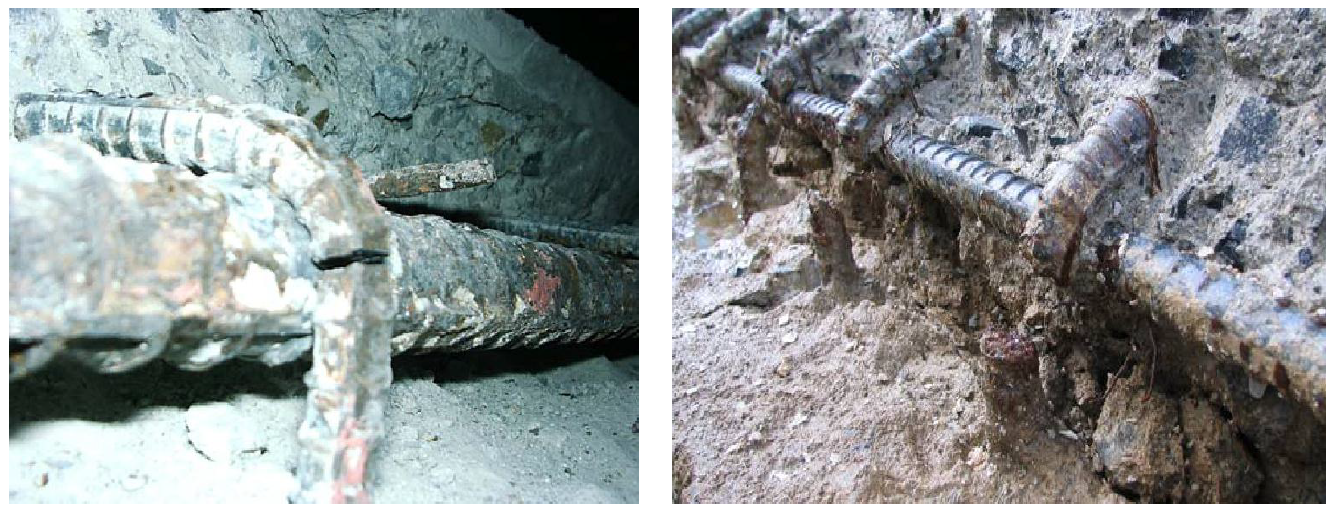
\includegraphics[width=.9\linewidth]{Files/Background/Miyagawa.png}
        \caption{Fractured stirrups in ASR-affected bridge piers in Japan [Miyagawa, et al. 2006, Torii, et al. 2008].}
        \label{fig:Miyagawa}
    \end{figure}

% DEF Examples

% ANUPUMN

Investigation done by A. Awasthi\cite{Awasthi} reveals large ettringite deposition in the damaged sleepers of Indian Railways.

    \begin{figure}[ht!]
        \centering
        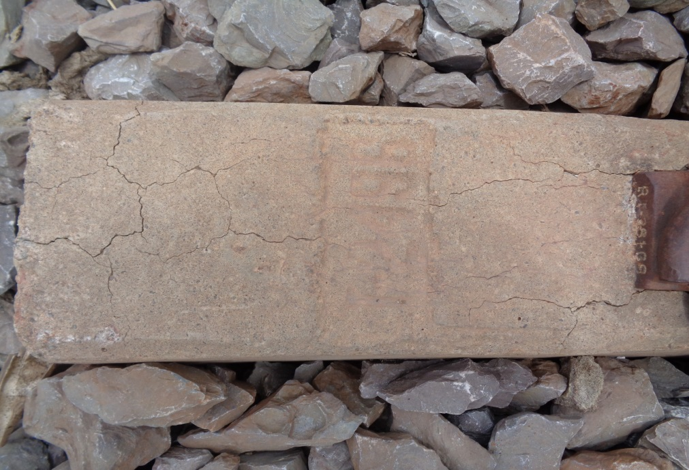
\includegraphics[width=.6\linewidth]{Files/Background/Anupam_1.png}
        \caption{Premature cracking of sleepers in Indian Railways[A. Awasthi, 2016].}
        \label{fig:Awasthi_1}
    \end{figure}

The problem of pre-mature cracking is investigated by collecting extensive samples from Indian Railways, studying the manufacturing processes, measured temperature inside concrete sleepers in the set up of a concrete sleeper plant, and analyzing samples using SEM (Scanning Electron Microscope), EDS (Energy-dispersive X-ray Spectroscopy) and XRF (X-ray Fluorescence).

In this research, EDS analysis confirmed the composition of DEF. Also, field measurement of temperature reveals that sleepers experiences high early age temperature (> 80$^\circ$C ), which is very critical for DEF problem to occur in future.

    \begin{figure}[ht!]
        \centering
        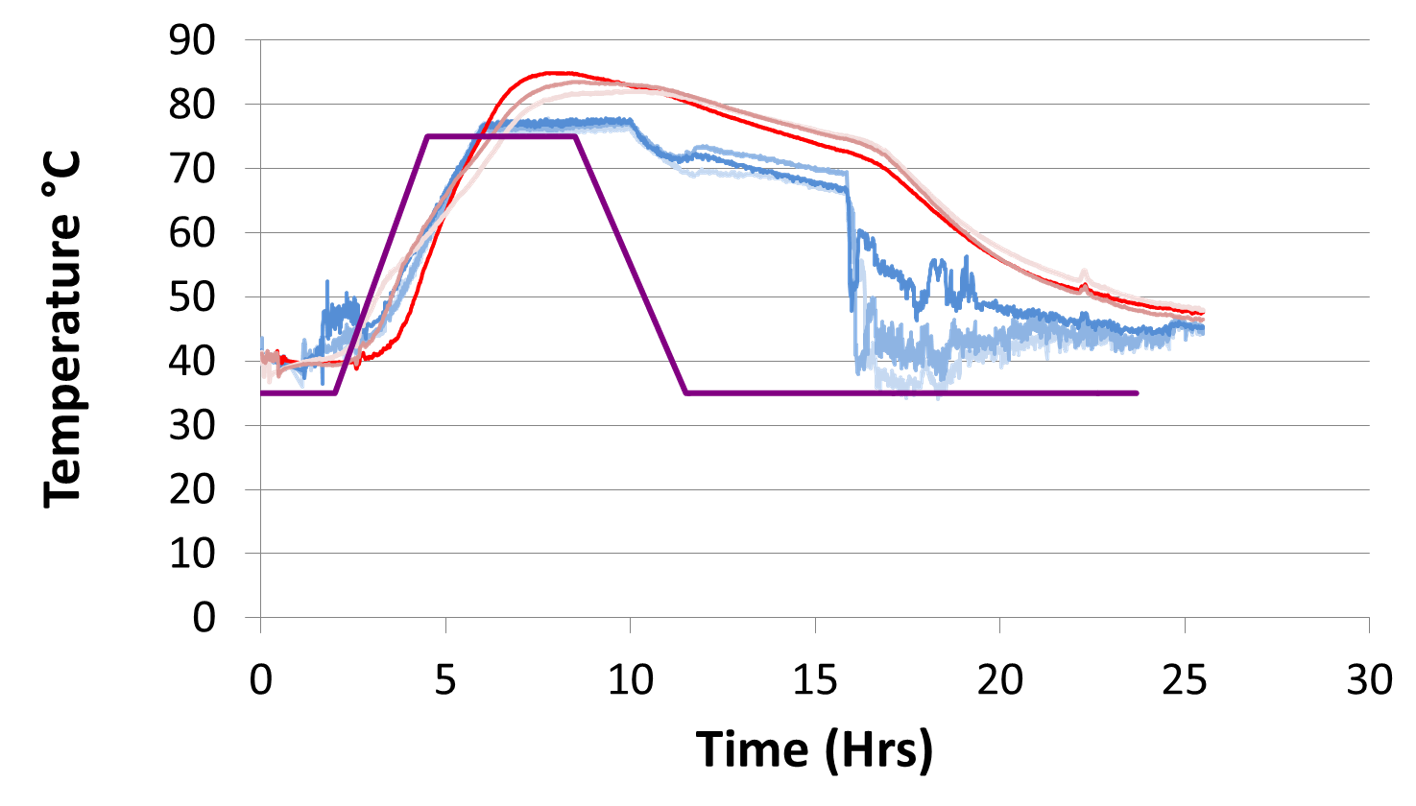
\includegraphics[width=.8\linewidth]{Files/Background/Anupam_2.png}
        \caption{Results of field measurement of temperature
 of sleepers during curing process in Indian Railways[A. Awasthi, 2016].}
        \label{fig:Awasthi_2}
    \end{figure}

Besides, in many cases, DEF has been accompanied by ASR, and may have been triggered in part by ASR (Folliard et al. 2006)\cite{Folliard}.

As a result of considerable research advances, ASR and DEF are now avoidable in new construction, but evaluating and managing the existing stock of structures damaged by these mechanisms remains a challenge.

Therefore, investigating how expansion from ASR and DEF affects on mechanical properties of concrete was the principal aim of this study.

In order to reach various expansion result, combinations such as different aggregate volume and different reactive aggregate were tried out by using concrete cube, 100x100x100 mm in size. By expanding the concrete model up to 1.3 percent, the relationship between mechanical properties losses and expansion can also be analyzed.

%*******10********20********30********40********50********60********70********80
\section{Literature Review}

\begin{itemize}

    \item
    \textbf{Evaluation of Concrete Structures Affected by Alkali-Silica Reaction and Delayed Ettringite Formation, E.R.Giannini, 2012}

    Four primary types of exposure site specimens were fabricated for this study, including Block, Unreinforced Slab-on grade, Reinforced Column, and Reinforced Bridge Deck, done by  E.R.Giannini in 2012\cite{GIANNINI}.

    Aggregate in different level of reactivity are used for the exposure site specimens. Portland cements with high alkali contents were accelerated with 50\% w/w NaOH solution to ensure that all specimens would undergo significant expansions within the time constraints of the project.

    \begin{figure}[ht!]
        \centering
        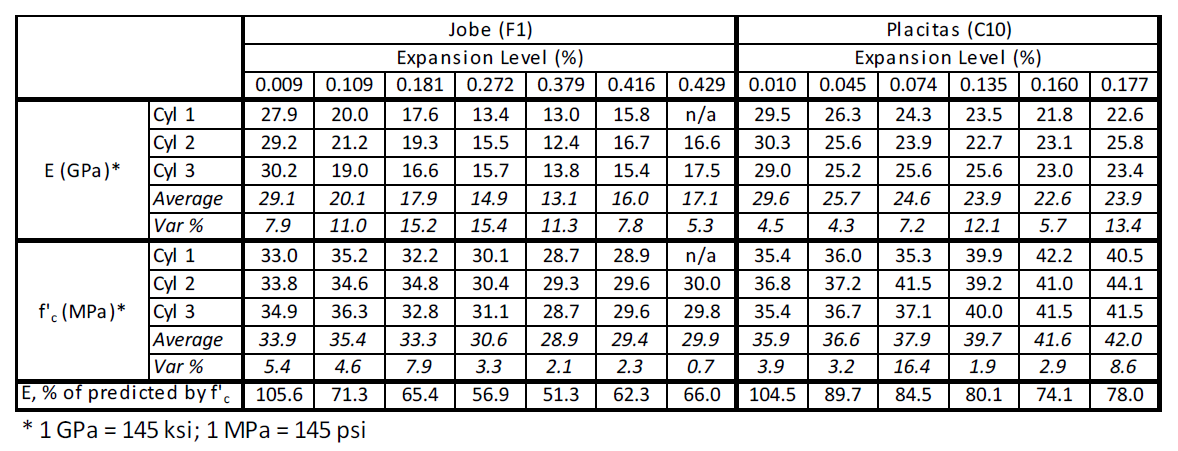
\includegraphics[width=.9\linewidth]{Files/Background/GIANNINI_ASR.png}
        \caption{Elastic modulus and compressive strength results for ASR cylinders. [E.R.Giannini, 2012].}
        \label{fig:GIANNINI_DEF}
    \end{figure}

    Additional procedures were involved to encourage the development of DEF. The cement and aggregates were heated in sealed buckets to 60$^\circ$C before mixing, while the mixing water was heated to 38$^\circ$C. The fresh concrete was quickly transported to a 60$^\circ$C chamber, placed and consolidated in foam-insulated wood forms. The forms were then covered in heavy blankets to minimize heat loss. After twelve hours, the heater for the chamber was turned off. The chamber was opened and the specimen allowed to slowly cool to ambient temperatures. Thermocouples recorded the temperature in the top, middle and base of the specimen. Peak curing temperature were well above the threshold necessary for the development of DEF.

    \begin{figure}[ht!]
        \centering
        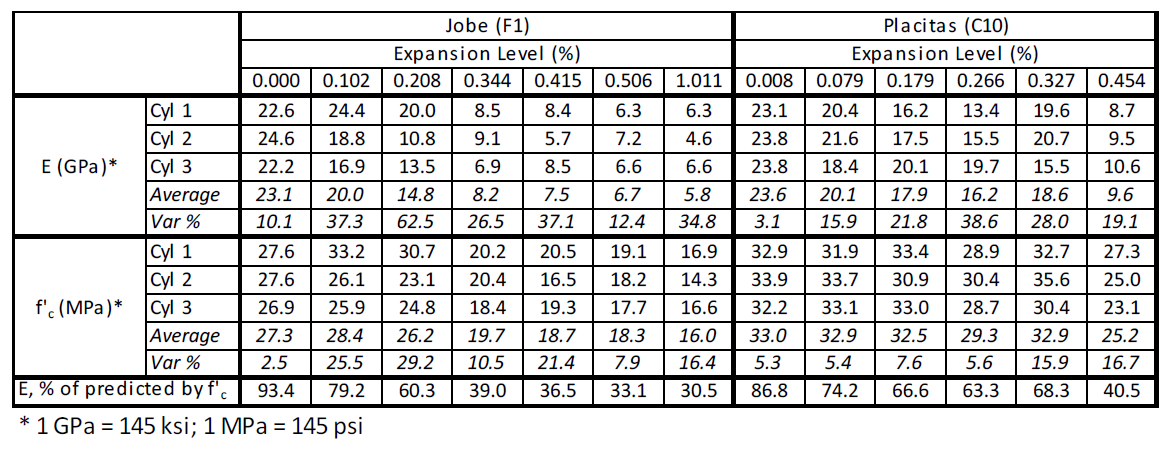
\includegraphics[width=.9\linewidth]{Files/Background/GIANNINI_DEF.png}
        \caption{Elastic modulus and compressive strength results for DEF cylinders. [E.R.Giannini, 2012].}
        \label{fig:GIANNINI_DEF}
    \end{figure}


    \item
    \textbf{The Effect Of Alkali Reactivity On the Mechanical Properties Of Concrete, T. Ahmed et al, 2013}

    In this study, T. Ahmed\cite{Ahmed} et al. used Thames Valley sand (in Mix A), fused silica (in Mix B) and slowly reactive aggregate (in Mix C) to investigate the effect of ASR expansion on compressive strength of concrete. Specimens in 100x100x100 size were cast and cured with respect to BS 1881 Part 122 [BS, 1881]. After casting and moulding, the cube specimens were cured for 28 days in water at $20^\circ$C and then the temperature was increased to $38^\circ$C to accelerate alkali-silica reaction. In this temperature, the specimens were stored at water tank until 12 months passed [Ahmed et al., 2003]. After 28-days curing at $20^\circ$C and storage at $38^\circ$C for 12 months, surface cracks are observed (Figure \ref{fig:T.Ahmed_crack}), and the expansion ratios along with compressive strength are given in Table \ref{table:Ahmed et al.}.

    \begin{figure}[ht!]
        \centering
        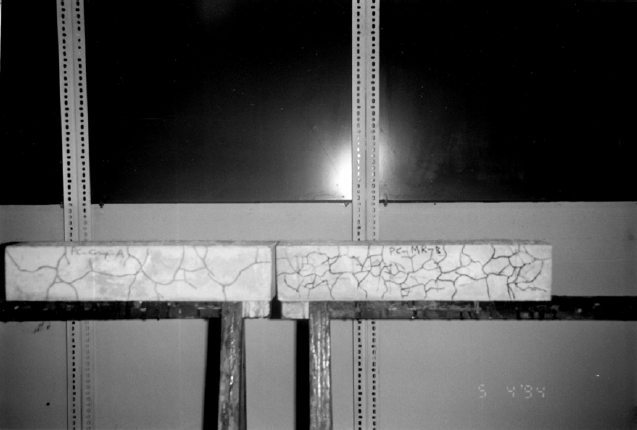
\includegraphics[width=.6\linewidth]{Files/Background/Ahmed_crack.png}
        \caption{Crack pattern of horizontally cast concrete prismcontaining Thames Valley sand (mix A) and 15\% fused silica (mix B) [Ahmed et al., 2003].}
        \label{fig:T.Ahmed_crack}
    \end{figure}

    \begin{table}[ht!]
        \centering
            \begin{tabular}{ |p{6cm}|p{1.5cm}|p{1.5cm}|p{1.5cm}| }
             \hline
             Mix &  A & B & C  \\ [0.5ex]
             \hline
             Expansion ratio (mm/mm) for 28-days curing at $20^\circ$C & -0.4 & 0.96 & 0.05 \\
             \hline
             Compressive Strength ($N/mm^2$) for 28-days curing at $20^\circ$C & 50.3 & 41.0 & 46.8 \\
             \hline
             Expansion ratio (mm/mm) for 12 months curing at $38^\circ$C & 4.3 & 16.86 & 1.27 \\
             \hline
             Compressive Strength ($N/mm^2$) for 12 months curing at $38^\circ$C & 57.0 & 26.5 & 65.3 \\ [0.5ex]
             \hline
            \end{tabular}
        \caption{Effect of ASR expansion on compressive strength of concrete [Ahmed et al., 2003].}
        \label{table:Ahmed et al.}
    \end{table}


    \item
    \textbf{Investigation of Premature Cracking of Sleepers in Indian Railways \& Evaluation of It's Residual Capacity, A. AWASTHI et al, 2016}

      In this study, A. Awasthi\cite{Awasthi} investigated the damaged premature cracking of sleepers, using the Scanning Electron Microscope (SEM) and Energy-Dispersive X-Ray Spectroscopy(EDS), confirmed the existing of DEF phenomenal in damaged concrete sleepers.

      \begin{figure}[ht!]
          \centering
          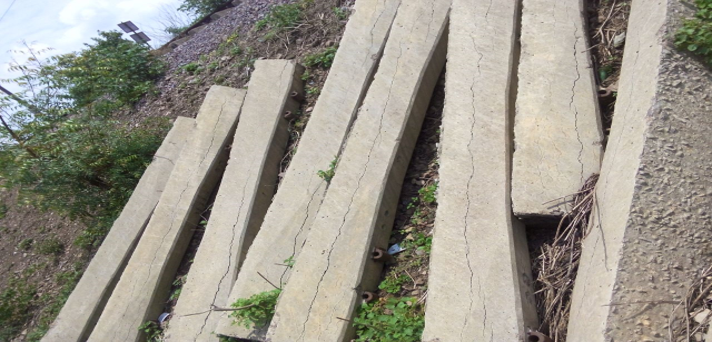
\includegraphics[width=.8\linewidth]{Files/Background/Anupam_3.png}
          \caption{Premature cracking of sleepers in Indian Railways[A. Awasthi, 2016].}
          \label{fig:Awasthi_3}
      \end{figure}

      The pre-heating process done on these concrete sleepers in order to achieve a high early strength (in case of Indian concrete sleepers the steam curing temperature is 75 $^\circ$C) and subsequent exposure to moisture during service lead the formation of delayed ettringite. Temperature measurement was performed in concrete sleeper plant in India both inside and outside of concrete reveals that temperature inside the concrete sleeper is much higher than the outer part, the high temperature over 80$^\circ$C is a very critical factor for the occurrence of damage due to DEF.

      \begin{figure}[ht!]
          \centering
          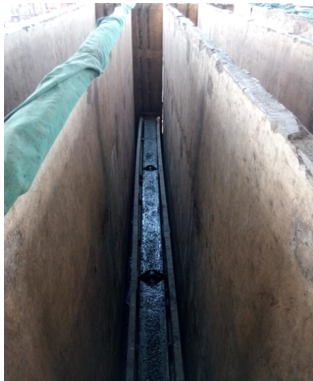
\includegraphics[width=.6\linewidth]{Files/Background/Anupam_4.png}
          \caption{Temperature measurement for pre-heating process of Indian Concrete Sleeper [A. Awasthi, 2016].}
          \label{fig:Awasthi_4}
      \end{figure}

    \clearpage
    \item
    \textbf{Mesoscopic analysis of different expansion causes in concrete by 3D Rigid Body Spring Model, L. EDDY, A. AWASTHI, K, MATSUMOTO, K. NAGAI, and S.ASAMOTO, 2017}

    This study done by L. EDDY et al.\cite{Eddy} developed the 3 dimensional numerical discrete analysis model using RBSM for mesoscopic analysis of different expansion, including both ASR expansion and DEF expansion.


    \begin{figure}[ht!]
    \centering
    \begin{subfigure}{.5\textwidth}
      \centering
      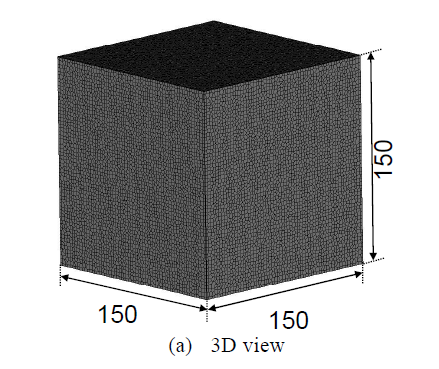
\includegraphics[width=.9\linewidth]{Files/Background/EDDY_model_1.png}
    \end{subfigure}%
    \begin{subfigure}{.5\textwidth}
      \centering
      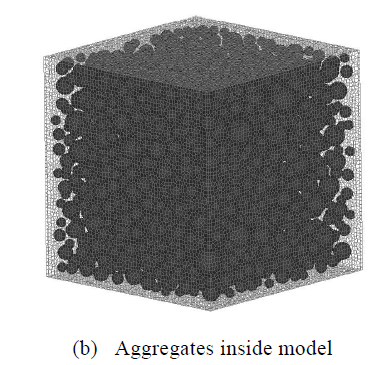
\includegraphics[width=.75\linewidth]{Files/Background/EDDY_model_2.png}
    \end{subfigure}
    \caption{3D Concrete Model (units: mm) [L.EDDY et al.]}
    \label{fig:EDDY_model}
    \end{figure}

    Fig \ref{fig:EDDY_model} shows the analyzed numerical model. The size of the model is 150x150x150 mm. Aggregate volume is 26\% in this research.

    \begin{figure}[ht!]
        \centering
        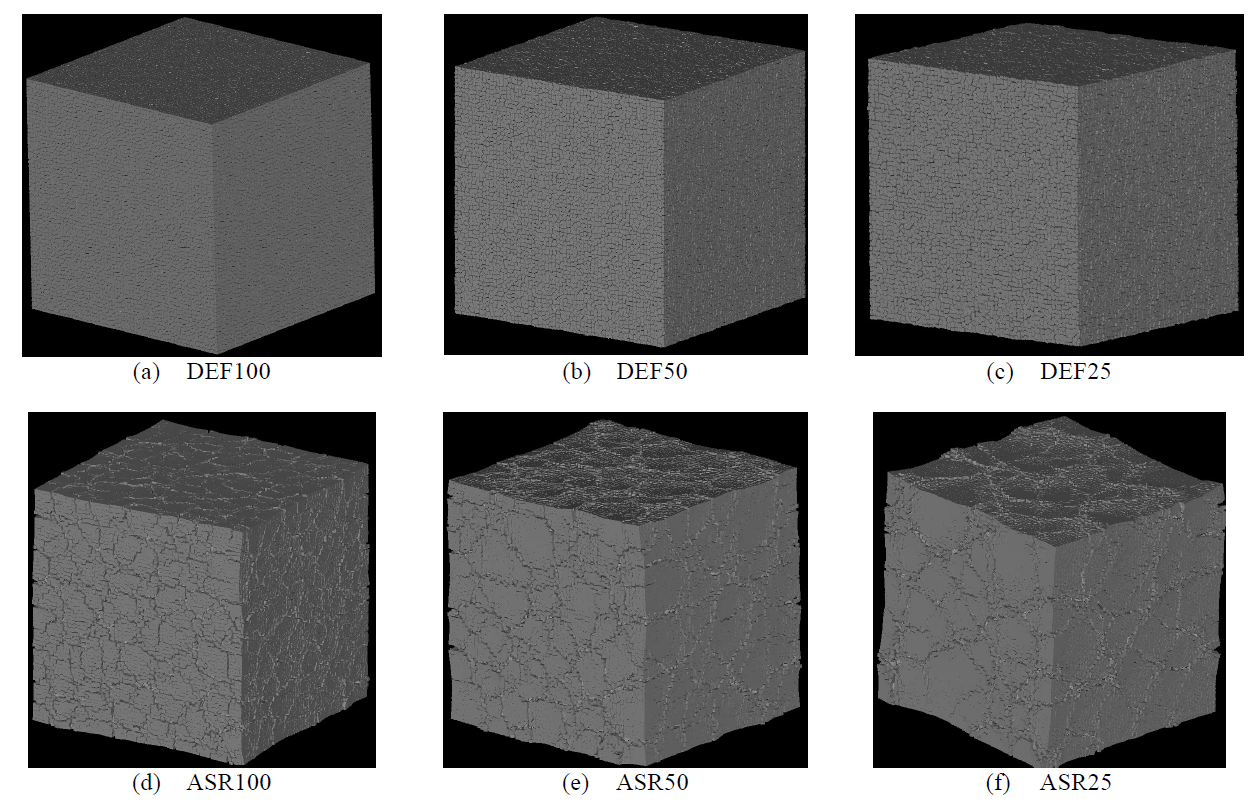
\includegraphics[width=.9\linewidth]{Files/Background/EDDY.png}
        \caption{Surface Cracks (Deformation x 10) [L.EDDY et al.]}
        \label{fig:EDDY}
    \end{figure}

    In the ASR-type cases, the expansion strain is applied at the mortar-aggregate interfaces to reflect the expansion due to the alkali silicate gel product formed in the aggregates.

    Three numerical models, named by ASR100, ASR50, and ASR25 are considered in ASR simulations. ASR100 means that all the mortar-aggregate interfaces expand. ASR50 means that 50\% of all springs between mortar-aggregate interfaces (randomly selected) expand. While ASR25 means that 25\% of all springs between mortar-aggregate interfaces (randomly selected) expand.

    Stress in the aggregates and mortar decreases because localized cracks in the mortar open. With less percentage of locations of the mortar-aggregate interface expansion, cracks become more localized. These localized cracks int he mortar and the expansion at the mortar-aggregate interfaces are connected to form the map cracks occur in the concrete.

    In the cases for DEF-type, the expansion strain is applied in the mortar to represent the paste expansion. However, based on the simulation results, DEF-type cases do not match well with the typical map cracking pattern observed in the real concrete.

    Meanwhile, three numerical models, named by DEF100, DEF50, DEF25 are considered in this DEF simulations. DEF100 means that all springs between mortar elements expand. DEF50 means that 50\% of all springs between mortar elements (randomly selected) expand. While DEF25 means that 25\% of all springs between mortar elements (randomly selected) expand.

    E. Liyanto and team proposed that simple model as uniform expansion of paste takes place in DEF could not reproduce the typical cracking pattern of DEF. In order to simulate the DEF appropriately, the simple model in this study needs to be improved because there might be more complex phenomenon occurred.

\end{itemize}

%*******10********20********30********40********50********60********70********80

\section{Deformation Mechanism for ASR and DEF}

ASR and DEF, though produce similar visual indications (charcteristic map surface cracking), the mechanism of each is different. A short discussion of the two mechanisms is provided below.

\subsection{Alkali-Silica Reaction (ASR)}

Firstly identified by Stanton\cite{Stanton} over 70 years ago, ASR is a important reason of concrete deterioration. Since that time, ASR has been identified as a cause of deterioration of numerous concrete structures.

%Stanton, T. E. "Expansion of Concrete through Reaction between Cement and Aggregate." Publications of the American Society of Civil Engineers 66 (1940): 1781-1811.

Alkali silica reaction (ASR) is a deleterious chemical reaction, between some siliceous minerals in the aggregate and the alkalinity of the concrete.

As the result, a hydrophilic gel named ASR gel is formated and swells in the presence of moisture, causing the expansion of concrete. Figure \ref{ASR_mechanism} by Kreitman, K\cite{Kreitman} illustrates the mechanism of ASR.

%Kreitman, K. "Nondestructive Evaluation of Reinforced Concrete Structures Affected by Alkali-Silica Reaction and Delayed Ettringite Formation." MS Thesis, The University of Texas at Austin, Austin, Texas, 2011.

\begin{figure}[ht]
\centering
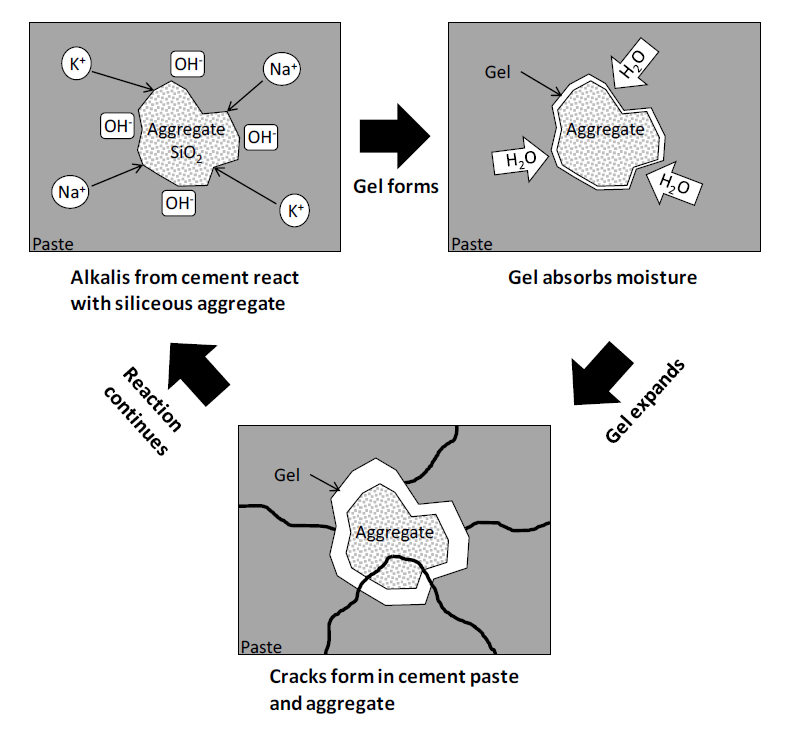
\includegraphics[width=.8\linewidth]{Reference/Kreitman.png}
  \caption{Mechanism of alkali-silica reaction [Kreitman 2011]}
  \label{ASR_mechanism}
\end{figure}

According to G.K. Glass\cite{Glass} in book Comprehensive Structural Integrity, 2003, factors which control the reaction rate and degree of expansion include the alkali content, the quantity of reactive aggregate and its particle size, the moisture content of the concrete and moisture content variations, temperature and the permeability of the concrete.

%G.K. Glass, in Comprehensive Structural Integrity, 2003

Although countermesures has yielded considerable success in minimize the risk of expansive ASR in new construction, the capability of ASR damaged concrete remains a major topic of ongoing research.

%%%%%%%%%%%%%%%%%%%%%%%%%%%%%%%%%%%%%%%%%%%%%%%%%%%%
\subsection{Delayed Ettringite Formation (DEF)}

Delayed Ettringite Formation (DEF) is a form of internal sulfate attack in concrete, driven by high curing temperatures and unfavorable cement chemistry (Kelham 1996\cite{Kelham}). Many laboratory studies have confirmed that 70$^\circ$C is the critical curing temperature for expansion due to DEF(H.F.W. Taylor et al., 2000\cite{Taylor}).

%Kelham, S. "The Effect of Cement Composition and Fineness on Expansion Associated with Delayed Ettringite Formation." Cement & Concrete Composites 18 (1996): 171-179.

%H.F.W Taylor, C. Famy, K.L. Scrivener. "Review: Delayed Ettringite Formation", Cement and Concrete Research 31(2001) 683-693

The hydration of cement and formation of C-S-H is greatly accelerated as curing temperature increases (Folliard, et al. 2006\cite{Folliard}). The rapidly growing “outer” C-S-H is different than that which forms at lower temperatures and traps dissolved sulfates before they can react to form ettringite, another normal product of cement hydration. With sustained temperatures above 70$^\circ$C, ettringite becomes thermodynamically unstable and either does not form or returns to solution.

%Folliard, K. J., et al. Preventing ASR/DEF In New Concrete: Final Report. Austin: Center for Transportation Research, 2006.

 Based on thermodynamics and X-ray diffraction observations, other hydration products, stable at high temperatures, such as calcium monosulfoaluminate (monosulfate) and hydrogarnet form instead from the decomposing ettringite and remaining aluminates, ferrites and sulfates in solution (Ramlochan 2003\cite{Ramlochan}).

 %Ramlochan, T. "The Effects of Pozzolans and Slag on the Expansion of Mortars and Concrete Cured at Elevated Temperature." PhD Thesis, Toronto: University of Toronto, 2003.

Once temperatures return to normal level, thermodynamics assist the formation of ettringite. Sulfates may be released from the C-S-H, then react with water and monosulfate, form ettringite, and lead to deleterious expansion and cracking of the concrete (Folliard et al, 2006\cite{Folliard}). A illustration of the mechanism of DEF is shown in Figure \ref{DEF_mechanism}.

 \begin{figure}[ht]
 \centering
 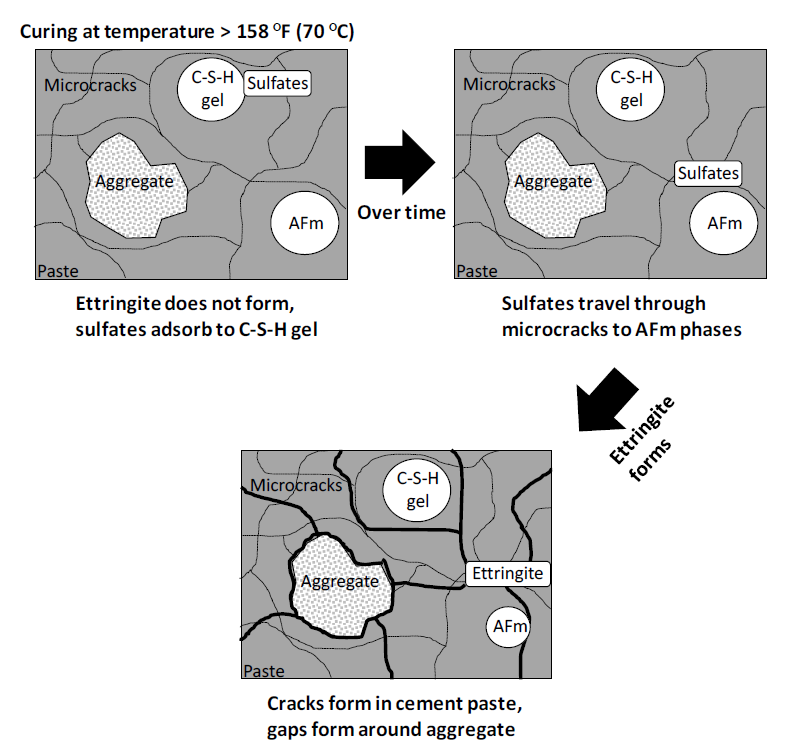
\includegraphics[width=.8\linewidth]{Reference/Kreitman2.png}
   \caption{Mechanism of delayed ettringite formation [Kreitman 2011]}
   \label{DEF_mechanism}
 \end{figure}


%*******10********20********30********40********50********60********70********80
\section{Research Objective}

The final goal of this research is to develop the simulation system which has ability for revealing the residual capacity of ASR and DEF expansion deteriorated structure.

Considering our research group’s simulation systems, 3D RBSM was conducted for the quantities evaluation of concrete behavior by directly modeling the shape of aggregates.

Considering the previous study about the expansion of concrete structure in literature review, in order to achieve the final goal, the following objectives are set as the research’s goal:

\begin{itemize}

    \item Develop the simulation of concrete damage from the ASR expansion. Once the ASR expanse occurred, the initial strain will be given at the interfaces between reactive aggregate and mortar. As a result, increasing of tensile stress of concrete around the reactive aggregate will lead to the cracking.

    \item Develop the simulation of concrete damage from the DEF expansion. Once the DEF expanse occurred, the initial strain will be given at the interfaces between mortar elements. As a result, increasing of tensile stress of inside concrete paste will lead to the cracking.

    \item Develop the uni-axial compression test for represent the residual mechanical properties of expanded concrete models. Concrete's behavior under loading and its proprieties such as compressive strength and elastic modulus in macro scale will be obtained.

\end{itemize}



%*******10********20********30********40********50********60********70********80
\section{Organization of Contents}

The development of simulation and mechanical properties test in ASR and DEF expanded concrete will be explained in this thesis following structure as shown below:

\begin{itemize}

    \item Chapter 1 : Introduction.

    In this chapter, detailed about research background, statement of problem and objective are explained. Some literature reviews that related to the developing.

    \item Chapter 2 : Simulation Model.

    In this chapter, the method in development of each numerical simulation model, related literature review of previous studies, will be described. The development of constitutive model for the expansion will be explained. The method for given expansive strain for simulating the same concrete damage will be explain step by step. The theoretical formulation related in numerical analysis of expanding behaviour are also described in this section.

    \item Chapter 3: Simulation of Cracking Pattern Of ASR and DEF Expanded Concrete.

    In this chapter, details about the surface and cross section cracking pattern results caused by ASR and DEF expansion are summarized, comparing between different cases and also with the experimental results.

    \item Chapter 4: Simulation of Residual Mechanical Capabilities Of ASR and DEF Expanded Concrete.

    In this chapter, details about the residual mechanical properties, including residual compressive strength and residual elastic modulus, are summarized. The relationships between residual capacity and expansion behavior due to different expansion causes are also discussed.

    \item Chapter 5: Conclusions

    In this final chapter, several remarks about the capability of ASR and DEF expansion simulation are emphasized. Also, some commentaries for further project and improvement are proposed.


\end{itemize}
 

 %*******10********20********30********40********50********60********70********80

% For all chapters, use the new defined chap{} instead of chapter{}
% This will make the text at the top-left of the page be the same as the chapter

\chap{Method of Simulation Models}

\section{Rigid Body Spring Model (RBSM)}

The simulations are carried out by the three dimensional RBSM, proposed by Kawai \textit{et al}.(1978). By using 3D RBSM, a concrete model is meshed into rigid bodies, with each consists six degree of freedoms, shown in Figure \ref{fig:RBSM}.

\begin{figure}[ht!]
\centering
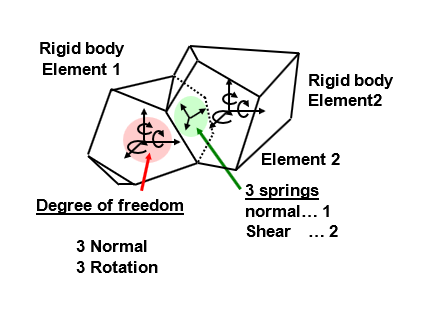
\includegraphics[width=.4\linewidth]{Files/Background/RBSM_1.png}
  \caption{Rigid Body Spring Model}
  \label{fig:RBSM}
\end{figure}

These six freedoms are three transitional freedoms and three rotational freedoms at the center point within the element.

The computational point $(x_c, y_c, z_c)$ is defined as,

\begin{equation}
  \begin{aligned}
  &x_c=\frac{x_1 + x_2 + \cdots + x_i + \cdots + x_m}{m} \\
  &y_c=\frac{y_1 + y_2 + \cdots + y_i + \cdots + y_m}{m} \\
  &z_c=\frac{z_1 + z_2 + \cdots + z_i + \cdots + z_m}{m}
  \end{aligned}
\end{equation}

where m is the number of node composing an element and $x_i$, $y_i$ and $z_i$ are the coordinates of the nodes in an element.

Three individual springs, which are one normal spring and two shear spring, are set at a point on the face between two elements. This point $(x_{cf}, y_{cf}, z_{cf})$ is defined as,

\begin{equation}
  \begin{aligned}
  &x_{cf}=\frac{x_1 + x_2 + \cdots + x_j + \cdots + x_n}{n} \\
  &y_{cf}=\frac{y_1 + y_2 + \cdots + y_j + \cdots + y_n}{n} \\
  &z_{cf}=\frac{z_1 + z_2 + \cdots + z_j + \cdots + z_n}{n}
  \end{aligned}
\end{equation}

Where m is the number of nodes composing the face and $x_j$, $y_j$ and $z_j$ are those coordinates.

Since cracks initiate and propagate along the boundary face, the mesh arrangement may affect fracture direction. Random geometry is introduced to avoid the formation of cracks in a certain direction by using a Voronoi diagram
\textbf{figure}.

In the nonlinear analysis, a stiffness matrix is constructed based on the principle of virtual work (Kawai and Takeuchi 1990), and the Modified Newton-Raphson method is employed for the convergence algorithm.

When an element has small displacement $[u_1, v_1, w_1, \theta_{u1}, \theta_{v1}, \theta_{w1}]$, the springs at a face in an element will be displaced:

\begin{equation}
  \begin{aligned}
  &u = u_1 - \theta_{w1} (y_{cf} - y_{ce1}) + \theta_{v1} (z_{cf} - z_{ce1}) \\
  &v = v_1 - \theta_{u1} (z_{cf} - z_{ce1}) + \theta_{w1} (x_{cf} - x_{ce1}) \\
  &w = w_1 - \theta_{v1} (x_{cf} - x_{ce1}) + \theta_{u1} (y_{cf} - y_{ce1})
  \end{aligned}
\end{equation}

Elongations of normal and shear spring are calculated and expressed as:

\begin{equation}
  d = Bu_e
\end{equation}

where $d^T = [\delta_{s1}, \delta_{s2}, \delta_n]$ and $u_e^T = [u_1, v_1, w_1,\theta_{u1}, \theta_{v1}, \theta_{w1}, u_2, v_2, w_2,\theta_{u2}, \theta_{v2}, \theta_{w2}]$

The transformation matrix B is written as:

\begin{equation}
  B =
  \begin{vmatrix}
    K_{11} &K_{12} &K_{13} &K_{14} &{\cdots} &K_{19} &K_{110} &K_{111} &K_{112}\\
    K_{21} &K_{22} &K_{23} &K_{24} &{\cdots} &K_{29} &K_{210} &K_{211} &K_{212}\\
    K_{31} &K_{32} &K_{33} &K_{34} &{\cdots} &K_{39} &K_{310} &K_{311} &K_{312}
  \end{vmatrix}
\end{equation}

where \\
$K_{11} = -e_{s1x}$    $K_{21} = -e_{s2x}$    $K_{31} = -e_{nx}$ \\
$K_{12} = -e_{s1y}$    $K_{22} = -e_{s1y}$    $K_{32} = -e_{ny}$ \\
$K_{13} = -e_{s1z}$    $K_{23} = -e_{s2z}$    $K_{33} = -e_{nz}$ \\
\\
$K_{14} = e_{s1y}(z_{cf}-z{ce1})-e_{s1z}(y_{cf}-y_{ce1})$\\
$K_{24} = e_{s2y}(z_{cf}-z{ce1})-e_{s2z}(y_{cf}-y_{ce1})$\\
$K_{34} = e_{ny}(z_{cf}-z{ce1})-e_{nz}(y_{cf}-y_{ce1})$\\
\\
$K_{15} = e_{s1z}(x_{cf}-x{ce1})-e_{s1x}(z_{cf}-z_{ce1})$\\
$K_{25} = e_{s2z}(x_{cf}-x{ce1})-e_{s2x}(z_{cf}-z_{ce1})$\\
$K_{35} = e_{nz}(x_{cf}-x{ce1})-e_{nx}(z_{cf}-z_{ce1})$\\
\\
$K_{15} = e_{s1z}(x_{cf}-x{ce1})-e_{s1x}(z_{cf}-z_{ce1})$\\
$K_{25} = e_{s2z}(x_{cf}-x{ce1})-e_{s2x}(z_{cf}-z_{ce1})$\\
$K_{35} = e_{nz}(x_{cf}-x{ce1})-e_{nx}(z_{cf}-z_{ce1})$\\
\\
$K_{16} = e_{s1x}(y_{cf}-y{ce1})-e_{s1y}(x_{cf}-x_{ce1})$\\
$K_{26} = e_{s2x}(y_{cf}-y{ce1})-e_{s2y}(x_{cf}-x_{ce1})$\\
$K_{36} = e_{nx}(y_{cf}-y{ce1})-e_{ny}(x_{cf}-x_{ce1})$\\
\\
$K_{17} = e_{s1x}$    $K_{27} = e_{s2x}$    $K_{37} = e_{nx}$ \\
$K_{18} = e_{s1y}$    $K_{28} = e_{s1y}$    $K_{38} = e_{ny}$ \\
$K_{19} = e_{s1z}$    $K_{29} = e_{s2z}$    $K_{39} = e_{nz}$ \\
\\
$K_{110} = e_{s1z}(y_{cf}-y{ce2})-e_{s1y}(z_{cf}-z_{ce2})$\\
$K_{210} = e_{s2z}(y_{cf}-y{ce2})-e_{s2y}(z_{cf}-z_{ce2})$\\
$K_{310} = e_{nz}(y_{cf}-y{ce2})-e_{ny}(z_{cf}-z_{ce2})$\\
\\
$K_{111} = e_{s1x}(z_{cf}-z{ce2})-e_{s1z}(x_{cf}-x_{ce2})$\\
$K_{211} = e_{s2x}(z_{cf}-z{ce2})-e_{s2z}(x_{cf}-x_{ce2})$\\
$K_{311} = e_{nx}(z_{cf}-z{ce2})-e_{nz}(x_{cf}-x_{ce2})$\\
\\
$K_{112} = e_{s1y}(x_{cf}-x{ce2})-e_{s1x}(y_{cf}-y_{ce2})$\\
$K_{212} = e_{s2y}(x_{cf}-x{ce2})-e_{s2x}(y_{cf}-y_{ce2})$\\
$K_{312} = e_{ny}(x_{cf}-x{ce2})-e_{nx}(y_{cf}-y_{ce2})$\\

where $e_{ij}$ is direction cosine in i axis on j axis.

By applying the principal of virtual work, the local equilibrium relation expressed in global coordinate is:

\begin{equation}
  k_e \delta u_e = \delta f_e
\end{equation}

where the stiffness associated with interconnected face $k_e$ is given as:

\begin{equation}
  k_e = B^T DB
\end{equation}

where
\begin{equation}
  D = \begin{vmatrix}
        k_{s1} &0 &0 \\
        0 &k_{s2} &0 \\
        0 &0 &k_3
      \end{vmatrix}
\end{equation}

in which $k_n$, $k_{s1}$, and $k_{s2}$ are the normal and shear spring stiffness. $k_n$, $k_{s1}$, and $k_{s2}$ can be calculated as:
\begin{equation}
  \begin{aligned}
    &k_n = k_{sp} \frac{A}{h_1 + h_2} \\
    &k_{s1} = k_{ssp} \frac{A}{h_1 + h_2} \\
    &k_{s2} = k_{ssp} \frac{A}{h_1 + h_2}
  \end{aligned}
\end{equation}

where

\begin{equation}
  \begin{aligned}
    &k_{nsp} = \frac{(1-\theta_{elem})E_{elem}}{(1+\theta_{elem})(1-2\theta_{elem})} \\
    &k_{ssp} = \frac{E_{elem}}{1+\theta_{elem}}
  \end{aligned}
\end{equation}

where $h_1$ and $h_2$ are length of perpendicular lines from the element computational point to the face where springs are set.

$E_{elem}$ and $v_{elem}$ are the modulus of elasticity and poison's ratio, respectively:

\begin{equation}
  \begin{aligned}
    &E_{elem} = \frac{E_{elem1} h_1 + {E_{elem2} h_2}}{h_1+h_2} \\
    &\theta_{elem} = \frac{\theta_{elem1} h_1 + {\theta_{elem2} h_2}}{h_1+h_2}
  \end{aligned}
\end{equation}

In the convergence process, displacements that cancel the unbalanced force of elements are added to the elements.

The displacements are calculated using the stiffness matrix. Convergence of the model is judged when the ratio of
$\sum_{} $(Unbalanced force of element in the model)$^2$ to \\
$\sum_{} $(Applied force to element)$^2$ becomes less than $10^5$.
%*******10********20********30********40********50********60********70********80

%*******10********20********30********40********50********60********70********80
\section{Rigid Body Spring Model (RBSM)}

A constitutive model for the concrete part at the mesoscale is used in this research since constitutive model in the macro scale cannot be applied to the mesoscale analysis.

In the analysis, the values of the material properties at the meso level given to the elements are actually different from the material properties where the object is analyzed at the macroscopic scale.

The material properties for the elements were determined to give the correct macroscopic properties.  In the discrete analysis done by Nagai et al. in 2005, the shape and fineness of elements do affect the analysis results.

As we concern that the crack direction may affect the crack pattern, size of each concrete elements should be under consideration. Here for small example using 10x10x10mm model, the average diameter of elements is selected to be 0.05mm, while for larger size model in the dimension of 100x100x100mm, the size of each element is approximately 2x2x2mm to 3x3x3mm, almost the size of smallest coarse aggregate introduced. This assumption was made to represent the fracture behavior in concrete in a relatively high fineness and the behavior of both mortar and aggregate can be well presented.

In the elastic analysis, the relationship between macroscopic and mesoscopic Poisson's ratio, the effect of the mesoscopic Poisson's ratio on the macroscopic elastic modulus, are all confirmed by Nagai et al. in 2005, using the same concepts.

\begin{equation}
  \begin{aligned}
  &\theta_{elem} = -24.8\theta^4+31.9\theta^3-16.4\theta^2 +4.28\theta\\
  &E_{elem} = (-33.7\theta_{elem}^4 + 17.0\theta_{elem}^3 - 4.13\theta_{elem}^2 + 0.327\theta_{elem} + 1)E
  \end{aligned}
\end{equation}

where E and $\theta$ are the macroscopic elastic modulus and Poisson's ratio of the analysis object, respectively.

The material characteristics of each component are presented by means of modeling springs. In normal spring, compressive and tensile stress ($\sigma$) are developed. Shear stress($\tau$) are developed by shear springs.

The elastic modulus of normal sprint($k_{nsp}$ and $k_{ssp}$) was presented in the previous chapter. For calculation of shear stress on 3D analysis, a resultant value of strains generated in two shear springs is adopted as shear strain in the constitutive model presented in this chapter. The strains and stress are calculated as follows:

\begin{equation}
  \begin{aligned}
  &\varepsilon = \frac{\delta_n}{h_1 + h_2}\\
  &\gamma = \frac{\delta_s}{h_1 + h_2}\\
  &\sigma = k_{nsp}\varepsilon\\
  &\tau = k_{ssp}\gamma
  \end{aligned}
\end{equation}

where $\varepsilon$ and $\gamma$ are the strain of normal and shear springs, respectively. $\delta_n$ and $\delta_s$ are the normal and shear relative displacement of elements of those springs, respectively.

In this study, the constitutive model of the concrete element has been developed based on simulations in material scale level. The constitutive models for the normal and shear springs of the concrete elements are shown in Figure %TODO:\ref{}.

%TODO: EDDY P32

The constitutive models of normal spring and a shear spring of concrete element using in this research are shown in Figure %TODO: \ref{}.

Basically, the concept of the concrete model is the same as the original simulation development by Nagai et al., 2005, where the compressive failure is not allowed at the mesoscale. In the tension zone, crack between two rigid bodies occurs only when the tensile stress of the normal spring exceeds the tensile strength of the concrete($f_t$). After exceeding the tensile strength($f_t$), the tensile stress of a normal spring is assumed to decrease bi-linearly, depending on the crack width, to zero at the maximum crack width($w_{max}$), which here is assumed as 0.3mm. An elasto-plastic behavior is also assumed when coming to the shear spring of concrete element with the$\tau_{max}$ is calculated based on the following equations:

\begin{equation}
  \begin{aligned}
  &\tau_{max} = \pm (1.6f_{telem}^2 (-\sigma + f_{telem})^0.4 + 0.15f_{telem}) if (\sigma \geq 3f_{telem})\\
  &\tau_{max} = \pm (1.6f_{telem}^2 (-3f_{telem} + f_{telem})^0.4 + 0.15f_{telem}) if (\sigma < 3f_{telem})
  \end{aligned}
\end{equation}

Besides, if fracture occurs in the normal spring, the calculated shear stress will be reduced according to the reduction of the normal stress. As a result, shear spring will now abole to carry the stress any longer when the crack width of the normal spring reaches $w_{max}$.


% \subsection{Mortar Model}
%
% In this study, constitutive model for concrete at meso scale is developed because constitutive model at the  macro scale cannot be applied directly to meso scale analysis.
%
% The material characteristics of each component are presented by means of modeling spring.
%
% PIC Constitutive models of concrete
%
% In normal springs, compressive and tensile stresses ($\theta$) are developed. Shear springs develop shear stress ($\tau$). The elastic modulus of normal spring ($k_n$) and shear spring ($k_s$) are presented assuming a plane strain condition, where kn and ks are the elastic modulus of normal and shear spring, and $E_{elem}$ and $v_{elem}$ are the corrected elastic modulus and Poisson’s ratio of component at the meso scale, respectively.
%
% \begin{equation}
%   \begin{aligned}
%    &\theta_{elem} = -24.8\theta^4 + 31.9\theta^3 - 16.4\theta^2 + 4.28\theta \\
%    &E_{elem} = (-33.7\theta_{elem}^4 + 17.0\theta_{elem}^3 - 4.13\theta^2 + 0.327\theta_{elem}+1)E
%   \end{aligned}
% \end{equation}
%
% For calculation of shear stress, a resultant value of strains generated in two shear springs is adopted as a shear strain in the constitutive model presented in this chapter.
%
% \begin{equation}
%   \begin{aligned}
%    &\varepsilon = \frac{\delta_n}{h_1+h_2} \\
%    &\gamma = \frac{\delta_s}{h_1+h_2} \\
%    &\sigma = k_{nsp}\varepsilon \\
%    &\tau = k_{ssp}\gamma
%   \end{aligned}
% \end{equation}
%
% \subsection{Aggregate Model}
%
% In this study, the effect of the existence of aggregate in
% concrete on the fracture process is examined. For this
% purpose, aggregate elements are assumed to behave only
% elastically without fracture in this study.
%
% The same equations as (3?), (4?), (5?) and (7?) are adopted to present the material property of aggregate.
%
% Pic Of AGGREGATE
 % \section{Rigid Body Spring Model (RBSM)}

\section{Expansion Model}

In the expansive behavior of DEF and ASR, the expanse is caused by strains generated from within the concrete when there is no external loading.

One of the similar behavior in previous research is the strength development due to autogenous shrinkage in high strength concrete, which was carried out by Osakabe et al., (2014)\cite{Osakabe}. The concept of initial strain in RBSM has been successfully utilized in the simulation of the behavior of autogenous shrinkage in high strength concrete.

The same concept of initial strain is utilized in the present of ASR and DEF expanse behavior carried out by L.EDDY et al. in 2016\cite{Eddy}. Characteristic map cracking pattern in ASR simulation was presented successfully, while the DEF simulation results do not match well with the typical map cracking pattern observed in the real concrete.

The concept of the initial strain used in this simulation is based on the case where a specimen expansion occurs without any constraint.

According to 3D RBSM developed by Nagai et al. (2005)\cite{Nagai}, the first step is the calculation of actual force, which supposed to be calculated by solving strain, stress and force matrices of all elements in sequence based on input data and boundary condition.

Iteration is then performend until this force under the acceptable limit with an external force. When the convergence condition is reached, the same sequence will be performed for the next step.

In our simulation, one additional step of introducing the initial strain is added here to simulate the behavior of expansion. Then, Stresses due to this initial strain are calculated in the next step, with considering the initial strain added. After the stress is calculated, the initial strain added up earlier will be subtracted, before the forces are calculated.

The illustration of introducing initial strain is shown in the Figure \ref{fig:Flow}.

\begin{figure}[ht!]
    \centering
    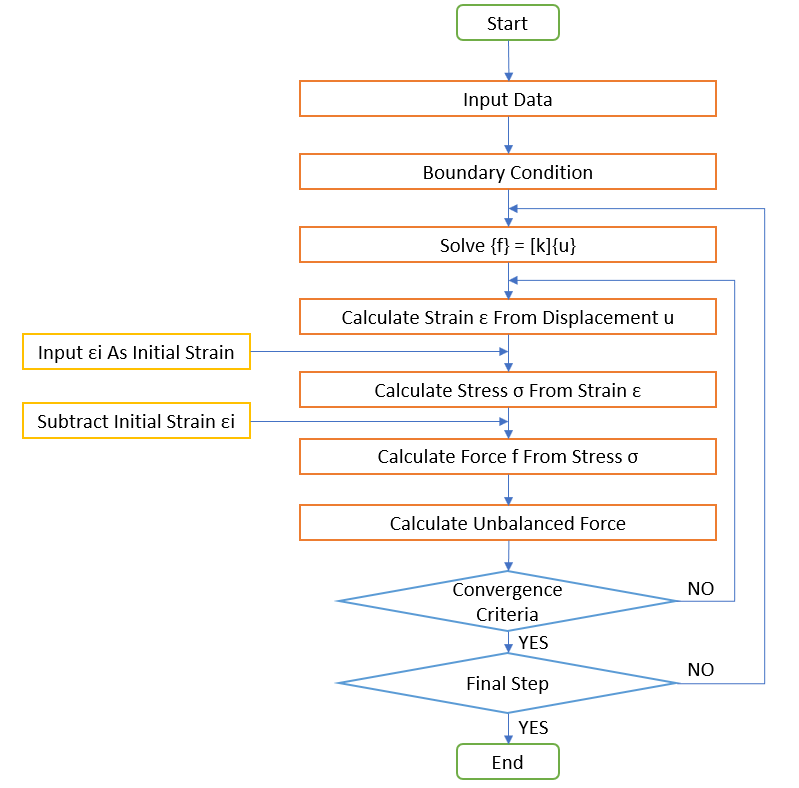
\includegraphics[width=1.0\linewidth]{Files/Method/flow.png}
    \caption{Flow Diagram of Simulation of Expansion Through RBSM}
    \label{fig:Flow}
\end{figure}


For ASR and DEF, the initial strains are introduced at different interfaces in concrete.

Expansion is giving to simulative the behavior of model up to 1.3\% expansion(in one dimensional).

To calculate the one dimensional expansion, here 2 elements located at center of left and right surface, seperately, are selected, their distant before and after expansion is recorded.

\begin{figure}[h!]
\centering
%*******
\begin{subfigure}{.4\textwidth}
  \centering
  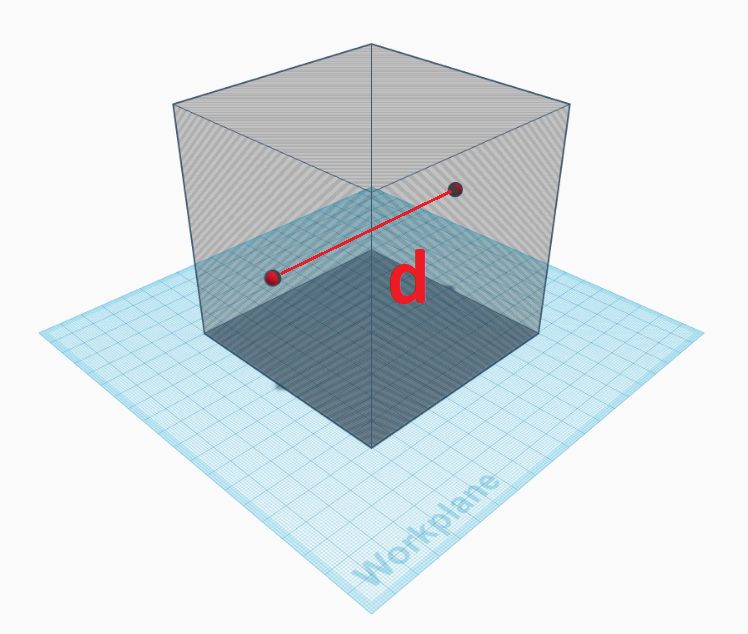
\includegraphics[width=1.0\linewidth]{Files/Method/dis0.png}
\caption{3D View}
\end{subfigure}%
%*******
\begin{subfigure}{.4\textwidth}
  \centering
  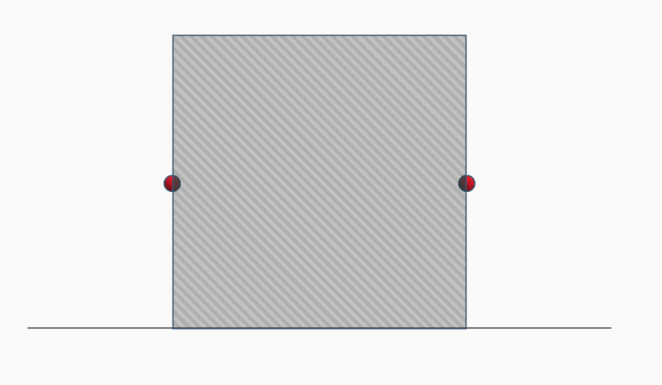
\includegraphics[width=1.0\linewidth]{Files/Method/dis1.png}
\caption{Cross Section View}
\end{subfigure}%
%*******
\caption{Points Selected For Calculation One-dimensional Expansion}
\end{figure}

\subsection{ASR Expansion Behavior In Simulation}

For ASR expansion, the expanse is generated at the location of interfaces between mortar and aggregate. The concept of the initial strain is used here to introduce the expansion.

As we consider the ratio of reactive aggregate may differ the behavior of the model in ASR expansion,  cases of different percentage aggregate expanse are simulated and cross-compared. The reactive aggregates are also chosen randomly.

\begin{figure}
  \centering
  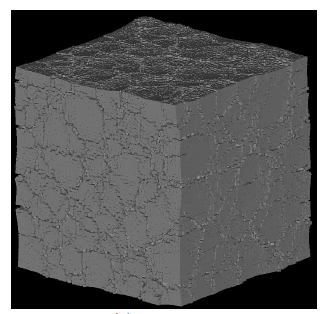
\includegraphics[width=0.4\linewidth]{Files/Background/EDDY_ASR.png}
  \caption{Characteristic Map Cracking Pattern of ASR bu RBSM Simulation, L.EDDY et al. (2016)}
\end{figure}

As in the research done by L.EDDY et al. (2016)\cite{Eddy}, the desired characteristic map cracking pattern of ASR expansion has already achieved in this method. In this simulation, the discussion is focused on the relationship between cracking pattern with aggregate percentage, reactive aggregate, expanding ratio, also the residual mechanical properties of ASR-damaged concrete.

\subsection{DEF Expansion Behavior In Simulation}

Similar model and mechanism are also applied in the simulation of DEF  type expansion. Following the popular theory of expansion in DEF  is caused by expansion of paste, initial strain here is given to the interfaces between mortar elements to present the DEF expansion.

According to the previous study done by L.EDDY et al, simple uniformed paste expansion theory need improvement. Whether for cases giving initial strain to 100\%, 50\% or 25\% random faces of mortar chosen to expanse, the surface of expanded concrete does not match with the actual cracking pattern.

It is well established that high early temperature experienced by the concrete is the most important factor inducing DEF in concrete. (Ghorab et al .,1980\cite{Ghorab}, Heinz, D et al., 1986\ref{Heinz} etc.)

The research done by Anupam (2016)\cite{Awasthi} confirmed the rising of the temperature inside concrete due to combination effect of steam curing and heat of hydration inside the concrete is not uniform. Both the simulation result is done by Astea Macs (FEM based non-linear thermal stress analysis program developed by Research Center of Computational Mechanics, Japan) and the field measurement of temperature rising process inside concrete during steam curing in a concrete plant located in India shows the un-uniformed distribution of maximum temperature experienced. The temperature in the center of the concrete structure is significantly higher than the outer part.

\begin{figure}[ht!]
\centering
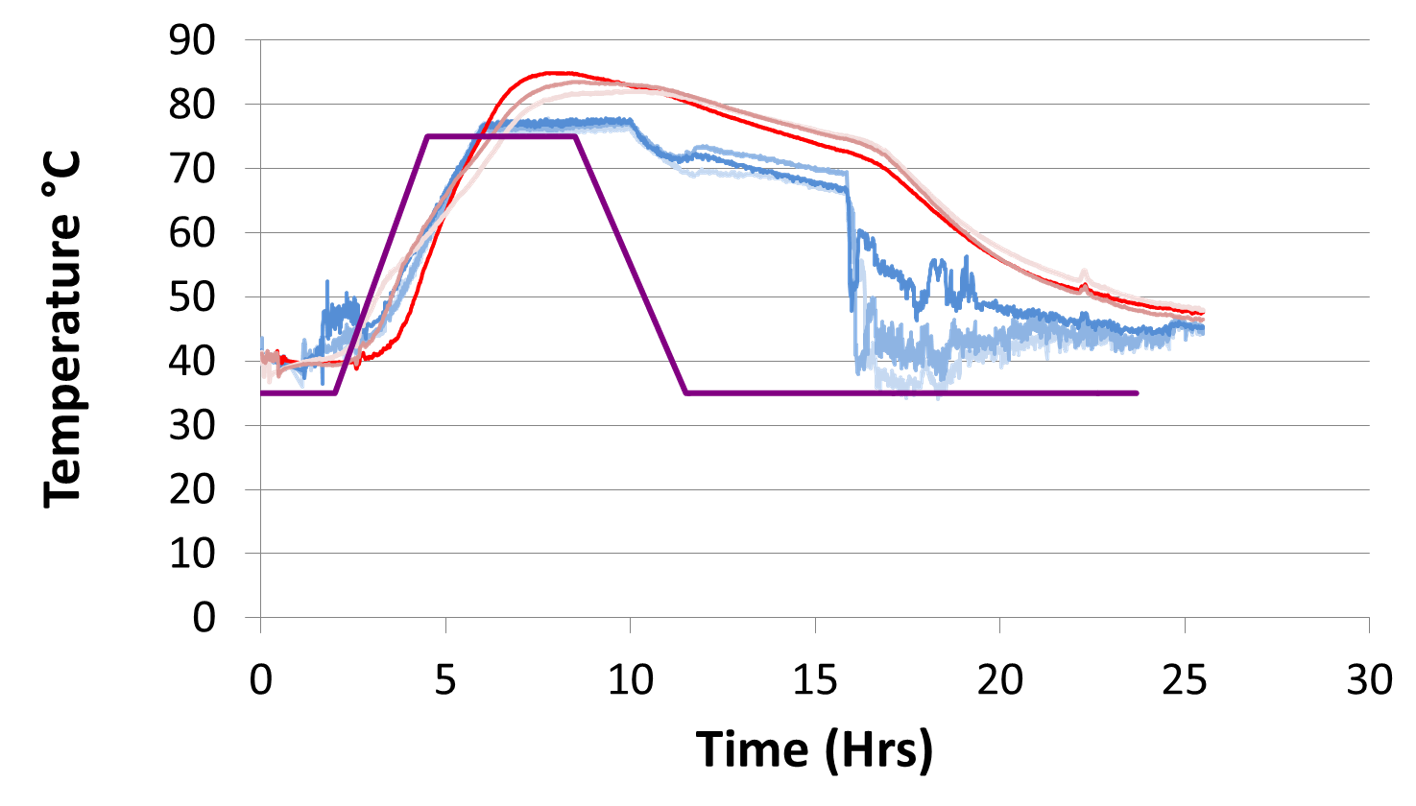
\includegraphics[width=.6\linewidth]{Files/Background/Anupam_2.png}
  \caption{Result of Temperature Measurement, A.AWASTHI 2016}
  \label{fig:temp_measurement}
\end{figure}


The cracking pattern in DEF damaged concrete, recorded by Anupam (2016)\cite{Awasthi}, also suggested the possibility of non-uniformed expansion happens in DEF damaged concrete structure. The cracking concentrated in the outer part of the structure, while the inner part remained undamaged, showing the trend of larger expansion happening in the inner part of the concrete paste.

\begin{figure}[ht!]
\centering
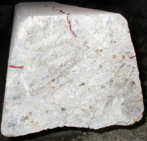
\includegraphics[width=.4\linewidth]{Files/Background/Anupam_5.png}
  \caption{Section View of DEF Damaged Concrete Sleeper, A.AWASTHI 2016}
  \label{fig:section_view}
\end{figure}

Considering the effect of temperature on triggering  DEF expansion and its characteristic cracking pattern, for DEF simulation, uniform expansion does not quite fit with the real situation. The expansion inside concrete structure supposes to be much severe than the outer part. For which here in this research non-uniformed expanding is introduced by giving a different amount of DEF initial strain considering the location of element.


The inner part of the model will be giving larger initial strain,  present the higher maximum temperature experienced, while the outer part mortar will be giving small or none initial strain.

\begin{figure}[ht]
\centering
    %*******
    \begin{subfigure}{.33\textwidth}
      \centering
      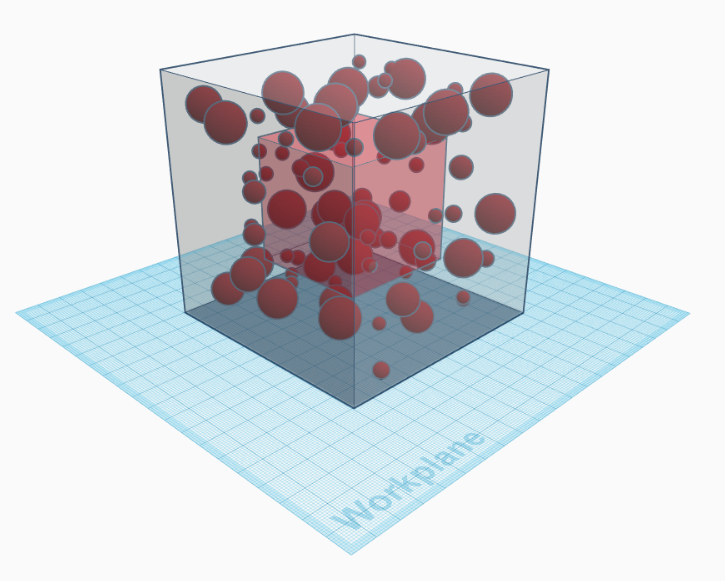
\includegraphics[width=.8\linewidth]{Files/DEF_X/X0_3d.png}
    \end{subfigure}%
    %*******
    \begin{subfigure}{.33\textwidth}
      \centering
      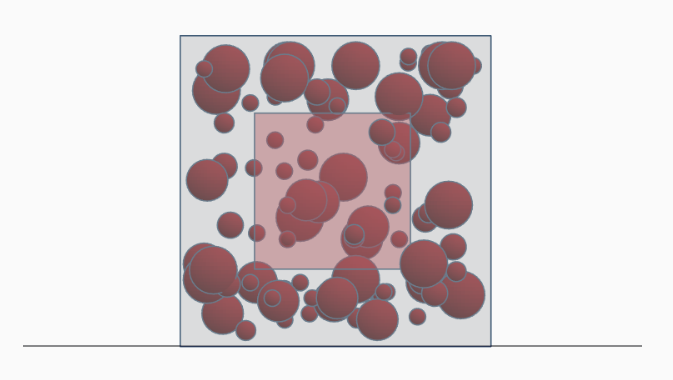
\includegraphics[width=.8\linewidth]{Files/DEF_X/X0_3ds.png}
    \end{subfigure}
    %*******
  \caption{50x50x50mm DEF intensified part range}
  \label{fig:non-uniform DEF}
  \end{figure}


%*******10********20********30********40********50********60********70********80
 % \section{Expansion Model}

\section{Details of Numerical Models for ASR Simulation}

\subsection{Geometry of Numerical Models}

Figure \ref{fig:model} shows the geometry of the model, which is in dimension of 100 x 100 x 100mm. Numbers of elements around 120000. Average diameter of meshed element is around 2mm.

\begin{figure}[ht!]
\centering
\begin{subfigure}{.5\textwidth}
  \centering
  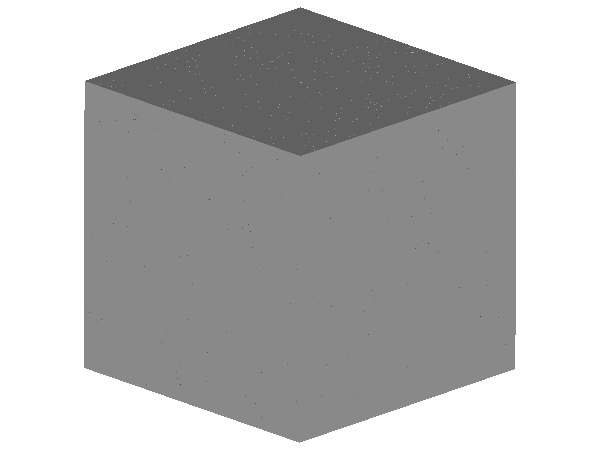
\includegraphics[width=.6\linewidth]{Files/exp_3D/Undamaged.png}
  \caption{3D model in dimension 100x100x100mm}
\end{subfigure}%
\begin{subfigure}{.5\textwidth}
  \centering
  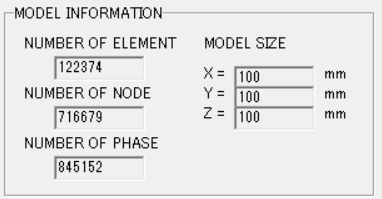
\includegraphics[width=.8\linewidth]{Files/Model/A30.png}
  \caption{Model Detail for 30\% Coarse Aggregate Case}
\end{subfigure}
\caption{Numerical Model for Expanding Simulation}
\label{fig:model}
\end{figure}

\subsection{Coarse Aggregate of Numerical Models}

To analysis the behavior of concrete with different coarse aggregate volume ratio, 15\% coarse aggregate model(Figure \ref{fig:A15_model}) and 30\% coarse aggregate model(Figure \ref{fig:A30_model}) are built for simulation.

\begin{figure}[ht!]
\centering
\begin{subfigure}{.5\textwidth}
  \centering
  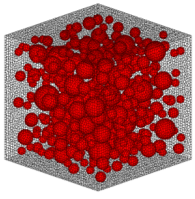
\includegraphics[width=.4\linewidth]{Files/Aggregate/A15.png}
  \caption{15\% Coarse Aggregate}
  \label{fig:A15_model}
\end{subfigure}%
\begin{subfigure}{.5\textwidth}
  \centering
  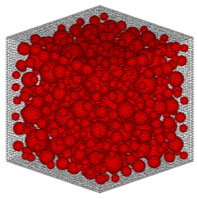
\includegraphics[width=.4\linewidth]{Files/Aggregate/A30.png}
  \caption{30\% Coarse Aggregate}
  \label{fig:A30_model}
\end{subfigure}
\caption{Coarse Aggregate Percentage}
\label{fig:Aggregate_Percentage}
\end{figure}

\subsection{ASR Reactive Coarse Aggregate Ratio}

To analysis the behavior of concrete with different ASR reactive coarse aggregate ratio, 25\% ASR reactive coarse aggregate ratio model and 25\% ASR reactive coarse aggregate ratio model are built for 30\% aggregate case.

\begin{figure}[!h]
\centering
\begin{subfigure}{.5\textwidth}
  \centering
  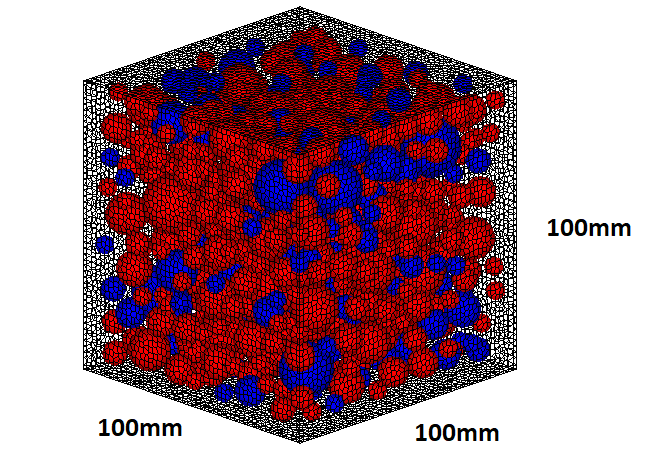
\includegraphics[width=.5\linewidth]{Files/Aggregate/A30P75.png}
  \caption{30\% Coarse Aggregate with 75\% ASR Reactive Aggregate}
\end{subfigure}%
\begin{subfigure}{.5\textwidth}
  \centering
  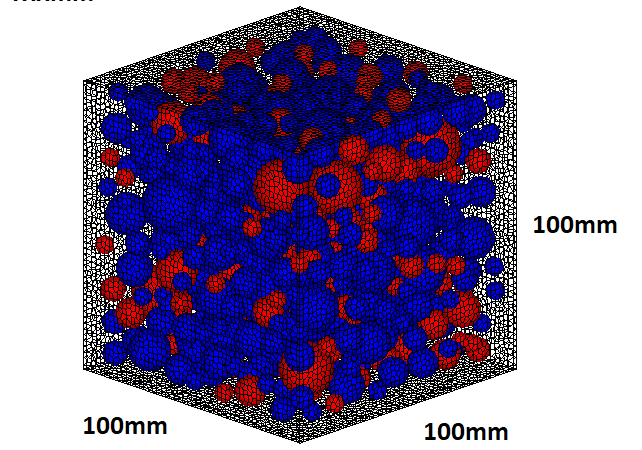
\includegraphics[width=.5\linewidth]{Files/Aggregate/A30P25.png}
  \caption{30\% Coarse Aggregate with 25\% ASR Reactive Aggregate}
\end{subfigure}
\caption{25\% and 75\% ASR Reactive Aggregate Ratio Model}
\label{fig:Aggregate_Percentage}
\end{figure}

\subsection{Boundary Conditions}

\subsubsection{Boundary Condition During ASR Expansion}

During ASR Expansion, no confinements are added to the boundary elements. Models expanse freely in all directions.

\subsubsection{Boundary Conditions During Uni-axial Loading Test}

Figure \ref{boundary} shows the boundary condition of simulation models for uni-axial loading test.

\begin{figure}[h!]
  \centering
  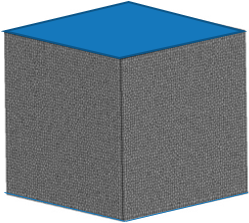
\includegraphics{Files/Background/LOAD.png}
  \caption{Top and Bottom Boundary in Loading}
  \label{boundary}
\end{figure}

In the case of fixed boundary condition, displacement in all directions are assumed as 0 at the bottom. Displacement in horizontal directions are all assumed as 0 at the top, and displacement in vertical direction is increased by 0.02mm downward at each loading step.

In the case of free boundary condition, all boundary elements able to move freely in horizontal direction except 2 center elements in top and bottom are fixed in horizontal direction, to prevent the sliding of whole model during loading. Same as fixed boundary condition cases, displacement in vertical direction is increased by 0.02mm downward at each loading step for top boundary elements.

Loading is applied until the maximum compressive strength is reached.

\subsection{Initial Strain Given For ASR Expansion}

To analysis the relationship of concrete behavior and mechanical properties with expansion amount, initial strain is given between reactive aggregate and mortar.

\begin{table}[ht!]
\centering
\begin{tabular}{ ||p{2cm}|p{2cm}|p{2cm}|p{2cm}|p{2cm}|| }
 \hline
 Aggregate Ratio[\%] &  Reactive Aggregate Ratio[\%] & Boundary Condition & Initial Strain (Each Step) & Expanding Steps \\ [0.5ex]
 \hline\hline
 15 & 11.25 & Fix & 0 & 0 \\
 15 & 11.25 & Fix & 0.0002 & 20 \\
 15 & 11.25 & Fix & 0.0005 & 20 \\
 15 & 11.25 & Fix & 0.001 & 20 \\
 15 & 11.25 & Fix & 0.002 & 20 \\
 15 & 11.25 & Fix & 0.003 & 20 \\

 15 & 11.25 & Free & 0 & 0 \\
 15 & 11.25 & Free & 0.0002 & 20 \\
 15 & 11.25 & Free & 0.0005 & 20 \\
 15 & 11.25 & Free & 0.001 & 20 \\
 15 & 11.25 & Free & 0.002 & 20 \\

 30 & 22.50 & Fix & 0 & 0 \\
 30 & 22.50 & Fix & 0.0002 & 20 \\
 30 & 22.50 & Fix & 0.0005 & 20 \\
 30 & 22.50 & Fix & 0.001 & 20 \\
 30 & 22.50 & Fix & 0.002 & 20 \\
 30 & 22.50 & Fix & 0.003 & 20 \\

 30 & 22.50 & Free & 0 & 0 \\
 30 & 22.50 & Free & 0.0002 & 20 \\
 30 & 22.50 & Free & 0.0005 & 20 \\
 30 & 22.50 & Free & 0.001 & 20 \\
 30 & 22.50 & Free & 0.002 & 20 \\

 30 & 7.50 & Fix & 0 & 0 \\
 30 & 7.50 & Fix & 0.001 & 20 \\
 30 & 7.50 & Fix & 0.002 & 20 \\
 30 & 7.50 & Fix & 0.004 & 20 \\
 30 & 7.50 & Fix & 0.006 & 20 \\  [0.5ex]
 \hline
\end{tabular}
\caption{ASR Models}
\label{table:ASR_MODELS}
\end{table}

%*******10********20********30********40********50********60********70********80
 % \section{Details of Numerical Models for ASR Simulation}

\clearpage
\section{Details of Numerical Models for DEF Simulation}

\subsection{Introduction}

The exactly same model is used for DEF simulation in order to cross compare the cracking patterns and mechanical properties changes under ASR and DEF expansion.

\subsection{Geometry of Numerical Models}

The geometry of the models is exactly the same as models using in ASR simulation, which is in dimension of $100 \times 100 \times 100$ mm.

All materials properties are set to be exactly the same.

\subsection{Coarse Aggregate of Numerical Models}

To analysis the behavior of concrete with different coarse aggregate volume ratio, 15\% coarse aggregate model and 30\% coarse aggregate model (Figure \ref{skjdfhlk}) are built for simulation.

\begin{figure}[!h]
\centering
\begin{subfigure}{.5\textwidth}
  \centering
  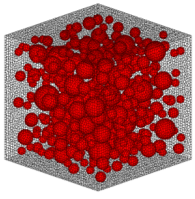
\includegraphics[width=.6\linewidth]{Files/Aggregate/A15.png}
  \caption{15\% Coarse Aggregate}

\end{subfigure}%
\begin{subfigure}{.5\textwidth}
  \centering
  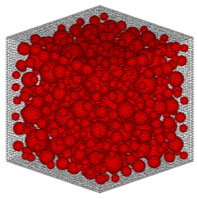
\includegraphics[width=.6\linewidth]{Files/Aggregate/A30.png}
  \caption{30\% Coarse Aggregate}
\end{subfigure}

\caption{Coarse Aggregate Percentage}
\label{skjdfhlk}
\end{figure}

\subsection{DEF Intensified Expansion Area of Numerical Models}

Since DEF is closely related to higher curing temperature, here we choose to intensified the expansion in center part of model.

Here we chooses 3 cases in different expansion intensified area. The Table \ref{table:DEF_X} is a list of cases simulated, illustration is presented in Figure \ref{fig:DEFffff_X}.

\begin{table}[ht!]
  \caption{DEF Intensified Expansion Area}
\centering
\begin{tabular}{||c c c||}
 \hline
 Case &  Expansion Intensified Depth[mm] &  Expansion Intensified Zone \\ [0.5ex]
 \hline\hline
 1 & 0 & $100 \times 100 \times 100$ mm \\
 2 & 12.5 & $75 \times 75 \times 75$ mm \\
 3 & 25 & $50 \times 50 \times 50$ mm \\ [0.5ex]
 \hline
\end{tabular}

\label{table:DEF_X}
\end{table}

\begin{figure}[ht]
\centering
    %*******
    \begin{subfigure}{.33\textwidth}
      \centering
      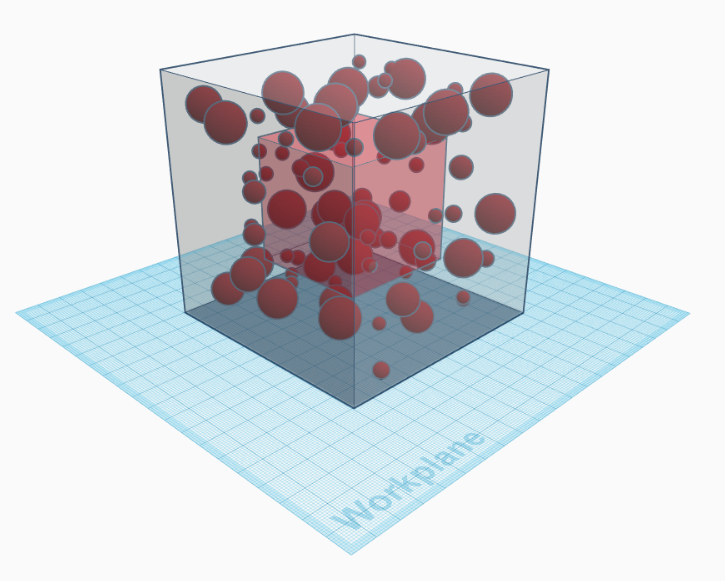
\includegraphics[width=.8\linewidth]{Files/DEF_X/X0_3d.png}
      \caption{Intensified  \\ $50 \times 50 \times 50$ mm Case}
    \end{subfigure}%
    %*******
    \begin{subfigure}{.33\textwidth}
      \centering
      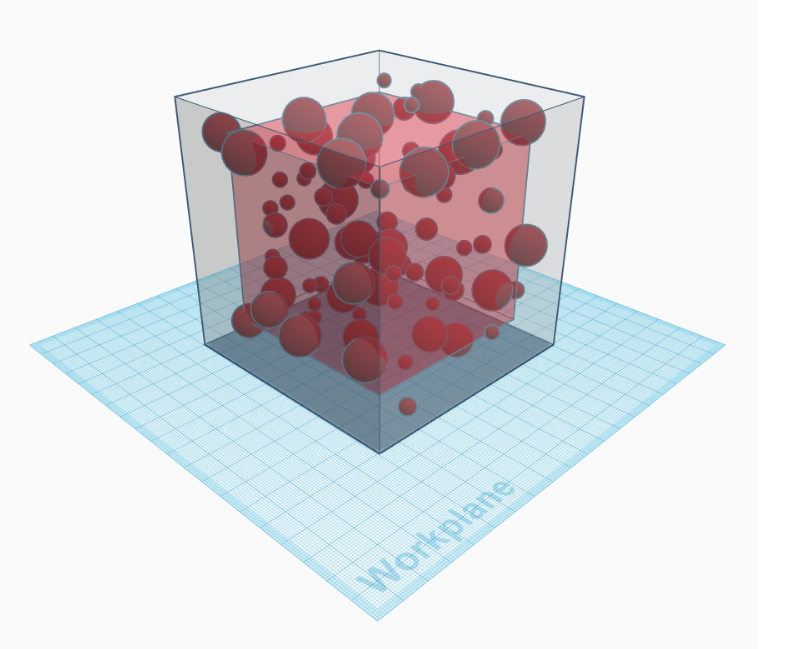
\includegraphics[width=.8\linewidth]{Files/DEF_X/X-5_3d.png}
      \caption{Intensified  \\ $75 \times 75 \times 75$ mm Case}
    \end{subfigure}%
    %*******
    \begin{subfigure}{.33\textwidth}
      \centering
      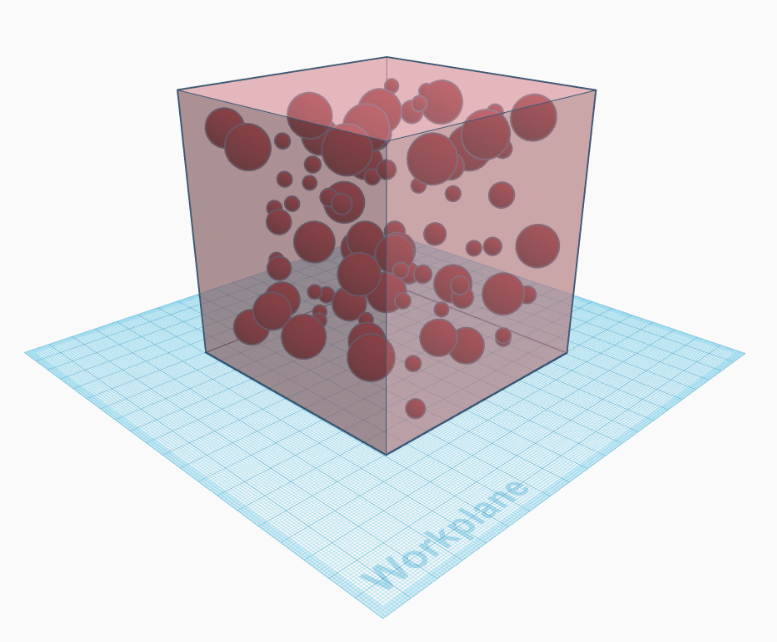
\includegraphics[width=.8\linewidth]{Files/DEF_X/X-1_3d.png}
      \caption{Intensified  \\ $100 \times 100 \times 100$ mm Case}
    \end{subfigure}
    %*******
    %*******
    \begin{subfigure}{.33\textwidth}
      \centering
      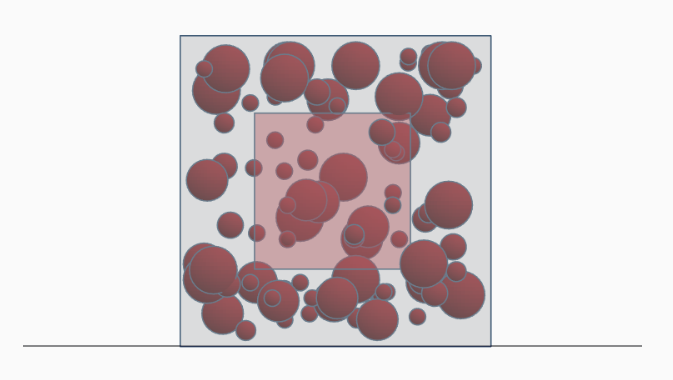
\includegraphics[width=.8\linewidth]{Files/DEF_X/X0_3ds.png}
      \caption{Intensified  \\ $50 \times 50 \times 50$ mm Case\\ Cross Section}
    \end{subfigure}%
    %*******
    \begin{subfigure}{.33\textwidth}
      \centering
      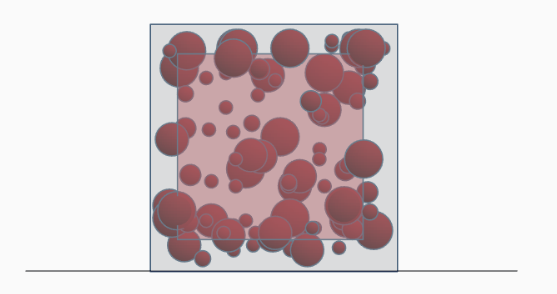
\includegraphics[width=.8\linewidth]{Files/DEF_X/X-5_3ds.png}
      \caption{Intensified \\  $75 \times 75 \times 75$ mm Case \\ Cross Section}
    \end{subfigure}%
    %*******
    \begin{subfigure}{.33\textwidth}
      \centering
      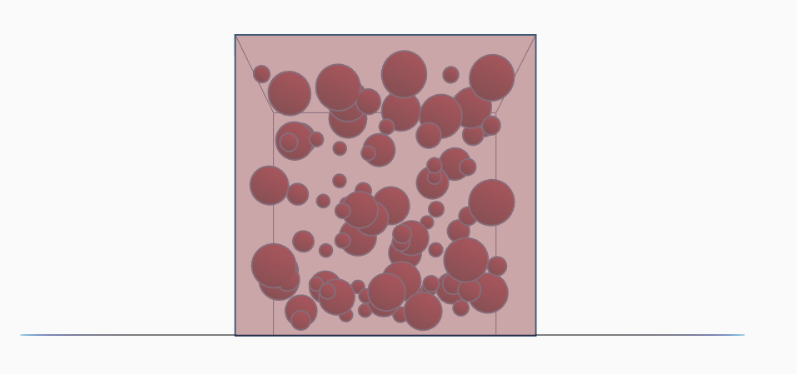
\includegraphics[width=.9\linewidth]{Files/DEF_X/X-1_3ds.png}
      \caption{Intensified  \\ $100 \times 100 \times 100$ mm Case\\ Cross Section}
    \end{subfigure}
    %*******
  \caption{DEF intensified part range}
  \label{fig:DEFffff_X}
\end{figure}

\subsection{Boundary Conditions}

\subsubsection{Boundary Condition During DEF Expansion}

Same as in ASR expansion, during DEF expansion, no confinements are added to the boundary elements. Models expanse freely in all directions.

\subsubsection{Boundary Conditions During Uni-axial Loading Test}

Same as in ASR expansion, Uni-axial Loading Test is applied with both fixed and free boundary conditions(Figure \ref{boundaaary}).

\begin{figure}[h!]
  \centering
  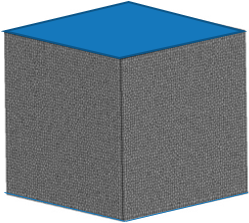
\includegraphics{Files/Background/LOAD.png}
  \caption{Top and Bottom Boundary in Loading}
  \label{boundaaary}
\end{figure}

In the case of fixed boundary condition, displacement in all directions are assumed as 0 at the bottom. Displacement in horizontal directions are all assumed as 0 at the top, and displacement in vertical direction is increased by 0.02 mm downward at each loading step.

In the case of free boundary condition, all boundary elements able to move freely in horizontal direction except 2 center elements in top and bottom are fixed in horizontal direction, to prevent the sliding of whole model during loading. Same as fixed boundary condition cases, displacement in vertical direction is increased by 0.02 mm downward at each loading step for top boundary elements.

Loading is applied until the maximum compressive strength is reached.
 % \section{Details of Numerical Models for DEF Simulation}


\section{Conclusions}

In this chapter describe about the numerical simulation system that has been used in this research, RBSM. In the this study, RBSM is used to simulate the deterioration of concrete due to expansion such as expansion crack, then the mechanical properties of expanded concrete will be calculated by using RBSM.

In RBSM, the response of normal spring and shear spring represent the mechanical response of mortar and aggregate member. By giving initial strain, the response of spring changed in the relatively close manner as real expanded structure. Also the cases that will be simulated in later are introduced in this chapter. The details of simulation results from this simulation will be described again in Chapter 3 and 4.
 

 %*******10********20********30********40********50********60********70********80

\chap{Simulation of Cracking Pattern Of ASR and DEF Expanded Concrete}

%*******10********20********30********40********50********60********70********80

\section{General}

In this chapter, three-dimensional expanded simulations are carried out on concrete models in free condition. The purpose of this study is for the prediction of the behavior during the expansion of concrete, especially the cracking pattern and stress distribution.

\section{Cracking Pattern caused by Pure ASR Expansion}

\subsection{ASR Expansion Simulation of Single Aggregate Case}

In this section, simulation of ASR expansion on a single aggregate case in size only $10 \times 10 \times 10$ mm is presented(Figure \ref{smallasr}).

Since this model is very small and simple, it is easier to analyze the behavior of ASR expansion in very small scale around coarse aggregate.

The expanse is generated at the location of interfaces between mortar and aggregate, to introduce the expansion, as introduced in chapter 2.

%TODO: Single Aggregate 3D, 2D

\begin{figure}[h!]
\centering
%*******
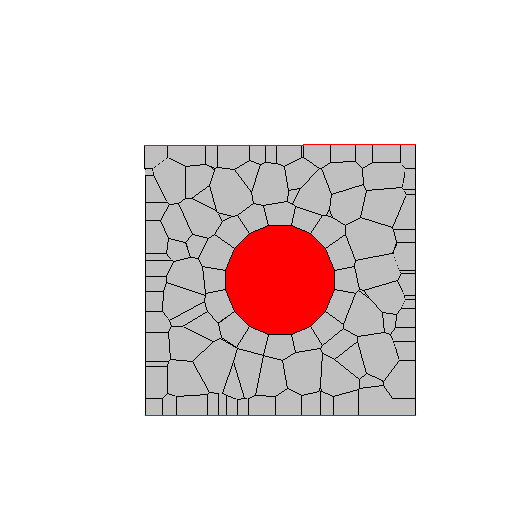
\includegraphics[width=0.4\linewidth]{Files/Small_ASR/CR/DEP5-STEP(001).png}
\caption{Single Aggregate Case in Size $10 \times 10 \times 10$ mm}
\label{smallasr}
\end{figure}

0.001 initial strain is introduced in each step at the interfaces between the aggregate and paste elements. Totally 20 steps of expansion are done.

% Small ASR CR
  \begin{figure}[ht!]
  \centering
      %*******
      \begin{subfigure}{.25\textwidth}
        \centering
        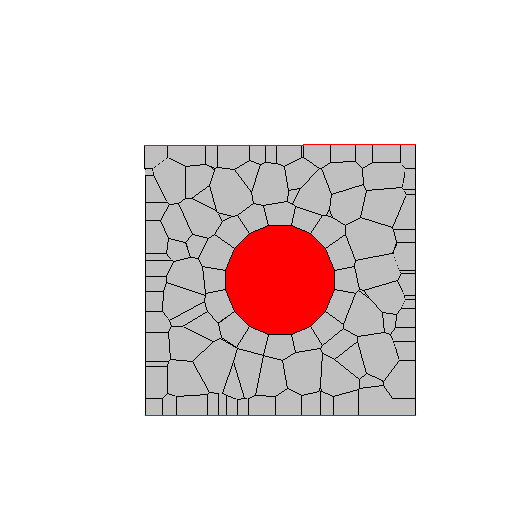
\includegraphics[width=1.0\linewidth]{Files/Small_ASR/CR/DEP5-STEP(001).png}
      \caption{Step 1}
      \end{subfigure}%
      %*******
      \begin{subfigure}{.25\textwidth}
        \centering
        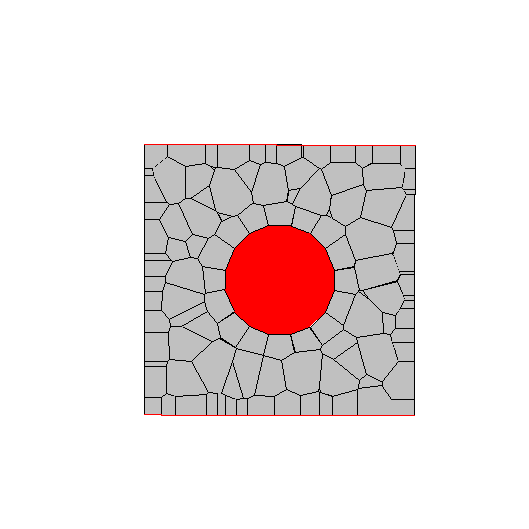
\includegraphics[width=1.0\linewidth]{Files/Small_ASR/CR/DEP5-STEP(002).png}
      \caption{Step 2}
      \end{subfigure}%
      %*******
      \begin{subfigure}{.25\textwidth}
        \centering
        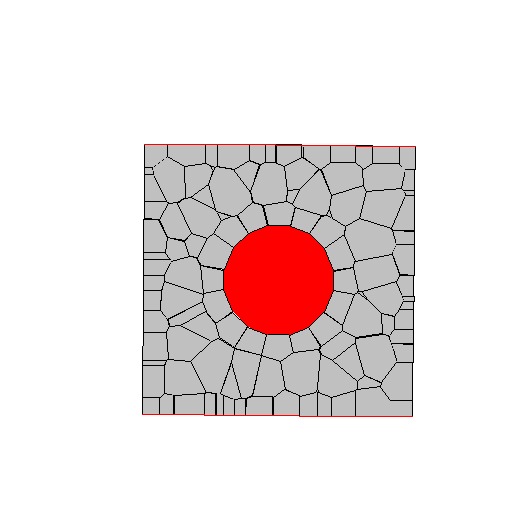
\includegraphics[width=1.0\linewidth]{Files/Small_ASR/CR/DEP5-STEP(003).png}
      \caption{Step 3}
      \end{subfigure}%
      %*******
      \begin{subfigure}{.25\textwidth}
        \centering
        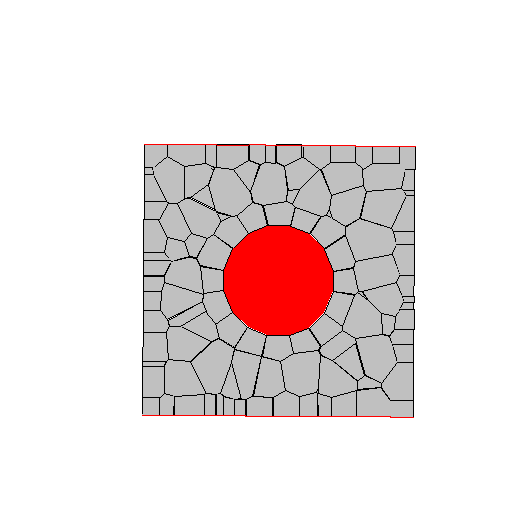
\includegraphics[width=1.0\linewidth]{Files/Small_ASR/CR/DEP5-STEP(004).png}
      \caption{Step 4}
      \end{subfigure}

      %*******
      %*******
      \begin{subfigure}{.25\textwidth}
        \centering
        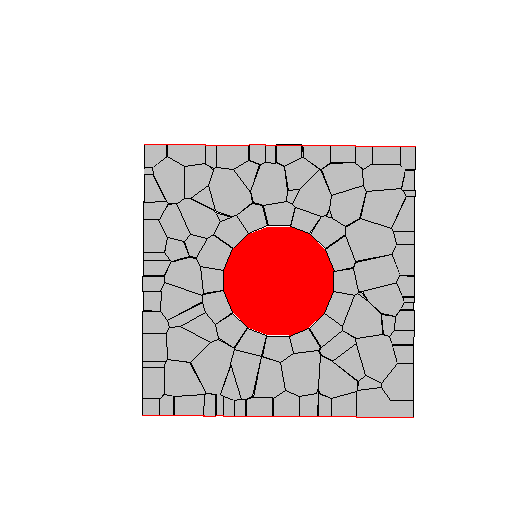
\includegraphics[width=1.0\linewidth]{Files/Small_ASR/CR/DEP5-STEP(005).png}
      \caption{Step 5}
      \end{subfigure}%
      %*******
      \begin{subfigure}{.25\textwidth}
        \centering
        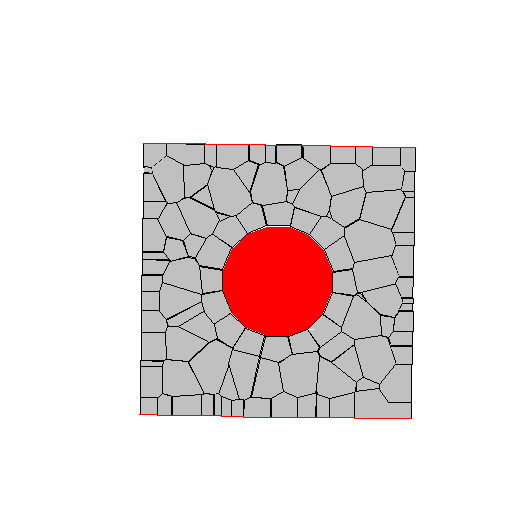
\includegraphics[width=1.0\linewidth]{Files/Small_ASR/CR/DEP5-STEP(006).png}
      \caption{Step 6}
      \end{subfigure}%
      %*******
      \begin{subfigure}{.25\textwidth}
        \centering
        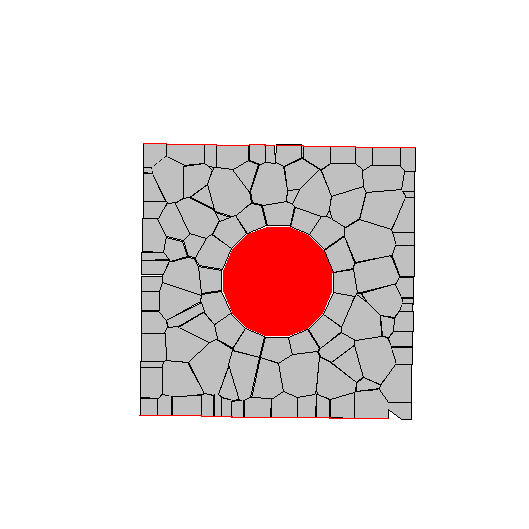
\includegraphics[width=1.0\linewidth]{Files/Small_ASR/CR/DEP5-STEP(007).png}
      \caption{Step 7}
      \end{subfigure}%
      %*******
      \begin{subfigure}{.25\textwidth}
        \centering
        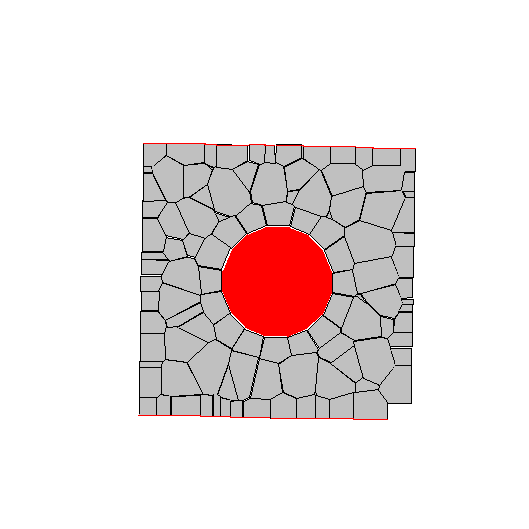
\includegraphics[width=1.0\linewidth]{Files/Small_ASR/CR/DEP5-STEP(008).png}
      \caption{Step 4}
      \end{subfigure}

      %*******
      %*******
      \begin{subfigure}{.25\textwidth}
        \centering
        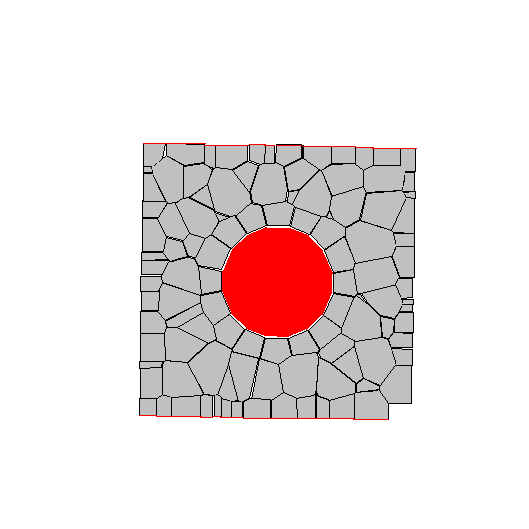
\includegraphics[width=1.0\linewidth]{Files/Small_ASR/CR/DEP5-STEP(009).png}
      \caption{Step 9}
      \end{subfigure}%
      %*******
      \begin{subfigure}{.25\textwidth}
        \centering
        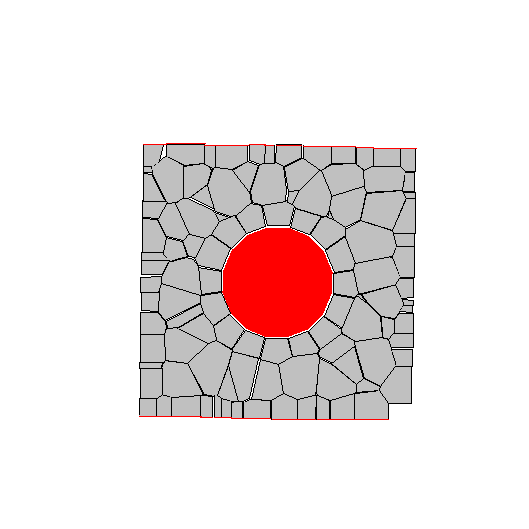
\includegraphics[width=1.0\linewidth]{Files/Small_ASR/CR/DEP5-STEP(010).png}
      \caption{Step 10}
      \end{subfigure}%
      %*******
      \begin{subfigure}{.25\textwidth}
        \centering
        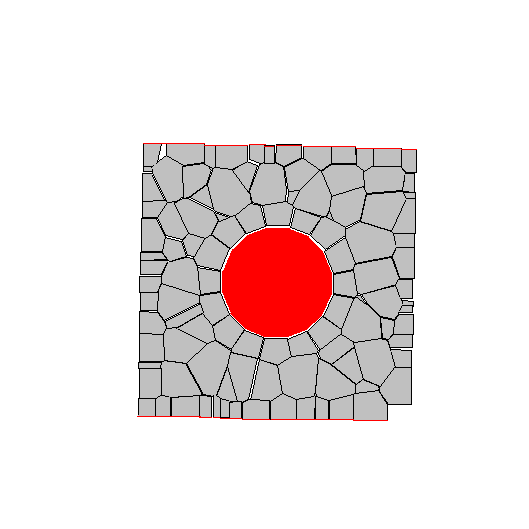
\includegraphics[width=1.0\linewidth]{Files/Small_ASR/CR/DEP5-STEP(011).png}
      \caption{Step 11}
      \end{subfigure}%
      %*******
      \begin{subfigure}{.25\textwidth}
        \centering
        \includegraphics[width=1.0\linewidth]{Files/Small_ASR/CR/DEP5-STEP(012).png}
      \caption{Step 12}
      \end{subfigure}

      %*******
      %*******
      \begin{subfigure}{.25\textwidth}
        \centering
        \includegraphics[width=1.0\linewidth]{Files/Small_ASR/CR/DEP5-STEP(013).png}
      \caption{Step 13}
      \end{subfigure}%
      %*******
      \begin{subfigure}{.25\textwidth}
        \centering
        \includegraphics[width=1.0\linewidth]{Files/Small_ASR/CR/DEP5-STEP(014).png}
      \caption{Step 14}
      \end{subfigure}%
      %*******
      \begin{subfigure}{.25\textwidth}
        \centering
        \includegraphics[width=1.0\linewidth]{Files/Small_ASR/CR/DEP5-STEP(015).png}
      \caption{Step 15}
      \end{subfigure}%
      %*******
      \begin{subfigure}{.25\textwidth}
        \centering
        \includegraphics[width=1.0\linewidth]{Files/Small_ASR/CR/DEP5-STEP(016).png}
      \caption{Step 16}
      \end{subfigure}

      %*******
      %*******
      \begin{subfigure}{.25\textwidth}
        \centering
        \includegraphics[width=1.0\linewidth]{Files/Small_ASR/CR/DEP5-STEP(017).png}
      \caption{Step 17}
      \end{subfigure}%
      %*******
      \begin{subfigure}{.25\textwidth}
        \centering
        \includegraphics[width=1.0\linewidth]{Files/Small_ASR/CR/DEP5-STEP(018).png}
      \caption{Step 18}
      \end{subfigure}%
      %*******
      \begin{subfigure}{.25\textwidth}
        \centering
        \includegraphics[width=1.0\linewidth]{Files/Small_ASR/CR/DEP5-STEP(019).png}
      \caption{Step 19}
      \end{subfigure}%
      %*******
      \begin{subfigure}{.25\textwidth}
        \centering
        \includegraphics[width=1.0\linewidth]{Files/Small_ASR/CR/DEP5-STEP(020).png}
      \caption{Step 20}
      \end{subfigure}

      \begin{subfigure}{0.8\textwidth}
  \includegraphics[width=0.8\linewidth]{Files/exp_3D/tag_crack_s.png}
\end{subfigure}%


  \caption{Cross Section in Each Step for ASR $10 \times 10 \times 10$ mm Case ($Deformation \times 10$)}
  \label{fig:ASR_Small_ASR_CR}
  \end{figure}


From the Figure \ref{fig:ASR_Small_ASR_CR}, we can see that step by step with initial stain introducing into the model, distance appears between aggregate and the surrounding element at first, which theoretically should be filled by ASR gel, the product of ASR reaction.

After, by the influence of the unbalanced force start from the aggregate-mortar interfaces, elements surround it also react. Cracks start to generate from aggregate to the paste surrounding it.

The total volume of this small model is increasing step by step, while until the step 20 the model expanded 0.1625\% one dimensionally.

% Small ASR IS
  \begin{figure}[ht!]
  \centering
      %*******
      \begin{subfigure}{.25\textwidth}
        \centering
        \includegraphics[width=1.0\linewidth]{Files/Small_ASR/IS/DEP5-STEP(001).png}
      \caption{Step 1}
      \end{subfigure}%
      %*******
      \begin{subfigure}{.25\textwidth}
        \centering
        \includegraphics[width=1.0\linewidth]{Files/Small_ASR/IS/DEP5-STEP(002).png}
      \caption{Step 2}
      \end{subfigure}%
      %*******
      \begin{subfigure}{.25\textwidth}
        \centering
        \includegraphics[width=1.0\linewidth]{Files/Small_ASR/IS/DEP5-STEP(003).png}
      \caption{Step 3}
      \end{subfigure}%
      %*******
      \begin{subfigure}{.25\textwidth}
        \centering
        \includegraphics[width=1.0\linewidth]{Files/Small_ASR/IS/DEP5-STEP(004).png}
      \caption{Step 4}
      \end{subfigure}

      %*******
      %*******
      \begin{subfigure}{.25\textwidth}
        \centering
        \includegraphics[width=1.0\linewidth]{Files/Small_ASR/IS/DEP5-STEP(005).png}
      \caption{Step 5}
      \end{subfigure}%
      %*******
      \begin{subfigure}{.25\textwidth}
        \centering
        \includegraphics[width=1.0\linewidth]{Files/Small_ASR/IS/DEP5-STEP(006).png}
      \caption{Step 6}
      \end{subfigure}%
      %*******
      \begin{subfigure}{.25\textwidth}
        \centering
        \includegraphics[width=1.0\linewidth]{Files/Small_ASR/IS/DEP5-STEP(007).png}
      \caption{Step 7}
      \end{subfigure}%
      %*******
      \begin{subfigure}{.25\textwidth}
        \centering
        \includegraphics[width=1.0\linewidth]{Files/Small_ASR/IS/DEP5-STEP(008).png}
      \caption{Step 4}
      \end{subfigure}

      %*******
      %*******
      \begin{subfigure}{.25\textwidth}
        \centering
        \includegraphics[width=1.0\linewidth]{Files/Small_ASR/IS/DEP5-STEP(009).png}
      \caption{Step 9}
      \end{subfigure}%
      %*******
      \begin{subfigure}{.25\textwidth}
        \centering
        \includegraphics[width=1.0\linewidth]{Files/Small_ASR/IS/DEP5-STEP(010).png}
      \caption{Step 10}
      \end{subfigure}%
      %*******
      \begin{subfigure}{.25\textwidth}
        \centering
        \includegraphics[width=1.0\linewidth]{Files/Small_ASR/IS/DEP5-STEP(011).png}
      \caption{Step 11}
      \end{subfigure}%
      %*******
      \begin{subfigure}{.25\textwidth}
        \centering
        \includegraphics[width=1.0\linewidth]{Files/Small_ASR/IS/DEP5-STEP(012).png}
      \caption{Step 12}
      \end{subfigure}

      %*******
      %*******
      \begin{subfigure}{.25\textwidth}
        \centering
        \includegraphics[width=1.0\linewidth]{Files/Small_ASR/IS/DEP5-STEP(013).png}
      \caption{Step 13}
      \end{subfigure}%
      %*******
      \begin{subfigure}{.25\textwidth}
        \centering
        \includegraphics[width=1.0\linewidth]{Files/Small_ASR/IS/DEP5-STEP(014).png}
      \caption{Step 14}
      \end{subfigure}%
      %*******
      \begin{subfigure}{.25\textwidth}
        \centering
        \includegraphics[width=1.0\linewidth]{Files/Small_ASR/IS/DEP5-STEP(015).png}
      \caption{Step 15}
      \end{subfigure}%
      %*******
      \begin{subfigure}{.25\textwidth}
        \centering
        \includegraphics[width=1.0\linewidth]{Files/Small_ASR/IS/DEP5-STEP(016).png}
      \caption{Step 16}
      \end{subfigure}

      %*******
      %*******
      \begin{subfigure}{.25\textwidth}
        \centering
        \includegraphics[width=1.0\linewidth]{Files/Small_ASR/IS/DEP5-STEP(017).png}
      \caption{Step 17}
      \end{subfigure}%
      %*******
      \begin{subfigure}{.25\textwidth}
        \centering
        \includegraphics[width=1.0\linewidth]{Files/Small_ASR/IS/DEP5-STEP(018).png}
      \caption{Step 18}
      \end{subfigure}%
      %*******
      \begin{subfigure}{.25\textwidth}
        \centering
        \includegraphics[width=1.0\linewidth]{Files/Small_ASR/IS/DEP5-STEP(019).png}
      \caption{Step 19}
      \end{subfigure}%
      %*******
      \begin{subfigure}{.25\textwidth}
        \centering
        \includegraphics[width=1.0\linewidth]{Files/Small_ASR/IS/DEP5-STEP(020).png}
      \caption{Step 20}
      \end{subfigure}

      \begin{subfigure}{0.8\textwidth}
  \includegraphics[width=0.8\linewidth]{Files/exp_3D/tagCS10s.png}
\end{subfigure}%


  \caption{Internal Stress in Each Step for ASR $10 \times 10 \times 10$ mm Case ($Deformation \times 10$)}
  \label{fig:ASR_Small_ASR_IS}
  \end{figure}


Also, the Inner Stress condition for each step is collected and shown in Figure \ref{fig:ASR_Small_ASR_IS}, which can also reveal many details in the expanding procedure.

From step 1 compressive stress is generated in and one layer around the reactive aggregate, due to the initial strain added to the reactive interfaces. While other paste elements located around reactive aggregate reacted in tension status.

This very small size simple example shows logically our method of adding initial strain to generate ASR expansion should work in the way we assumed.


 %*******10********20********30********40********50********60********70********80
\clearpage
\section{Cracking Pattern caused by Pure ASR Expansion}

%*******10********20********30********40********50********60********70********80

\subsection{Single ASR Expansion Simulation}

%*******10********20********30********40********50********60********70********80
% illustration of A30P75 ASR C D0 A0.001 S20 Expansion

In this section, the process of simulated one ASR expansion is present. The expanse is generated at the location of interfaces between mortar and reactive aggregate, to introduce the expansion, as introduced in chapter 2.

For usually the case not all aggregate inside concrete structure are ASR reactive aggregate, here only partial of aggregates are selected to be ASR reactive and will be givin initial strain in expansion steps to simulate ASR expansion.

This single example case has been choosing here use the model in the dimension of 100x100x100mm, with 30\% aggregate, of which 75\% are ASR reactive. Aggregate in Figure \ref{fig:A30_modelll} in red color is assumed as ASR reactive, while aggregate in blue color is assumed as non-reactive aggregate.

  \begin{figure}[ht!]
  \centering
  \includegraphics[width=.3\linewidth]{Files/Aggregate/A30P75.png}
    \caption{30\% Coarse Aggregate}
    \label{fig:A30_modelll}
  \end{figure}

To simulate ASR expansion, an initial strain of 0.001 is given in each step, for totally 20 steps expansion. Before and after expansion, the distance of element between 2 elements is recorded to gauge the gloal expansion. These two element selected here are the middle element in the left surface of model and the middle element in the left surface of model, as introduced in chapter 2.

%*******10********20********30********40********50********60********70********80

% illustration of A30P75 ASR C D0 A0.001 S20 Expansion

  \begin{table}[ht]
  \centering
  \begin{tabular}{ ||p{3cm}|p{3cm}||p{3cm}|p{3cm}|| }
  \hline
   Step &  Expansion & Step & Expansion \\
   \hline\hline
    1 & 0.000136  & 11 & 0.002140 \\
    2 & 0.000314  & 12 & 0.002358 \\
    3 & 0.000501  & 13 & 0.002582 \\
    4 & 0.000695  & 14 & 0.002812 \\
    5 & 0.000894  & 15 & 0.003049 \\
    6 & 0.001096  & 16 & 0.003278 \\
    7 & 0.001301  & 17 & 0.003536 \\
    8 & 0.001507  & 18 & 0.003767 \\
    9 & 0.001715  & 19 & 0.003989 \\
    10 & 0.001924  & 20  & 0.004223 \\
    \hline
    \end{tabular}
  \caption{Expansion in Each Step for A30 P75 Case 3}
  \label{table:A30P75_3_EXP}
  \end{table}

  \begin{figure}[ht!]
  \centering
  \includegraphics[width=.8\linewidth]{Files/exp_plot/ASRA30P75_3_exp.png}
    \caption{Global Expansion vs. Step}
    \label{fig:ASRA30P75_3_exp}
  \end{figure}

%*******10********20********30********40********50********60********70********80

With the increasing of initial strain giving, the global expansion also gradually increasing. After 20 steps of ASR expansion, the model here reached 0.4223\% expansion(one-dimensionally). Characteristic ASR map cracking pattern can be seen on the surface of the expanded concrete model in Figure \ref{fig:ASR_A30P75_3_3D_1}.

Here the surface cracking from experimental result, done by ALKANA in 2013, is shown in Figure \ref{ALKANASRcrack}, by ALKANA(2013)\cite{ALKANA}, in shape of 100x100x400mm, with 0.10 percent one-dimensional expansion, for comparing. It can be seen that in Figure \ref{fig:ASR_A30P75_3_3D_1}, similar map cracking is represented.

  \begin{figure}[ht!]
  \centering
  \includegraphics[width=.8\linewidth]{Reference/ALKANASRcrack.png}
    \caption{Prismatic specimens of G-C, G-A, and G-B concretes respectively[ALKANA, 2012]}
    \label{ALKANASRcrack}
  \end{figure}


% ASRA30P75_3 Surface Cracking
  \begin{figure}[ht]
  \centering
      %*******
      \begin{subfigure}{.5\textwidth}
        \centering
        \includegraphics[width=.8\linewidth]{Files/exp_3D/ASR/A30P75_3_3d.png}
      \end{subfigure}%
      \begin{subfigure}{.5\textwidth}
        \centering
        \includegraphics[width=.8\linewidth]{Files/exp_3D/ASR/A30P75_3_3ds.png}
        \end{subfigure}
        %*******
    \caption{3D Surface Cracks, 0.4223\% Expansion (Deformation x 10)}
    \label{fig:ASR_A30P75_3_3D_1}
  \end{figure}

% Internal Stress for step 1-20 ASR_A30_P75_3

  \begin{figure}[ht!]
  \centering
      %*******
      \begin{subfigure}{.25\textwidth}
        \centering
        \includegraphics[width=1.0\linewidth]{Files//A30P75_3_IS/DEP50-STEP(001).png}
      \caption{Step 1}
      \end{subfigure}%
      %*******
      \begin{subfigure}{.25\textwidth}
        \centering
        \includegraphics[width=1.0\linewidth]{Files/A30P75_3_IS/DEP50-STEP(002).png}
      \caption{Step 2}
      \end{subfigure}%
      %*******
      \begin{subfigure}{.25\textwidth}
        \centering
        \includegraphics[width=1.0\linewidth]{Files/A30P75_3_IS/DEP50-STEP(003).png}
      \caption{Step 3}
      \end{subfigure}%
      %*******
      \begin{subfigure}{.25\textwidth}
        \centering
        \includegraphics[width=1.0\linewidth]{Files/A30P75_3_IS/DEP50-STEP(004).png}
      \caption{Step 4}
      \end{subfigure}

      %*******
      %*******
      \begin{subfigure}{.25\textwidth}
        \centering
        \includegraphics[width=1.0\linewidth]{Files//A30P75_3_IS/DEP50-STEP(005).png}
      \caption{Step 5}
      \end{subfigure}%
      %*******
      \begin{subfigure}{.25\textwidth}
        \centering
        \includegraphics[width=1.0\linewidth]{Files/A30P75_3_IS/DEP50-STEP(006).png}
      \caption{Step 6}
      \end{subfigure}%
      %*******
      \begin{subfigure}{.25\textwidth}
        \centering
        \includegraphics[width=1.0\linewidth]{Files/A30P75_3_IS/DEP50-STEP(007).png}
      \caption{Step 7}
      \end{subfigure}%
      %*******
      \begin{subfigure}{.25\textwidth}
        \centering
        \includegraphics[width=1.0\linewidth]{Files/A30P75_3_IS/DEP50-STEP(008).png}
      \caption{Step 4}
      \end{subfigure}

      %*******
      %*******
      \begin{subfigure}{.25\textwidth}
        \centering
        \includegraphics[width=1.0\linewidth]{Files//A30P75_3_IS/DEP50-STEP(009).png}
      \caption{Step 9}
      \end{subfigure}%
      %*******
      \begin{subfigure}{.25\textwidth}
        \centering
        \includegraphics[width=1.0\linewidth]{Files/A30P75_3_IS/DEP50-STEP(010).png}
      \caption{Step 10}
      \end{subfigure}%
      %*******
      \begin{subfigure}{.25\textwidth}
        \centering
        \includegraphics[width=1.0\linewidth]{Files/A30P75_3_IS/DEP50-STEP(011).png}
      \caption{Step 11}
      \end{subfigure}%
      %*******
      \begin{subfigure}{.25\textwidth}
        \centering
        \includegraphics[width=1.0\linewidth]{Files/A30P75_3_IS/DEP50-STEP(012).png}
      \caption{Step 12}
      \end{subfigure}

      %*******
      %*******
      \begin{subfigure}{.25\textwidth}
        \centering
        \includegraphics[width=1.0\linewidth]{Files//A30P75_3_IS/DEP50-STEP(013).png}
      \caption{Step 13}
      \end{subfigure}%
      %*******
      \begin{subfigure}{.25\textwidth}
        \centering
        \includegraphics[width=1.0\linewidth]{Files/A30P75_3_IS/DEP50-STEP(014).png}
      \caption{Step 14}
      \end{subfigure}%
      %*******
      \begin{subfigure}{.25\textwidth}
        \centering
        \includegraphics[width=1.0\linewidth]{Files/A30P75_3_IS/DEP50-STEP(015).png}
      \caption{Step 15}
      \end{subfigure}%
      %*******
      \begin{subfigure}{.25\textwidth}
        \centering
        \includegraphics[width=1.0\linewidth]{Files/A30P75_3_IS/DEP50-STEP(016).png}
      \caption{Step 16}
      \end{subfigure}

      %*******
      %*******
      \begin{subfigure}{.25\textwidth}
        \centering
        \includegraphics[width=1.0\linewidth]{Files//A30P75_3_IS/DEP50-STEP(017).png}
      \caption{Step 17}
      \end{subfigure}%
      %*******
      \begin{subfigure}{.25\textwidth}
        \centering
        \includegraphics[width=1.0\linewidth]{Files/A30P75_3_IS/DEP50-STEP(018).png}
      \caption{Step 18}
      \end{subfigure}%
      %*******
      \begin{subfigure}{.25\textwidth}
        \centering
        \includegraphics[width=1.0\linewidth]{Files/A30P75_3_IS/DEP50-STEP(019).png}
      \caption{Step 19}
      \end{subfigure}%
      %*******
      \begin{subfigure}{.25\textwidth}
        \centering
        \includegraphics[width=1.0\linewidth]{Files/A30P75_3_IS/DEP50-STEP(020).png}
      \caption{Step 20}
      \end{subfigure}

      \begin{subfigure}{0.8\textwidth}
  \includegraphics[width=0.8\linewidth]{Files/exp_3D/tagCS10.png}
\end{subfigure}%


  \caption{Internal Stress in Each Step for A30 P75 Case 3 (Deformation x 10)}
  \label{fig:ASR_A30P75_3_IS}
  \end{figure}

As can be seen in Figure \ref{fig:ASR_A30P75_3_IS} the internal stress from step 1 to 20, along with the increasing of giving initial strain, unbalanced force present in the concrete model, compressive stress (in red color) generated and distributed especially in coarse aggregates. Gradually crack generated around the aggregate, penetrated and finally linked between aggregates and reached surface of the model.

\begin{figure}[ht!]
\centering
\includegraphics[width=.5\linewidth]{Files/exp_3D/ASR/A30P75_3_c.png}
  \caption{3D Inner Cracking larger than 0.03mm}
  \label{fig:A30P75_3_crack}
\end{figure}

In Figure \ref{fig:A30P75_3_crack} shows the inner crack distribution right after 20 steps of ASR expansion. The cracked interfaced which larger than 0.03mm are colored in orange, to present the distribution of internal crack three dimensionally. With 0.4223\% of one dimensional global expansion, cracks over 0.03mm are distributed relatively uniformed inside the model.

For analyzing the behavior of expansion caused by ASR numerically, cracked interfaces are summarised in different crack width scale, shown in Table \ref{table:A30P75_3_Cracks} and Figure \ref{A30P75CR_3}. The maximum crack width, in this case, is in range of 0.01-0.03mm, while most of the cracks are under 0.001mm. The ability of RBSM simulation in numerically analysis distribution of cracked interfaces gives us information that with difficulties to obtain in experimental tests. These numbers will be compared with simulations given different global expansion ratio, different aggregate consistent, even different mechanism.

\begin{table}[!h]
\centering
\begin{tabular}{ |p{4cm}|p{5cm}| }
\hline
 Crack Width [mm] &  Total Cracked Interfaces \\
 \hline\hline

   0.00000 - 0.00005 & 316744 \\
   0.00005 - 0.00010 & 286704 \\
   0.00010 - 0.00020 & 263943 \\
   0.00020 - 0.00050 & 234672 \\
   0.00050 - 0.00100 & 183238 \\
   0.00100 - 0.00300 & 131553 \\
   0.00300 - 0.01000 & 42432 \\
   0.01000 - 0.03000 & 275 \\
   0.03000 - 0.10000 & 0 \\
   0.1000+ & 0 \\

  \hline
  \end{tabular}
\caption{Crack Summarised by width}
\label{table:A30P75_3_Cracks}
\end{table}

\begin{figure}[ht!]
\centering
\includegraphics[width=.8\linewidth]{Files/interface/A30P75_3.png}
  \caption{Number of Cracked Interface vs. Expansion}
  \label{A30P75CR_3}
\end{figure}

In Figure \ref{fig:A30P75_3_crack}, inner cracking interfaces with over 0.03mm are colored in orange. From this illustration, it can be seen that the cracks are distributed relatively uninformed in the expanded model, which is co-insistent with the condition shown in the 2D inner section.



%*******10********20********30********40********50********60********70********80
\clearpage
\subsection{Expansion Ratio Related to Behavior of Concrete During ASR Expansion}

In this section, the relationship between given initial strain, final expansion and behavior during expansion is discussed.

Model in size of 100x100x100mm is in used, with 30\% Aggregate (75\% of which is ASR reactive).

\begin{figure}[ht]
\centering
\includegraphics[width=.3\linewidth]{Files/Aggregate/A30P75.png}
  \caption{30\% Coarse Aggregate}
\end{figure}

Expansion is carried out with initial strain given in each step various from 0 to 0.003. Total expansion step are set as 20 steps same for all cases. From the Table \ref{table:ASR_30_EXP} can be seen that with the increasing of giving initial strain in each step, the global expansion reached in step 20 also increased. Non-damage model is using here for compare.

\begin{table}[ht!]
\centering
\begin{tabular}{ ||p{2cm}|p{2cm}|p{2cm}|p{2cm}|p{2cm}|| }
 \hline
 Aggregate Ratio[\%] &  Reactive Aggregate Ratio[\%]  & Initial Strain (Each Step) & Expanding Steps & Final Expansion [\%] \\ [0.5ex]
 \hline\hline
 30 & 75 & 0 & 0 & 0\\
 30 & 75 & 0.0002 & 20 & 0.0699\\
 30 & 75 & 0.0005 & 20 & 0.1936\\
 30 & 75 & 0.001 & 20 & 0.4223\\
 30 & 75 & 0.002 & 20 & 0.8832\\
 30 & 75 & 0.003 & 20 & 1.3224\\
 \hline
\end{tabular}
\caption{One Dimensional Expansion Ratio in Single ASR Model Simulation}
\label{table:ASR_30_EXP}
\end{table}

\begin{figure}[!h]
\centering

    %*******
    \begin{subfigure}{.5\textwidth}
      \centering
      \includegraphics[width=.8\linewidth]{Files/exp_3D/ASR/A30Undamaged.png}
    \caption{Case 0: 0\% Expansion}
    \end{subfigure}%
    %*******
    \begin{subfigure}{.5\textwidth}
      \centering
      \includegraphics[width=.8\linewidth]{Files/exp_3D/ASR/A30P75_1_3d.png}
    \caption{Case 1: 0.0699\% Expansion}
    \end{subfigure}
    %*******
    \begin{subfigure}{.5\textwidth}
      \centering
      \includegraphics[width=.8\linewidth]{Files/exp_3D/ASR/A30P75_2_3d.png}
    \caption{Case 2: 0.1936\% Expansion}
    \end{subfigure}%
    %*******
    \begin{subfigure}{.5\textwidth}
      \centering
      \includegraphics[width=.8\linewidth]{Files/exp_3D/ASR/A30P75_3_3d.png}
    \caption{Case 3: 0.4223\% Expansion}
    \end{subfigure}
    %*******
    \begin{subfigure}{.5\textwidth}
      \centering
      \includegraphics[width=.8\linewidth]{Files/exp_3D/ASR/A30P75_4_3d.png}
    \caption{Case 4: 0.8832\% Expansion}
    \end{subfigure}%
    %*******
    \begin{subfigure}{.5\textwidth}
      \centering
      \includegraphics[width=.8\linewidth]{Files/exp_3D/ASR/A30P75_5_3d.png}
    \caption{Case 5: 1.3224\% Expansion}
    \end{subfigure}
    %*******

  \caption{3D Surface Cracks (Deformation x 10)}
  \label{fig:ASR_A30P75_3D}
\end{figure}

% Surface of one side
\begin{figure}[!h]
\centering

    %*******
    \begin{subfigure}{.5\textwidth}
      \centering
      \includegraphics[width=.8\linewidth]{Files/exp_3D/ASR/A30P75_1_3ds.png}
    \caption{Case 0: 0\% Expansion}
    \end{subfigure}%
    %*******
    \begin{subfigure}{.5\textwidth}
      \centering
      \includegraphics[width=.8\linewidth]{Files/exp_3D/ASR/A30P75_1_3ds.png}
    \caption{Case 1: 0.0699\% Expansion}
    \end{subfigure}
    %*******
    \begin{subfigure}{.5\textwidth}
      \centering
      \includegraphics[width=.8\linewidth]{Files/exp_3D/ASR/A30P75_2_3ds.png}
    \caption{Case 2: 0.1936\% Expansion}
    \end{subfigure}%
    %*******
    \begin{subfigure}{.5\textwidth}
      \centering
      \includegraphics[width=.8\linewidth]{Files/exp_3D/ASR/A30P75_3_3ds.png}
    \caption{Case 3: 0.4223\% Expansion}
    \end{subfigure}
    %*******
    \begin{subfigure}{.5\textwidth}
      \centering
      \includegraphics[width=.8\linewidth]{Files/exp_3D/ASR/A30P75_4_3ds.png}
    \caption{Case 4: 0.8832\% Expansion}
    \end{subfigure}%
    %*******
    \begin{subfigure}{.5\textwidth}
      \centering
      \includegraphics[width=.8\linewidth]{Files/exp_3D/ASR/A30P75_5_3ds.png}
    \caption{Case 5: 1.3224\% Expansion}
    \end{subfigure}
    %*******

  \caption{3D Surface Cracks (Single Side View, Deformation x 10)}
  \label{fig:ASR_A30P75_3DS}
\end{figure}

As shown in Figure \ref{fig:ASR_A30P75_3D} and Figure \ref{fig:ASR_A30P75_3DS}, it is clear that with the increase of global expansion ratio, the cracking can be seen on the surface of concrete model become much significant. However, the map cracking pattern does not change much comparing the expanded models in different expansion ratio.

This also indicated that our simulation can still predict the map cracking behavior for ASR expansion in different deterioration levels.

It is possible that the position where large crack generated is determined by other factors, for example, the location of coarse aggregate.

\begin{figure}[!h]
\centering

    %*******
    \begin{subfigure}{.5\textwidth}
      \centering
      \includegraphics[width=.8\linewidth]{Files/Aggregate/A30P75.png}
    \caption{Case 0: 0\% Expansion}
    \end{subfigure}%
    %*******
    \begin{subfigure}{.5\textwidth}
      \centering
      \includegraphics[width=.8\linewidth]{Files/exp_3D/ASR/A30P75_1_c.png}
    \caption{Case 1: 0.0699\% Expansion}
    \end{subfigure}
    %*******
    \begin{subfigure}{.5\textwidth}
      \centering
      \includegraphics[width=.8\linewidth]{Files/exp_3D/ASR/A30P75_2_c.png}
    \caption{Case 2: 0.1936\% Expansion}
    \end{subfigure}%
    %*******
    \begin{subfigure}{.5\textwidth}
      \centering
      \includegraphics[width=.8\linewidth]{Files/exp_3D/ASR/A30P75_3_c.png}
    \caption{Case 3: 0.4223\% Expansion}
    \end{subfigure}
    %*******
    \begin{subfigure}{.5\textwidth}
      \centering
      \includegraphics[width=.8\linewidth]{Files/exp_3D/ASR/A30P75_4_c.png}
    \caption{Case 4: 0.8832\% Expansion}
    \end{subfigure}%
    %*******
    \begin{subfigure}{.5\textwidth}
      \centering
      \includegraphics[width=.8\linewidth]{Files/exp_3D/ASR/A30P75_5_c.png}
    \caption{Case 5: 1.3224\% Expansion}
    \end{subfigure}
    %*******

  \caption{3D Inner Crack Width Larger than 0.03mm}
  \label{fig:ASR_A30P75_crack}
\end{figure}

By comparing the inner cracking condition in Figure \ref{fig:ASR_A30P75_crack}, it can be seen that start from 0.1936\% of one-dimensional global expansion, cracks larger than 0.03mm are generated and able to be recognizable by the naked eye. With the increase of global expansion ratio, the inner crack generally increases, distributed relatively uniform in all inner part of the expanded model. This cracking pattern will be compared with ASR expansion in different reactive aggregate ratio simulation and also DEF simulations.

%% ASR_A30_P75_3 Internal Stress
\begin{figure}[h!]
\centering
    %*******
    %*******
    \begin{subfigure}{.25\textwidth}
      \centering
      \includegraphics[width=1.0\linewidth]{Files/exp_3D/ASR/A30P75_1_s5.png}
      \caption{0.0699\% Expansion\\Internal Stress Step 5}
    \end{subfigure}%
    %*******
    \begin{subfigure}{.25\textwidth}
      \centering
      \includegraphics[width=1.0\linewidth]{Files/exp_3D/ASR/A30P75_1_s10.png}
      \caption{0.0699\% Expansion\\Internal Stress Step 10}
    \end{subfigure}%
    %*******
    \begin{subfigure}{.25\textwidth}
      \centering
      \includegraphics[width=1.0\linewidth]{Files/exp_3D/ASR/A30P75_1_s15.png}
      \caption{0.0699\% Expansion\\Internal Stress Step 15}
    \end{subfigure}%
    %*******
    \begin{subfigure}{.25\textwidth}
      \centering
      \includegraphics[width=1.0\linewidth]{Files/exp_3D/ASR/A30P75_1_stress.png}
      \caption{0.0699\% Expansion\\Internal Stress Step 20}
    \end{subfigure}
    %*******
    %*******
    \begin{subfigure}{.25\textwidth}
      \centering
      \includegraphics[width=1.0\linewidth]{Files/exp_3D/ASR/A30P75_2_s5.png}
      \caption{0.1936\% Expansion\\Internal Stress Step 5}
    \end{subfigure}%
    %*******
    \begin{subfigure}{.25\textwidth}
      \centering
      \includegraphics[width=1.0\linewidth]{Files/exp_3D/ASR/A30P75_2_s10.png}
      \caption{0.1936\% Expansion\\Internal Stress Step 10}
    \end{subfigure}%
    %*******
    \begin{subfigure}{.25\textwidth}
      \centering
      \includegraphics[width=1.0\linewidth]{Files/exp_3D/ASR/A30P75_2_s15.png}
      \caption{0.1936\% Expansion\\Internal Stress Step 15}
    \end{subfigure}%
    %*******
    \begin{subfigure}{.25\textwidth}
      \centering
      \includegraphics[width=1.0\linewidth]{Files/exp_3D/ASR/A30P75_2_stress.png}
      \caption{0.1936\% Expansion\\Internal Stress Step 20}
    \end{subfigure}
    %*******
    %*******
    \begin{subfigure}{.25\textwidth}
      \centering
      \includegraphics[width=1.0\linewidth]{Files/exp_3D/ASR/A30P75_3_s5.png}
      \caption{0.4223\% Expansion\\Internal Stress Step 5}
    \end{subfigure}%
    %*******
    \begin{subfigure}{.25\textwidth}
      \centering
      \includegraphics[width=1.0\linewidth]{Files/exp_3D/ASR/A30P75_3_s10.png}
      \caption{0.4223\% Expansion\\Internal Stress Step 10}
    \end{subfigure}%
    %*******
    \begin{subfigure}{.25\textwidth}
      \centering
      \includegraphics[width=1.0\linewidth]{Files/exp_3D/ASR/A30P75_3_s15.png}
      \caption{0.4223\% Expansion\\Internal Stress Step 15}
    \end{subfigure}%
    %*******
    \begin{subfigure}{.25\textwidth}
      \centering
      \includegraphics[width=1.0\linewidth]{Files/exp_3D/ASR/A30P75_3_stress.png}
      \caption{0.4223\% Expansion\\Internal Stress Step 20}
    \end{subfigure}
    %*******

    %*******
    \begin{subfigure}{.25\textwidth}
      \centering
      \includegraphics[width=1.0\linewidth]{Files/exp_3D/ASR/A30P75_4_s5.png}
      \caption{0.8832\% Expansion\\Internal Stress Step 5}
    \end{subfigure}%
    %*******
    \begin{subfigure}{.25\textwidth}
      \centering
      \includegraphics[width=1.0\linewidth]{Files/exp_3D/ASR/A30P75_4_s10.png}
      \caption{0.8832\% Expansion\\Internal Stress Step 10}
    \end{subfigure}%
    %*******
    \begin{subfigure}{.25\textwidth}
      \centering
      \includegraphics[width=1.0\linewidth]{Files/exp_3D/ASR/A30P75_4_s15.png}
      \caption{0.8832\% Expansion\\Internal Stress Step 15}
    \end{subfigure}%
    %*******
    \begin{subfigure}{.25\textwidth}
      \centering
      \includegraphics[width=1.0\linewidth]{Files/exp_3D/ASR/A30P75_4_stress.png}
      \caption{0.8832\% Expansion\\Internal Stress Step 20}
    \end{subfigure}
    %*******

    %*******
    \begin{subfigure}{.25\textwidth}
      \centering
      \includegraphics[width=1.0\linewidth]{Files/exp_3D/ASR/A30P75_5_s5.png}
      \caption{1.3224\% Expansion\\Internal Stress Step 5}
    \end{subfigure}%
    %*******
    \begin{subfigure}{.25\textwidth}
      \centering
      \includegraphics[width=1.0\linewidth]{Files/exp_3D/ASR/A30P75_5_s10.png}
      \caption{1.3224\% Expansion\\Internal Stress Step 10}
    \end{subfigure}%
    %*******
    \begin{subfigure}{.25\textwidth}
      \centering
      \includegraphics[width=1.0\linewidth]{Files/exp_3D/ASR/A30P75_5_s15.png}
      \caption{1.3224\% Expansion\\Internal Stress Step 15}
    \end{subfigure}%
    %*******
    \begin{subfigure}{.25\textwidth}
      \centering
      \includegraphics[width=1.0\linewidth]{Files/exp_3D/ASR/A30P75_5_stress.png}
      \caption{1.3224\% Expansion\\Internal Stress Step 20}
    \end{subfigure}
    %*******

    \begin{subfigure}{0.8\textwidth}
  \includegraphics[width=0.8\linewidth]{Files/exp_3D/tagCS10.png}
\end{subfigure}%


\caption{Generation of Internal Stress and Inner Cracks for ASR Expansion to Step 20(Final Expansion Step, Deformation x 10)}
\label{fig:A30_P75_stress}
\end{figure}

\clearpage

In Figure \ref{fig:A30_P75_stress}, the internal stress distribution in some middle step and last expansion step are shown. By increasing the initial strain giving to present ASR expansion in each step, the expansion developed more rapidly and more inner cracks generated as well as outer cracks.

This suggests deteration caused by ASR not only causing the aesthetic problem on the surface of the concrete structure but also indicate structually damage inside.

By visualizing the inner crack, we can confirm that the inner part of the ASR-damaged concrete model also deteriorated. As the increasing of global expansion, inner cracks gradually increase its number and volume, in cases over 0.8\% global expansion, crack with a width larger than 0.03mm almost covered all inner part of the expanded model.

The advantage of 3D RBSM also allows us to obtain the precise number of cracked internal faces at the end of each expansion process. Here in Figure \ref{A30P75CRACK} the cracked interfaces in corresponding of expansion separated by crack width are presented.

It can be seen that with the increase of global expansion, cracks are all width range increase its number gradually. Larger cracks appear later during expansion comparing to cracks in a smaller width, which are easier to generate even with a very small global expansion.

\begin{figure}[ht!]
\centering
\includegraphics[width=.8\linewidth]{Files/interface/A30P75CRACK.png}
  \caption{Number of Cracked Interface vs. Expansion}
  \label{A30P75CRACK}
\end{figure}


%*******10********20********30********40********50********60********70********80
\clearpage
\subsection{Aggregate Ratio Related to Behavior of Concrete During ASR Expansion}
% A15P75fix vs A15P75fix
In this section, the relationship between aggregate ratio and behavior during expansion is discussed.

Expansion simulation result between 15\% coarse aggregate model and 30\% coarse aggregate model is compared here to analysis how the change in aggregate percentage influence the cracking pattern in different expansion ratio.

To eliminate the influence of ASR reactive aggregate percentage, both 15\% coarse aggregate model and 30\% coarse aggregate model discussed here in this section are set with 75\% ASR  reactive aggregate and 25\% non-reactive aggregate.

ASR reactive coarse aggregate are colored in red, while non-reactive aggregate is colored in blue here. As exactly same model is used, the location of all aggregates are kept exactly the same for different percentage ASR reactive aggregare cases.

\begin{figure}[!h]
\centering
\begin{subfigure}{.5\textwidth}
  \centering
  \includegraphics[width=.6\linewidth]{Files/Aggregate/A15P75.png}
  \caption{15\% Coarse Aggregate}
  \label{fig:A15_model}
\end{subfigure}%
\begin{subfigure}{.5\textwidth}
  \centering
  \includegraphics[width=.6\linewidth]{Files/Aggregate/A30P75.png}
  \caption{30\% Coarse Aggregate}
  \label{fig:A15_model}
\end{subfigure}
\caption{Coarse Aggregate Percentage}
\label{fig:Aggregate_Percentage}
\end{figure}

After modeling, similar ASR expansion simulations are carried out in the same way discribed in the previous section. Initial strain is giving to the interfaces between ASR reactive aggregate and paste, various from 0 to 0.003mm in each step to reach different level of global expansion in step 20.


From Table \ref{table:ASR_15vs30_EXP} can be seen that with same expansion step and same initial strain given in each step, the global expansion of with more coarse aggregate (A30 cases here) is higher than less coarse aggregate cases (A15 cases here).  As coarse aggregate ratio increased, ASR reactive interfaces are also increased, which suggested the reason for achieving larger global expansion in higher coarse aggregate cases.

This difference becomes more significant as the increasing of initial strain in each step, indicate that the amount of global expansion is not only depended on the amount of initial strain giving but also affected by other factors.


\begin{table}[ht!]
\centering
\begin{tabular}{ ||p{2cm}|p{2cm}|p{2cm}|p{2cm}|| }
 \hline
    Initial Strain (Each Step) & Expanding Steps & A15 Final Expansion & A30 Final Expansion[\%] \\ [0.5ex]
 \hline\hline
  0 & 0 & 0 & 0 \\
  0.0002 & 20 & 0.0699 & 0.0699\\
  0.0005 & 20 & 0.1364 & 0.1936\\
  0.001 & 20 & 0.3051 & 0.4223\\
  0.002 & 20 & 0.6290 & 0.8832\\
  0.003 & 20 & 0.9243 & 1.3224\\
 \hline
\end{tabular}
\caption{One Dimensional Expansion Ratio in Single ASR Model Simulation}
\label{table:ASR_15vs30_EXP}
\end{table}

%TODO:
Figure, plot of inital strain vs. global expansion ratio

\begin{figure}[!h]
\centering

    %*******
    \begin{subfigure}{.5\textwidth}
      \centering
      \includegraphics[width=.8\linewidth]{Files/exp_3D/ASR/A30Undamaged.png} %TODO: Fix. Should be A15
    \caption{Case 0: 0\% Expansion}
    \end{subfigure}%
    %*******
    \begin{subfigure}{.5\textwidth}
      \centering
      \includegraphics[width=.8\linewidth]{Files/exp_3D/ASR/A15P75_1_3d.png}
    \caption{Case 1: 0.0699\% Expansion}
    \end{subfigure}
    %*******
    \begin{subfigure}{.5\textwidth}
      \centering
      \includegraphics[width=.8\linewidth]{Files/exp_3D/ASR/A15P75_2_3d.png}
    \caption{Case 2: 0.1364\% Expansion}
    \end{subfigure}%
    %*******
    \begin{subfigure}{.5\textwidth}
      \centering
      \includegraphics[width=.8\linewidth]{Files/exp_3D/ASR/A15P75_3_3d.png}
    \caption{Case 3: 0.3051\% Expansion}
    \end{subfigure}
    %*******
    \begin{subfigure}{.5\textwidth}
      \centering
      \includegraphics[width=.8\linewidth]{Files/exp_3D/ASR/A15P75_4_3d.png}
    \caption{Case 4: 0.629\% Expansion}
    \end{subfigure}%
    %*******
    \begin{subfigure}{.5\textwidth}
      \centering
      \includegraphics[width=.8\linewidth]{Files/exp_3D/ASR/A15P75_5_3d.png}
    \caption{Case 5: 0.9243\% Expansion}
    \end{subfigure}
    %*******

  \caption{3D Surface Cracks (Deformation x 10)}
  \label{fig:ASR_A15P75_3D}
\end{figure}

% Surface of one side
\begin{figure}[!h]
\centering

    %*******
    \begin{subfigure}{.5\textwidth}
      \centering
      \includegraphics[width=.8\linewidth]{Files/exp_3D/ASR/A15P75_1_3ds.png}
    \caption{Case 0: 0\% Expansion}
    \end{subfigure}%
    %*******
    \begin{subfigure}{.5\textwidth}
      \centering
      \includegraphics[width=.8\linewidth]{Files/exp_3D/ASR/A15P75_1_3ds.png}
    \caption{Case 1: 0.0699\% Expansion}
    \end{subfigure}
    %*******
    \begin{subfigure}{.5\textwidth}
      \centering
      \includegraphics[width=.8\linewidth]{Files/exp_3D/ASR/A15P75_2_3ds.png}
    \caption{Case 2: 0.1364\% Expansion}
    \end{subfigure}%
    %*******
    \begin{subfigure}{.5\textwidth}
      \centering
      \includegraphics[width=.8\linewidth]{Files/exp_3D/ASR/A15P75_3_3ds.png}
    \caption{Case 3: 0.3051\% Expansion}
    \end{subfigure}
    %*******
    \begin{subfigure}{.5\textwidth}
      \centering
      \includegraphics[width=.8\linewidth]{Files/exp_3D/ASR/A15P75_4_3ds.png}
    \caption{Case 4: 0.629\% Expansion}
    \end{subfigure}%
    %*******
    \begin{subfigure}{.5\textwidth}
      \centering
      \includegraphics[width=.8\linewidth]{Files/exp_3D/ASR/A15P75_5_3ds.png}
    \caption{Case 5: 0.9243\% Expansion}
    \end{subfigure}
    %*******

  \caption{3D Surface Cracks (Single Side View, Deformation x 10)}
  \label{fig:ASR_A15P75_3DS}
\end{figure}

Figure \ref{fig:ASR_A15P75_3D} and Figure \ref{fig:ASR_A15P75_3DS} show surface crack pattern after ASR expansion of 15\% coarse aggregate cases.

Here 2 cases from 15\% coarse aggregate model and 30\% coarse aggregate model in relatively close global expansion rate are compared to show the influence of coarse aggregate ratio on cracking pattern.

For the aggregate ratio of 15\% model, case 3 is chosen, giving 0.001mm initial strain for ASR reactive interfaces, and reached 0.3051\% one-dimensional expansion after 20 steps. And for the aggregate ratio of 30\% model, case 3 is chosen, giving 0.001mm initial strain for ASR reactive interfaces and reached 0.4223\% one-dimensional expansion after 20 steps.


As can be seen in Figure \ref{fig:ASR_A15vsA30P75_3D}, at a relatively close global expansion ratio, the cracks are more concentrated with less coarse aggregate ratio case (aggregate 15\% here). This indicated that the concentration of location generate expansion could result in the concentration of global cracking distribution. Similar trend is also shown when decreasing the ratio of ASR reactive coarse aggregate ratio, which will be discussed later.

Both of the cases show clear characteristic map cracking which normally observed in ASR expanded concrete structures.

\begin{figure}[ht!]
\centering

    %*******
    \begin{subfigure}{.5\textwidth}
      \centering
      \includegraphics[width=.8\linewidth]{Files/exp_3D/ASR/A15P75_3_3d.png}
    \caption{A15 Case 3: 0.3051\% Expansion \\ 3D Surface Crack}
    \end{subfigure}%
    %*******
    \begin{subfigure}{.5\textwidth}
      \centering
      \includegraphics[width=.8\linewidth]{Files/exp_3D/ASR/A15P75_3_3ds.png}
    \caption{A15 Case 3: 0.3051\% Expansion \\ 3D Surface Cracks (Single Side View)}
    \end{subfigure}
    %*******
    \begin{subfigure}{.5\textwidth}
      \centering
      \includegraphics[width=.8\linewidth]{Files/exp_3D/ASR/A30P75_3_3d.png}
    \caption{A30 Case 3: 0.4223\% Expansion\\ 3D Surface Crack}
    \end{subfigure}%
    %*******
    \begin{subfigure}{.5\textwidth}
      \centering
      \includegraphics[width=.8\linewidth]{Files/exp_3D/ASR/A30P75_3_3ds.png}
    \caption{A30 Case 3: 0.4223\% Expansion\\ 3D Surface Cracks (Single Side View)}
    \end{subfigure}
    %*******

  \caption{Comparing Between A15 and A30 3D Surface Cracks (Deformation x 10)}
  \label{fig:ASR_A15vsA30P75_3D}
\end{figure}

% Inner 3D Cracks
\begin{figure}[!h]
\centering

    %*******
    \begin{subfigure}{.5\textwidth}
      \centering
      \includegraphics[width=.8\linewidth]{Files/exp_3D/ASR/A15P75_1_c.png}
    \caption{Case 0: 0\% Expansion}
    \end{subfigure}%
    %*******
    \begin{subfigure}{.5\textwidth}
      \centering
      \includegraphics[width=.8\linewidth]{Files/exp_3D/ASR/A15P75_1_c.png}
    \caption{Case 1: 0.0699\% Expansion}
    \end{subfigure}
    %*******
    \begin{subfigure}{.5\textwidth}
      \centering
      \includegraphics[width=.8\linewidth]{Files/exp_3D/ASR/A15P75_2_c.png}
    \caption{Case 2: 0.1364\% Expansion}
    \end{subfigure}%
    %*******
    \begin{subfigure}{.5\textwidth}
      \centering
      \includegraphics[width=.8\linewidth]{Files/exp_3D/ASR/A15P75_3_c.png}
    \caption{Case 3: 0.3051\% Expansion}
    \end{subfigure}
    %*******
    \begin{subfigure}{.5\textwidth}
      \centering
      \includegraphics[width=.8\linewidth]{Files/exp_3D/ASR/A15P75_4_c.png}
    \caption{Case 4: 0.629\% Expansion}
    \end{subfigure}%
    %*******
    \begin{subfigure}{.5\textwidth}
      \centering
      \includegraphics[width=.8\linewidth]{Files/exp_3D/ASR/A15P75_5_c.png}
    \caption{Case 5: 0.9243\% Expansion}
    \end{subfigure}
    %*******

  \caption{3D Inner Crack Width Larger than 0.03mm}
  \label{fig:ASR_A15P75_crack}
\end{figure}

In Figure \ref{fig:ASR_A15P75_crack}, here if compare the inner crack of two cases at a relatively close global expansion ratio, the cracks larger than 0.03mm are generally more with less coarse aggregate ratio case (aggregate 15\% here).



\begin{table}[!h]
\centering
\begin{tabular}{ ||p{4cm}|p{4cm}|p{4cm}|| }
\hline
 Crack Width [mm] &  A15 Case 3 Total Cracked Interfaces &  A30 Case 3 Total Cracked Interfaces \\
 \hline\hline

   0.00000 - 0.00005 & 363340 & 316744 \\
   0.00005 - 0.00010 & 303804 & 286704 \\
   0.00010 - 0.00020 & 263111 & 263943 \\
   0.00020 - 0.00050 & 220320 & 234672 \\
   0.00050 - 0.00100 & 163316 & 183238 \\
   0.00100 - 0.00300 & 117764 & 131553 \\
   0.00300 - 0.01000 & 45969 & 42432 \\
   0.01000 - 0.03000 & 696 & 275 \\
   0.03000 - 0.10000 & 0 & 0 \\
   0.1000+ & 0 & 0 \\

  \hline
  \end{tabular}
\caption{Expansion in Each Step for A15P75 Case 3 and A30 P75 Case 3}
\label{table:A15vsA30P75_3_Cracks}
\end{table}

% TODO: stack bar plot for A15vsA30P75_3_Cracks

If comparing the distribution of cracks summarised by its crack width (Table \ref{table:A15vsA30P75_3_Cracks}),  it can be seen that the distribution pattern is relatively close for 15\% coarse aggregate case with 0.3051\% global expansion and  30\% coarse aggregate case with 0.4223\% global expansion.  The number of cracked faces decrease gradually when increasing the crack width.

However, if compare closer on relatively larger cracks, cracking face number of the case with 15\% coarse aggregate is higher. For example, for the number of cracked interfaces larger than 0.003mm, 15\% coarse aggregate case is 9.27\% higher than 30\% coarse aggregate case. And for the number of cracked interfaces larger than 0.01mm, 15\% coarse aggregate case is 2.53 times of 30\% coarse aggregate case.  Those larger cracks having more significant influence when the global cracking patterns are compared and should distribute more when considering the damage on the concrete structure.
\begin{figure}[h!]
\centering

    %*******
    \begin{subfigure}{.5\textwidth}
      \centering
      \includegraphics[width=.8\linewidth]{Files/exp_3D/ASR/A15P75_3_c.png}
    \caption{A15 Case 3: 0.3051\% Expansion \\ 3D Inner Crack}
    \end{subfigure}%
    %*******
    \begin{subfigure}{.5\textwidth}
      \centering
      \includegraphics[width=.8\linewidth]{Files/exp_3D/ASR/A30P75_3_c.png}
    \caption{A30 Case 3: 0.4223\% Expansion \\ 3D Inner Cracks}
    \end{subfigure}

  \caption{Comparing Between A15 and A30 3D Surface Cracks (Deformation x 10)}
  \label{fig:ASR_A15vsA30P75_3D}
\end{figure}


%*******10********20********30********40********50********60********70********80
\clearpage
\subsection{Reactive Aggregate Ratio Related to Behavior of Concrete During ASR Expansion}

In this section, the relationship between ASR reactive aggregate ratio and behavior during expansion is discussed.

Expansion simulation result of 30\% coarse aggregate model is used here, and different ASR reactive ratio (25\% of total coarse aggregate and 75\% of total coarse aggregate) is given, to analyze how the change in ASR reactive aggregate percentage influence the cracking pattern.

\begin{figure}[!h]
\centering
\begin{subfigure}{.5\textwidth}
  \centering
  \includegraphics[width=.8\linewidth]{Files/Aggregate/A30P75.png}%FIXME
  \caption{30\% Coarse Aggregate with 75\% ASR Reactive Aggregate}
  \label{fig:A15_model}
\end{subfigure}%
\begin{subfigure}{.5\textwidth}
  \centering
  \includegraphics[width=.8\linewidth]{Files/Aggregate/A30P25.png} %FIXME
  \caption{30\% Coarse Aggregate with 25\% ASR Reactive Aggregate}
  \label{fig:A15_model}
\end{subfigure}
\caption{25\% and 75\% ASR Reactive Aggregate Ratio Model}
\label{fig:Aggregate_Percentage}
\end{figure}

Table \ref{table:A30P25vsA30P75_EXP} summarized the giving initial strain in each step and the total step of expansion giving in the two models compared in this section. Relatively larger initial strains are given to the less ASR reactive coarse aggregate cases (25\% ASR reactive aggregate cases here) to reach relatively closer global expansion ratio for comparing.
\begin{table}[ht!]
\centering
\begin{tabular}{ ||p{2cm}|p{2cm}|p{2cm}|p{2cm}|p{2cm}|| }
 \hline
 Aggregate Ratio[\%] &  Reactive Aggregate Ratio[\%]  & Initial Strain (Each Step) & Expanding Steps & Final Expansion [\%] \\ [0.5ex]
 \hline\hline
 30 & 75 & 0 & 0 & 0\\
 30 & 75 & 0.0002 & 20 & 0.0699\\
 30 & 75 & 0.0005 & 20 & 0.1936\\
 30 & 75 & 0.001 & 20 & 0.4223\\
 30 & 75 & 0.002 & 20 & 0.8832\\
 30 & 75 & 0.003 & 20 & 1.3224\\

 30 & 25 & 0 & 0 & 0\\
 30 & 25 & 0.001 & 20 & 0.1651\\
 30 & 25 & 0.002 & 20 & 0.3606\\
 30 & 25 & 0.004 & 20 & 0.7024\\
 30 & 25 & 0.006 & 20 & 1.0201\\
 \hline
\end{tabular}
\caption{One Dimensional Expansion Ratio in A30P25 and A30P25 ASR Expansion Simulation}
\label{table:A30P25vsA30P75_EXP}
\end{table}

%TODO: plot {table:A30P25vsA30P75_EXP}


\begin{figure}[!h]
\centering

    %*******
    \begin{subfigure}{.5\textwidth}
      \centering
      \includegraphics[width=.8\linewidth]{Files/exp_3D/ASR/A30Undamaged.png} %TODO: Fix. Should be A15
    \caption{Case 0: 0\% Expansion}
    \end{subfigure}%
    %*******
    \begin{subfigure}{.5\textwidth}
      \centering
      \includegraphics[width=.8\linewidth]{Files/exp_3D/ASR/A30P25_1_3d.png}
    \caption{Case 1: 0.1651\% Expansion}
    \end{subfigure}
    %*******
    \begin{subfigure}{.5\textwidth}
      \centering
      \includegraphics[width=.8\linewidth]{Files/exp_3D/ASR/A30P25_2_3d.png}
    \caption{Case 2: 0.3606\% Expansion}
    \end{subfigure}%
    %*******
    \begin{subfigure}{.5\textwidth}
      \centering
      \includegraphics[width=.8\linewidth]{Files/exp_3D/ASR/A30P25_3_3d.png}
    \caption{Case 3: 0.7024\% Expansion}
    \end{subfigure}
    %*******
    \begin{subfigure}{.5\textwidth}
      \centering
      \includegraphics[width=.8\linewidth]{Files/exp_3D/ASR/A30P25_4_3d.png}
    \caption{Case 4: 1.0201\% Expansion}
    \end{subfigure}%
    %*******


  \caption{3D Surface Cracks}
  \label{fig:ASR_A30P25_3D}
\end{figure}

% Surface of one side
\begin{figure}[!h]
\centering

    %*******
    \begin{subfigure}{.5\textwidth}
      \centering
      \includegraphics[width=.8\linewidth]{Files/exp_3D/ASR/A30P25_1_3ds.png}
    \caption{Case 0: 0\% Expansion}
    \end{subfigure}%
    %*******
    \begin{subfigure}{.5\textwidth}
      \centering
      \includegraphics[width=.8\linewidth]{Files/exp_3D/ASR/A30P25_1_3ds.png}
    \caption{Case 1: 0.1651\% Expansion}
    \end{subfigure}
    %*******
    \begin{subfigure}{.5\textwidth}
      \centering
      \includegraphics[width=.8\linewidth]{Files/exp_3D/ASR/A30P25_2_3ds.png}
    \caption{Case 2: 0.3606\% Expansion}
    \end{subfigure}%
    %*******
    \begin{subfigure}{.5\textwidth}
      \centering
      \includegraphics[width=.9\linewidth]{Files/exp_3D/ASR/A30P25_3_3ds.png}
    \caption{Case 3: 0.7024\% Expansion}
    \end{subfigure}
    %*******
    \begin{subfigure}{.5\textwidth}
      \centering
      \includegraphics[width=.8\linewidth]{Files/exp_3D/ASR/A30P25_4_3ds.png}
    \caption{Case 4: 1.0201\% Expansion}
    \end{subfigure}%
    %*******

  \caption{3D Surface Cracks (Single Side View)}
  \label{fig:ASR_A30P25_3DS}
\end{figure}

% 3D inner crack
\begin{figure}[!h]
\centering

    %*******
    \begin{subfigure}{.5\textwidth}
      \centering
      \includegraphics[width=.8\linewidth]{Files/Aggregate/A30P25.png} %TODO: Fix. Should be A15
    \caption{Case 0: 0\% Expansion}
    \end{subfigure}%
    %*******
    \begin{subfigure}{.5\textwidth}
      \centering
      \includegraphics[width=.8\linewidth]{Files/exp_3D/ASR/A30P25_1_c.png}
    \caption{Case 1: 0.1651\% Expansion}
    \end{subfigure}
    %*******
    \begin{subfigure}{.5\textwidth}
      \centering
      \includegraphics[width=.8\linewidth]{Files/exp_3D/ASR/A30P25_2_c.png}
    \caption{Case 2: 0.3606\% Expansion}
    \end{subfigure}%
    %*******
    \begin{subfigure}{.5\textwidth}
      \centering
      \includegraphics[width=.8\linewidth]{Files/exp_3D/ASR/A30P25_3_c.png}
    \caption{Case 3: 0.7024\% Expansion}
    \end{subfigure}
    %*******
    \begin{subfigure}{.5\textwidth}
      \centering
      \includegraphics[width=.8\linewidth]{Files/exp_3D/ASR/A30P25_4_c.png}
    \caption{Case 4: 1.0201\% Expansion}
    \end{subfigure}%
    %*******


  \caption{3D Inner Cracks}
  \label{fig:ASR_A30P25_crack}
\end{figure}

Figure \ref{fig:ASR_A30P25_3D} and Figure \ref{fig:ASR_A30P25_3DS} show surface crack pattern after ASR expansion of 30\% coarse aggregate cases with 25\% of the coarse aggregate inside are ASR reactive.

Here 2 cases from 25\% ASR reactive coarse aggregate in 30\% total coarse aggregate model and 75\% ASR reactive coarse aggregate in 30\% total coarse aggregate model in relatively close global expansion rate are compared to show the influence of ASR reactive coarse aggregate ratio on cracking pattern.

\begin{figure}[ht!]
\centering

    %*******
    \begin{subfigure}{.5\textwidth}
      \centering
      \includegraphics[width=.8\linewidth]{Files/exp_3D/ASR/A30P25_2_3d.png}
    \caption{A30P25 Case 2: 0.3606\% Expansion \\ 3D Surface Crack}
    \end{subfigure}%
    %*******
    \begin{subfigure}{.5\textwidth}
      \centering
      \includegraphics[width=.8\linewidth]{Files/exp_3D/ASR/A30P25_2_3ds.png}
    \caption{A30P25 Case 2: 0.3606\% Expansion \\ 3D Surface Cracks (Single Side View)}
    \end{subfigure}
    %*******
    \begin{subfigure}{.5\textwidth}
      \centering
      \includegraphics[width=.8\linewidth]{Files/exp_3D/ASR/A30P75_3_3d.png}
    \caption{A30P75 Case 3: 0.4223\% Expansion\\ 3D Surface Crack}
    \end{subfigure}%
    %*******
    \begin{subfigure}{.5\textwidth}
      \centering
      \includegraphics[width=.8\linewidth]{Files/exp_3D/ASR/A30P75_3_3ds.png}
    \caption{A30P75 Case 3: 0.4223\% Expansion\\ 3D Surface Cracks (Single Side View)}
    \end{subfigure}
    %*******

  \caption{Comparing Between A30P25 and A30P75 3D Surface Cracks}
  \label{fig:ASR_A30P25vsA30P75_3D}
\end{figure}


For the reactive aggregate ratio of 25\% model, case 2 is chosen, giving 0.002mm initial strain for ASR reactive interfaces in each step, and reached 0.3606\% one-dimensional expansion after 20 steps. And for the reactive aggregate ratio of 75\% model, case 3 is chosen, giving 0.001mm initial strain for ASR reactive interfaces and reached 0.4223\% one-dimensional expansion after 20 steps.

\begin{figure}[ht!]
\centering

    %*******
    \begin{subfigure}{.5\textwidth}
      \centering
      \includegraphics[width=.8\linewidth]{Files/exp_3D/ASR/A30P25_2_c.png}
    \caption{A30P25 Case 2: 0.3606\% Expansion \\ 3D Inner Crack}
    \end{subfigure}%
    %*******
    \begin{subfigure}{.5\textwidth}
      \centering
      \includegraphics[width=.8\linewidth]{Files/exp_3D/ASR/A30P75_3_c.png}
    \caption{A30P75 Case 3: 0.4223\% Expansion\\ 3D Inner Crack}
    \end{subfigure}

  \caption{Comparing Between A30P25 and A30P75 3D Surface Cracks}
  \label{fig:ASR_A30P25vsA30P75_3D_crack}
\end{figure}

As can be seen in Figure \ref{fig:ASR_A30P25vsA30P75_3D}, at a relatively close global expansion ratio, the cracks are more concentrated with less reactive coarse aggregate ratio case (reactive aggregate ratio of 25\% cases here). This indicated that the concentration of location generate expansion could result in the concentration of global cracking distribution, which consists with the previous cases when the total aggregate percentage is decreased.

Still, both of the cases show clear characteristic map cracking which observed in typical ASR expanded concrete structures.

And from Figure \ref{fig:ASR_A30P25vsA30P75_3D_crack}, the inner cracking distribution of 2 cases are also compared. It can be seen that the case with less reactive coarse aggregate ratio (15\% ASR reactive aggregate) is having less distributed cracks (larger than 0.03mm).



\begin{table}[!h]
\centering
\begin{tabular}{ ||p{4cm}|p{4cm}|p{4cm}|| }
\hline
 Crack Width [mm] &  A30P25 Case 2 Total Cracked Interfaces &  A30P75 Case 3 Total Cracked Interfaces \\
 \hline\hline

   0.00000 - 0.00005 & 327828 & 316744 \\
   0.00005 - 0.00010 & 280821 & 286704 \\
   0.00010 - 0.00020 & 256125 & 263943 \\
   0.00020 - 0.00050 & 229235 & 234672 \\
   0.00050 - 0.00100 & 189533 & 183238 \\
   0.00100 - 0.00300 & 154639 & 131553 \\
   0.00300 - 0.01000 & 85126 & 42432 \\
   0.01000 - 0.03000 & 6584 & 275 \\
   0.03000 - 0.10000 & 0 & 0 \\
   0.1000+ & 0 & 0 \\

  \hline
  \end{tabular}
  \caption{Comparing Between A30P25 and A30P25 3D Surface Cracks}
\label{table:A30P25_2_vsA30P75_3_Cracks}
\end{table}

When numerically comparing their crack distribution summarised by its crack width (Table \ref{table:A30P25_2_vsA30P75_3_Cracks}),  it can be seen that cracking face number of larger cracks the case with 25\% ASR reactive coarse aggregate is significantly higher, even when the global expansion ratio in 25\% ASR reactive coarse aggregate is slightly smaller than 75\% ASR reactive coarse aggregate case.

For the number of cracked interfaces larger than 0.003mm, 25\% ASR reactive coarse aggregate case is 2.15 times of 75\% ASR reactive coarse aggregate case. And for the number of cracked interfaces larger than 0.01mm, 25\% ASR reactive coarse aggregate case is 23.94 times of 75\% ASR reactive coarse aggregate case.

This significant difference in crack distribution indicates consisit with the global cracking patterns, suggest severe damage when considering the deterioration of the concrete structure.


\section{Cracking Pattern caused by Pure DEF Expansion}

\subsection{DEF Expansion Simulation of Single Aggregate Case}

In this section, similar as in ASR cases, simulation of DEF expansion on 10x10x10mm size model with only single aggregate in center of it is presented.

\begin{figure}[h!]
\centering
%*******
\begin{subfigure}{.25\textwidth}
  \centering
  \includegraphics[width=1.0\linewidth]{Files/Aggregate/A30P75.png}
\caption{3D View}
\end{subfigure}%
%*******
\begin{subfigure}{.25\textwidth}
  \centering
  \includegraphics[width=1.0\linewidth]{Files/Small_ASR/CR/DEP5-STEP(001).png}
\caption{Cross Section View}
\end{subfigure}%
%*******
\caption{Single Aggregate Case in Size 10x10x10mm}
\end{figure}


The expanse is generated at the location of interfaces between mortar and mortar elements, to introduce the expansion, as mentioned in chapter 2.

As the model is small in size, and it is a representation of the expansion in part of the whole structure in theoretically, uniform expansion is applied here.

%TODO: Single Aggregate 3D, 2D

0.0003 initial strain is introduced in each step at the interfaces between the paste and paste elements. Totally 20 steps of expansion are done.

% Small DEF CR
  \begin{figure}[ht!]
  \centering
      %*******
      \begin{subfigure}{.25\textwidth}
        \centering
        \includegraphics[width=1.0\linewidth]{Files/Small_DEF/CR/DEP5-STEP(001).png}
      \caption{Step 1}
      \end{subfigure}%
      %*******
      \begin{subfigure}{.25\textwidth}
        \centering
        \includegraphics[width=1.0\linewidth]{Files/Small_DEF/CR/DEP5-STEP(002).png}
      \caption{Step 2}
      \end{subfigure}%
      %*******
      \begin{subfigure}{.25\textwidth}
        \centering
        \includegraphics[width=1.0\linewidth]{Files/Small_DEF/CR/DEP5-STEP(003).png}
      \caption{Step 3}
      \end{subfigure}%
      %*******
      \begin{subfigure}{.25\textwidth}
        \centering
        \includegraphics[width=1.0\linewidth]{Files/Small_DEF/CR/DEP5-STEP(004).png}
      \caption{Step 4}
      \end{subfigure}

      %*******
      %*******
      \begin{subfigure}{.25\textwidth}
        \centering
        \includegraphics[width=1.0\linewidth]{Files/Small_DEF/CR/DEP5-STEP(005).png}
      \caption{Step 5}
      \end{subfigure}%
      %*******
      \begin{subfigure}{.25\textwidth}
        \centering
        \includegraphics[width=1.0\linewidth]{Files/Small_DEF/CR/DEP5-STEP(006).png}
      \caption{Step 6}
      \end{subfigure}%
      %*******
      \begin{subfigure}{.25\textwidth}
        \centering
        \includegraphics[width=1.0\linewidth]{Files/Small_DEF/CR/DEP5-STEP(007).png}
      \caption{Step 7}
      \end{subfigure}%
      %*******
      \begin{subfigure}{.25\textwidth}
        \centering
        \includegraphics[width=1.0\linewidth]{Files/Small_DEF/CR/DEP5-STEP(008).png}
      \caption{Step 4}
      \end{subfigure}

      %*******
      %*******
      \begin{subfigure}{.25\textwidth}
        \centering
        \includegraphics[width=1.0\linewidth]{Files/Small_DEF/CR/DEP5-STEP(009).png}
      \caption{Step 9}
      \end{subfigure}%
      %*******
      \begin{subfigure}{.25\textwidth}
        \centering
        \includegraphics[width=1.0\linewidth]{Files/Small_DEF/CR/DEP5-STEP(010).png}
      \caption{Step 10}
      \end{subfigure}%
      %*******
      \begin{subfigure}{.25\textwidth}
        \centering
        \includegraphics[width=1.0\linewidth]{Files/Small_DEF/CR/DEP5-STEP(011).png}
      \caption{Step 11}
      \end{subfigure}%
      %*******
      \begin{subfigure}{.25\textwidth}
        \centering
        \includegraphics[width=1.0\linewidth]{Files/Small_DEF/CR/DEP5-STEP(012).png}
      \caption{Step 12}
      \end{subfigure}

      %*******
      %*******
      \begin{subfigure}{.25\textwidth}
        \centering
        \includegraphics[width=1.0\linewidth]{Files/Small_DEF/CR/DEP5-STEP(013).png}
      \caption{Step 13}
      \end{subfigure}%
      %*******
      \begin{subfigure}{.25\textwidth}
        \centering
        \includegraphics[width=1.0\linewidth]{Files/Small_DEF/CR/DEP5-STEP(014).png}
      \caption{Step 14}
      \end{subfigure}%
      %*******
      \begin{subfigure}{.25\textwidth}
        \centering
        \includegraphics[width=1.0\linewidth]{Files/Small_DEF/CR/DEP5-STEP(015).png}
      \caption{Step 15}
      \end{subfigure}%
      %*******
      \begin{subfigure}{.25\textwidth}
        \centering
        \includegraphics[width=1.0\linewidth]{Files/Small_DEF/CR/DEP5-STEP(016).png}
      \caption{Step 16}
      \end{subfigure}

      %*******
      %*******
      \begin{subfigure}{.25\textwidth}
        \centering
        \includegraphics[width=1.0\linewidth]{Files/Small_DEF/CR/DEP5-STEP(017).png}
      \caption{Step 17}
      \end{subfigure}%
      %*******
      \begin{subfigure}{.25\textwidth}
        \centering
        \includegraphics[width=1.0\linewidth]{Files/Small_DEF/CR/DEP5-STEP(018).png}
      \caption{Step 18}
      \end{subfigure}%
      %*******
      \begin{subfigure}{.25\textwidth}
        \centering
        \includegraphics[width=1.0\linewidth]{Files/Small_DEF/CR/DEP5-STEP(019).png}
      \caption{Step 19}
      \end{subfigure}%
      %*******
      \begin{subfigure}{.25\textwidth}
        \centering
        \includegraphics[width=1.0\linewidth]{Files/Small_DEF/CR/DEP5-STEP(020).png}
      \caption{Step 20}
      \end{subfigure}

  \caption{Internal Stress in Each Step for DEF 10x10x10mm Case}
  \label{fig:DEF_Small_DEF_CR}
  \end{figure}

From the Figure \ref{fig:DEF_Small_DEF_CR}, we can see that step by step with initial stain introducing into the model, distance appears between aggregate and the surrounding element at first, meanwhile the distance between paste elements open gradually as we increase the step of expansion.

As the paste apart from aggregate in the center, there is no compressive or tension stress appearing in the aggregate. 

Not like the case of ASR, the DEF expansion here have relatively uniformed opening in all paste parts.

The total volume of this small model is increasing step by step, while until the step 20 the model expanded 0.6098\% one-dimensionally.

%TODO: Inner Stress 1-20 steps

Also, the Inner Stress condition for each step is collected, and shown in Figure %TODO:\ref{}.

Contradicted to the inner stress condition of ASR expanding case, from step 1 tension stress is generated in the aggregate, while compressive strength is generated in the paste uniformly.

This very small size simple example shows logically our method of adding initial strain to generate ASR expansion should work in the way we assumed.


\clearpage
\section{Cracking Pattern caused by Pure DEF Expansion}

%*******10********20********30********40********50********60********70********80
\subsection{Single DEF Expansion Simulation}

In this section, the relationship between DEF intensified part range and concrete behavior during DEF expansion is simulated. The expanse is generated at the location of interfaces between paste element, to introduce the DEF expansion, as introduced in chapter 2.

For DEF expansion is highly related to the curing temperature concrete experienced, it is reasonable to considerate the inner part of the concrete structure should present more severe expansion comparing with outer part, due to its higher maximum experienced temperature during steam curing.

For surrounding part of the model, cases of non-expansion and gradually decreasing expansion are considered.

In this section, 100x100x100mm model is using. For comparison, 3 different cases are simulated, which are intensified 50x50x50mm at the center of the model, intensified 75x75x75mm at the center of the model, and intensified all part of the model (100x100x100mm).

\begin{figure}[ht]
\centering
    %*******
    \begin{subfigure}{.33\textwidth}
      \centering
      \includegraphics[width=.8\linewidth]{Files/DEF_X/X0_3d.png}
      \caption{Intensified  \\ 50x50x50mm Case}
    \end{subfigure}%
    %*******
    \begin{subfigure}{.33\textwidth}
      \centering
      \includegraphics[width=.8\linewidth]{Files/DEF_X/X-5_3d.png}
      \caption{Intensified  \\ 75x75x75mm Case}
    \end{subfigure}%
    %*******
    \begin{subfigure}{.33\textwidth}
      \centering
      \includegraphics[width=.8\linewidth]{Files/DEF_X/X-1_3d.png}
      \caption{Intensified  \\ 100x100x100mm Case}
    \end{subfigure}
    %*******
    %*******
    \begin{subfigure}{.33\textwidth}
      \centering
      \includegraphics[width=.8\linewidth]{Files/DEF_X/X0_3ds.png}
      \caption{Intensified  \\ 50x50x50mm Case\\ Cross Section}
    \end{subfigure}%
    %*******
    \begin{subfigure}{.33\textwidth}
      \centering
      \includegraphics[width=.8\linewidth]{Files/DEF_X/X-5_3ds.png}
      \caption{Intensified \\  75x75x75mm Case \\ Cross Section}
    \end{subfigure}%
    %*******
    \begin{subfigure}{.33\textwidth}
      \centering
      \includegraphics[width=.9\linewidth]{Files/DEF_X/X-1_3ds.png}
      \caption{Intensified  \\ 100x100x100mm Case\\ Cross Section}
    \end{subfigure}
    %*******
  \caption{DEF intensified part range}
  \label{fig:DEF_X}
\end{figure}

This single example case showing here as an example has been choosing here use the model in the dimension of 100x100x100mm, with 30\% aggregate, of which center 50x50x50mm have intensified DEF reactive, and the expanding giving to the model gradually decrease to 0 in the surrounded part.

\begin{figure}[ht]
\centering
    %*******
    \begin{subfigure}{.33\textwidth}
      \centering
      \includegraphics[width=.8\linewidth]{Files/DEF_X/X0_3d.png}
      \caption{Intensified \\ 50x50x50mm Case}
    \end{subfigure}%

    \begin{subfigure}{.33\textwidth}
      \centering
      \includegraphics[width=.8\linewidth]{Files/DEF_X/X0_3ds.png}
      \caption{Intensified \\  50x50x50mm Case\\ Cross Section}
    \end{subfigure}%
    %*******

  \caption{50x50x50mm DEF intensified part range}
  \label{fig:DEF_X0}
\end{figure}


%TODO: X0 illustration

  \begin{figure}[ht]
  \centering
  \includegraphics[width=.3\linewidth]{Files/Aggregate/A30.png}
    \caption{30\% Coarse Aggregate}
    \label{fig:A30_model}
  \end{figure}

Table. Aggregate consistent(if we have it)

To simulate DEF expansion, an initial strain of 0.0004mm is given in intensified DEF expanding area in each step, and the initial strain gradually decrease to 0 for surrounded parts, for totally 20 steps expansion.

%TODO: X0 D0.0004 Initial Strain

  \begin{table}[ht]
  \centering
  \begin{tabular}{ ||p{3cm}|p{3cm}||p{3cm}|p{3cm}|| }
  \hline
   Step &  Expansion & Step & Expansion \\
   \hline\hline
    1 & 0.000235  & 11 & 0.003061 \\
    2 & 0.000506  & 12 & 0.003355 \\
    3 & 0.000776  & 13 & 0.003650 \\
    4 & 0.001051  & 14 & 0.003949 \\
    5 & 0.001329  & 15 & 0.004249 \\
    6 & 0.001615  & 16 & 0.004555 \\
    7 & 0.001900  & 17 & 0.004865 \\
    8 & 0.002188  & 18 & 0.005175 \\
    9 & 0.002478  & 19 & 0.005487 \\
    10 & 0.002768 & 20  & 0.005795 \\
    \hline
    \end{tabular}
  \caption{Expansion in Each Step for A30 Case 3}
  \label{table:A30X0C_3_EXP}
  \end{table}

  \begin{figure}[ht!]
  \centering
  \includegraphics[width=.8\linewidth]{Files/exp_plot/DEFA30X0C_3_exp.png}
    \caption{Global Expansion vs. Step}
    \label{fig:DEFA30X0C_3_exp}
  \end{figure}

With the increasing of initial strain giving, the global expansion also gradually increasing. After 20 steps of DEF expansion, the model here reached 0.5795\% expansion(one-dimensionally). Characteristic DEF map cracking pattern can be seen on the surface of the expanded concrete modelin Figure \ref{fig:DEF_A30X0C_3_3D}.

In Figure \ref{fig:DEF_A30X0C_3_crack}, the inner distribution of cracked interface with width greater than 0.03mm is presented. It can be seen that the cracks are located with very clear patterns, concentrated in the inner part of the model. This inner cracking distribution pattern is very different with the cases ASR expansion.

  \begin{figure}[ht!]
  \centering
      %*******
      \begin{subfigure}{.5\textwidth}
        \centering
        \includegraphics[width=.8\linewidth]{Files/exp_3D/DEF/A30X0C_3_3d.png}
      \end{subfigure}%
      \begin{subfigure}{.5\textwidth}
        \centering
        \includegraphics[width=.8\linewidth]{Files/exp_3D/DEF/A30X0C_3_3ds.png}
        \end{subfigure}
        %*******
    \caption{3D Surface Cracks, 0.4223\% Expansion}
    \label{fig:DEF_A30X0C_3_3D}
  \end{figure}
  
  \begin{figure}[ht]
  \centering
      %*******
      \begin{subfigure}{.5\textwidth}
        \centering
        \includegraphics[width=.8\linewidth]{Files/exp_3D/DEF/A30X0C_3_c.png}
      \end{subfigure}%
    \label{fig:DEF_A30X0C_3_crack}
    \caption{3D Inner Cracks, 0.4223\% Expansion}
  \end{figure}

% DEF_A30_X0C_3

  \begin{figure}[ht!]
  \centering
      %*******
      \begin{subfigure}{.25\textwidth}
        \centering
        \includegraphics[width=1.0\linewidth]{Files/A30X0C_3_IS/DEP50-STEP(001).png}
      \caption{Step 1}
      \end{subfigure}%
      %*******
      \begin{subfigure}{.25\textwidth}
        \centering
        \includegraphics[width=1.0\linewidth]{Files/A30X0C_3_IS/DEP50-STEP(002).png}
      \caption{Step 2}
      \end{subfigure}%
      %*******
      \begin{subfigure}{.25\textwidth}
        \centering
        \includegraphics[width=1.0\linewidth]{Files/A30X0C_3_IS/DEP50-STEP(003).png}
      \caption{Step 3}
      \end{subfigure}%
      %*******
      \begin{subfigure}{.25\textwidth}
        \centering
        \includegraphics[width=1.0\linewidth]{Files/A30X0C_3_IS/DEP50-STEP(004).png}
      \caption{Step 4}
      \end{subfigure}

      %*******
      %*******
      \begin{subfigure}{.25\textwidth}
        \centering
        \includegraphics[width=1.0\linewidth]{Files/A30X0C_3_IS/DEP50-STEP(005).png}
      \caption{Step 5}
      \end{subfigure}%
      %*******
      \begin{subfigure}{.25\textwidth}
        \centering
        \includegraphics[width=1.0\linewidth]{Files/A30X0C_3_IS/DEP50-STEP(006).png}
      \caption{Step 6}
      \end{subfigure}%
      %*******
      \begin{subfigure}{.25\textwidth}
        \centering
        \includegraphics[width=1.0\linewidth]{Files/A30X0C_3_IS/DEP50-STEP(007).png}
      \caption{Step 7}
      \end{subfigure}%
      %*******
      \begin{subfigure}{.25\textwidth}
        \centering
        \includegraphics[width=1.0\linewidth]{Files/A30X0C_3_IS/DEP50-STEP(008).png}
      \caption{Step 4}
      \end{subfigure}

      %*******
      %*******
      \begin{subfigure}{.25\textwidth}
        \centering
        \includegraphics[width=1.0\linewidth]{Files/A30X0C_3_IS/DEP50-STEP(009).png}
      \caption{Step 9}
      \end{subfigure}%
      %*******
      \begin{subfigure}{.25\textwidth}
        \centering
        \includegraphics[width=1.0\linewidth]{Files/A30X0C_3_IS/DEP50-STEP(010).png}
      \caption{Step 10}
      \end{subfigure}%
      %*******
      \begin{subfigure}{.25\textwidth}
        \centering
        \includegraphics[width=1.0\linewidth]{Files/A30X0C_3_IS/DEP50-STEP(011).png}
      \caption{Step 11}
      \end{subfigure}%
      %*******
      \begin{subfigure}{.25\textwidth}
        \centering
        \includegraphics[width=1.0\linewidth]{Files/A30X0C_3_IS/DEP50-STEP(012).png}
      \caption{Step 12}
      \end{subfigure}

      %*******
      %*******
      \begin{subfigure}{.25\textwidth}
        \centering
        \includegraphics[width=1.0\linewidth]{Files/A30X0C_3_IS/DEP50-STEP(013).png}
      \caption{Step 13}
      \end{subfigure}%
      %*******
      \begin{subfigure}{.25\textwidth}
        \centering
        \includegraphics[width=1.0\linewidth]{Files/A30X0C_3_IS/DEP50-STEP(014).png}
      \caption{Step 14}
      \end{subfigure}%
      %*******
      \begin{subfigure}{.25\textwidth}
        \centering
        \includegraphics[width=1.0\linewidth]{Files/A30X0C_3_IS/DEP50-STEP(015).png}
      \caption{Step 15}
      \end{subfigure}%
      %*******
      \begin{subfigure}{.25\textwidth}
        \centering
        \includegraphics[width=1.0\linewidth]{Files/A30X0C_3_IS/DEP50-STEP(016).png}
      \caption{Step 16}
      \end{subfigure}

      %*******
      %*******
      \begin{subfigure}{.25\textwidth}
        \centering
        \includegraphics[width=1.0\linewidth]{Files/A30X0C_3_IS/DEP50-STEP(017).png}
      \caption{Step 17}
      \end{subfigure}%
      %*******
      \begin{subfigure}{.25\textwidth}
        \centering
        \includegraphics[width=1.0\linewidth]{Files/A30X0C_3_IS/DEP50-STEP(018).png}
      \caption{Step 18}
      \end{subfigure}%
      %*******
      \begin{subfigure}{.25\textwidth}
        \centering
        \includegraphics[width=1.0\linewidth]{Files/A30X0C_3_IS/DEP50-STEP(019).png}
      \caption{Step 19}
      \end{subfigure}%
      %*******
      \begin{subfigure}{.25\textwidth}
        \centering
        \includegraphics[width=1.0\linewidth]{Files/A30X0C_3_IS/DEP50-STEP(020).png}
      \caption{Step 20}
      \end{subfigure}

  \caption{Internal Stress in Each Step for A30 X0C Case 3}
  \label{fig:DEF_A30X0C_3_IS}
  \end{figure}

As can be seen in Figure \ref{fig:DEF_A30X0C_3_IS} the compressive stress (in red color) first concentrated in the part where initial strain is intensified given, and from step 1 to 20, unbalanced force penetrated in the concrete model, crack generated gradually around the aggregate and the surrounding part of the model.

Same as previous in ASR expansion simulation,  cracked interfaces are summarised in different crack width scale, shown in Table \ref{table:A30X0C_3_Cracks}. The maximum crack width, in this case, is in range of 0.01-0.03mm, while most of the cracks still under 0.001mm. The number of cracked interfaces gradually decreases with the increase of crack width.

\begin{table}[!h]
\centering
\begin{tabular}{ |p{4cm}|p{5cm}| }
\hline
 Crack Width [mm] &  Total Cracked Interfaces \\
 \hline\hline

   0.00000 - 0.00005 & 367538 \\
   0.00005 - 0.00010 & 328471 \\
   0.00010 - 0.00020 & 294472 \\
   0.00020 - 0.00050 & 251035 \\
   0.00050 - 0.00100 & 186058 \\
   0.00100 - 0.00300 & 133854 \\
   0.00300 - 0.01000 & 57421 \\
   0.01000 - 0.03000 & 1736 \\
   0.03000 - 0.10000 & 0 \\
   0.1000+ & 0 \\

  \hline
  \end{tabular}
\caption{Expansion in Each Step for A30 X0C Case 3}
\label{table:A30X0C_3_Cracks}
\end{table}


%*******10********20********30********40********50********60********70********80
\clearpage
\subsection{Expansion Ratio Related to Behavior of Concrete During DEF Expansion}

In this section, the relationship between given initial strain, final expansion and behavior during expansion is discussed.

Model in size of 100x100x100mm is in used, with 30\% Aggregate, and 25\% area have intensified DEF reaction, while the expanding giving to the model gradually decrease to 0 in the surrounded part.

\begin{figure}[ht]
\centering
\includegraphics[width=.3\linewidth]{Files/Aggregate/A30.png}
  \caption{30\% Coarse Aggregate}
  \label{fig:A30_model}
\end{figure}

Expansion is carried out with initial strain given in each step for intensified zone various from 0 to 0.0006mm. Initial strain given to the surrounding part of paste gradually decreasing to 0. Total expansion step are set as 20 steps same for all cases. From the Table \ref{table:DEF_X0C_EXP} can be seen that with the increasing of giving initial strain in each step, the global expansion reached in step 20 also increased.

\begin{table}[ht!]
\centering
\begin{tabular}{ ||p{2cm}|p{2cm}|p{2cm}|p{2cm}|p{2cm}|| }
 \hline
 Aggregate Ratio[\%] &  Intensified DEF Reacting Area[\%]  & Initial Strain (Intensified Area, Each Step) & Expanding Steps & Final Expansion [\%] \\ [0.5ex]
 \hline\hline
 30 & 25 & 0 & 0 & 0\\
 30 & 25 & 0.0001 & 20 & 0.1379\\
 30 & 25 & 0.0002 & 20 & 0.2873\\
 30 & 25 & 0.0004 & 20 & 0.5795\\
 30 & 25 & 0.0006 & 20 & 0.8789\\

 \hline
\end{tabular}
\caption{One Dimensional Expansion Ratio in Single DEF Model Simulation}
\label{table:DEF_X0C_EXP}
\end{table}

\begin{figure}[ht!]
\centering
\includegraphics[width=.8\linewidth]{Files/exp_plot/DEFA30X0C_exp.png}
  \caption{Global Expansion vs. Step}
  \label{fig:DEFA30X0C_exp}
\end{figure}

\begin{figure}[!h]
\centering

    %*******
    \begin{subfigure}{.5\textwidth}
      \centering
      \includegraphics[width=.8\linewidth]{Files/exp_3D/ASR/A30Undamaged.png}
    \caption{Case 0: 0\% Expansion}
    \end{subfigure}%
    %*******
    \begin{subfigure}{.5\textwidth}
      \centering
      \includegraphics[width=.8\linewidth]{Files/exp_3D/DEF/A30X0C_1_3d.png}
    \caption{Case 1: 0.1379\% Expansion}
    \end{subfigure}
    %*******
    \begin{subfigure}{.5\textwidth}
      \centering
      \includegraphics[width=.8\linewidth]{Files/exp_3D/DEF/A30X0C_2_3d.png}
    \caption{Case 2: 0.2873\% Expansion}
    \end{subfigure}%
    %*******
    \begin{subfigure}{.5\textwidth}
      \centering
      \includegraphics[width=.8\linewidth]{Files/exp_3D/DEF/A30X0C_3_3d.png}
    \caption{Case 3: 0.5795\% Expansion}
    \end{subfigure}
    %*******
    \begin{subfigure}{.5\textwidth}
      \centering
      \includegraphics[width=.8\linewidth]{Files/exp_3D/DEF/A30X0C_4_3d.png}
    \caption{Case 4: 0.8789\% Expansion}
    \end{subfigure}%
    %*******

  \caption{3D Surface Cracks (Deformation x 10)}
  \label{fig:DEF_A30X0C_3D}
\end{figure}

% Surface of one side
\begin{figure}[!h]
\centering

    %*******
    \begin{subfigure}{.5\textwidth}
      \centering
      \includegraphics[width=.8\linewidth]{Files/exp_3D/DEF/A30X0C_1_3ds.png}
    \caption{Case 0: 0\% Expansion}
    \end{subfigure}%
    %*******
    \begin{subfigure}{.5\textwidth}
      \centering
      \includegraphics[width=.8\linewidth]{Files/exp_3D/DEF/A30X0C_1_3ds.png}
    \caption{Case 1: 0.1379\% Expansion}
    \end{subfigure}
    %*******
    \begin{subfigure}{.5\textwidth}
      \centering
      \includegraphics[width=.8\linewidth]{Files/exp_3D/DEF/A30X0C_2_3ds.png}
    \caption{Case 2: 0.2873\% Expansion}
    \end{subfigure}%
    %*******
    \begin{subfigure}{.5\textwidth}
      \centering
      \includegraphics[width=.8\linewidth]{Files/exp_3D/DEF/A30X0C_3_3ds.png}
    \caption{Case 3: 0.5795\% Expansion}
    \end{subfigure}
    %*******
    \begin{subfigure}{.5\textwidth}
      \centering
      \includegraphics[width=.8\linewidth]{Files/exp_3D/DEF/A30X0C_4_3ds.png}
    \caption{Case 4: 0.8789\% Expansion}
    \end{subfigure}%
    %*******

  \caption{3D Surface Cracks (Single Side View, Deformation x 10)}
  \label{fig:DEF_A30X0C_3DS}
\end{figure}

\begin{figure}[!h]
\centering

    %*******
    \begin{subfigure}{.5\textwidth}
      \centering
      \includegraphics[width=.6\linewidth]{Files/Aggregate/A30.png}
    \caption{Case 0: 0\% Expansion}
    \end{subfigure}%
    %*******
    \begin{subfigure}{.5\textwidth}
      \centering
      \includegraphics[width=.8\linewidth]{Files/exp_3D/DEF/A30X0C_1_c.png}
    \caption{Case 1: 0.1379\% Expansion}
    \end{subfigure}
    %*******
    \begin{subfigure}{.5\textwidth}
      \centering
      \includegraphics[width=.8\linewidth]{Files/exp_3D/DEF/A30X0C_2_c.png}
    \caption{Case 2: 0.2873\% Expansion}
    \end{subfigure}%
    %*******
    \begin{subfigure}{.5\textwidth}
      \centering
      \includegraphics[width=.8\linewidth]{Files/exp_3D/DEF/A30X0C_3_c.png}
    \caption{Case 3: 0.5795\% Expansion}
    \end{subfigure}
    %*******
    \begin{subfigure}{.5\textwidth}
      \centering
      \includegraphics[width=.8\linewidth]{Files/exp_3D/DEF/A30X0C_4_c.png}
    \caption{Case 4: 0.8789\% Expansion}
    \end{subfigure}%
    %*******

  \caption{3D Inner Cracks Larger than 0.03mm}
  \label{fig:DEF_A30X0C_crack}
\end{figure}

As shown in Figure \ref{fig:DEF_A30X0C_3D} and Figure \ref{fig:DEF_A30X0C_3DS}, it is clear that with the increase of global expansion ratio, the cracking can be seen on the surface of concrete model become much significant. However, the map cracking pattern does not change much comparing the expanded models in different expansion ratio.

And in Figure \ref{fig:DEF_A30X0C_crack}, the internal cracking distribution in different global expansion cases are presented. It can be seen that the cross pattern of internal cracks gradually generate and penetrated, but still the pattern of its distribution dose not change in much. At small ratio of global exoansion, cracks are concentrated in the center of each surface, then penetrated to larger range with increasing of global expansion ratio.

This indicated that our simulation can still predict the map cracking behavior for DEF expansion in different deterioration levels.

%% DEF_A30_X0C_3 Internal Stress
\begin{figure}[h!]
\centering
    %*******
    %*******
    \begin{subfigure}{.25\textwidth}
      \centering
      \includegraphics[width=1.0\linewidth]{Files/exp_3D/DEF/A30X0C_1_s5.png}
      \caption{0.1379\% Expansion\\Internal Stress Step 5}
    \end{subfigure}%
    %*******
    \begin{subfigure}{.25\textwidth}
      \centering
      \includegraphics[width=1.0\linewidth]{Files/exp_3D/DEF/A30X0C_1_s10.png}
      \caption{0.1379\% Expansion\\Internal Stress Step 10}
    \end{subfigure}%
    %*******
    \begin{subfigure}{.25\textwidth}
      \centering
      \includegraphics[width=1.0\linewidth]{Files/exp_3D/DEF/A30X0C_1_s15.png}
      \caption{0.1379\% Expansion\\Internal Stress Step 15}
    \end{subfigure}%
    %*******
    \begin{subfigure}{.25\textwidth}
      \centering
      \includegraphics[width=1.0\linewidth]{Files/exp_3D/DEF/A30X0C_1_stress.png}
      \caption{0.1379\% Expansion\\Internal Stress Step 20}
    \end{subfigure}
    %*******
    %*******
    \begin{subfigure}{.25\textwidth}
      \centering
      \includegraphics[width=1.0\linewidth]{Files/exp_3D/DEF/A30X0C_2_s5.png}
      \caption{0.2873\% Expansion\\Internal Stress Step 5}
    \end{subfigure}%
    %*******
    \begin{subfigure}{.25\textwidth}
      \centering
      \includegraphics[width=1.0\linewidth]{Files/exp_3D/DEF/A30X0C_2_s10.png}
      \caption{0.2873\% Expansion\\Internal Stress Step 10}
    \end{subfigure}%
    %*******
    \begin{subfigure}{.25\textwidth}
      \centering
      \includegraphics[width=1.0\linewidth]{Files/exp_3D/DEF/A30X0C_2_s15.png}
      \caption{0.2873\% Expansion\\Internal Stress Step 15}
    \end{subfigure}%
    %*******
    \begin{subfigure}{.25\textwidth}
      \centering
      \includegraphics[width=1.0\linewidth]{Files/exp_3D/DEF/A30X0C_2_stress.png}
      \caption{0.2873\% Expansion\\Internal Stress Step 20}
    \end{subfigure}
    %*******
    %*******
    \begin{subfigure}{.25\textwidth}
      \centering
      \includegraphics[width=1.0\linewidth]{Files/exp_3D/DEF/A30X0C_3_s5.png}
      \caption{0.5795\% Expansion\\Internal Stress Step 5}
    \end{subfigure}%
    %*******
    \begin{subfigure}{.25\textwidth}
      \centering
      \includegraphics[width=1.0\linewidth]{Files/exp_3D/DEF/A30X0C_3_s10.png}
      \caption{0.5795\% Expansion\\Internal Stress Step 10}
    \end{subfigure}%
    %*******
    \begin{subfigure}{.25\textwidth}
      \centering
      \includegraphics[width=1.0\linewidth]{Files/exp_3D/DEF/A30X0C_3_s15.png}
      \caption{0.5795\% Expansion\\Internal Stress Step 15}
    \end{subfigure}%
    %*******
    \begin{subfigure}{.25\textwidth}
      \centering
      \includegraphics[width=1.0\linewidth]{Files/exp_3D/DEF/A30X0C_3_stress.png}
      \caption{0.5795\% Expansion\\Internal Stress Step 20}
    \end{subfigure}
    %*******

    %*******
    \begin{subfigure}{.25\textwidth}
      \centering
      \includegraphics[width=1.0\linewidth]{Files/exp_3D/DEF/A30X0C_4_s5.png}
      \caption{0.8789\% Expansion\\Internal Stress Step 5}
    \end{subfigure}%
    %*******
    \begin{subfigure}{.25\textwidth}
      \centering
      \includegraphics[width=1.0\linewidth]{Files/exp_3D/DEF/A30X0C_4_s10.png}
      \caption{0.8789\% Expansion\\Internal Stress Step 10}
    \end{subfigure}%
    %*******
    \begin{subfigure}{.25\textwidth}
      \centering
      \includegraphics[width=1.0\linewidth]{Files/exp_3D/DEF/A30X0C_4_s15.png}
      \caption{0.8789\% Expansion\\Internal Stress Step 15}
    \end{subfigure}%
    %*******
    \begin{subfigure}{.25\textwidth}
      \centering
      \includegraphics[width=1.0\linewidth]{Files/exp_3D/DEF/A30X0C_4_stress.png}
      \caption{0.8789\% Expansion\\Internal Stress Step 20}
    \end{subfigure}
    %*******

    \begin{subfigure}{0.8\textwidth}
  \includegraphics[width=0.8\linewidth]{Files/exp_3D/tagCS10.png}
\end{subfigure}%


\caption{Generation of Internal Stress and Inner Cracks for DEF Expansion to Step 20(Final Expansion Step, Deformation x 10)}
\label{fig:A30_X0C_stress}
\end{figure}

In Figure \ref{fig:A30_X0C_stress}, the internal stress distribution in some middle step and last expansion step are shown. By increasing the initial strain giving to present DEF expansion in each step, the expansion developed more rapidly and more cracks generated especially on the outside part of concrete sturcture. This result is consistent with the 3D cracking pattern presented earlier in this section, where cracks are generated in the surrounding part of the model.

This pattern of crack development is very different from ASR cases, and may suggests deterioration caused by DEF  may not suffering severe inner structually damage inside as it looks from the surface.


%*******10********20********30********40********50********60********70********80
\clearpage
\subsection{Aggregate Ratio Related to Behavior of Concrete During DEF Expansion}
% A15X0Cfix vs A15X0Cfix
In this section, the relationship between aggregate ratio and behavior during expansion is discussed.

Expansion simulation result between 15\% coarse aggregate model and 30\% coarse aggregate model is compared here to analysis how the change in aggregate percentage influence the cracking pattern in different expansion ratio.

\begin{figure}[!h]
\centering
\begin{subfigure}{.5\textwidth}
  \centering
  \includegraphics[width=.4\linewidth]{Files/Aggregate/A15.png}
  \caption{15\% Coarse Aggregate}
  \label{fig:A15_model}
\end{subfigure}%
\begin{subfigure}{.5\textwidth}
  \centering
  \includegraphics[width=.4\linewidth]{Files/Aggregate/A30.png}
  \caption{30\% Coarse Aggregate}
  \label{fig:A15_model}
\end{subfigure}
\caption{Coarse Aggregate Percentage}
\label{fig:Aggregate_Percentage}
\end{figure}


From Table \ref{table:DEF_15vs30_EXP} can be seen that with same expansion step and same initial strain given in each step, the global expansion of with less coarse aggregate (A15 cases here) is higher than less coarse aggregate cases (A30 cases here).  As coarse aggregate ratio increased, DEF reactive interfaces decrease, which suggested the reason for achieving smaller global expansion in higher coarse aggregate cases.

\begin{table}[ht!]
\centering
\begin{tabular}{ ||p{2cm}|p{2cm}|p{2cm}|p{2cm}|| }
 \hline
    Initial Strain (Each Step) & Expanding Steps & A15 Final Expansion & A30 Final Expansion[\%] \\ [0.5ex]
 \hline\hline
  0 & 0 & 0 & 0 \\
  0.001 & 20 & 0.1645 & 0.1379\\
  0.002 & 20 & 0.3413 & 0.2873\\
  0.004 & 20 & 0.6631 & 0.5795\\
  0.006 & 20 & 0.9587 & 0.8785\\
 \hline
\end{tabular}
\caption{One Dimensional Expansion Ratio in Single DEF Model Simulation}
\label{table:DEF_15vs30_EXP}
\end{table}

\begin{figure}[ht!]
\centering
\includegraphics[width=.8\linewidth]{Files/exp_plot/DEFA30vsA15_exp.png}
  \caption{Global Expansion vs. Step}
  \label{fig:DEFA30vsA15_exp}
\end{figure}

\begin{figure}[!h]
\centering

    %*******
    \begin{subfigure}{.5\textwidth}
      \centering
      \includegraphics[width=.8\linewidth]{Files/exp_3D/ASR/A30Undamaged.png} %TODO: Fix. Should be A15
    \caption{Case 0: 0\% Expansion}
    \end{subfigure}%
    %*******
    \begin{subfigure}{.5\textwidth}
      \centering
      \includegraphics[width=.8\linewidth]{Files/exp_3D/DEF/A15X0C_1_3d.png}
    \caption{Case 1: 0.1645\% Expansion}
    \end{subfigure}
    %*******
    \begin{subfigure}{.5\textwidth}
      \centering
      \includegraphics[width=.8\linewidth]{Files/exp_3D/DEF/A15X0C_2_3d.png}
    \caption{Case 2: 0.3413\% Expansion}
    \end{subfigure}%
    %*******
    \begin{subfigure}{.5\textwidth}
      \centering
      \includegraphics[width=.8\linewidth]{Files/exp_3D/DEF/A15X0C_3_3d.png}
    \caption{Case 3: 0.6631\% Expansion}
    \end{subfigure}
    %*******
    \begin{subfigure}{.5\textwidth}
      \centering
      \includegraphics[width=.8\linewidth]{Files/exp_3D/DEF/A15X0C_4_3d.png}
    \caption{Case 4: 0.9587\% Expansion}
    \end{subfigure}%
    %*******

  \caption{3D Surface Cracks}
  \label{fig:DEF_A15X0C_3D}
\end{figure}

% Surface of one side
\begin{figure}[!h]
\centering

    %*******
    \begin{subfigure}{.5\textwidth}
      \centering
      \includegraphics[width=.8\linewidth]{Files/exp_3D/DEF/A15X0C_1_3ds.png}
    \caption{Case 0: 0\% Expansion}
    \end{subfigure}%
    %*******
    \begin{subfigure}{.5\textwidth}
      \centering
      \includegraphics[width=.8\linewidth]{Files/exp_3D/DEF/A15X0C_1_3ds.png}
    \caption{Case 1: 0.1645\% Expansion}
    \end{subfigure}
    %*******
    \begin{subfigure}{.5\textwidth}
      \centering
      \includegraphics[width=.8\linewidth]{Files/exp_3D/DEF/A15X0C_2_3ds.png}
    \caption{Case 2: 0.3413\% Expansion}
    \end{subfigure}%
    %*******
    \begin{subfigure}{.5\textwidth}
      \centering
      \includegraphics[width=.8\linewidth]{Files/exp_3D/DEF/A15X0C_3_3ds.png}
    \caption{Case 3: 0.6631\% Expansion}
    \end{subfigure}
    %*******
    \begin{subfigure}{.5\textwidth}
      \centering
      \includegraphics[width=.8\linewidth]{Files/exp_3D/DEF/A15X0C_4_3ds.png}
    \caption{Case 4: 0.9587\% Expansion}
    \end{subfigure}%

  \caption{3D Surface Cracks (Single Side View)}
  \label{fig:ASR_A15X0C_3DS}
\end{figure}

% Surface of one side
\begin{figure}[!h]
\centering

    %*******
    \begin{subfigure}{.5\textwidth}
      \centering
      \includegraphics[width=.6\linewidth]{Files/exp_3D/A15Undamaged.png}
    \caption{Case 0: 0\% Expansion}
    \end{subfigure}%
    %*******
    \begin{subfigure}{.5\textwidth}
      \centering
      \includegraphics[width=.8\linewidth]{Files/exp_3D/DEF/A15X0C_1_c.png}
    \caption{Case 1: 0.1645\% Expansion}
    \end{subfigure}
    %*******
    \begin{subfigure}{.5\textwidth}
      \centering
      \includegraphics[width=.8\linewidth]{Files/exp_3D/DEF/A15X0C_2_c.png}
    \caption{Case 2: 0.3413\% Expansion}
    \end{subfigure}%
    %*******
    \begin{subfigure}{.5\textwidth}
      \centering
      \includegraphics[width=.8\linewidth]{Files/exp_3D/DEF/A15X0C_3_c.png}
    \caption{Case 3: 0.6631\% Expansion}
    \end{subfigure}
    %*******
    \begin{subfigure}{.5\textwidth}
      \centering
      \includegraphics[width=.8\linewidth]{Files/exp_3D/DEF/A15X0C_4_c.png}
    \caption{Case 4: 0.9587\% Expansion}
    \end{subfigure}%

  \caption{3D Inner Cracks Larger than 0.03mm}
  \label{fig:ASR_A15X0C_crack}
\end{figure}

Figure \ref{fig:DEF_A15X0C_3D} and Figure \ref{fig:DEF_A15X0C_3DS} show surface crack pattern after DEF expansion of 15\% coarse aggregate cases.

Here 2 cases from 15\% coarse aggregate model and 30\% coarse aggregate model in relatively close global expansion rate are compared to show the influence of coarse aggregate ratio on cracking pattern.

For the aggregate ratio of 15\% model, case 3 is chosen, giving 0.0004mm initial strain for intensified DEF reactive interfaces, and reached 0.6631\% one-dimensional expansion after 20 steps. And for the aggregate ratio of 30\% model, case 3 is chosen, giving 0.004mm initial strain for DEF reactive interfaces and reached 0.5795\% one-dimensional expansion after 20 steps.

If plot the global expansion with initial strain given in each step to simulate DEF expansion, it can be seen that model with higher percentage of aggregate reach higher global expansion in the same initial strain giving comparing to to lower aggregate content one. %FIXME: WHY?

This may caused by more complicated interaction between expanded pastes and aggregate.

\clearpage

\begin{figure}[ht!]
\centering

    %*******
    \begin{subfigure}{.5\textwidth}
      \centering
      \includegraphics[width=.8\linewidth]{Files/exp_3D/DEF/A15X0C_3_3d.png}
    \caption{A15 Case 3: 0.6631\% Expansion \\ 3D Surface Crack}
    \end{subfigure}%
    %*******
    \begin{subfigure}{.5\textwidth}
      \centering
      \includegraphics[width=.8\linewidth]{Files/exp_3D/DEF/A30X0C_3_3d.png}
    \caption{A30 Case 3: 0.4223\% Expansion\\ 3D Surface Crack}
    \end{subfigure}
    %*******
    \begin{subfigure}{.5\textwidth}
      \centering
      \includegraphics[width=.8\linewidth]{Files/exp_3D/DEF/A15X0C_3_3ds.png}
    \caption{A15 Case 3: 0.6631\% Expansion \\ 3D Surface Cracks (Single Side View)}
    \end{subfigure}%
    %*******
    \begin{subfigure}{.5\textwidth}
      \centering
      \includegraphics[width=.8\linewidth]{Files/exp_3D/DEF/A30X0C_3_3ds.png}
    \caption{A30 Case 3: 0.4223\% Expansion\\ 3D Surface Cracks (Single Side View)}
    \end{subfigure}
    %*******
    \begin{subfigure}{.5\textwidth}
      \centering
      \includegraphics[width=.8\linewidth]{Files/exp_3D/DEF/A15X0C_3_c.png}
    \caption{A15 Case 3: 0.6631\% Expansion \\ 3D Surface Crack}
    \end{subfigure}%
    %*******
    \begin{subfigure}{.5\textwidth}
      \centering
      \includegraphics[width=.8\linewidth]{Files/exp_3D/DEF/A30X0C_3_c.png}
    \caption{A30 Case 3: 0.4223\% Expansion\\ 3D Surface Crack}
    \end{subfigure}
    %*******


  \caption{Comparing Between A15 and A30 3D Cracks}
  \label{fig:DEF_A15vsA30X0C_3D}
\end{figure}

\begin{table}[!h]
\centering
\begin{tabular}{ ||p{4cm}|p{4cm}|p{4cm}|| }
\hline
 Crack Width [mm] &  A15 Case 3 Total Cracked Interfaces &  A30 Case 3 Total Cracked Interfaces \\
 \hline\hline

   0.00000 - 0.00005 & 396456 & 367538 \\
   0.00005 - 0.00010 & 344516 & 328471 \\
   0.00010 - 0.00020 & 294996 & 294472 \\
   0.00020 - 0.00050 & 231816 & 251035 \\
   0.00050 - 0.00100 & 151693 & 186058 \\
   0.00100 - 0.00300 & 105939 & 133854 \\
   0.00300 - 0.01000 &  3983 &  57421\\
   0.01000 - 0.03000 & 696 & 1736 \\
   0.03000 - 0.10000 & 0 & 0 \\
   0.1000+ & 0 & 0 \\

  \hline
  \end{tabular}
\caption{Expansion in Each Step for A15P75 Case 3 and A30 P75 Case 3}
\label{table:A15vsA30P75_3_Cracks}
\end{table}


As can be seen in Figure \ref{fig:DEF_A15vsA30X0C_3D}, at a relatively close global expansion ratio, the crack pattern on the surface of the expanded model are also very similar. This indicated that aggregate ratio does not influence the behavior of DEF expansion so obviously as it does in ASR cases.

Clear characteristic map cracking which normally observed in DEF expanded concrete structures is presented in both cases.

Also, in Figure \ref{fig:DEF_A15vsA30X0C_3D}, the inner crack distribution of 2 cases are compared. Though it is difficult to tell the difference by naked eyes, if comparing the distribution of cracks numerically summarised by its crack width (Table \ref{table:A15vsA30P75_3_Cracks}),  it can be seen that the distribution pattern is very close for 15\% coarse aggregate case with 0.6631\% global expansion and  30\% coarse aggregate case with 0.5795\% global expansion. The number of cracked faces decrease gradually when increasing the crack width.

However, if compare closer on relatively larger cracks, cracking face number of the case with 30\% coarse aggregate is higher. For example, for the number of cracked interfaces larger than 0.003mm, 15\% coarse aggregate case is 12.64 times of 30\% coarse aggregate case. And for the number of cracked interfaces larger than 0.01mm, 30\% coarse aggregate case is 2.49 times of 15\% coarse aggregate case.  Those larger cracks having more significant influence when the global cracking patterns are compared and should distribute more when considering the damage on the concrete structure. Though it is difficult to distinguish by naked eye, the cracking pattern in 30\% coarse aggregate case is confirmed to be more concenreate with more large cracks in scale.


%*******10********20********30********40********50********60********70********80
\clearpage
\subsection{Expansion Intensified Part Range Related to Behavior of Concrete During DEF Expansion}




\begin{figure}[!ht]
\centering
    %*******
    \begin{subfigure}{.33\textwidth}
      \centering
      \includegraphics[width=.8\linewidth]{Files/DEF_X/X0_3ds.png}
      \caption{Intensified 50x50x50mm Case\\ Cross Section}
    \end{subfigure}%
    %*******
    \begin{subfigure}{.33\textwidth}
      \centering
      \includegraphics[width=.8\linewidth]{Files/DEF_X/X-5_3ds.png}
      \caption{Intensified 75x75x75mm Case \\ Cross Section}
    \end{subfigure}%
    %*******
    \begin{subfigure}{.33\textwidth}
      \centering
      \includegraphics[width=.9\linewidth]{Files/DEF_X/X-1_3ds.png}
      \caption{Intensified 100x100x100mm Case\\ Cross Section}
    \end{subfigure}
    %*******
  \caption{DEF intensified part range}
  \label{fig:DEF_X}
\end{figure}

In this section, DEF expansion simulation result of intensified center 75x75x75mm and uniformly expansion for all part (intensified center 100x100x100mm) is presented.

\subsubsection{Expansion Intensified 75x75x75mm at Center of Model}

\begin{table}[ht!]
\centering
\begin{tabular}{ ||p{2cm}|p{2cm}|p{2cm}| }
 \hline
    Initial Strain (Each Step) & Expanding Steps &  Final Expansion[\%] \\ [0.5ex]
 \hline\hline
  0 & 0 & 0  \\
  0.001 & 20 & 0.1671 \\
  0.002 & 20 & 0.3380 \\
  0.003 & 20 & 0.5118 \\
  0.005 & 20 & 0.8577 \\
 \hline
\end{tabular}
\caption{One Dimensional Expansion Ratio in Expansion Intensified 75x75x75mm at Center of Model DEF Model Simulation}
\label{table:DEF_X-5_EXP}
\end{table}

\begin{figure}[ht!]
\centering
\includegraphics[width=.8\linewidth]{Files/exp_plot/DEFA30X0vsX-5_exp.png}
  \caption{Global Expansion vs. Step}
  \label{fig:DEFA30X0vsX-5_exp}
\end{figure}

% Surface
\begin{figure}[!h]
\centering

    %*******
    \begin{subfigure}{.5\textwidth}
      \centering
      \includegraphics[width=.8\linewidth]{Files/exp_3D/ASR/A30Undamaged.png} %TODO: Fix. Should be A30
    \caption{Case 0: 0\% Expansion}
    \end{subfigure}%
    %*******
    \begin{subfigure}{.5\textwidth}
      \centering
      \includegraphics[width=.8\linewidth]{Files/exp_3D/DEF/A30X-5C_1_3d.png}
    \caption{Case 1: 0.1671\% Expansion}
    \end{subfigure}
    %*******
    \begin{subfigure}{.5\textwidth}
      \centering
      \includegraphics[width=.8\linewidth]{Files/exp_3D/DEF/A30X-5C_2_3d.png}
    \caption{Case 2: 0.3380\% Expansion}
    \end{subfigure}%
    %*******
    \begin{subfigure}{.5\textwidth}
      \centering
      \includegraphics[width=.8\linewidth]{Files/exp_3D/DEF/A30X-5C_3_3d.png}
    \caption{Case 3: 0.5118\% Expansion}
    \end{subfigure}
    %*******
    \begin{subfigure}{.5\textwidth}
      \centering
      \includegraphics[width=.8\linewidth]{Files/exp_3D/DEF/A30X-5C_4_3d.png}
    \caption{Case 4: 0.8577\% Expansion}
    \end{subfigure}%
    %*******

  \caption{3D Surface Cracks Expansion Intensified 75x75x75mm}
  \label{fig:DEF_A30X-5C_3D}
\end{figure}

% Surface of one side
\begin{figure}[!h]
\centering

    %*******
    \begin{subfigure}{.5\textwidth}
      \centering
      \includegraphics[width=.8\linewidth]{Files/exp_3D/DEF/A30X-5C_1_3ds.png}
    \caption{Case 0: 0\% Expansion}
    \end{subfigure}%
    %*******
    \begin{subfigure}{.5\textwidth}
      \centering
      \includegraphics[width=.8\linewidth]{Files/exp_3D/DEF/A30X-5C_1_3ds.png}
    \caption{Case 1: 0.1671\% Expansion}
    \end{subfigure}
    %*******
    \begin{subfigure}{.5\textwidth}
      \centering
      \includegraphics[width=.8\linewidth]{Files/exp_3D/DEF/A30X-5C_2_3ds.png}
    \caption{Case 2: 0.3380\% Expansion}
    \end{subfigure}%
    %*******
    \begin{subfigure}{.5\textwidth}
      \centering
      \includegraphics[width=.8\linewidth]{Files/exp_3D/DEF/A30X-5C_3_3ds.png}
    \caption{Case 3: 0.5118\% Expansion}
    \end{subfigure}
    %*******
    \begin{subfigure}{.5\textwidth}
      \centering
      \includegraphics[width=.8\linewidth]{Files/exp_3D/DEF/A30X-5C_4_3ds.png}
    \caption{Case 4: 0.8577\% Expansion}
    \end{subfigure}%

  \caption{3D Surface Cracks (Single Side View) Expansion Intensified 75x75x75mm}
  \label{fig:ASR_A30X-5C_3DS}
\end{figure}

% Inner Crack
\begin{figure}[!h]
\centering

    %*******
    \begin{subfigure}{.5\textwidth}
      \centering
      \includegraphics[width=.6\linewidth]{Files/Aggregate/A30.png} %TODO: Fix. Should be A30
    \caption{Case 0: 0\% Expansion}
    \end{subfigure}%
    %*******
    \begin{subfigure}{.5\textwidth}
      \centering
      \includegraphics[width=.8\linewidth]{Files/exp_3D/DEF/A30X-5C_1_c.png}
    \caption{Case 1: 0.1671\% Expansion}
    \end{subfigure}
    %*******
    \begin{subfigure}{.5\textwidth}
      \centering
      \includegraphics[width=.8\linewidth]{Files/exp_3D/DEF/A30X-5C_2_c.png}
    \caption{Case 2: 0.3380\% Expansion}
    \end{subfigure}%
    %*******
    \begin{subfigure}{.5\textwidth}
      \centering
      \includegraphics[width=.8\linewidth]{Files/exp_3D/DEF/A30X-5C_3_c.png}
    \caption{Case 3: 0.5118\% Expansion}
    \end{subfigure}
    %*******
    \begin{subfigure}{.5\textwidth}
      \centering
      \includegraphics[width=.8\linewidth]{Files/exp_3D/DEF/A30X-5C_4_c.png}
    \caption{Case 4: 0.8577\% Expansion}
    \end{subfigure}%
    %*******

  \caption{3D Inner Cracks Expansion Intensified 75x75x75mm}
  \label{fig:DEF_A30X-5C_3D}
\end{figure}
\subsubsection{Expansion Intensified 100x100X100mm at Center of Model}

\begin{table}[ht!]
\centering
\begin{tabular}{ ||p{2cm}|p{2cm}|p{2cm}| }
 \hline
    Initial Strain (Each Step) & Expanding Steps &  Final Expansion[\%] \\ [0.5ex]
 \hline\hline
  0 & 0 & 0 \\
  0.001 & 20 & 0.2 \\
  0.002 & 20 & 0.4087 \\
  0.004 & 20 & 0.6191 \\
  0.006 & 20 & 1.0454 \\
 \hline
\end{tabular}
\caption{One Dimensional Expansion Ratio in Expansion Intensified 100x100X100mm at Center of Model DEF Model Simulation}
\label{table:DEF_X-1_EXP}
\end{table}

\begin{figure}[ht!]
\centering
\includegraphics[width=.8\linewidth]{Files/exp_plot/DEFA30X0vsX-1_exp.png}
  \caption{Global Expansion vs. Step}
  \label{fig:DEFA30X0vsX-1_exp}
\end{figure}
\begin{figure}[ht!]
\centering

    %*******
    \begin{subfigure}{.5\textwidth}
      \centering
      \includegraphics[width=.8\linewidth]{Files/exp_3D/ASR/A30Undamaged.png} %TODO: Fix. Should be A30
    \caption{Case 0: 0\% Expansion}
    \end{subfigure}%
    %*******
    \begin{subfigure}{.5\textwidth}
      \centering
      \includegraphics[width=.8\linewidth]{Files/exp_3D/DEF/A30X-1C_1_3d.png}
    \caption{Case 1: 0.2\% Expansion}
    \end{subfigure}
    %*******
    \begin{subfigure}{.5\textwidth}
      \centering
      \includegraphics[width=.8\linewidth]{Files/exp_3D/DEF/A30X-1C_2_3d.png}
    \caption{Case 2: 0.4087\% Expansion}
    \end{subfigure}%
    %*******
    \begin{subfigure}{.5\textwidth}
      \centering
      \includegraphics[width=.8\linewidth]{Files/exp_3D/DEF/A30X-1C_3_3d.png}
    \caption{Case 3: 0.6191\% Expansion}
    \end{subfigure}
    %*******
    \begin{subfigure}{.5\textwidth}
      \centering
      \includegraphics[width=.8\linewidth]{Files/exp_3D/DEF/A30X-1C_4_3d.png}
    \caption{Case 4: 1.0454\% Expansion}
    \end{subfigure}%
    %*******

  \caption{3D Surface Cracks Expansion Intensified 100x100X100mm}
  \label{fig:DEF_A30X-1C_3D}
\end{figure}

% Surface of one side
\begin{figure}[ht!]
\centering

    %*******
    \begin{subfigure}{.5\textwidth}
      \centering
      \includegraphics[width=.8\linewidth]{Files/exp_3D/DEF/A30X-1C_1_3ds.png}
    \caption{Case 0: 0\% Expansion}
    \end{subfigure}%
    %*******
    \begin{subfigure}{.5\textwidth}
      \centering
      \includegraphics[width=.8\linewidth]{Files/exp_3D/DEF/A30X-1C_1_3ds.png}
    \caption{Case 1: 0.2\% Expansion}
    \end{subfigure}
    %*******
    \begin{subfigure}{.5\textwidth}
      \centering
      \includegraphics[width=.8\linewidth]{Files/exp_3D/DEF/A30X-1C_2_3ds.png}
    \caption{Case 2: 0.4087\% Expansion}
    \end{subfigure}%
    %*******
    \begin{subfigure}{.5\textwidth}
      \centering
      \includegraphics[width=.8\linewidth]{Files/exp_3D/DEF/A30X-1C_3_3ds.png}
    \caption{Case 3: 0.6191\% Expansion}
    \end{subfigure}
    %*******
    \begin{subfigure}{.5\textwidth}
      \centering
      \includegraphics[width=.8\linewidth]{Files/exp_3D/DEF/A30X-1C_4_3ds.png}
    \caption{Case 4: 1.0454\% Expansion}
    \end{subfigure}%

  \caption{3D Surface Cracks (Single Side View) Expansion Intensified 100x100X100mm}
  \label{fig:ASR_A30X-1C_3DS}
\end{figure}

\begin{figure}[ht!]
\centering

    %*******
    \begin{subfigure}{.5\textwidth}
      \centering
      \includegraphics[width=.6\linewidth]{Files/Aggregate/A30.png} %TODO: Fix. Should be A30
    \caption{Case 0: 0\% Expansion}
    \end{subfigure}%
    %*******
    \begin{subfigure}{.5\textwidth}
      \centering
      \includegraphics[width=.8\linewidth]{Files/exp_3D/DEF/A30X-1C_1_c.png}
    \caption{Case 1: 0.2\% Expansion}
    \end{subfigure}
    %*******
    \begin{subfigure}{.5\textwidth}
      \centering
      \includegraphics[width=.8\linewidth]{Files/exp_3D/DEF/A30X-1C_2_c.png}
    \caption{Case 2: 0.4087\% Expansion}
    \end{subfigure}%
    %*******
    \begin{subfigure}{.5\textwidth}
      \centering
      \includegraphics[width=.8\linewidth]{Files/exp_3D/DEF/A30X-1C_3_c.png}
    \caption{Case 3: 0.6191\% Expansion}
    \end{subfigure}
    %*******
    \begin{subfigure}{.5\textwidth}
      \centering
      \includegraphics[width=.8\linewidth]{Files/exp_3D/DEF/A30X-1C_4_c.png}
    \caption{Case 4: 1.0454\% Expansion}
    \end{subfigure}%
    %*******

  \caption{3D Inner Cracks Expansion Intensified 100x100X100mm}
  \label{fig:DEF_A30X-1C_3D}
\end{figure}


From Figure \ref{fig:ASR_A30X-5C_3D}, Figure \ref{fig:ASR_A30X-5C_3DS}, Figure \ref{fig:ASR_A30X-1C_3D} and Figure \ref{fig:ASR_A30X-1C_3DS}, it can be seen that when intensified the DEF expansion at the center 75x75x75mm, still the characteristic map cracking pattern can be achieved, which is similar to 50x50x50mm case.

However, when comparing to uniformed overall expansion (DEF expansion at the center 75x75x75mm), the increasing of the concrete volume is achieved without generating significant surface cracks. This simulation result is correlated with the research result done by L.Eddy et.al., 2016, concluded as the simply uniformed paste expansion does not present DEF simulation well as it behaves in reality.

\begin{figure}[ht!]
\centering
    %*******
    \begin{subfigure}{.3\textwidth}
      \centering
      \includegraphics[width=.9\linewidth]{Files/exp_3D/DEF/A30X0C_3_3d.png}
    \caption{Intensified 50x50x50mm \\ 0.5795\% Expansion}
    \end{subfigure}%
    %*******
    \begin{subfigure}{.3\textwidth}
      \centering
      \includegraphics[width=.9\linewidth]{Files/exp_3D/DEF/A30X-5C_3_3d.png}
    \caption{Intensified 75x75x75mm \\  0.5118\% Expansion}
    \end{subfigure}
    %*******
    \begin{subfigure}{.3\textwidth}
      \centering
      \includegraphics[width=.9\linewidth]{Files/exp_3D/DEF/A30X-1C_3_3d.png}
    \caption{Intensified 100x100x100mm \\  0.6191\% Expansion}
    \end{subfigure}%
    %*******

    %*******
    \begin{subfigure}{.3\textwidth}
      \centering
      \includegraphics[width=.9\linewidth]{Files/exp_3D/DEF/A30X0C_3_3ds.png}
    \caption{Intensified 50x50x50mm \\  0.5795\% Expansion}
    \end{subfigure}%
    %*******
    \begin{subfigure}{.3\textwidth}
      \centering
      \includegraphics[width=.9\linewidth]{Files/exp_3D/DEF/A30X-5C_3_3ds.png}
    \caption{Intensified 75x75x75mm \\  0.5118\% Expansion}
    \end{subfigure}
    %*******
    \begin{subfigure}{.3\textwidth}
      \centering
      \includegraphics[width=.9\linewidth]{Files/exp_3D/DEF/A30X-1C_3_3ds.png}
    \caption{Intensified 100x100x100mm  \\ 0.6191\% Expansion}
    \end{subfigure}%
    %*******

    %*******
    \begin{subfigure}{.3\textwidth}
      \centering
      \includegraphics[width=.9\linewidth]{Files/exp_3D/DEF/A30X0C_3_stress.png}
    \caption{Intensified 50x50x50mm \\  0.5795\% Expansion}
    \end{subfigure}%
    %*******
    \begin{subfigure}{.3\textwidth}
      \centering
      \includegraphics[width=.9\linewidth]{Files/exp_3D/DEF/A30X-5C_3_stress.png}
    \caption{Intensified 75x75x75mm  \\ 0.5118\% Expansion}
    \end{subfigure}
    %*******
    \begin{subfigure}{.3\textwidth}
      \centering
      \includegraphics[width=.9\linewidth]{Files/exp_3D/DEF/A30X-1C_3_stress.png}
    \caption{Intensified 100x100x100mm \\  0.6191\% Expansion}
    \end{subfigure}%
    %*******
    
    %*******
    \begin{subfigure}{.3\textwidth}
      \centering
      \includegraphics[width=.9\linewidth]{Files/exp_3D/DEF/A30X0C_3_c.png}
    \caption{Intensified 50x50x50mm \\  0.5795\% Expansion}
    \end{subfigure}%
    %*******
    \begin{subfigure}{.3\textwidth}
      \centering
      \includegraphics[width=.9\linewidth]{Files/exp_3D/DEF/A30X-5C_3_c.png}
    \caption{Intensified 75x75x75mm  \\ 0.5118\% Expansion}
    \end{subfigure}
    %*******
    \begin{subfigure}{.3\textwidth}
      \centering
      \includegraphics[width=.9\linewidth]{Files/exp_3D/DEF/A30X-1C_3_c.png}
    \caption{Intensified 100x100x100mm \\  0.6191\% Expansion}
    \end{subfigure}%
    %*******

  \caption{Comparing between different DEF Expansion Intensified Cases}
  \label{fig:DEF_X_compare}
\end{figure}


When examined closely of the intersection, it can be seen that no inner crack is happening in the paste for the uniformed expanding case, separation only happens between the surface of aggregate and paste, which is different with other 2 cases.

With expansion intensified in the inner part of concrete model, the compressive force concentrated in the inner part of the model, while outer parts are under tension. This unbalanced force generates cracks at the surrounding part of the concrete, preset as map cracking pattern at the surface view. This cracking pattern is also correlated with the observation form A.Awasthi in his investigation of DEF deteriorated  Indian concrete sleeper in 2016.

Figure here.


\clearpage
\section{Comparing Between ASR Expansion and DEF Expansion Simulation Result}

%*******10********20********30********40********50********60********70********80

Here the 2 expansion simulation results, shown in Figure \ref{fig:Aggreddddate_Percentage}, are compared to analysis the similarities and difference between ASR and DEF expansion.

For ASR, $100 \times 100 \times 100$ mm model with 30\%  aggregate is chosen, of which 75\% of total aggregates are ASR reactive.

For DEF, same $100 \times 100 \times 100$ mm model with 30\%  aggregate is using, of which the $75 \times 75 \times 75$ mm at the center part is given intensified DEF expansion, and decreased gradually in the surrounding part.

\begin{figure}[!h]
\centering
\begin{subfigure}{.5\textwidth}
  \centering
  \includegraphics[width=.8\linewidth]{Files/Aggregate/A30P75.png}
  \caption{Model for ASR Expansion}
  \label{fig:A15_model}
\end{subfigure}%
\begin{subfigure}{.5\textwidth}
  \centering
  \includegraphics[width=.7\linewidth]{Files/Aggregate/A30.png}
  \caption{30\% Coarse Aggregate}
  \label{fig:A15_model}
\end{subfigure}
\caption{Model for DEF Expansion}
\label{fig:Aggreddddate_Percentage}
\end{figure}

\clearpage

\begin{figure}[ht]
\centering

    %*******
    \begin{subfigure}{.5\textwidth}
      \centering
      \includegraphics[width=.8\linewidth]{Files/exp_3D/ASR/A30P75_3_3d.png}
      \caption{75\% ASR Reactive Aggregate, \\3D Surface Cracks, 0.4223\% Expansion}
    \end{subfigure}%
    \begin{subfigure}{.5\textwidth}
      \centering
      \includegraphics[width=.8\linewidth]{Files/exp_3D/DEF/A30X-5C_3_3d.png}
      \caption{$75 \times 75 \times 75$ mm Intensified, \\ 3D Surface Cracks, 0.5118\% Expansion}
    \end{subfigure}
    %*******
    \begin{subfigure}{.5\textwidth}
      \centering
      \includegraphics[width=.8\linewidth]{Files/exp_3D/ASR/A30P75_3_3ds.png}
      \caption{75\% ASR Reactive Aggregate, \\Surface Sideview, 0.4223\% Expansion}
      \end{subfigure}%
      %*******
    \begin{subfigure}{.5\textwidth}
      \centering
      \includegraphics[width=.8\linewidth]{Files/exp_3D/DEF/A30X-5C_3_3ds.png}
      \caption{$75 \times 75 \times 75$ mm Intensified DEF, \\ Surface Sideview, 0.5118\% Expansion}
      \end{subfigure}
      %*******
      %*******
      \begin{subfigure}{.5\textwidth}
        \centering
        \includegraphics[width=.8\linewidth]{Files/exp_3D/ASR/A30P75_3_c.png}
        \caption{75\% ASR Reactive Aggregate, \\Inner Crack, 0.4223\% Expansion}
        \end{subfigure}%
        %*******
      \begin{subfigure}{.5\textwidth}
        \centering
        \includegraphics[width=.8\linewidth]{Files/exp_3D/DEF/A30X-5C_3_c.png}
        \caption{$75 \times 75 \times 75$ mm Intensified DEF, \\Inner Crack, 0.5118\% Expansion}
        \end{subfigure}
        %*******
  \caption{Cracks Compare Between ASR Expansion and DEF Expansion Simulation Result}
  \label{fig:ASRvsDEF_3Dss}
\end{figure}

From Figure \ref{fig:ASRvsDEF_3Dss} it can be seen that at a relatively close global expansion ratio, the surface cracking pattern of ASR expansion and DEF expansion can be very close.

However, the inner crack distribute is not exactly the same in these 2 cases. Clear cross alike distribution can be seen in DEF expanded case but not in ASR case.

This can also be confirmed by the cross-section view (Figure \ref{fig:ASRvsDEF_IS}), where in middle of each face of DEF expanded model concentration of crack perpendicular to surface is shown. Besides, for the DEF expansion, the inner part of the model is more integrated comparing to ASR case, with almost no crack inside.

This may indicate with similar outside cracking damage level, deteration caused by DEF expansion is less severe compared with ASR expansion.

\begin{figure}[ht]
\centering

    %*******
    \begin{subfigure}{.5\textwidth}
      \centering
      \includegraphics[width=.5\linewidth]{Files/exp_3D/ASR/A30P75_3_stress.png}
      \caption{75\% ASR Reactive Aggregate, \\ Cross Section, 0.4223\% Expansion}
    \end{subfigure}%
    %*******
    \begin{subfigure}{.5\textwidth}
      \centering
      \includegraphics[width=.5\linewidth]{Files/exp_3D/DEF/A30X-5C_3_stress.png}
      \caption{$75 \times 75 \times 75$ mm Intensified DEF, \\ Cross Section, 0.5118\% Expansion}
    \end{subfigure}

    \begin{subfigure}{0.8\textwidth}
  \includegraphics[width=0.8\linewidth]{Files/exp_3D/tagCS10.png}
\end{subfigure}%


  \caption{Cross Section Compare Between ASR Expansion and DEF Expansion Simulation Result ($Deformation \times 10$)}
  \label{fig:ASRvsDEF_IS}
\end{figure}

\begin{table}[!h]
  \caption{Expansion in Each Step for A30 P75 Case 3}
\centering
\begin{tabular}{ |p{4cm}|p{5cm}|p{5cm}| }
\hline
 Crack Width [mm] &  ASR A30P75 0.4223\% Expansion Total Cracked Interfaces  &  DEF A30I75 0.5118\% Expansion Total Cracked Interfaces \\
 \hline\hline

   0.00000 - 0.00005 & 316744 & 373019 \\
   0.00005 - 0.00010 & 286704 & 335814\\
   0.00010 - 0.00020 & 263943 & 299690\\
   0.00020 - 0.00050 & 234672 & 249242\\
   0.00050 - 0.00100 & 183238 & 177030\\
   0.00100 - 0.00300 & 131553 & 113350\\
   0.00300 - 0.01000 & 42432 & 42207\\
   0.01000 - 0.03000 & 275 & 240\\
   0.03000 - 0.10000 & 0 & 0\\
   0.1000+ & 0 & 0\\

  \hline
  \end{tabular}

\label{table:A30P75_3_Cracks}
\end{table}


When comparing the cracked interfaced grouped by the width of crack (Tabel \ref{table:A30P75_3_Cracks}), it also can be seen that comparing to ASR expansion, cracks in DEF expansion simulation result is more concentrated in smaller crack width,  which is under 0.001 mm in this comparison.


ASR and DEF expansion, though similar on their surface cracking, are different in their mechanism and inner condition. And the simulation used in this research can properly reproduce not only the similarities but also the difference between them.


\clearpage
\section{Conclusion}

1. By checking the $10 \times 10 \times 10$ mm single aggregate model, the feasibility of simulate ASR and DEF expansion in confirmed, by checking the cracking generation and inner stress generation. In small scale around aggregate, by introducing initial strain into interfaces, concrete would expanse as the method assumed.

2. By using the proposed constitutive models, the simulation results of expansion behavior in ASR can be represented. Characteristic map cracking pattern is shown in all cases under different condition, and generate as larger expansion introduced.

3. When keeping all other factors the same, as the total coarse aggregate percentage decrease, the map cracking pattern still present, but is more sparse.

4. When keeping all other factors the same, as the total percentage of reactive coarse aggregate decrease, the map cracking pattern also becomes more sparse.

5. The proposed constitutive models, with non-uniform expansion, can represent the characteristic map cracking pattern of DEF.

6. When only change the ratio of coarse aggregate contained, the behavior does not change much, only when comparing cracked interfaces number numerically it can be noticed that lower coarse aggregate case having more smaller cracks rather can larger cracks compare to higher aggregate cases.

7. When changing the range of intensified expansion zone for DEF, the cracking patterAn also shows some difference, but generally very close in all cases with intensification.

8. Though both ASR and DEF shows characteristic map crack pattern in the surface, the inner cracking condition is very different. More large cracks are happening in the center of ASR damaged cases, while the inner part of the DEF expanded model generally remains unchanged under naked eyes.
 

 
 
  \section{Cracking Pattern caused by Pure ASR Expansion}

\subsection{ASR Expansion Simulation of Single Aggregate Case}

In this section, simulation of ASR expansion on a single aggregate case in size only $10 \times 10 \times 10$ mm is presented(Figure \ref{smallasr}).

Since this model is very small and simple, it is easier to analyze the behavior of ASR expansion in very small scale around coarse aggregate.

The expanse is generated at the location of interfaces between mortar and aggregate, to introduce the expansion, as introduced in chapter 2.

%TODO: Single Aggregate 3D, 2D

\begin{figure}[h!]
\centering
%*******
\includegraphics[width=0.4\linewidth]{Files/Small_ASR/CR/DEP5-STEP(001).png}
\caption{Single Aggregate Case in Size $10 \times 10 \times 10$ mm}
\label{smallasr}
\end{figure}

0.001 initial strain is introduced in each step at the interfaces between the aggregate and paste elements. Totally 20 steps of expansion are done.

% Small ASR CR
  \begin{figure}[ht!]
  \centering
      %*******
      \begin{subfigure}{.25\textwidth}
        \centering
        \includegraphics[width=1.0\linewidth]{Files/Small_ASR/CR/DEP5-STEP(001).png}
      \caption{Step 1}
      \end{subfigure}%
      %*******
      \begin{subfigure}{.25\textwidth}
        \centering
        \includegraphics[width=1.0\linewidth]{Files/Small_ASR/CR/DEP5-STEP(002).png}
      \caption{Step 2}
      \end{subfigure}%
      %*******
      \begin{subfigure}{.25\textwidth}
        \centering
        \includegraphics[width=1.0\linewidth]{Files/Small_ASR/CR/DEP5-STEP(003).png}
      \caption{Step 3}
      \end{subfigure}%
      %*******
      \begin{subfigure}{.25\textwidth}
        \centering
        \includegraphics[width=1.0\linewidth]{Files/Small_ASR/CR/DEP5-STEP(004).png}
      \caption{Step 4}
      \end{subfigure}

      %*******
      %*******
      \begin{subfigure}{.25\textwidth}
        \centering
        \includegraphics[width=1.0\linewidth]{Files/Small_ASR/CR/DEP5-STEP(005).png}
      \caption{Step 5}
      \end{subfigure}%
      %*******
      \begin{subfigure}{.25\textwidth}
        \centering
        \includegraphics[width=1.0\linewidth]{Files/Small_ASR/CR/DEP5-STEP(006).png}
      \caption{Step 6}
      \end{subfigure}%
      %*******
      \begin{subfigure}{.25\textwidth}
        \centering
        \includegraphics[width=1.0\linewidth]{Files/Small_ASR/CR/DEP5-STEP(007).png}
      \caption{Step 7}
      \end{subfigure}%
      %*******
      \begin{subfigure}{.25\textwidth}
        \centering
        \includegraphics[width=1.0\linewidth]{Files/Small_ASR/CR/DEP5-STEP(008).png}
      \caption{Step 4}
      \end{subfigure}

      %*******
      %*******
      \begin{subfigure}{.25\textwidth}
        \centering
        \includegraphics[width=1.0\linewidth]{Files/Small_ASR/CR/DEP5-STEP(009).png}
      \caption{Step 9}
      \end{subfigure}%
      %*******
      \begin{subfigure}{.25\textwidth}
        \centering
        \includegraphics[width=1.0\linewidth]{Files/Small_ASR/CR/DEP5-STEP(010).png}
      \caption{Step 10}
      \end{subfigure}%
      %*******
      \begin{subfigure}{.25\textwidth}
        \centering
        \includegraphics[width=1.0\linewidth]{Files/Small_ASR/CR/DEP5-STEP(011).png}
      \caption{Step 11}
      \end{subfigure}%
      %*******
      \begin{subfigure}{.25\textwidth}
        \centering
        \includegraphics[width=1.0\linewidth]{Files/Small_ASR/CR/DEP5-STEP(012).png}
      \caption{Step 12}
      \end{subfigure}

      %*******
      %*******
      \begin{subfigure}{.25\textwidth}
        \centering
        \includegraphics[width=1.0\linewidth]{Files/Small_ASR/CR/DEP5-STEP(013).png}
      \caption{Step 13}
      \end{subfigure}%
      %*******
      \begin{subfigure}{.25\textwidth}
        \centering
        \includegraphics[width=1.0\linewidth]{Files/Small_ASR/CR/DEP5-STEP(014).png}
      \caption{Step 14}
      \end{subfigure}%
      %*******
      \begin{subfigure}{.25\textwidth}
        \centering
        \includegraphics[width=1.0\linewidth]{Files/Small_ASR/CR/DEP5-STEP(015).png}
      \caption{Step 15}
      \end{subfigure}%
      %*******
      \begin{subfigure}{.25\textwidth}
        \centering
        \includegraphics[width=1.0\linewidth]{Files/Small_ASR/CR/DEP5-STEP(016).png}
      \caption{Step 16}
      \end{subfigure}

      %*******
      %*******
      \begin{subfigure}{.25\textwidth}
        \centering
        \includegraphics[width=1.0\linewidth]{Files/Small_ASR/CR/DEP5-STEP(017).png}
      \caption{Step 17}
      \end{subfigure}%
      %*******
      \begin{subfigure}{.25\textwidth}
        \centering
        \includegraphics[width=1.0\linewidth]{Files/Small_ASR/CR/DEP5-STEP(018).png}
      \caption{Step 18}
      \end{subfigure}%
      %*******
      \begin{subfigure}{.25\textwidth}
        \centering
        \includegraphics[width=1.0\linewidth]{Files/Small_ASR/CR/DEP5-STEP(019).png}
      \caption{Step 19}
      \end{subfigure}%
      %*******
      \begin{subfigure}{.25\textwidth}
        \centering
        \includegraphics[width=1.0\linewidth]{Files/Small_ASR/CR/DEP5-STEP(020).png}
      \caption{Step 20}
      \end{subfigure}

      \begin{subfigure}{0.8\textwidth}
  \includegraphics[width=0.8\linewidth]{Files/exp_3D/tag_crack_s.png}
\end{subfigure}%


  \caption{Cross Section in Each Step for ASR $10 \times 10 \times 10$ mm Case ($Deformation \times 10$)}
  \label{fig:ASR_Small_ASR_CR}
  \end{figure}


From the Figure \ref{fig:ASR_Small_ASR_CR}, we can see that step by step with initial stain introducing into the model, distance appears between aggregate and the surrounding element at first, which theoretically should be filled by ASR gel, the product of ASR reaction.

After, by the influence of the unbalanced force start from the aggregate-mortar interfaces, elements surround it also react. Cracks start to generate from aggregate to the paste surrounding it.

The total volume of this small model is increasing step by step, while until the step 20 the model expanded 0.1625\% one dimensionally.

% Small ASR IS
  \begin{figure}[ht!]
  \centering
      %*******
      \begin{subfigure}{.25\textwidth}
        \centering
        \includegraphics[width=1.0\linewidth]{Files/Small_ASR/IS/DEP5-STEP(001).png}
      \caption{Step 1}
      \end{subfigure}%
      %*******
      \begin{subfigure}{.25\textwidth}
        \centering
        \includegraphics[width=1.0\linewidth]{Files/Small_ASR/IS/DEP5-STEP(002).png}
      \caption{Step 2}
      \end{subfigure}%
      %*******
      \begin{subfigure}{.25\textwidth}
        \centering
        \includegraphics[width=1.0\linewidth]{Files/Small_ASR/IS/DEP5-STEP(003).png}
      \caption{Step 3}
      \end{subfigure}%
      %*******
      \begin{subfigure}{.25\textwidth}
        \centering
        \includegraphics[width=1.0\linewidth]{Files/Small_ASR/IS/DEP5-STEP(004).png}
      \caption{Step 4}
      \end{subfigure}

      %*******
      %*******
      \begin{subfigure}{.25\textwidth}
        \centering
        \includegraphics[width=1.0\linewidth]{Files/Small_ASR/IS/DEP5-STEP(005).png}
      \caption{Step 5}
      \end{subfigure}%
      %*******
      \begin{subfigure}{.25\textwidth}
        \centering
        \includegraphics[width=1.0\linewidth]{Files/Small_ASR/IS/DEP5-STEP(006).png}
      \caption{Step 6}
      \end{subfigure}%
      %*******
      \begin{subfigure}{.25\textwidth}
        \centering
        \includegraphics[width=1.0\linewidth]{Files/Small_ASR/IS/DEP5-STEP(007).png}
      \caption{Step 7}
      \end{subfigure}%
      %*******
      \begin{subfigure}{.25\textwidth}
        \centering
        \includegraphics[width=1.0\linewidth]{Files/Small_ASR/IS/DEP5-STEP(008).png}
      \caption{Step 4}
      \end{subfigure}

      %*******
      %*******
      \begin{subfigure}{.25\textwidth}
        \centering
        \includegraphics[width=1.0\linewidth]{Files/Small_ASR/IS/DEP5-STEP(009).png}
      \caption{Step 9}
      \end{subfigure}%
      %*******
      \begin{subfigure}{.25\textwidth}
        \centering
        \includegraphics[width=1.0\linewidth]{Files/Small_ASR/IS/DEP5-STEP(010).png}
      \caption{Step 10}
      \end{subfigure}%
      %*******
      \begin{subfigure}{.25\textwidth}
        \centering
        \includegraphics[width=1.0\linewidth]{Files/Small_ASR/IS/DEP5-STEP(011).png}
      \caption{Step 11}
      \end{subfigure}%
      %*******
      \begin{subfigure}{.25\textwidth}
        \centering
        \includegraphics[width=1.0\linewidth]{Files/Small_ASR/IS/DEP5-STEP(012).png}
      \caption{Step 12}
      \end{subfigure}

      %*******
      %*******
      \begin{subfigure}{.25\textwidth}
        \centering
        \includegraphics[width=1.0\linewidth]{Files/Small_ASR/IS/DEP5-STEP(013).png}
      \caption{Step 13}
      \end{subfigure}%
      %*******
      \begin{subfigure}{.25\textwidth}
        \centering
        \includegraphics[width=1.0\linewidth]{Files/Small_ASR/IS/DEP5-STEP(014).png}
      \caption{Step 14}
      \end{subfigure}%
      %*******
      \begin{subfigure}{.25\textwidth}
        \centering
        \includegraphics[width=1.0\linewidth]{Files/Small_ASR/IS/DEP5-STEP(015).png}
      \caption{Step 15}
      \end{subfigure}%
      %*******
      \begin{subfigure}{.25\textwidth}
        \centering
        \includegraphics[width=1.0\linewidth]{Files/Small_ASR/IS/DEP5-STEP(016).png}
      \caption{Step 16}
      \end{subfigure}

      %*******
      %*******
      \begin{subfigure}{.25\textwidth}
        \centering
        \includegraphics[width=1.0\linewidth]{Files/Small_ASR/IS/DEP5-STEP(017).png}
      \caption{Step 17}
      \end{subfigure}%
      %*******
      \begin{subfigure}{.25\textwidth}
        \centering
        \includegraphics[width=1.0\linewidth]{Files/Small_ASR/IS/DEP5-STEP(018).png}
      \caption{Step 18}
      \end{subfigure}%
      %*******
      \begin{subfigure}{.25\textwidth}
        \centering
        \includegraphics[width=1.0\linewidth]{Files/Small_ASR/IS/DEP5-STEP(019).png}
      \caption{Step 19}
      \end{subfigure}%
      %*******
      \begin{subfigure}{.25\textwidth}
        \centering
        \includegraphics[width=1.0\linewidth]{Files/Small_ASR/IS/DEP5-STEP(020).png}
      \caption{Step 20}
      \end{subfigure}

      \begin{subfigure}{0.8\textwidth}
  \includegraphics[width=0.8\linewidth]{Files/exp_3D/tagCS10s.png}
\end{subfigure}%


  \caption{Internal Stress in Each Step for ASR $10 \times 10 \times 10$ mm Case ($Deformation \times 10$)}
  \label{fig:ASR_Small_ASR_IS}
  \end{figure}


Also, the Inner Stress condition for each step is collected and shown in Figure \ref{fig:ASR_Small_ASR_IS}, which can also reveal many details in the expanding procedure.

From step 1 compressive stress is generated in and one layer around the reactive aggregate, due to the initial strain added to the reactive interfaces. While other paste elements located around reactive aggregate reacted in tension status.

This very small size simple example shows logically our method of adding initial strain to generate ASR expansion should work in the way we assumed.
 

 %*******10********20********30********40********50********60********70********80
\clearpage
\section{Cracking Pattern caused by Pure ASR Expansion}

%*******10********20********30********40********50********60********70********80

\subsection{Single ASR Expansion Simulation}

%*******10********20********30********40********50********60********70********80
% illustration of A30P75 ASR C D0 A0.001 S20 Expansion

In this section, the process of simulated one ASR expansion is present. The expanse is generated at the location of interfaces between mortar and reactive aggregate, to introduce the expansion, as introduced in chapter 2.

For usually the case not all aggregate inside concrete structure are ASR reactive aggregate, here only partial of aggregates are selected to be ASR reactive and will be givin initial strain in expansion steps to simulate ASR expansion.

This single example case has been choosing here use the model in the dimension of 100x100x100mm, with 30\% aggregate, of which 75\% are ASR reactive. Aggregate in Figure \ref{fig:A30_modelll} in red color is assumed as ASR reactive, while aggregate in blue color is assumed as non-reactive aggregate.

  \begin{figure}[ht!]
  \centering
  \includegraphics[width=.3\linewidth]{Files/Aggregate/A30P75.png}
    \caption{30\% Coarse Aggregate}
    \label{fig:A30_modelll}
  \end{figure}

To simulate ASR expansion, an initial strain of 0.001 is given in each step, for totally 20 steps expansion. Before and after expansion, the distance of element between 2 elements is recorded to gauge the gloal expansion. These two element selected here are the middle element in the left surface of model and the middle element in the left surface of model, as introduced in chapter 2.

%*******10********20********30********40********50********60********70********80

% illustration of A30P75 ASR C D0 A0.001 S20 Expansion

  \begin{table}[ht]
  \centering
  \begin{tabular}{ ||p{3cm}|p{3cm}||p{3cm}|p{3cm}|| }
  \hline
   Step &  Expansion & Step & Expansion \\
   \hline\hline
    1 & 0.000136  & 11 & 0.002140 \\
    2 & 0.000314  & 12 & 0.002358 \\
    3 & 0.000501  & 13 & 0.002582 \\
    4 & 0.000695  & 14 & 0.002812 \\
    5 & 0.000894  & 15 & 0.003049 \\
    6 & 0.001096  & 16 & 0.003278 \\
    7 & 0.001301  & 17 & 0.003536 \\
    8 & 0.001507  & 18 & 0.003767 \\
    9 & 0.001715  & 19 & 0.003989 \\
    10 & 0.001924  & 20  & 0.004223 \\
    \hline
    \end{tabular}
  \caption{Expansion in Each Step for A30 P75 Case 3}
  \label{table:A30P75_3_EXP}
  \end{table}

  \begin{figure}[ht!]
  \centering
  \includegraphics[width=.8\linewidth]{Files/exp_plot/ASRA30P75_3_exp.png}
    \caption{Global Expansion vs. Step}
    \label{fig:ASRA30P75_3_exp}
  \end{figure}

%*******10********20********30********40********50********60********70********80

With the increasing of initial strain giving, the global expansion also gradually increasing. After 20 steps of ASR expansion, the model here reached 0.4223\% expansion(one-dimensionally). Characteristic ASR map cracking pattern can be seen on the surface of the expanded concrete model in Figure \ref{fig:ASR_A30P75_3_3D_1}.

Here the surface cracking from experimental result, done by ALKANA in 2013, is shown in Figure \ref{ALKANASRcrack}, by ALKANA(2013)\cite{ALKANA}, in shape of 100x100x400mm, with 0.10 percent one-dimensional expansion, for comparing. It can be seen that in Figure \ref{fig:ASR_A30P75_3_3D_1}, similar map cracking is represented.

  \begin{figure}[ht!]
  \centering
  \includegraphics[width=.8\linewidth]{Reference/ALKANASRcrack.png}
    \caption{Prismatic specimens of G-C, G-A, and G-B concretes respectively[ALKANA, 2012]}
    \label{ALKANASRcrack}
  \end{figure}


% ASRA30P75_3 Surface Cracking
  \begin{figure}[ht]
  \centering
      %*******
      \begin{subfigure}{.5\textwidth}
        \centering
        \includegraphics[width=.8\linewidth]{Files/exp_3D/ASR/A30P75_3_3d.png}
      \end{subfigure}%
      \begin{subfigure}{.5\textwidth}
        \centering
        \includegraphics[width=.8\linewidth]{Files/exp_3D/ASR/A30P75_3_3ds.png}
        \end{subfigure}
        %*******
    \caption{3D Surface Cracks, 0.4223\% Expansion (Deformation x 10)}
    \label{fig:ASR_A30P75_3_3D_1}
  \end{figure}

% Internal Stress for step 1-20 ASR_A30_P75_3

  \begin{figure}[ht!]
  \centering
      %*******
      \begin{subfigure}{.25\textwidth}
        \centering
        \includegraphics[width=1.0\linewidth]{Files//A30P75_3_IS/DEP50-STEP(001).png}
      \caption{Step 1}
      \end{subfigure}%
      %*******
      \begin{subfigure}{.25\textwidth}
        \centering
        \includegraphics[width=1.0\linewidth]{Files/A30P75_3_IS/DEP50-STEP(002).png}
      \caption{Step 2}
      \end{subfigure}%
      %*******
      \begin{subfigure}{.25\textwidth}
        \centering
        \includegraphics[width=1.0\linewidth]{Files/A30P75_3_IS/DEP50-STEP(003).png}
      \caption{Step 3}
      \end{subfigure}%
      %*******
      \begin{subfigure}{.25\textwidth}
        \centering
        \includegraphics[width=1.0\linewidth]{Files/A30P75_3_IS/DEP50-STEP(004).png}
      \caption{Step 4}
      \end{subfigure}

      %*******
      %*******
      \begin{subfigure}{.25\textwidth}
        \centering
        \includegraphics[width=1.0\linewidth]{Files//A30P75_3_IS/DEP50-STEP(005).png}
      \caption{Step 5}
      \end{subfigure}%
      %*******
      \begin{subfigure}{.25\textwidth}
        \centering
        \includegraphics[width=1.0\linewidth]{Files/A30P75_3_IS/DEP50-STEP(006).png}
      \caption{Step 6}
      \end{subfigure}%
      %*******
      \begin{subfigure}{.25\textwidth}
        \centering
        \includegraphics[width=1.0\linewidth]{Files/A30P75_3_IS/DEP50-STEP(007).png}
      \caption{Step 7}
      \end{subfigure}%
      %*******
      \begin{subfigure}{.25\textwidth}
        \centering
        \includegraphics[width=1.0\linewidth]{Files/A30P75_3_IS/DEP50-STEP(008).png}
      \caption{Step 4}
      \end{subfigure}

      %*******
      %*******
      \begin{subfigure}{.25\textwidth}
        \centering
        \includegraphics[width=1.0\linewidth]{Files//A30P75_3_IS/DEP50-STEP(009).png}
      \caption{Step 9}
      \end{subfigure}%
      %*******
      \begin{subfigure}{.25\textwidth}
        \centering
        \includegraphics[width=1.0\linewidth]{Files/A30P75_3_IS/DEP50-STEP(010).png}
      \caption{Step 10}
      \end{subfigure}%
      %*******
      \begin{subfigure}{.25\textwidth}
        \centering
        \includegraphics[width=1.0\linewidth]{Files/A30P75_3_IS/DEP50-STEP(011).png}
      \caption{Step 11}
      \end{subfigure}%
      %*******
      \begin{subfigure}{.25\textwidth}
        \centering
        \includegraphics[width=1.0\linewidth]{Files/A30P75_3_IS/DEP50-STEP(012).png}
      \caption{Step 12}
      \end{subfigure}

      %*******
      %*******
      \begin{subfigure}{.25\textwidth}
        \centering
        \includegraphics[width=1.0\linewidth]{Files//A30P75_3_IS/DEP50-STEP(013).png}
      \caption{Step 13}
      \end{subfigure}%
      %*******
      \begin{subfigure}{.25\textwidth}
        \centering
        \includegraphics[width=1.0\linewidth]{Files/A30P75_3_IS/DEP50-STEP(014).png}
      \caption{Step 14}
      \end{subfigure}%
      %*******
      \begin{subfigure}{.25\textwidth}
        \centering
        \includegraphics[width=1.0\linewidth]{Files/A30P75_3_IS/DEP50-STEP(015).png}
      \caption{Step 15}
      \end{subfigure}%
      %*******
      \begin{subfigure}{.25\textwidth}
        \centering
        \includegraphics[width=1.0\linewidth]{Files/A30P75_3_IS/DEP50-STEP(016).png}
      \caption{Step 16}
      \end{subfigure}

      %*******
      %*******
      \begin{subfigure}{.25\textwidth}
        \centering
        \includegraphics[width=1.0\linewidth]{Files//A30P75_3_IS/DEP50-STEP(017).png}
      \caption{Step 17}
      \end{subfigure}%
      %*******
      \begin{subfigure}{.25\textwidth}
        \centering
        \includegraphics[width=1.0\linewidth]{Files/A30P75_3_IS/DEP50-STEP(018).png}
      \caption{Step 18}
      \end{subfigure}%
      %*******
      \begin{subfigure}{.25\textwidth}
        \centering
        \includegraphics[width=1.0\linewidth]{Files/A30P75_3_IS/DEP50-STEP(019).png}
      \caption{Step 19}
      \end{subfigure}%
      %*******
      \begin{subfigure}{.25\textwidth}
        \centering
        \includegraphics[width=1.0\linewidth]{Files/A30P75_3_IS/DEP50-STEP(020).png}
      \caption{Step 20}
      \end{subfigure}

      \begin{subfigure}{0.8\textwidth}
  \includegraphics[width=0.8\linewidth]{Files/exp_3D/tagCS10.png}
\end{subfigure}%


  \caption{Internal Stress in Each Step for A30 P75 Case 3 (Deformation x 10)}
  \label{fig:ASR_A30P75_3_IS}
  \end{figure}

As can be seen in Figure \ref{fig:ASR_A30P75_3_IS} the internal stress from step 1 to 20, along with the increasing of giving initial strain, unbalanced force present in the concrete model, compressive stress (in red color) generated and distributed especially in coarse aggregates. Gradually crack generated around the aggregate, penetrated and finally linked between aggregates and reached surface of the model.

\begin{figure}[ht!]
\centering
\includegraphics[width=.5\linewidth]{Files/exp_3D/ASR/A30P75_3_c.png}
  \caption{3D Inner Cracking larger than 0.03mm}
  \label{fig:A30P75_3_crack}
\end{figure}

In Figure \ref{fig:A30P75_3_crack} shows the inner crack distribution right after 20 steps of ASR expansion. The cracked interfaced which larger than 0.03mm are colored in orange, to present the distribution of internal crack three dimensionally. With 0.4223\% of one dimensional global expansion, cracks over 0.03mm are distributed relatively uniformed inside the model.

For analyzing the behavior of expansion caused by ASR numerically, cracked interfaces are summarised in different crack width scale, shown in Table \ref{table:A30P75_3_Cracks} and Figure \ref{A30P75CR_3}. The maximum crack width, in this case, is in range of 0.01-0.03mm, while most of the cracks are under 0.001mm. The ability of RBSM simulation in numerically analysis distribution of cracked interfaces gives us information that with difficulties to obtain in experimental tests. These numbers will be compared with simulations given different global expansion ratio, different aggregate consistent, even different mechanism.

\begin{table}[!h]
\centering
\begin{tabular}{ |p{4cm}|p{5cm}| }
\hline
 Crack Width [mm] &  Total Cracked Interfaces \\
 \hline\hline

   0.00000 - 0.00005 & 316744 \\
   0.00005 - 0.00010 & 286704 \\
   0.00010 - 0.00020 & 263943 \\
   0.00020 - 0.00050 & 234672 \\
   0.00050 - 0.00100 & 183238 \\
   0.00100 - 0.00300 & 131553 \\
   0.00300 - 0.01000 & 42432 \\
   0.01000 - 0.03000 & 275 \\
   0.03000 - 0.10000 & 0 \\
   0.1000+ & 0 \\

  \hline
  \end{tabular}
\caption{Crack Summarised by width}
\label{table:A30P75_3_Cracks}
\end{table}

\begin{figure}[ht!]
\centering
\includegraphics[width=.8\linewidth]{Files/interface/A30P75_3.png}
  \caption{Number of Cracked Interface vs. Expansion}
  \label{A30P75CR_3}
\end{figure}

In Figure \ref{fig:A30P75_3_crack}, inner cracking interfaces with over 0.03mm are colored in orange. From this illustration, it can be seen that the cracks are distributed relatively uninformed in the expanded model, which is co-insistent with the condition shown in the 2D inner section.
 

 %*******10********20********30********40********50********60********70********80
\clearpage
\subsection{Expansion Ratio Related to Behavior of Concrete During ASR Expansion}

In this section, the relationship between given initial strain, final expansion and behavior during expansion is discussed.

Model in size of 100x100x100mm is in used, with 30\% Aggregate (75\% of which is ASR reactive).

\begin{figure}[ht]
\centering
\includegraphics[width=.3\linewidth]{Files/Aggregate/A30P75.png}
  \caption{30\% Coarse Aggregate}
\end{figure}

Expansion is carried out with initial strain given in each step various from 0 to 0.003. Total expansion step are set as 20 steps same for all cases. From the Table \ref{table:ASR_30_EXP} can be seen that with the increasing of giving initial strain in each step, the global expansion reached in step 20 also increased. Non-damage model is using here for compare.

\begin{table}[ht!]
\centering
\begin{tabular}{ ||p{2cm}|p{2cm}|p{2cm}|p{2cm}|p{2cm}|| }
 \hline
 Aggregate Ratio[\%] &  Reactive Aggregate Ratio[\%]  & Initial Strain (Each Step) & Expanding Steps & Final Expansion [\%] \\ [0.5ex]
 \hline\hline
 30 & 75 & 0 & 0 & 0\\
 30 & 75 & 0.0002 & 20 & 0.0699\\
 30 & 75 & 0.0005 & 20 & 0.1936\\
 30 & 75 & 0.001 & 20 & 0.4223\\
 30 & 75 & 0.002 & 20 & 0.8832\\
 30 & 75 & 0.003 & 20 & 1.3224\\
 \hline
\end{tabular}
\caption{One Dimensional Expansion Ratio in Single ASR Model Simulation}
\label{table:ASR_30_EXP}
\end{table}

\begin{figure}[!h]
\centering

    %*******
    \begin{subfigure}{.5\textwidth}
      \centering
      \includegraphics[width=.8\linewidth]{Files/exp_3D/ASR/A30Undamaged.png}
    \caption{Case 0: 0\% Expansion}
    \end{subfigure}%
    %*******
    \begin{subfigure}{.5\textwidth}
      \centering
      \includegraphics[width=.8\linewidth]{Files/exp_3D/ASR/A30P75_1_3d.png}
    \caption{Case 1: 0.0699\% Expansion}
    \end{subfigure}
    %*******
    \begin{subfigure}{.5\textwidth}
      \centering
      \includegraphics[width=.8\linewidth]{Files/exp_3D/ASR/A30P75_2_3d.png}
    \caption{Case 2: 0.1936\% Expansion}
    \end{subfigure}%
    %*******
    \begin{subfigure}{.5\textwidth}
      \centering
      \includegraphics[width=.8\linewidth]{Files/exp_3D/ASR/A30P75_3_3d.png}
    \caption{Case 3: 0.4223\% Expansion}
    \end{subfigure}
    %*******
    \begin{subfigure}{.5\textwidth}
      \centering
      \includegraphics[width=.8\linewidth]{Files/exp_3D/ASR/A30P75_4_3d.png}
    \caption{Case 4: 0.8832\% Expansion}
    \end{subfigure}%
    %*******
    \begin{subfigure}{.5\textwidth}
      \centering
      \includegraphics[width=.8\linewidth]{Files/exp_3D/ASR/A30P75_5_3d.png}
    \caption{Case 5: 1.3224\% Expansion}
    \end{subfigure}
    %*******

  \caption{3D Surface Cracks (Deformation x 10)}
  \label{fig:ASR_A30P75_3D}
\end{figure}

% Surface of one side
\begin{figure}[!h]
\centering

    %*******
    \begin{subfigure}{.5\textwidth}
      \centering
      \includegraphics[width=.8\linewidth]{Files/exp_3D/ASR/A30P75_1_3ds.png}
    \caption{Case 0: 0\% Expansion}
    \end{subfigure}%
    %*******
    \begin{subfigure}{.5\textwidth}
      \centering
      \includegraphics[width=.8\linewidth]{Files/exp_3D/ASR/A30P75_1_3ds.png}
    \caption{Case 1: 0.0699\% Expansion}
    \end{subfigure}
    %*******
    \begin{subfigure}{.5\textwidth}
      \centering
      \includegraphics[width=.8\linewidth]{Files/exp_3D/ASR/A30P75_2_3ds.png}
    \caption{Case 2: 0.1936\% Expansion}
    \end{subfigure}%
    %*******
    \begin{subfigure}{.5\textwidth}
      \centering
      \includegraphics[width=.8\linewidth]{Files/exp_3D/ASR/A30P75_3_3ds.png}
    \caption{Case 3: 0.4223\% Expansion}
    \end{subfigure}
    %*******
    \begin{subfigure}{.5\textwidth}
      \centering
      \includegraphics[width=.8\linewidth]{Files/exp_3D/ASR/A30P75_4_3ds.png}
    \caption{Case 4: 0.8832\% Expansion}
    \end{subfigure}%
    %*******
    \begin{subfigure}{.5\textwidth}
      \centering
      \includegraphics[width=.8\linewidth]{Files/exp_3D/ASR/A30P75_5_3ds.png}
    \caption{Case 5: 1.3224\% Expansion}
    \end{subfigure}
    %*******

  \caption{3D Surface Cracks (Single Side View, Deformation x 10)}
  \label{fig:ASR_A30P75_3DS}
\end{figure}

As shown in Figure \ref{fig:ASR_A30P75_3D} and Figure \ref{fig:ASR_A30P75_3DS}, it is clear that with the increase of global expansion ratio, the cracking can be seen on the surface of concrete model become much significant. However, the map cracking pattern does not change much comparing the expanded models in different expansion ratio.

This also indicated that our simulation can still predict the map cracking behavior for ASR expansion in different deterioration levels.

It is possible that the position where large crack generated is determined by other factors, for example, the location of coarse aggregate.

\begin{figure}[!h]
\centering

    %*******
    \begin{subfigure}{.5\textwidth}
      \centering
      \includegraphics[width=.8\linewidth]{Files/Aggregate/A30P75.png}
    \caption{Case 0: 0\% Expansion}
    \end{subfigure}%
    %*******
    \begin{subfigure}{.5\textwidth}
      \centering
      \includegraphics[width=.8\linewidth]{Files/exp_3D/ASR/A30P75_1_c.png}
    \caption{Case 1: 0.0699\% Expansion}
    \end{subfigure}
    %*******
    \begin{subfigure}{.5\textwidth}
      \centering
      \includegraphics[width=.8\linewidth]{Files/exp_3D/ASR/A30P75_2_c.png}
    \caption{Case 2: 0.1936\% Expansion}
    \end{subfigure}%
    %*******
    \begin{subfigure}{.5\textwidth}
      \centering
      \includegraphics[width=.8\linewidth]{Files/exp_3D/ASR/A30P75_3_c.png}
    \caption{Case 3: 0.4223\% Expansion}
    \end{subfigure}
    %*******
    \begin{subfigure}{.5\textwidth}
      \centering
      \includegraphics[width=.8\linewidth]{Files/exp_3D/ASR/A30P75_4_c.png}
    \caption{Case 4: 0.8832\% Expansion}
    \end{subfigure}%
    %*******
    \begin{subfigure}{.5\textwidth}
      \centering
      \includegraphics[width=.8\linewidth]{Files/exp_3D/ASR/A30P75_5_c.png}
    \caption{Case 5: 1.3224\% Expansion}
    \end{subfigure}
    %*******

  \caption{3D Inner Crack Width Larger than 0.03mm}
  \label{fig:ASR_A30P75_crack}
\end{figure}

By comparing the inner cracking condition in Figure \ref{fig:ASR_A30P75_crack}, it can be seen that start from 0.1936\% of one-dimensional global expansion, cracks larger than 0.03mm are generated and able to be recognizable by the naked eye. With the increase of global expansion ratio, the inner crack generally increases, distributed relatively uniform in all inner part of the expanded model. This cracking pattern will be compared with ASR expansion in different reactive aggregate ratio simulation and also DEF simulations.

%% ASR_A30_P75_3 Internal Stress
\begin{figure}[h!]
\centering
    %*******
    %*******
    \begin{subfigure}{.25\textwidth}
      \centering
      \includegraphics[width=1.0\linewidth]{Files/exp_3D/ASR/A30P75_1_s5.png}
      \caption{0.0699\% Expansion\\Internal Stress Step 5}
    \end{subfigure}%
    %*******
    \begin{subfigure}{.25\textwidth}
      \centering
      \includegraphics[width=1.0\linewidth]{Files/exp_3D/ASR/A30P75_1_s10.png}
      \caption{0.0699\% Expansion\\Internal Stress Step 10}
    \end{subfigure}%
    %*******
    \begin{subfigure}{.25\textwidth}
      \centering
      \includegraphics[width=1.0\linewidth]{Files/exp_3D/ASR/A30P75_1_s15.png}
      \caption{0.0699\% Expansion\\Internal Stress Step 15}
    \end{subfigure}%
    %*******
    \begin{subfigure}{.25\textwidth}
      \centering
      \includegraphics[width=1.0\linewidth]{Files/exp_3D/ASR/A30P75_1_stress.png}
      \caption{0.0699\% Expansion\\Internal Stress Step 20}
    \end{subfigure}
    %*******
    %*******
    \begin{subfigure}{.25\textwidth}
      \centering
      \includegraphics[width=1.0\linewidth]{Files/exp_3D/ASR/A30P75_2_s5.png}
      \caption{0.1936\% Expansion\\Internal Stress Step 5}
    \end{subfigure}%
    %*******
    \begin{subfigure}{.25\textwidth}
      \centering
      \includegraphics[width=1.0\linewidth]{Files/exp_3D/ASR/A30P75_2_s10.png}
      \caption{0.1936\% Expansion\\Internal Stress Step 10}
    \end{subfigure}%
    %*******
    \begin{subfigure}{.25\textwidth}
      \centering
      \includegraphics[width=1.0\linewidth]{Files/exp_3D/ASR/A30P75_2_s15.png}
      \caption{0.1936\% Expansion\\Internal Stress Step 15}
    \end{subfigure}%
    %*******
    \begin{subfigure}{.25\textwidth}
      \centering
      \includegraphics[width=1.0\linewidth]{Files/exp_3D/ASR/A30P75_2_stress.png}
      \caption{0.1936\% Expansion\\Internal Stress Step 20}
    \end{subfigure}
    %*******
    %*******
    \begin{subfigure}{.25\textwidth}
      \centering
      \includegraphics[width=1.0\linewidth]{Files/exp_3D/ASR/A30P75_3_s5.png}
      \caption{0.4223\% Expansion\\Internal Stress Step 5}
    \end{subfigure}%
    %*******
    \begin{subfigure}{.25\textwidth}
      \centering
      \includegraphics[width=1.0\linewidth]{Files/exp_3D/ASR/A30P75_3_s10.png}
      \caption{0.4223\% Expansion\\Internal Stress Step 10}
    \end{subfigure}%
    %*******
    \begin{subfigure}{.25\textwidth}
      \centering
      \includegraphics[width=1.0\linewidth]{Files/exp_3D/ASR/A30P75_3_s15.png}
      \caption{0.4223\% Expansion\\Internal Stress Step 15}
    \end{subfigure}%
    %*******
    \begin{subfigure}{.25\textwidth}
      \centering
      \includegraphics[width=1.0\linewidth]{Files/exp_3D/ASR/A30P75_3_stress.png}
      \caption{0.4223\% Expansion\\Internal Stress Step 20}
    \end{subfigure}
    %*******

    %*******
    \begin{subfigure}{.25\textwidth}
      \centering
      \includegraphics[width=1.0\linewidth]{Files/exp_3D/ASR/A30P75_4_s5.png}
      \caption{0.8832\% Expansion\\Internal Stress Step 5}
    \end{subfigure}%
    %*******
    \begin{subfigure}{.25\textwidth}
      \centering
      \includegraphics[width=1.0\linewidth]{Files/exp_3D/ASR/A30P75_4_s10.png}
      \caption{0.8832\% Expansion\\Internal Stress Step 10}
    \end{subfigure}%
    %*******
    \begin{subfigure}{.25\textwidth}
      \centering
      \includegraphics[width=1.0\linewidth]{Files/exp_3D/ASR/A30P75_4_s15.png}
      \caption{0.8832\% Expansion\\Internal Stress Step 15}
    \end{subfigure}%
    %*******
    \begin{subfigure}{.25\textwidth}
      \centering
      \includegraphics[width=1.0\linewidth]{Files/exp_3D/ASR/A30P75_4_stress.png}
      \caption{0.8832\% Expansion\\Internal Stress Step 20}
    \end{subfigure}
    %*******

    %*******
    \begin{subfigure}{.25\textwidth}
      \centering
      \includegraphics[width=1.0\linewidth]{Files/exp_3D/ASR/A30P75_5_s5.png}
      \caption{1.3224\% Expansion\\Internal Stress Step 5}
    \end{subfigure}%
    %*******
    \begin{subfigure}{.25\textwidth}
      \centering
      \includegraphics[width=1.0\linewidth]{Files/exp_3D/ASR/A30P75_5_s10.png}
      \caption{1.3224\% Expansion\\Internal Stress Step 10}
    \end{subfigure}%
    %*******
    \begin{subfigure}{.25\textwidth}
      \centering
      \includegraphics[width=1.0\linewidth]{Files/exp_3D/ASR/A30P75_5_s15.png}
      \caption{1.3224\% Expansion\\Internal Stress Step 15}
    \end{subfigure}%
    %*******
    \begin{subfigure}{.25\textwidth}
      \centering
      \includegraphics[width=1.0\linewidth]{Files/exp_3D/ASR/A30P75_5_stress.png}
      \caption{1.3224\% Expansion\\Internal Stress Step 20}
    \end{subfigure}
    %*******

    \begin{subfigure}{0.8\textwidth}
  \includegraphics[width=0.8\linewidth]{Files/exp_3D/tagCS10.png}
\end{subfigure}%


\caption{Generation of Internal Stress and Inner Cracks for ASR Expansion to Step 20(Final Expansion Step, Deformation x 10)}
\label{fig:A30_P75_stress}
\end{figure}

\clearpage

In Figure \ref{fig:A30_P75_stress}, the internal stress distribution in some middle step and last expansion step are shown. By increasing the initial strain giving to present ASR expansion in each step, the expansion developed more rapidly and more inner cracks generated as well as outer cracks.

This suggests deteration caused by ASR not only causing the aesthetic problem on the surface of the concrete structure but also indicate structually damage inside.

By visualizing the inner crack, we can confirm that the inner part of the ASR-damaged concrete model also deteriorated. As the increasing of global expansion, inner cracks gradually increase its number and volume, in cases over 0.8\% global expansion, crack with a width larger than 0.03mm almost covered all inner part of the expanded model.

The advantage of 3D RBSM also allows us to obtain the precise number of cracked internal faces at the end of each expansion process. Here in Figure \ref{A30P75CRACK} the cracked interfaces in corresponding of expansion separated by crack width are presented.

It can be seen that with the increase of global expansion, cracks are all width range increase its number gradually. Larger cracks appear later during expansion comparing to cracks in a smaller width, which are easier to generate even with a very small global expansion.

\begin{figure}[ht!]
\centering
\includegraphics[width=.8\linewidth]{Files/interface/A30P75CRACK.png}
  \caption{Number of Cracked Interface vs. Expansion}
  \label{A30P75CRACK}
\end{figure}
 

 %*******10********20********30********40********50********60********70********80
\clearpage
\subsection{Aggregate Ratio Related to Behavior of Concrete During ASR Expansion}
% A15P75fix vs A15P75fix
In this section, the relationship between aggregate ratio and behavior during expansion is discussed.

Expansion simulation result between 15\% coarse aggregate model and 30\% coarse aggregate model is compared here to analysis how the change in aggregate percentage influence the cracking pattern in different expansion ratio.

To eliminate the influence of ASR reactive aggregate percentage, both 15\% coarse aggregate model and 30\% coarse aggregate model discussed here in this section are set with 75\% ASR  reactive aggregate and 25\% non-reactive aggregate.

ASR reactive coarse aggregate are colored in red, while non-reactive aggregate is colored in blue here. As exactly same model is used, the location of all aggregates are kept exactly the same for different percentage ASR reactive aggregare cases.

\begin{figure}[!h]
\centering
\begin{subfigure}{.5\textwidth}
  \centering
  \includegraphics[width=.6\linewidth]{Files/Aggregate/A15P75.png}
  \caption{15\% Coarse Aggregate}
  \label{fig:A15_model}
\end{subfigure}%
\begin{subfigure}{.5\textwidth}
  \centering
  \includegraphics[width=.6\linewidth]{Files/Aggregate/A30P75.png}
  \caption{30\% Coarse Aggregate}
  \label{fig:A15_model}
\end{subfigure}
\caption{Coarse Aggregate Percentage}
\label{fig:Aggregate_Percentage}
\end{figure}

After modeling, similar ASR expansion simulations are carried out in the same way discribed in the previous section. Initial strain is giving to the interfaces between ASR reactive aggregate and paste, various from 0 to 0.003mm in each step to reach different level of global expansion in step 20.


From Table \ref{table:ASR_15vs30_EXP} can be seen that with same expansion step and same initial strain given in each step, the global expansion of with more coarse aggregate (A30 cases here) is higher than less coarse aggregate cases (A15 cases here).  As coarse aggregate ratio increased, ASR reactive interfaces are also increased, which suggested the reason for achieving larger global expansion in higher coarse aggregate cases.

This difference becomes more significant as the increasing of initial strain in each step, indicate that the amount of global expansion is not only depended on the amount of initial strain giving but also affected by other factors.


\begin{table}[ht!]
\centering
\begin{tabular}{ ||p{2cm}|p{2cm}|p{2cm}|p{2cm}|| }
 \hline
    Initial Strain (Each Step) & Expanding Steps & A15 Final Expansion & A30 Final Expansion[\%] \\ [0.5ex]
 \hline\hline
  0 & 0 & 0 & 0 \\
  0.0002 & 20 & 0.0699 & 0.0699\\
  0.0005 & 20 & 0.1364 & 0.1936\\
  0.001 & 20 & 0.3051 & 0.4223\\
  0.002 & 20 & 0.6290 & 0.8832\\
  0.003 & 20 & 0.9243 & 1.3224\\
 \hline
\end{tabular}
\caption{One Dimensional Expansion Ratio in Single ASR Model Simulation}
\label{table:ASR_15vs30_EXP}
\end{table}

%TODO:
Figure, plot of inital strain vs. global expansion ratio

\begin{figure}[!h]
\centering

    %*******
    \begin{subfigure}{.5\textwidth}
      \centering
      \includegraphics[width=.8\linewidth]{Files/exp_3D/ASR/A30Undamaged.png} %TODO: Fix. Should be A15
    \caption{Case 0: 0\% Expansion}
    \end{subfigure}%
    %*******
    \begin{subfigure}{.5\textwidth}
      \centering
      \includegraphics[width=.8\linewidth]{Files/exp_3D/ASR/A15P75_1_3d.png}
    \caption{Case 1: 0.0699\% Expansion}
    \end{subfigure}
    %*******
    \begin{subfigure}{.5\textwidth}
      \centering
      \includegraphics[width=.8\linewidth]{Files/exp_3D/ASR/A15P75_2_3d.png}
    \caption{Case 2: 0.1364\% Expansion}
    \end{subfigure}%
    %*******
    \begin{subfigure}{.5\textwidth}
      \centering
      \includegraphics[width=.8\linewidth]{Files/exp_3D/ASR/A15P75_3_3d.png}
    \caption{Case 3: 0.3051\% Expansion}
    \end{subfigure}
    %*******
    \begin{subfigure}{.5\textwidth}
      \centering
      \includegraphics[width=.8\linewidth]{Files/exp_3D/ASR/A15P75_4_3d.png}
    \caption{Case 4: 0.629\% Expansion}
    \end{subfigure}%
    %*******
    \begin{subfigure}{.5\textwidth}
      \centering
      \includegraphics[width=.8\linewidth]{Files/exp_3D/ASR/A15P75_5_3d.png}
    \caption{Case 5: 0.9243\% Expansion}
    \end{subfigure}
    %*******

  \caption{3D Surface Cracks (Deformation x 10)}
  \label{fig:ASR_A15P75_3D}
\end{figure}

% Surface of one side
\begin{figure}[!h]
\centering

    %*******
    \begin{subfigure}{.5\textwidth}
      \centering
      \includegraphics[width=.8\linewidth]{Files/exp_3D/ASR/A15P75_1_3ds.png}
    \caption{Case 0: 0\% Expansion}
    \end{subfigure}%
    %*******
    \begin{subfigure}{.5\textwidth}
      \centering
      \includegraphics[width=.8\linewidth]{Files/exp_3D/ASR/A15P75_1_3ds.png}
    \caption{Case 1: 0.0699\% Expansion}
    \end{subfigure}
    %*******
    \begin{subfigure}{.5\textwidth}
      \centering
      \includegraphics[width=.8\linewidth]{Files/exp_3D/ASR/A15P75_2_3ds.png}
    \caption{Case 2: 0.1364\% Expansion}
    \end{subfigure}%
    %*******
    \begin{subfigure}{.5\textwidth}
      \centering
      \includegraphics[width=.8\linewidth]{Files/exp_3D/ASR/A15P75_3_3ds.png}
    \caption{Case 3: 0.3051\% Expansion}
    \end{subfigure}
    %*******
    \begin{subfigure}{.5\textwidth}
      \centering
      \includegraphics[width=.8\linewidth]{Files/exp_3D/ASR/A15P75_4_3ds.png}
    \caption{Case 4: 0.629\% Expansion}
    \end{subfigure}%
    %*******
    \begin{subfigure}{.5\textwidth}
      \centering
      \includegraphics[width=.8\linewidth]{Files/exp_3D/ASR/A15P75_5_3ds.png}
    \caption{Case 5: 0.9243\% Expansion}
    \end{subfigure}
    %*******

  \caption{3D Surface Cracks (Single Side View, Deformation x 10)}
  \label{fig:ASR_A15P75_3DS}
\end{figure}

Figure \ref{fig:ASR_A15P75_3D} and Figure \ref{fig:ASR_A15P75_3DS} show surface crack pattern after ASR expansion of 15\% coarse aggregate cases.

Here 2 cases from 15\% coarse aggregate model and 30\% coarse aggregate model in relatively close global expansion rate are compared to show the influence of coarse aggregate ratio on cracking pattern.

For the aggregate ratio of 15\% model, case 3 is chosen, giving 0.001mm initial strain for ASR reactive interfaces, and reached 0.3051\% one-dimensional expansion after 20 steps. And for the aggregate ratio of 30\% model, case 3 is chosen, giving 0.001mm initial strain for ASR reactive interfaces and reached 0.4223\% one-dimensional expansion after 20 steps.


As can be seen in Figure \ref{fig:ASR_A15vsA30P75_3D}, at a relatively close global expansion ratio, the cracks are more concentrated with less coarse aggregate ratio case (aggregate 15\% here). This indicated that the concentration of location generate expansion could result in the concentration of global cracking distribution. Similar trend is also shown when decreasing the ratio of ASR reactive coarse aggregate ratio, which will be discussed later.

Both of the cases show clear characteristic map cracking which normally observed in ASR expanded concrete structures.

\begin{figure}[ht!]
\centering

    %*******
    \begin{subfigure}{.5\textwidth}
      \centering
      \includegraphics[width=.8\linewidth]{Files/exp_3D/ASR/A15P75_3_3d.png}
    \caption{A15 Case 3: 0.3051\% Expansion \\ 3D Surface Crack}
    \end{subfigure}%
    %*******
    \begin{subfigure}{.5\textwidth}
      \centering
      \includegraphics[width=.8\linewidth]{Files/exp_3D/ASR/A15P75_3_3ds.png}
    \caption{A15 Case 3: 0.3051\% Expansion \\ 3D Surface Cracks (Single Side View)}
    \end{subfigure}
    %*******
    \begin{subfigure}{.5\textwidth}
      \centering
      \includegraphics[width=.8\linewidth]{Files/exp_3D/ASR/A30P75_3_3d.png}
    \caption{A30 Case 3: 0.4223\% Expansion\\ 3D Surface Crack}
    \end{subfigure}%
    %*******
    \begin{subfigure}{.5\textwidth}
      \centering
      \includegraphics[width=.8\linewidth]{Files/exp_3D/ASR/A30P75_3_3ds.png}
    \caption{A30 Case 3: 0.4223\% Expansion\\ 3D Surface Cracks (Single Side View)}
    \end{subfigure}
    %*******

  \caption{Comparing Between A15 and A30 3D Surface Cracks (Deformation x 10)}
  \label{fig:ASR_A15vsA30P75_3D}
\end{figure}

% Inner 3D Cracks
\begin{figure}[!h]
\centering

    %*******
    \begin{subfigure}{.5\textwidth}
      \centering
      \includegraphics[width=.8\linewidth]{Files/exp_3D/ASR/A15P75_1_c.png}
    \caption{Case 0: 0\% Expansion}
    \end{subfigure}%
    %*******
    \begin{subfigure}{.5\textwidth}
      \centering
      \includegraphics[width=.8\linewidth]{Files/exp_3D/ASR/A15P75_1_c.png}
    \caption{Case 1: 0.0699\% Expansion}
    \end{subfigure}
    %*******
    \begin{subfigure}{.5\textwidth}
      \centering
      \includegraphics[width=.8\linewidth]{Files/exp_3D/ASR/A15P75_2_c.png}
    \caption{Case 2: 0.1364\% Expansion}
    \end{subfigure}%
    %*******
    \begin{subfigure}{.5\textwidth}
      \centering
      \includegraphics[width=.8\linewidth]{Files/exp_3D/ASR/A15P75_3_c.png}
    \caption{Case 3: 0.3051\% Expansion}
    \end{subfigure}
    %*******
    \begin{subfigure}{.5\textwidth}
      \centering
      \includegraphics[width=.8\linewidth]{Files/exp_3D/ASR/A15P75_4_c.png}
    \caption{Case 4: 0.629\% Expansion}
    \end{subfigure}%
    %*******
    \begin{subfigure}{.5\textwidth}
      \centering
      \includegraphics[width=.8\linewidth]{Files/exp_3D/ASR/A15P75_5_c.png}
    \caption{Case 5: 0.9243\% Expansion}
    \end{subfigure}
    %*******

  \caption{3D Inner Crack Width Larger than 0.03mm}
  \label{fig:ASR_A15P75_crack}
\end{figure}

In Figure \ref{fig:ASR_A15P75_crack}, here if compare the inner crack of two cases at a relatively close global expansion ratio, the cracks larger than 0.03mm are generally more with less coarse aggregate ratio case (aggregate 15\% here).



\begin{table}[!h]
\centering
\begin{tabular}{ ||p{4cm}|p{4cm}|p{4cm}|| }
\hline
 Crack Width [mm] &  A15 Case 3 Total Cracked Interfaces &  A30 Case 3 Total Cracked Interfaces \\
 \hline\hline

   0.00000 - 0.00005 & 363340 & 316744 \\
   0.00005 - 0.00010 & 303804 & 286704 \\
   0.00010 - 0.00020 & 263111 & 263943 \\
   0.00020 - 0.00050 & 220320 & 234672 \\
   0.00050 - 0.00100 & 163316 & 183238 \\
   0.00100 - 0.00300 & 117764 & 131553 \\
   0.00300 - 0.01000 & 45969 & 42432 \\
   0.01000 - 0.03000 & 696 & 275 \\
   0.03000 - 0.10000 & 0 & 0 \\
   0.1000+ & 0 & 0 \\

  \hline
  \end{tabular}
\caption{Expansion in Each Step for A15P75 Case 3 and A30 P75 Case 3}
\label{table:A15vsA30P75_3_Cracks}
\end{table}

% TODO: stack bar plot for A15vsA30P75_3_Cracks

If comparing the distribution of cracks summarised by its crack width (Table \ref{table:A15vsA30P75_3_Cracks}),  it can be seen that the distribution pattern is relatively close for 15\% coarse aggregate case with 0.3051\% global expansion and  30\% coarse aggregate case with 0.4223\% global expansion.  The number of cracked faces decrease gradually when increasing the crack width.

However, if compare closer on relatively larger cracks, cracking face number of the case with 15\% coarse aggregate is higher. For example, for the number of cracked interfaces larger than 0.003mm, 15\% coarse aggregate case is 9.27\% higher than 30\% coarse aggregate case. And for the number of cracked interfaces larger than 0.01mm, 15\% coarse aggregate case is 2.53 times of 30\% coarse aggregate case.  Those larger cracks having more significant influence when the global cracking patterns are compared and should distribute more when considering the damage on the concrete structure.
\begin{figure}[h!]
\centering

    %*******
    \begin{subfigure}{.5\textwidth}
      \centering
      \includegraphics[width=.8\linewidth]{Files/exp_3D/ASR/A15P75_3_c.png}
    \caption{A15 Case 3: 0.3051\% Expansion \\ 3D Inner Crack}
    \end{subfigure}%
    %*******
    \begin{subfigure}{.5\textwidth}
      \centering
      \includegraphics[width=.8\linewidth]{Files/exp_3D/ASR/A30P75_3_c.png}
    \caption{A30 Case 3: 0.4223\% Expansion \\ 3D Inner Cracks}
    \end{subfigure}

  \caption{Comparing Between A15 and A30 3D Surface Cracks (Deformation x 10)}
  \label{fig:ASR_A15vsA30P75_3D}
\end{figure}
 

 %*******10********20********30********40********50********60********70********80
\clearpage
\subsection{Reactive Aggregate Ratio Related to Behavior of Concrete During ASR Expansion}

In this section, the relationship between ASR reactive aggregate ratio and behavior during expansion is discussed.

Expansion simulation result of 30\% coarse aggregate model is used here, and different ASR reactive ratio (25\% of total coarse aggregate and 75\% of total coarse aggregate) is given, to analyze how the change in ASR reactive aggregate percentage influence the cracking pattern.

\begin{figure}[!h]
\centering
\begin{subfigure}{.5\textwidth}
  \centering
  \includegraphics[width=.8\linewidth]{Files/Aggregate/A30P75.png}%FIXME
  \caption{30\% Coarse Aggregate with 75\% ASR Reactive Aggregate}
  \label{fig:A15_model}
\end{subfigure}%
\begin{subfigure}{.5\textwidth}
  \centering
  \includegraphics[width=.8\linewidth]{Files/Aggregate/A30P25.png} %FIXME
  \caption{30\% Coarse Aggregate with 25\% ASR Reactive Aggregate}
  \label{fig:A15_model}
\end{subfigure}
\caption{25\% and 75\% ASR Reactive Aggregate Ratio Model}
\label{fig:Aggregate_Percentage}
\end{figure}

Table \ref{table:A30P25vsA30P75_EXP} summarized the giving initial strain in each step and the total step of expansion giving in the two models compared in this section. Relatively larger initial strains are given to the less ASR reactive coarse aggregate cases (25\% ASR reactive aggregate cases here) to reach relatively closer global expansion ratio for comparing.
\begin{table}[ht!]
\centering
\begin{tabular}{ ||p{2cm}|p{2cm}|p{2cm}|p{2cm}|p{2cm}|| }
 \hline
 Aggregate Ratio[\%] &  Reactive Aggregate Ratio[\%]  & Initial Strain (Each Step) & Expanding Steps & Final Expansion [\%] \\ [0.5ex]
 \hline\hline
 30 & 75 & 0 & 0 & 0\\
 30 & 75 & 0.0002 & 20 & 0.0699\\
 30 & 75 & 0.0005 & 20 & 0.1936\\
 30 & 75 & 0.001 & 20 & 0.4223\\
 30 & 75 & 0.002 & 20 & 0.8832\\
 30 & 75 & 0.003 & 20 & 1.3224\\

 30 & 25 & 0 & 0 & 0\\
 30 & 25 & 0.001 & 20 & 0.1651\\
 30 & 25 & 0.002 & 20 & 0.3606\\
 30 & 25 & 0.004 & 20 & 0.7024\\
 30 & 25 & 0.006 & 20 & 1.0201\\
 \hline
\end{tabular}
\caption{One Dimensional Expansion Ratio in A30P25 and A30P25 ASR Expansion Simulation}
\label{table:A30P25vsA30P75_EXP}
\end{table}

%TODO: plot {table:A30P25vsA30P75_EXP}


\begin{figure}[!h]
\centering

    %*******
    \begin{subfigure}{.5\textwidth}
      \centering
      \includegraphics[width=.8\linewidth]{Files/exp_3D/ASR/A30Undamaged.png} %TODO: Fix. Should be A15
    \caption{Case 0: 0\% Expansion}
    \end{subfigure}%
    %*******
    \begin{subfigure}{.5\textwidth}
      \centering
      \includegraphics[width=.8\linewidth]{Files/exp_3D/ASR/A30P25_1_3d.png}
    \caption{Case 1: 0.1651\% Expansion}
    \end{subfigure}
    %*******
    \begin{subfigure}{.5\textwidth}
      \centering
      \includegraphics[width=.8\linewidth]{Files/exp_3D/ASR/A30P25_2_3d.png}
    \caption{Case 2: 0.3606\% Expansion}
    \end{subfigure}%
    %*******
    \begin{subfigure}{.5\textwidth}
      \centering
      \includegraphics[width=.8\linewidth]{Files/exp_3D/ASR/A30P25_3_3d.png}
    \caption{Case 3: 0.7024\% Expansion}
    \end{subfigure}
    %*******
    \begin{subfigure}{.5\textwidth}
      \centering
      \includegraphics[width=.8\linewidth]{Files/exp_3D/ASR/A30P25_4_3d.png}
    \caption{Case 4: 1.0201\% Expansion}
    \end{subfigure}%
    %*******


  \caption{3D Surface Cracks}
  \label{fig:ASR_A30P25_3D}
\end{figure}

% Surface of one side
\begin{figure}[!h]
\centering

    %*******
    \begin{subfigure}{.5\textwidth}
      \centering
      \includegraphics[width=.8\linewidth]{Files/exp_3D/ASR/A30P25_1_3ds.png}
    \caption{Case 0: 0\% Expansion}
    \end{subfigure}%
    %*******
    \begin{subfigure}{.5\textwidth}
      \centering
      \includegraphics[width=.8\linewidth]{Files/exp_3D/ASR/A30P25_1_3ds.png}
    \caption{Case 1: 0.1651\% Expansion}
    \end{subfigure}
    %*******
    \begin{subfigure}{.5\textwidth}
      \centering
      \includegraphics[width=.8\linewidth]{Files/exp_3D/ASR/A30P25_2_3ds.png}
    \caption{Case 2: 0.3606\% Expansion}
    \end{subfigure}%
    %*******
    \begin{subfigure}{.5\textwidth}
      \centering
      \includegraphics[width=.9\linewidth]{Files/exp_3D/ASR/A30P25_3_3ds.png}
    \caption{Case 3: 0.7024\% Expansion}
    \end{subfigure}
    %*******
    \begin{subfigure}{.5\textwidth}
      \centering
      \includegraphics[width=.8\linewidth]{Files/exp_3D/ASR/A30P25_4_3ds.png}
    \caption{Case 4: 1.0201\% Expansion}
    \end{subfigure}%
    %*******

  \caption{3D Surface Cracks (Single Side View)}
  \label{fig:ASR_A30P25_3DS}
\end{figure}

% 3D inner crack
\begin{figure}[!h]
\centering

    %*******
    \begin{subfigure}{.5\textwidth}
      \centering
      \includegraphics[width=.8\linewidth]{Files/Aggregate/A30P25.png} %TODO: Fix. Should be A15
    \caption{Case 0: 0\% Expansion}
    \end{subfigure}%
    %*******
    \begin{subfigure}{.5\textwidth}
      \centering
      \includegraphics[width=.8\linewidth]{Files/exp_3D/ASR/A30P25_1_c.png}
    \caption{Case 1: 0.1651\% Expansion}
    \end{subfigure}
    %*******
    \begin{subfigure}{.5\textwidth}
      \centering
      \includegraphics[width=.8\linewidth]{Files/exp_3D/ASR/A30P25_2_c.png}
    \caption{Case 2: 0.3606\% Expansion}
    \end{subfigure}%
    %*******
    \begin{subfigure}{.5\textwidth}
      \centering
      \includegraphics[width=.8\linewidth]{Files/exp_3D/ASR/A30P25_3_c.png}
    \caption{Case 3: 0.7024\% Expansion}
    \end{subfigure}
    %*******
    \begin{subfigure}{.5\textwidth}
      \centering
      \includegraphics[width=.8\linewidth]{Files/exp_3D/ASR/A30P25_4_c.png}
    \caption{Case 4: 1.0201\% Expansion}
    \end{subfigure}%
    %*******


  \caption{3D Inner Cracks}
  \label{fig:ASR_A30P25_crack}
\end{figure}

Figure \ref{fig:ASR_A30P25_3D} and Figure \ref{fig:ASR_A30P25_3DS} show surface crack pattern after ASR expansion of 30\% coarse aggregate cases with 25\% of the coarse aggregate inside are ASR reactive.

Here 2 cases from 25\% ASR reactive coarse aggregate in 30\% total coarse aggregate model and 75\% ASR reactive coarse aggregate in 30\% total coarse aggregate model in relatively close global expansion rate are compared to show the influence of ASR reactive coarse aggregate ratio on cracking pattern.

\begin{figure}[ht!]
\centering

    %*******
    \begin{subfigure}{.5\textwidth}
      \centering
      \includegraphics[width=.8\linewidth]{Files/exp_3D/ASR/A30P25_2_3d.png}
    \caption{A30P25 Case 2: 0.3606\% Expansion \\ 3D Surface Crack}
    \end{subfigure}%
    %*******
    \begin{subfigure}{.5\textwidth}
      \centering
      \includegraphics[width=.8\linewidth]{Files/exp_3D/ASR/A30P25_2_3ds.png}
    \caption{A30P25 Case 2: 0.3606\% Expansion \\ 3D Surface Cracks (Single Side View)}
    \end{subfigure}
    %*******
    \begin{subfigure}{.5\textwidth}
      \centering
      \includegraphics[width=.8\linewidth]{Files/exp_3D/ASR/A30P75_3_3d.png}
    \caption{A30P75 Case 3: 0.4223\% Expansion\\ 3D Surface Crack}
    \end{subfigure}%
    %*******
    \begin{subfigure}{.5\textwidth}
      \centering
      \includegraphics[width=.8\linewidth]{Files/exp_3D/ASR/A30P75_3_3ds.png}
    \caption{A30P75 Case 3: 0.4223\% Expansion\\ 3D Surface Cracks (Single Side View)}
    \end{subfigure}
    %*******

  \caption{Comparing Between A30P25 and A30P75 3D Surface Cracks}
  \label{fig:ASR_A30P25vsA30P75_3D}
\end{figure}


For the reactive aggregate ratio of 25\% model, case 2 is chosen, giving 0.002mm initial strain for ASR reactive interfaces in each step, and reached 0.3606\% one-dimensional expansion after 20 steps. And for the reactive aggregate ratio of 75\% model, case 3 is chosen, giving 0.001mm initial strain for ASR reactive interfaces and reached 0.4223\% one-dimensional expansion after 20 steps.

\begin{figure}[ht!]
\centering

    %*******
    \begin{subfigure}{.5\textwidth}
      \centering
      \includegraphics[width=.8\linewidth]{Files/exp_3D/ASR/A30P25_2_c.png}
    \caption{A30P25 Case 2: 0.3606\% Expansion \\ 3D Inner Crack}
    \end{subfigure}%
    %*******
    \begin{subfigure}{.5\textwidth}
      \centering
      \includegraphics[width=.8\linewidth]{Files/exp_3D/ASR/A30P75_3_c.png}
    \caption{A30P75 Case 3: 0.4223\% Expansion\\ 3D Inner Crack}
    \end{subfigure}

  \caption{Comparing Between A30P25 and A30P75 3D Surface Cracks}
  \label{fig:ASR_A30P25vsA30P75_3D_crack}
\end{figure}

As can be seen in Figure \ref{fig:ASR_A30P25vsA30P75_3D}, at a relatively close global expansion ratio, the cracks are more concentrated with less reactive coarse aggregate ratio case (reactive aggregate ratio of 25\% cases here). This indicated that the concentration of location generate expansion could result in the concentration of global cracking distribution, which consists with the previous cases when the total aggregate percentage is decreased.

Still, both of the cases show clear characteristic map cracking which observed in typical ASR expanded concrete structures.

And from Figure \ref{fig:ASR_A30P25vsA30P75_3D_crack}, the inner cracking distribution of 2 cases are also compared. It can be seen that the case with less reactive coarse aggregate ratio (15\% ASR reactive aggregate) is having less distributed cracks (larger than 0.03mm).



\begin{table}[!h]
\centering
\begin{tabular}{ ||p{4cm}|p{4cm}|p{4cm}|| }
\hline
 Crack Width [mm] &  A30P25 Case 2 Total Cracked Interfaces &  A30P75 Case 3 Total Cracked Interfaces \\
 \hline\hline

   0.00000 - 0.00005 & 327828 & 316744 \\
   0.00005 - 0.00010 & 280821 & 286704 \\
   0.00010 - 0.00020 & 256125 & 263943 \\
   0.00020 - 0.00050 & 229235 & 234672 \\
   0.00050 - 0.00100 & 189533 & 183238 \\
   0.00100 - 0.00300 & 154639 & 131553 \\
   0.00300 - 0.01000 & 85126 & 42432 \\
   0.01000 - 0.03000 & 6584 & 275 \\
   0.03000 - 0.10000 & 0 & 0 \\
   0.1000+ & 0 & 0 \\

  \hline
  \end{tabular}
  \caption{Comparing Between A30P25 and A30P25 3D Surface Cracks}
\label{table:A30P25_2_vsA30P75_3_Cracks}
\end{table}

When numerically comparing their crack distribution summarised by its crack width (Table \ref{table:A30P25_2_vsA30P75_3_Cracks}),  it can be seen that cracking face number of larger cracks the case with 25\% ASR reactive coarse aggregate is significantly higher, even when the global expansion ratio in 25\% ASR reactive coarse aggregate is slightly smaller than 75\% ASR reactive coarse aggregate case.

For the number of cracked interfaces larger than 0.003mm, 25\% ASR reactive coarse aggregate case is 2.15 times of 75\% ASR reactive coarse aggregate case. And for the number of cracked interfaces larger than 0.01mm, 25\% ASR reactive coarse aggregate case is 23.94 times of 75\% ASR reactive coarse aggregate case.

This significant difference in crack distribution indicates consisit with the global cracking patterns, suggest severe damage when considering the deterioration of the concrete structure.
 
 
  \section{Cracking Pattern caused by Pure DEF Expansion}

\subsection{DEF Expansion Simulation of Single Aggregate Case}

In this section, similar as in ASR cases, simulation of DEF expansion on 10x10x10mm size model with only single aggregate in center of it is presented.

\begin{figure}[h!]
\centering
%*******
\begin{subfigure}{.25\textwidth}
  \centering
  \includegraphics[width=1.0\linewidth]{Files/Aggregate/A30P75.png}
\caption{3D View}
\end{subfigure}%
%*******
\begin{subfigure}{.25\textwidth}
  \centering
  \includegraphics[width=1.0\linewidth]{Files/Small_ASR/CR/DEP5-STEP(001).png}
\caption{Cross Section View}
\end{subfigure}%
%*******
\caption{Single Aggregate Case in Size 10x10x10mm}
\end{figure}


The expanse is generated at the location of interfaces between mortar and mortar elements, to introduce the expansion, as mentioned in chapter 2.

As the model is small in size, and it is a representation of the expansion in part of the whole structure in theoretically, uniform expansion is applied here.

%TODO: Single Aggregate 3D, 2D

0.0003 initial strain is introduced in each step at the interfaces between the paste and paste elements. Totally 20 steps of expansion are done.

% Small DEF CR
  \begin{figure}[ht!]
  \centering
      %*******
      \begin{subfigure}{.25\textwidth}
        \centering
        \includegraphics[width=1.0\linewidth]{Files/Small_DEF/CR/DEP5-STEP(001).png}
      \caption{Step 1}
      \end{subfigure}%
      %*******
      \begin{subfigure}{.25\textwidth}
        \centering
        \includegraphics[width=1.0\linewidth]{Files/Small_DEF/CR/DEP5-STEP(002).png}
      \caption{Step 2}
      \end{subfigure}%
      %*******
      \begin{subfigure}{.25\textwidth}
        \centering
        \includegraphics[width=1.0\linewidth]{Files/Small_DEF/CR/DEP5-STEP(003).png}
      \caption{Step 3}
      \end{subfigure}%
      %*******
      \begin{subfigure}{.25\textwidth}
        \centering
        \includegraphics[width=1.0\linewidth]{Files/Small_DEF/CR/DEP5-STEP(004).png}
      \caption{Step 4}
      \end{subfigure}

      %*******
      %*******
      \begin{subfigure}{.25\textwidth}
        \centering
        \includegraphics[width=1.0\linewidth]{Files/Small_DEF/CR/DEP5-STEP(005).png}
      \caption{Step 5}
      \end{subfigure}%
      %*******
      \begin{subfigure}{.25\textwidth}
        \centering
        \includegraphics[width=1.0\linewidth]{Files/Small_DEF/CR/DEP5-STEP(006).png}
      \caption{Step 6}
      \end{subfigure}%
      %*******
      \begin{subfigure}{.25\textwidth}
        \centering
        \includegraphics[width=1.0\linewidth]{Files/Small_DEF/CR/DEP5-STEP(007).png}
      \caption{Step 7}
      \end{subfigure}%
      %*******
      \begin{subfigure}{.25\textwidth}
        \centering
        \includegraphics[width=1.0\linewidth]{Files/Small_DEF/CR/DEP5-STEP(008).png}
      \caption{Step 4}
      \end{subfigure}

      %*******
      %*******
      \begin{subfigure}{.25\textwidth}
        \centering
        \includegraphics[width=1.0\linewidth]{Files/Small_DEF/CR/DEP5-STEP(009).png}
      \caption{Step 9}
      \end{subfigure}%
      %*******
      \begin{subfigure}{.25\textwidth}
        \centering
        \includegraphics[width=1.0\linewidth]{Files/Small_DEF/CR/DEP5-STEP(010).png}
      \caption{Step 10}
      \end{subfigure}%
      %*******
      \begin{subfigure}{.25\textwidth}
        \centering
        \includegraphics[width=1.0\linewidth]{Files/Small_DEF/CR/DEP5-STEP(011).png}
      \caption{Step 11}
      \end{subfigure}%
      %*******
      \begin{subfigure}{.25\textwidth}
        \centering
        \includegraphics[width=1.0\linewidth]{Files/Small_DEF/CR/DEP5-STEP(012).png}
      \caption{Step 12}
      \end{subfigure}

      %*******
      %*******
      \begin{subfigure}{.25\textwidth}
        \centering
        \includegraphics[width=1.0\linewidth]{Files/Small_DEF/CR/DEP5-STEP(013).png}
      \caption{Step 13}
      \end{subfigure}%
      %*******
      \begin{subfigure}{.25\textwidth}
        \centering
        \includegraphics[width=1.0\linewidth]{Files/Small_DEF/CR/DEP5-STEP(014).png}
      \caption{Step 14}
      \end{subfigure}%
      %*******
      \begin{subfigure}{.25\textwidth}
        \centering
        \includegraphics[width=1.0\linewidth]{Files/Small_DEF/CR/DEP5-STEP(015).png}
      \caption{Step 15}
      \end{subfigure}%
      %*******
      \begin{subfigure}{.25\textwidth}
        \centering
        \includegraphics[width=1.0\linewidth]{Files/Small_DEF/CR/DEP5-STEP(016).png}
      \caption{Step 16}
      \end{subfigure}

      %*******
      %*******
      \begin{subfigure}{.25\textwidth}
        \centering
        \includegraphics[width=1.0\linewidth]{Files/Small_DEF/CR/DEP5-STEP(017).png}
      \caption{Step 17}
      \end{subfigure}%
      %*******
      \begin{subfigure}{.25\textwidth}
        \centering
        \includegraphics[width=1.0\linewidth]{Files/Small_DEF/CR/DEP5-STEP(018).png}
      \caption{Step 18}
      \end{subfigure}%
      %*******
      \begin{subfigure}{.25\textwidth}
        \centering
        \includegraphics[width=1.0\linewidth]{Files/Small_DEF/CR/DEP5-STEP(019).png}
      \caption{Step 19}
      \end{subfigure}%
      %*******
      \begin{subfigure}{.25\textwidth}
        \centering
        \includegraphics[width=1.0\linewidth]{Files/Small_DEF/CR/DEP5-STEP(020).png}
      \caption{Step 20}
      \end{subfigure}

  \caption{Internal Stress in Each Step for DEF 10x10x10mm Case}
  \label{fig:DEF_Small_DEF_CR}
  \end{figure}

From the Figure \ref{fig:DEF_Small_DEF_CR}, we can see that step by step with initial stain introducing into the model, distance appears between aggregate and the surrounding element at first, meanwhile the distance between paste elements open gradually as we increase the step of expansion.

As the paste apart from aggregate in the center, there is no compressive or tension stress appearing in the aggregate. 

Not like the case of ASR, the DEF expansion here have relatively uniformed opening in all paste parts.

The total volume of this small model is increasing step by step, while until the step 20 the model expanded 0.6098\% one-dimensionally.

%TODO: Inner Stress 1-20 steps

Also, the Inner Stress condition for each step is collected, and shown in Figure %TODO:\ref{}.

Contradicted to the inner stress condition of ASR expanding case, from step 1 tension stress is generated in the aggregate, while compressive strength is generated in the paste uniformly.

This very small size simple example shows logically our method of adding initial strain to generate ASR expansion should work in the way we assumed.
 

 \clearpage
\section{Cracking Pattern caused by Pure DEF Expansion}

%*******10********20********30********40********50********60********70********80
\subsection{Single DEF Expansion Simulation}

In this section, the relationship between DEF intensified part range and concrete behavior during DEF expansion is simulated. The expanse is generated at the location of interfaces between paste element, to introduce the DEF expansion, as introduced in chapter 2.

For DEF expansion is highly related to the curing temperature concrete experienced, it is reasonable to considerate the inner part of the concrete structure should present more severe expansion comparing with outer part, due to its higher maximum experienced temperature during steam curing.

For surrounding part of the model, cases of non-expansion and gradually decreasing expansion are considered.

In this section, 100x100x100mm model is using. For comparison, 3 different cases are simulated, which are intensified 50x50x50mm at the center of the model, intensified 75x75x75mm at the center of the model, and intensified all part of the model (100x100x100mm).

\begin{figure}[ht]
\centering
    %*******
    \begin{subfigure}{.33\textwidth}
      \centering
      \includegraphics[width=.8\linewidth]{Files/DEF_X/X0_3d.png}
      \caption{Intensified  \\ 50x50x50mm Case}
    \end{subfigure}%
    %*******
    \begin{subfigure}{.33\textwidth}
      \centering
      \includegraphics[width=.8\linewidth]{Files/DEF_X/X-5_3d.png}
      \caption{Intensified  \\ 75x75x75mm Case}
    \end{subfigure}%
    %*******
    \begin{subfigure}{.33\textwidth}
      \centering
      \includegraphics[width=.8\linewidth]{Files/DEF_X/X-1_3d.png}
      \caption{Intensified  \\ 100x100x100mm Case}
    \end{subfigure}
    %*******
    %*******
    \begin{subfigure}{.33\textwidth}
      \centering
      \includegraphics[width=.8\linewidth]{Files/DEF_X/X0_3ds.png}
      \caption{Intensified  \\ 50x50x50mm Case\\ Cross Section}
    \end{subfigure}%
    %*******
    \begin{subfigure}{.33\textwidth}
      \centering
      \includegraphics[width=.8\linewidth]{Files/DEF_X/X-5_3ds.png}
      \caption{Intensified \\  75x75x75mm Case \\ Cross Section}
    \end{subfigure}%
    %*******
    \begin{subfigure}{.33\textwidth}
      \centering
      \includegraphics[width=.9\linewidth]{Files/DEF_X/X-1_3ds.png}
      \caption{Intensified  \\ 100x100x100mm Case\\ Cross Section}
    \end{subfigure}
    %*******
  \caption{DEF intensified part range}
  \label{fig:DEF_X}
\end{figure}

This single example case showing here as an example has been choosing here use the model in the dimension of 100x100x100mm, with 30\% aggregate, of which center 50x50x50mm have intensified DEF reactive, and the expanding giving to the model gradually decrease to 0 in the surrounded part.

\begin{figure}[ht]
\centering
    %*******
    \begin{subfigure}{.33\textwidth}
      \centering
      \includegraphics[width=.8\linewidth]{Files/DEF_X/X0_3d.png}
      \caption{Intensified \\ 50x50x50mm Case}
    \end{subfigure}%

    \begin{subfigure}{.33\textwidth}
      \centering
      \includegraphics[width=.8\linewidth]{Files/DEF_X/X0_3ds.png}
      \caption{Intensified \\  50x50x50mm Case\\ Cross Section}
    \end{subfigure}%
    %*******

  \caption{50x50x50mm DEF intensified part range}
  \label{fig:DEF_X0}
\end{figure}


%TODO: X0 illustration

  \begin{figure}[ht]
  \centering
  \includegraphics[width=.3\linewidth]{Files/Aggregate/A30.png}
    \caption{30\% Coarse Aggregate}
    \label{fig:A30_model}
  \end{figure}

Table. Aggregate consistent(if we have it)

To simulate DEF expansion, an initial strain of 0.0004mm is given in intensified DEF expanding area in each step, and the initial strain gradually decrease to 0 for surrounded parts, for totally 20 steps expansion.

%TODO: X0 D0.0004 Initial Strain

  \begin{table}[ht]
  \centering
  \begin{tabular}{ ||p{3cm}|p{3cm}||p{3cm}|p{3cm}|| }
  \hline
   Step &  Expansion & Step & Expansion \\
   \hline\hline
    1 & 0.000235  & 11 & 0.003061 \\
    2 & 0.000506  & 12 & 0.003355 \\
    3 & 0.000776  & 13 & 0.003650 \\
    4 & 0.001051  & 14 & 0.003949 \\
    5 & 0.001329  & 15 & 0.004249 \\
    6 & 0.001615  & 16 & 0.004555 \\
    7 & 0.001900  & 17 & 0.004865 \\
    8 & 0.002188  & 18 & 0.005175 \\
    9 & 0.002478  & 19 & 0.005487 \\
    10 & 0.002768 & 20  & 0.005795 \\
    \hline
    \end{tabular}
  \caption{Expansion in Each Step for A30 Case 3}
  \label{table:A30X0C_3_EXP}
  \end{table}

  \begin{figure}[ht!]
  \centering
  \includegraphics[width=.8\linewidth]{Files/exp_plot/DEFA30X0C_3_exp.png}
    \caption{Global Expansion vs. Step}
    \label{fig:DEFA30X0C_3_exp}
  \end{figure}

With the increasing of initial strain giving, the global expansion also gradually increasing. After 20 steps of DEF expansion, the model here reached 0.5795\% expansion(one-dimensionally). Characteristic DEF map cracking pattern can be seen on the surface of the expanded concrete modelin Figure \ref{fig:DEF_A30X0C_3_3D}.

In Figure \ref{fig:DEF_A30X0C_3_crack}, the inner distribution of cracked interface with width greater than 0.03mm is presented. It can be seen that the cracks are located with very clear patterns, concentrated in the inner part of the model. This inner cracking distribution pattern is very different with the cases ASR expansion.

  \begin{figure}[ht!]
  \centering
      %*******
      \begin{subfigure}{.5\textwidth}
        \centering
        \includegraphics[width=.8\linewidth]{Files/exp_3D/DEF/A30X0C_3_3d.png}
      \end{subfigure}%
      \begin{subfigure}{.5\textwidth}
        \centering
        \includegraphics[width=.8\linewidth]{Files/exp_3D/DEF/A30X0C_3_3ds.png}
        \end{subfigure}
        %*******
    \caption{3D Surface Cracks, 0.4223\% Expansion}
    \label{fig:DEF_A30X0C_3_3D}
  \end{figure}
  
  \begin{figure}[ht]
  \centering
      %*******
      \begin{subfigure}{.5\textwidth}
        \centering
        \includegraphics[width=.8\linewidth]{Files/exp_3D/DEF/A30X0C_3_c.png}
      \end{subfigure}%
    \label{fig:DEF_A30X0C_3_crack}
    \caption{3D Inner Cracks, 0.4223\% Expansion}
  \end{figure}

% DEF_A30_X0C_3

  \begin{figure}[ht!]
  \centering
      %*******
      \begin{subfigure}{.25\textwidth}
        \centering
        \includegraphics[width=1.0\linewidth]{Files/A30X0C_3_IS/DEP50-STEP(001).png}
      \caption{Step 1}
      \end{subfigure}%
      %*******
      \begin{subfigure}{.25\textwidth}
        \centering
        \includegraphics[width=1.0\linewidth]{Files/A30X0C_3_IS/DEP50-STEP(002).png}
      \caption{Step 2}
      \end{subfigure}%
      %*******
      \begin{subfigure}{.25\textwidth}
        \centering
        \includegraphics[width=1.0\linewidth]{Files/A30X0C_3_IS/DEP50-STEP(003).png}
      \caption{Step 3}
      \end{subfigure}%
      %*******
      \begin{subfigure}{.25\textwidth}
        \centering
        \includegraphics[width=1.0\linewidth]{Files/A30X0C_3_IS/DEP50-STEP(004).png}
      \caption{Step 4}
      \end{subfigure}

      %*******
      %*******
      \begin{subfigure}{.25\textwidth}
        \centering
        \includegraphics[width=1.0\linewidth]{Files/A30X0C_3_IS/DEP50-STEP(005).png}
      \caption{Step 5}
      \end{subfigure}%
      %*******
      \begin{subfigure}{.25\textwidth}
        \centering
        \includegraphics[width=1.0\linewidth]{Files/A30X0C_3_IS/DEP50-STEP(006).png}
      \caption{Step 6}
      \end{subfigure}%
      %*******
      \begin{subfigure}{.25\textwidth}
        \centering
        \includegraphics[width=1.0\linewidth]{Files/A30X0C_3_IS/DEP50-STEP(007).png}
      \caption{Step 7}
      \end{subfigure}%
      %*******
      \begin{subfigure}{.25\textwidth}
        \centering
        \includegraphics[width=1.0\linewidth]{Files/A30X0C_3_IS/DEP50-STEP(008).png}
      \caption{Step 4}
      \end{subfigure}

      %*******
      %*******
      \begin{subfigure}{.25\textwidth}
        \centering
        \includegraphics[width=1.0\linewidth]{Files/A30X0C_3_IS/DEP50-STEP(009).png}
      \caption{Step 9}
      \end{subfigure}%
      %*******
      \begin{subfigure}{.25\textwidth}
        \centering
        \includegraphics[width=1.0\linewidth]{Files/A30X0C_3_IS/DEP50-STEP(010).png}
      \caption{Step 10}
      \end{subfigure}%
      %*******
      \begin{subfigure}{.25\textwidth}
        \centering
        \includegraphics[width=1.0\linewidth]{Files/A30X0C_3_IS/DEP50-STEP(011).png}
      \caption{Step 11}
      \end{subfigure}%
      %*******
      \begin{subfigure}{.25\textwidth}
        \centering
        \includegraphics[width=1.0\linewidth]{Files/A30X0C_3_IS/DEP50-STEP(012).png}
      \caption{Step 12}
      \end{subfigure}

      %*******
      %*******
      \begin{subfigure}{.25\textwidth}
        \centering
        \includegraphics[width=1.0\linewidth]{Files/A30X0C_3_IS/DEP50-STEP(013).png}
      \caption{Step 13}
      \end{subfigure}%
      %*******
      \begin{subfigure}{.25\textwidth}
        \centering
        \includegraphics[width=1.0\linewidth]{Files/A30X0C_3_IS/DEP50-STEP(014).png}
      \caption{Step 14}
      \end{subfigure}%
      %*******
      \begin{subfigure}{.25\textwidth}
        \centering
        \includegraphics[width=1.0\linewidth]{Files/A30X0C_3_IS/DEP50-STEP(015).png}
      \caption{Step 15}
      \end{subfigure}%
      %*******
      \begin{subfigure}{.25\textwidth}
        \centering
        \includegraphics[width=1.0\linewidth]{Files/A30X0C_3_IS/DEP50-STEP(016).png}
      \caption{Step 16}
      \end{subfigure}

      %*******
      %*******
      \begin{subfigure}{.25\textwidth}
        \centering
        \includegraphics[width=1.0\linewidth]{Files/A30X0C_3_IS/DEP50-STEP(017).png}
      \caption{Step 17}
      \end{subfigure}%
      %*******
      \begin{subfigure}{.25\textwidth}
        \centering
        \includegraphics[width=1.0\linewidth]{Files/A30X0C_3_IS/DEP50-STEP(018).png}
      \caption{Step 18}
      \end{subfigure}%
      %*******
      \begin{subfigure}{.25\textwidth}
        \centering
        \includegraphics[width=1.0\linewidth]{Files/A30X0C_3_IS/DEP50-STEP(019).png}
      \caption{Step 19}
      \end{subfigure}%
      %*******
      \begin{subfigure}{.25\textwidth}
        \centering
        \includegraphics[width=1.0\linewidth]{Files/A30X0C_3_IS/DEP50-STEP(020).png}
      \caption{Step 20}
      \end{subfigure}

  \caption{Internal Stress in Each Step for A30 X0C Case 3}
  \label{fig:DEF_A30X0C_3_IS}
  \end{figure}

As can be seen in Figure \ref{fig:DEF_A30X0C_3_IS} the compressive stress (in red color) first concentrated in the part where initial strain is intensified given, and from step 1 to 20, unbalanced force penetrated in the concrete model, crack generated gradually around the aggregate and the surrounding part of the model.

Same as previous in ASR expansion simulation,  cracked interfaces are summarised in different crack width scale, shown in Table \ref{table:A30X0C_3_Cracks}. The maximum crack width, in this case, is in range of 0.01-0.03mm, while most of the cracks still under 0.001mm. The number of cracked interfaces gradually decreases with the increase of crack width.

\begin{table}[!h]
\centering
\begin{tabular}{ |p{4cm}|p{5cm}| }
\hline
 Crack Width [mm] &  Total Cracked Interfaces \\
 \hline\hline

   0.00000 - 0.00005 & 367538 \\
   0.00005 - 0.00010 & 328471 \\
   0.00010 - 0.00020 & 294472 \\
   0.00020 - 0.00050 & 251035 \\
   0.00050 - 0.00100 & 186058 \\
   0.00100 - 0.00300 & 133854 \\
   0.00300 - 0.01000 & 57421 \\
   0.01000 - 0.03000 & 1736 \\
   0.03000 - 0.10000 & 0 \\
   0.1000+ & 0 \\

  \hline
  \end{tabular}
\caption{Expansion in Each Step for A30 X0C Case 3}
\label{table:A30X0C_3_Cracks}
\end{table}
 

 %*******10********20********30********40********50********60********70********80
\clearpage
\subsection{Expansion Ratio Related to Behavior of Concrete During DEF Expansion}

In this section, the relationship between given initial strain, final expansion and behavior during expansion is discussed.

Model in size of 100x100x100mm is in used, with 30\% Aggregate, and 25\% area have intensified DEF reaction, while the expanding giving to the model gradually decrease to 0 in the surrounded part.

\begin{figure}[ht]
\centering
\includegraphics[width=.3\linewidth]{Files/Aggregate/A30.png}
  \caption{30\% Coarse Aggregate}
  \label{fig:A30_model}
\end{figure}

Expansion is carried out with initial strain given in each step for intensified zone various from 0 to 0.0006mm. Initial strain given to the surrounding part of paste gradually decreasing to 0. Total expansion step are set as 20 steps same for all cases. From the Table \ref{table:DEF_X0C_EXP} can be seen that with the increasing of giving initial strain in each step, the global expansion reached in step 20 also increased.

\begin{table}[ht!]
\centering
\begin{tabular}{ ||p{2cm}|p{2cm}|p{2cm}|p{2cm}|p{2cm}|| }
 \hline
 Aggregate Ratio[\%] &  Intensified DEF Reacting Area[\%]  & Initial Strain (Intensified Area, Each Step) & Expanding Steps & Final Expansion [\%] \\ [0.5ex]
 \hline\hline
 30 & 25 & 0 & 0 & 0\\
 30 & 25 & 0.0001 & 20 & 0.1379\\
 30 & 25 & 0.0002 & 20 & 0.2873\\
 30 & 25 & 0.0004 & 20 & 0.5795\\
 30 & 25 & 0.0006 & 20 & 0.8789\\

 \hline
\end{tabular}
\caption{One Dimensional Expansion Ratio in Single DEF Model Simulation}
\label{table:DEF_X0C_EXP}
\end{table}

\begin{figure}[ht!]
\centering
\includegraphics[width=.8\linewidth]{Files/exp_plot/DEFA30X0C_exp.png}
  \caption{Global Expansion vs. Step}
  \label{fig:DEFA30X0C_exp}
\end{figure}

\begin{figure}[!h]
\centering

    %*******
    \begin{subfigure}{.5\textwidth}
      \centering
      \includegraphics[width=.8\linewidth]{Files/exp_3D/ASR/A30Undamaged.png}
    \caption{Case 0: 0\% Expansion}
    \end{subfigure}%
    %*******
    \begin{subfigure}{.5\textwidth}
      \centering
      \includegraphics[width=.8\linewidth]{Files/exp_3D/DEF/A30X0C_1_3d.png}
    \caption{Case 1: 0.1379\% Expansion}
    \end{subfigure}
    %*******
    \begin{subfigure}{.5\textwidth}
      \centering
      \includegraphics[width=.8\linewidth]{Files/exp_3D/DEF/A30X0C_2_3d.png}
    \caption{Case 2: 0.2873\% Expansion}
    \end{subfigure}%
    %*******
    \begin{subfigure}{.5\textwidth}
      \centering
      \includegraphics[width=.8\linewidth]{Files/exp_3D/DEF/A30X0C_3_3d.png}
    \caption{Case 3: 0.5795\% Expansion}
    \end{subfigure}
    %*******
    \begin{subfigure}{.5\textwidth}
      \centering
      \includegraphics[width=.8\linewidth]{Files/exp_3D/DEF/A30X0C_4_3d.png}
    \caption{Case 4: 0.8789\% Expansion}
    \end{subfigure}%
    %*******

  \caption{3D Surface Cracks (Deformation x 10)}
  \label{fig:DEF_A30X0C_3D}
\end{figure}

% Surface of one side
\begin{figure}[!h]
\centering

    %*******
    \begin{subfigure}{.5\textwidth}
      \centering
      \includegraphics[width=.8\linewidth]{Files/exp_3D/DEF/A30X0C_1_3ds.png}
    \caption{Case 0: 0\% Expansion}
    \end{subfigure}%
    %*******
    \begin{subfigure}{.5\textwidth}
      \centering
      \includegraphics[width=.8\linewidth]{Files/exp_3D/DEF/A30X0C_1_3ds.png}
    \caption{Case 1: 0.1379\% Expansion}
    \end{subfigure}
    %*******
    \begin{subfigure}{.5\textwidth}
      \centering
      \includegraphics[width=.8\linewidth]{Files/exp_3D/DEF/A30X0C_2_3ds.png}
    \caption{Case 2: 0.2873\% Expansion}
    \end{subfigure}%
    %*******
    \begin{subfigure}{.5\textwidth}
      \centering
      \includegraphics[width=.8\linewidth]{Files/exp_3D/DEF/A30X0C_3_3ds.png}
    \caption{Case 3: 0.5795\% Expansion}
    \end{subfigure}
    %*******
    \begin{subfigure}{.5\textwidth}
      \centering
      \includegraphics[width=.8\linewidth]{Files/exp_3D/DEF/A30X0C_4_3ds.png}
    \caption{Case 4: 0.8789\% Expansion}
    \end{subfigure}%
    %*******

  \caption{3D Surface Cracks (Single Side View, Deformation x 10)}
  \label{fig:DEF_A30X0C_3DS}
\end{figure}

\begin{figure}[!h]
\centering

    %*******
    \begin{subfigure}{.5\textwidth}
      \centering
      \includegraphics[width=.6\linewidth]{Files/Aggregate/A30.png}
    \caption{Case 0: 0\% Expansion}
    \end{subfigure}%
    %*******
    \begin{subfigure}{.5\textwidth}
      \centering
      \includegraphics[width=.8\linewidth]{Files/exp_3D/DEF/A30X0C_1_c.png}
    \caption{Case 1: 0.1379\% Expansion}
    \end{subfigure}
    %*******
    \begin{subfigure}{.5\textwidth}
      \centering
      \includegraphics[width=.8\linewidth]{Files/exp_3D/DEF/A30X0C_2_c.png}
    \caption{Case 2: 0.2873\% Expansion}
    \end{subfigure}%
    %*******
    \begin{subfigure}{.5\textwidth}
      \centering
      \includegraphics[width=.8\linewidth]{Files/exp_3D/DEF/A30X0C_3_c.png}
    \caption{Case 3: 0.5795\% Expansion}
    \end{subfigure}
    %*******
    \begin{subfigure}{.5\textwidth}
      \centering
      \includegraphics[width=.8\linewidth]{Files/exp_3D/DEF/A30X0C_4_c.png}
    \caption{Case 4: 0.8789\% Expansion}
    \end{subfigure}%
    %*******

  \caption{3D Inner Cracks Larger than 0.03mm}
  \label{fig:DEF_A30X0C_crack}
\end{figure}

As shown in Figure \ref{fig:DEF_A30X0C_3D} and Figure \ref{fig:DEF_A30X0C_3DS}, it is clear that with the increase of global expansion ratio, the cracking can be seen on the surface of concrete model become much significant. However, the map cracking pattern does not change much comparing the expanded models in different expansion ratio.

And in Figure \ref{fig:DEF_A30X0C_crack}, the internal cracking distribution in different global expansion cases are presented. It can be seen that the cross pattern of internal cracks gradually generate and penetrated, but still the pattern of its distribution dose not change in much. At small ratio of global exoansion, cracks are concentrated in the center of each surface, then penetrated to larger range with increasing of global expansion ratio.

This indicated that our simulation can still predict the map cracking behavior for DEF expansion in different deterioration levels.

%% DEF_A30_X0C_3 Internal Stress
\begin{figure}[h!]
\centering
    %*******
    %*******
    \begin{subfigure}{.25\textwidth}
      \centering
      \includegraphics[width=1.0\linewidth]{Files/exp_3D/DEF/A30X0C_1_s5.png}
      \caption{0.1379\% Expansion\\Internal Stress Step 5}
    \end{subfigure}%
    %*******
    \begin{subfigure}{.25\textwidth}
      \centering
      \includegraphics[width=1.0\linewidth]{Files/exp_3D/DEF/A30X0C_1_s10.png}
      \caption{0.1379\% Expansion\\Internal Stress Step 10}
    \end{subfigure}%
    %*******
    \begin{subfigure}{.25\textwidth}
      \centering
      \includegraphics[width=1.0\linewidth]{Files/exp_3D/DEF/A30X0C_1_s15.png}
      \caption{0.1379\% Expansion\\Internal Stress Step 15}
    \end{subfigure}%
    %*******
    \begin{subfigure}{.25\textwidth}
      \centering
      \includegraphics[width=1.0\linewidth]{Files/exp_3D/DEF/A30X0C_1_stress.png}
      \caption{0.1379\% Expansion\\Internal Stress Step 20}
    \end{subfigure}
    %*******
    %*******
    \begin{subfigure}{.25\textwidth}
      \centering
      \includegraphics[width=1.0\linewidth]{Files/exp_3D/DEF/A30X0C_2_s5.png}
      \caption{0.2873\% Expansion\\Internal Stress Step 5}
    \end{subfigure}%
    %*******
    \begin{subfigure}{.25\textwidth}
      \centering
      \includegraphics[width=1.0\linewidth]{Files/exp_3D/DEF/A30X0C_2_s10.png}
      \caption{0.2873\% Expansion\\Internal Stress Step 10}
    \end{subfigure}%
    %*******
    \begin{subfigure}{.25\textwidth}
      \centering
      \includegraphics[width=1.0\linewidth]{Files/exp_3D/DEF/A30X0C_2_s15.png}
      \caption{0.2873\% Expansion\\Internal Stress Step 15}
    \end{subfigure}%
    %*******
    \begin{subfigure}{.25\textwidth}
      \centering
      \includegraphics[width=1.0\linewidth]{Files/exp_3D/DEF/A30X0C_2_stress.png}
      \caption{0.2873\% Expansion\\Internal Stress Step 20}
    \end{subfigure}
    %*******
    %*******
    \begin{subfigure}{.25\textwidth}
      \centering
      \includegraphics[width=1.0\linewidth]{Files/exp_3D/DEF/A30X0C_3_s5.png}
      \caption{0.5795\% Expansion\\Internal Stress Step 5}
    \end{subfigure}%
    %*******
    \begin{subfigure}{.25\textwidth}
      \centering
      \includegraphics[width=1.0\linewidth]{Files/exp_3D/DEF/A30X0C_3_s10.png}
      \caption{0.5795\% Expansion\\Internal Stress Step 10}
    \end{subfigure}%
    %*******
    \begin{subfigure}{.25\textwidth}
      \centering
      \includegraphics[width=1.0\linewidth]{Files/exp_3D/DEF/A30X0C_3_s15.png}
      \caption{0.5795\% Expansion\\Internal Stress Step 15}
    \end{subfigure}%
    %*******
    \begin{subfigure}{.25\textwidth}
      \centering
      \includegraphics[width=1.0\linewidth]{Files/exp_3D/DEF/A30X0C_3_stress.png}
      \caption{0.5795\% Expansion\\Internal Stress Step 20}
    \end{subfigure}
    %*******

    %*******
    \begin{subfigure}{.25\textwidth}
      \centering
      \includegraphics[width=1.0\linewidth]{Files/exp_3D/DEF/A30X0C_4_s5.png}
      \caption{0.8789\% Expansion\\Internal Stress Step 5}
    \end{subfigure}%
    %*******
    \begin{subfigure}{.25\textwidth}
      \centering
      \includegraphics[width=1.0\linewidth]{Files/exp_3D/DEF/A30X0C_4_s10.png}
      \caption{0.8789\% Expansion\\Internal Stress Step 10}
    \end{subfigure}%
    %*******
    \begin{subfigure}{.25\textwidth}
      \centering
      \includegraphics[width=1.0\linewidth]{Files/exp_3D/DEF/A30X0C_4_s15.png}
      \caption{0.8789\% Expansion\\Internal Stress Step 15}
    \end{subfigure}%
    %*******
    \begin{subfigure}{.25\textwidth}
      \centering
      \includegraphics[width=1.0\linewidth]{Files/exp_3D/DEF/A30X0C_4_stress.png}
      \caption{0.8789\% Expansion\\Internal Stress Step 20}
    \end{subfigure}
    %*******

    \begin{subfigure}{0.8\textwidth}
  \includegraphics[width=0.8\linewidth]{Files/exp_3D/tagCS10.png}
\end{subfigure}%


\caption{Generation of Internal Stress and Inner Cracks for DEF Expansion to Step 20(Final Expansion Step, Deformation x 10)}
\label{fig:A30_X0C_stress}
\end{figure}

In Figure \ref{fig:A30_X0C_stress}, the internal stress distribution in some middle step and last expansion step are shown. By increasing the initial strain giving to present DEF expansion in each step, the expansion developed more rapidly and more cracks generated especially on the outside part of concrete sturcture. This result is consistent with the 3D cracking pattern presented earlier in this section, where cracks are generated in the surrounding part of the model.

This pattern of crack development is very different from ASR cases, and may suggests deterioration caused by DEF  may not suffering severe inner structually damage inside as it looks from the surface.
 
 
 %*******10********20********30********40********50********60********70********80
\clearpage
\subsection{Aggregate Ratio Related to Behavior of Concrete During DEF Expansion}
% A15X0Cfix vs A15X0Cfix
In this section, the relationship between aggregate ratio and behavior during expansion is discussed.

Expansion simulation result between 15\% coarse aggregate model and 30\% coarse aggregate model is compared here to analysis how the change in aggregate percentage influence the cracking pattern in different expansion ratio.

\begin{figure}[!h]
\centering
\begin{subfigure}{.5\textwidth}
  \centering
  \includegraphics[width=.4\linewidth]{Files/Aggregate/A15.png}
  \caption{15\% Coarse Aggregate}
  \label{fig:A15_model}
\end{subfigure}%
\begin{subfigure}{.5\textwidth}
  \centering
  \includegraphics[width=.4\linewidth]{Files/Aggregate/A30.png}
  \caption{30\% Coarse Aggregate}
  \label{fig:A15_model}
\end{subfigure}
\caption{Coarse Aggregate Percentage}
\label{fig:Aggregate_Percentage}
\end{figure}


From Table \ref{table:DEF_15vs30_EXP} can be seen that with same expansion step and same initial strain given in each step, the global expansion of with less coarse aggregate (A15 cases here) is higher than less coarse aggregate cases (A30 cases here).  As coarse aggregate ratio increased, DEF reactive interfaces decrease, which suggested the reason for achieving smaller global expansion in higher coarse aggregate cases.

\begin{table}[ht!]
\centering
\begin{tabular}{ ||p{2cm}|p{2cm}|p{2cm}|p{2cm}|| }
 \hline
    Initial Strain (Each Step) & Expanding Steps & A15 Final Expansion & A30 Final Expansion[\%] \\ [0.5ex]
 \hline\hline
  0 & 0 & 0 & 0 \\
  0.001 & 20 & 0.1645 & 0.1379\\
  0.002 & 20 & 0.3413 & 0.2873\\
  0.004 & 20 & 0.6631 & 0.5795\\
  0.006 & 20 & 0.9587 & 0.8785\\
 \hline
\end{tabular}
\caption{One Dimensional Expansion Ratio in Single DEF Model Simulation}
\label{table:DEF_15vs30_EXP}
\end{table}

\begin{figure}[ht!]
\centering
\includegraphics[width=.8\linewidth]{Files/exp_plot/DEFA30vsA15_exp.png}
  \caption{Global Expansion vs. Step}
  \label{fig:DEFA30vsA15_exp}
\end{figure}

\begin{figure}[!h]
\centering

    %*******
    \begin{subfigure}{.5\textwidth}
      \centering
      \includegraphics[width=.8\linewidth]{Files/exp_3D/ASR/A30Undamaged.png} %TODO: Fix. Should be A15
    \caption{Case 0: 0\% Expansion}
    \end{subfigure}%
    %*******
    \begin{subfigure}{.5\textwidth}
      \centering
      \includegraphics[width=.8\linewidth]{Files/exp_3D/DEF/A15X0C_1_3d.png}
    \caption{Case 1: 0.1645\% Expansion}
    \end{subfigure}
    %*******
    \begin{subfigure}{.5\textwidth}
      \centering
      \includegraphics[width=.8\linewidth]{Files/exp_3D/DEF/A15X0C_2_3d.png}
    \caption{Case 2: 0.3413\% Expansion}
    \end{subfigure}%
    %*******
    \begin{subfigure}{.5\textwidth}
      \centering
      \includegraphics[width=.8\linewidth]{Files/exp_3D/DEF/A15X0C_3_3d.png}
    \caption{Case 3: 0.6631\% Expansion}
    \end{subfigure}
    %*******
    \begin{subfigure}{.5\textwidth}
      \centering
      \includegraphics[width=.8\linewidth]{Files/exp_3D/DEF/A15X0C_4_3d.png}
    \caption{Case 4: 0.9587\% Expansion}
    \end{subfigure}%
    %*******

  \caption{3D Surface Cracks}
  \label{fig:DEF_A15X0C_3D}
\end{figure}

% Surface of one side
\begin{figure}[!h]
\centering

    %*******
    \begin{subfigure}{.5\textwidth}
      \centering
      \includegraphics[width=.8\linewidth]{Files/exp_3D/DEF/A15X0C_1_3ds.png}
    \caption{Case 0: 0\% Expansion}
    \end{subfigure}%
    %*******
    \begin{subfigure}{.5\textwidth}
      \centering
      \includegraphics[width=.8\linewidth]{Files/exp_3D/DEF/A15X0C_1_3ds.png}
    \caption{Case 1: 0.1645\% Expansion}
    \end{subfigure}
    %*******
    \begin{subfigure}{.5\textwidth}
      \centering
      \includegraphics[width=.8\linewidth]{Files/exp_3D/DEF/A15X0C_2_3ds.png}
    \caption{Case 2: 0.3413\% Expansion}
    \end{subfigure}%
    %*******
    \begin{subfigure}{.5\textwidth}
      \centering
      \includegraphics[width=.8\linewidth]{Files/exp_3D/DEF/A15X0C_3_3ds.png}
    \caption{Case 3: 0.6631\% Expansion}
    \end{subfigure}
    %*******
    \begin{subfigure}{.5\textwidth}
      \centering
      \includegraphics[width=.8\linewidth]{Files/exp_3D/DEF/A15X0C_4_3ds.png}
    \caption{Case 4: 0.9587\% Expansion}
    \end{subfigure}%

  \caption{3D Surface Cracks (Single Side View)}
  \label{fig:ASR_A15X0C_3DS}
\end{figure}

% Surface of one side
\begin{figure}[!h]
\centering

    %*******
    \begin{subfigure}{.5\textwidth}
      \centering
      \includegraphics[width=.6\linewidth]{Files/exp_3D/A15Undamaged.png}
    \caption{Case 0: 0\% Expansion}
    \end{subfigure}%
    %*******
    \begin{subfigure}{.5\textwidth}
      \centering
      \includegraphics[width=.8\linewidth]{Files/exp_3D/DEF/A15X0C_1_c.png}
    \caption{Case 1: 0.1645\% Expansion}
    \end{subfigure}
    %*******
    \begin{subfigure}{.5\textwidth}
      \centering
      \includegraphics[width=.8\linewidth]{Files/exp_3D/DEF/A15X0C_2_c.png}
    \caption{Case 2: 0.3413\% Expansion}
    \end{subfigure}%
    %*******
    \begin{subfigure}{.5\textwidth}
      \centering
      \includegraphics[width=.8\linewidth]{Files/exp_3D/DEF/A15X0C_3_c.png}
    \caption{Case 3: 0.6631\% Expansion}
    \end{subfigure}
    %*******
    \begin{subfigure}{.5\textwidth}
      \centering
      \includegraphics[width=.8\linewidth]{Files/exp_3D/DEF/A15X0C_4_c.png}
    \caption{Case 4: 0.9587\% Expansion}
    \end{subfigure}%

  \caption{3D Inner Cracks Larger than 0.03mm}
  \label{fig:ASR_A15X0C_crack}
\end{figure}

Figure \ref{fig:DEF_A15X0C_3D} and Figure \ref{fig:DEF_A15X0C_3DS} show surface crack pattern after DEF expansion of 15\% coarse aggregate cases.

Here 2 cases from 15\% coarse aggregate model and 30\% coarse aggregate model in relatively close global expansion rate are compared to show the influence of coarse aggregate ratio on cracking pattern.

For the aggregate ratio of 15\% model, case 3 is chosen, giving 0.0004mm initial strain for intensified DEF reactive interfaces, and reached 0.6631\% one-dimensional expansion after 20 steps. And for the aggregate ratio of 30\% model, case 3 is chosen, giving 0.004mm initial strain for DEF reactive interfaces and reached 0.5795\% one-dimensional expansion after 20 steps.

If plot the global expansion with initial strain given in each step to simulate DEF expansion, it can be seen that model with higher percentage of aggregate reach higher global expansion in the same initial strain giving comparing to to lower aggregate content one. %FIXME: WHY?

This may caused by more complicated interaction between expanded pastes and aggregate.

\clearpage

\begin{figure}[ht!]
\centering

    %*******
    \begin{subfigure}{.5\textwidth}
      \centering
      \includegraphics[width=.8\linewidth]{Files/exp_3D/DEF/A15X0C_3_3d.png}
    \caption{A15 Case 3: 0.6631\% Expansion \\ 3D Surface Crack}
    \end{subfigure}%
    %*******
    \begin{subfigure}{.5\textwidth}
      \centering
      \includegraphics[width=.8\linewidth]{Files/exp_3D/DEF/A30X0C_3_3d.png}
    \caption{A30 Case 3: 0.4223\% Expansion\\ 3D Surface Crack}
    \end{subfigure}
    %*******
    \begin{subfigure}{.5\textwidth}
      \centering
      \includegraphics[width=.8\linewidth]{Files/exp_3D/DEF/A15X0C_3_3ds.png}
    \caption{A15 Case 3: 0.6631\% Expansion \\ 3D Surface Cracks (Single Side View)}
    \end{subfigure}%
    %*******
    \begin{subfigure}{.5\textwidth}
      \centering
      \includegraphics[width=.8\linewidth]{Files/exp_3D/DEF/A30X0C_3_3ds.png}
    \caption{A30 Case 3: 0.4223\% Expansion\\ 3D Surface Cracks (Single Side View)}
    \end{subfigure}
    %*******
    \begin{subfigure}{.5\textwidth}
      \centering
      \includegraphics[width=.8\linewidth]{Files/exp_3D/DEF/A15X0C_3_c.png}
    \caption{A15 Case 3: 0.6631\% Expansion \\ 3D Surface Crack}
    \end{subfigure}%
    %*******
    \begin{subfigure}{.5\textwidth}
      \centering
      \includegraphics[width=.8\linewidth]{Files/exp_3D/DEF/A30X0C_3_c.png}
    \caption{A30 Case 3: 0.4223\% Expansion\\ 3D Surface Crack}
    \end{subfigure}
    %*******


  \caption{Comparing Between A15 and A30 3D Cracks}
  \label{fig:DEF_A15vsA30X0C_3D}
\end{figure}

\begin{table}[!h]
\centering
\begin{tabular}{ ||p{4cm}|p{4cm}|p{4cm}|| }
\hline
 Crack Width [mm] &  A15 Case 3 Total Cracked Interfaces &  A30 Case 3 Total Cracked Interfaces \\
 \hline\hline

   0.00000 - 0.00005 & 396456 & 367538 \\
   0.00005 - 0.00010 & 344516 & 328471 \\
   0.00010 - 0.00020 & 294996 & 294472 \\
   0.00020 - 0.00050 & 231816 & 251035 \\
   0.00050 - 0.00100 & 151693 & 186058 \\
   0.00100 - 0.00300 & 105939 & 133854 \\
   0.00300 - 0.01000 &  3983 &  57421\\
   0.01000 - 0.03000 & 696 & 1736 \\
   0.03000 - 0.10000 & 0 & 0 \\
   0.1000+ & 0 & 0 \\

  \hline
  \end{tabular}
\caption{Expansion in Each Step for A15P75 Case 3 and A30 P75 Case 3}
\label{table:A15vsA30P75_3_Cracks}
\end{table}


As can be seen in Figure \ref{fig:DEF_A15vsA30X0C_3D}, at a relatively close global expansion ratio, the crack pattern on the surface of the expanded model are also very similar. This indicated that aggregate ratio does not influence the behavior of DEF expansion so obviously as it does in ASR cases.

Clear characteristic map cracking which normally observed in DEF expanded concrete structures is presented in both cases.

Also, in Figure \ref{fig:DEF_A15vsA30X0C_3D}, the inner crack distribution of 2 cases are compared. Though it is difficult to tell the difference by naked eyes, if comparing the distribution of cracks numerically summarised by its crack width (Table \ref{table:A15vsA30P75_3_Cracks}),  it can be seen that the distribution pattern is very close for 15\% coarse aggregate case with 0.6631\% global expansion and  30\% coarse aggregate case with 0.5795\% global expansion. The number of cracked faces decrease gradually when increasing the crack width.

However, if compare closer on relatively larger cracks, cracking face number of the case with 30\% coarse aggregate is higher. For example, for the number of cracked interfaces larger than 0.003mm, 15\% coarse aggregate case is 12.64 times of 30\% coarse aggregate case. And for the number of cracked interfaces larger than 0.01mm, 30\% coarse aggregate case is 2.49 times of 15\% coarse aggregate case.  Those larger cracks having more significant influence when the global cracking patterns are compared and should distribute more when considering the damage on the concrete structure. Though it is difficult to distinguish by naked eye, the cracking pattern in 30\% coarse aggregate case is confirmed to be more concenreate with more large cracks in scale.

 
 %*******10********20********30********40********50********60********70********80
\clearpage
\subsection{Expansion Intensified Part Range Related to Behavior of Concrete During DEF Expansion}




\begin{figure}[!ht]
\centering
    %*******
    \begin{subfigure}{.33\textwidth}
      \centering
      \includegraphics[width=.8\linewidth]{Files/DEF_X/X0_3ds.png}
      \caption{Intensified 50x50x50mm Case\\ Cross Section}
    \end{subfigure}%
    %*******
    \begin{subfigure}{.33\textwidth}
      \centering
      \includegraphics[width=.8\linewidth]{Files/DEF_X/X-5_3ds.png}
      \caption{Intensified 75x75x75mm Case \\ Cross Section}
    \end{subfigure}%
    %*******
    \begin{subfigure}{.33\textwidth}
      \centering
      \includegraphics[width=.9\linewidth]{Files/DEF_X/X-1_3ds.png}
      \caption{Intensified 100x100x100mm Case\\ Cross Section}
    \end{subfigure}
    %*******
  \caption{DEF intensified part range}
  \label{fig:DEF_X}
\end{figure}

In this section, DEF expansion simulation result of intensified center 75x75x75mm and uniformly expansion for all part (intensified center 100x100x100mm) is presented.

\subsubsection{Expansion Intensified 75x75x75mm at Center of Model}

\begin{table}[ht!]
\centering
\begin{tabular}{ ||p{2cm}|p{2cm}|p{2cm}| }
 \hline
    Initial Strain (Each Step) & Expanding Steps &  Final Expansion[\%] \\ [0.5ex]
 \hline\hline
  0 & 0 & 0  \\
  0.001 & 20 & 0.1671 \\
  0.002 & 20 & 0.3380 \\
  0.003 & 20 & 0.5118 \\
  0.005 & 20 & 0.8577 \\
 \hline
\end{tabular}
\caption{One Dimensional Expansion Ratio in Expansion Intensified 75x75x75mm at Center of Model DEF Model Simulation}
\label{table:DEF_X-5_EXP}
\end{table}

\begin{figure}[ht!]
\centering
\includegraphics[width=.8\linewidth]{Files/exp_plot/DEFA30X0vsX-5_exp.png}
  \caption{Global Expansion vs. Step}
  \label{fig:DEFA30X0vsX-5_exp}
\end{figure}

% Surface
\begin{figure}[!h]
\centering

    %*******
    \begin{subfigure}{.5\textwidth}
      \centering
      \includegraphics[width=.8\linewidth]{Files/exp_3D/ASR/A30Undamaged.png} %TODO: Fix. Should be A30
    \caption{Case 0: 0\% Expansion}
    \end{subfigure}%
    %*******
    \begin{subfigure}{.5\textwidth}
      \centering
      \includegraphics[width=.8\linewidth]{Files/exp_3D/DEF/A30X-5C_1_3d.png}
    \caption{Case 1: 0.1671\% Expansion}
    \end{subfigure}
    %*******
    \begin{subfigure}{.5\textwidth}
      \centering
      \includegraphics[width=.8\linewidth]{Files/exp_3D/DEF/A30X-5C_2_3d.png}
    \caption{Case 2: 0.3380\% Expansion}
    \end{subfigure}%
    %*******
    \begin{subfigure}{.5\textwidth}
      \centering
      \includegraphics[width=.8\linewidth]{Files/exp_3D/DEF/A30X-5C_3_3d.png}
    \caption{Case 3: 0.5118\% Expansion}
    \end{subfigure}
    %*******
    \begin{subfigure}{.5\textwidth}
      \centering
      \includegraphics[width=.8\linewidth]{Files/exp_3D/DEF/A30X-5C_4_3d.png}
    \caption{Case 4: 0.8577\% Expansion}
    \end{subfigure}%
    %*******

  \caption{3D Surface Cracks Expansion Intensified 75x75x75mm}
  \label{fig:DEF_A30X-5C_3D}
\end{figure}

% Surface of one side
\begin{figure}[!h]
\centering

    %*******
    \begin{subfigure}{.5\textwidth}
      \centering
      \includegraphics[width=.8\linewidth]{Files/exp_3D/DEF/A30X-5C_1_3ds.png}
    \caption{Case 0: 0\% Expansion}
    \end{subfigure}%
    %*******
    \begin{subfigure}{.5\textwidth}
      \centering
      \includegraphics[width=.8\linewidth]{Files/exp_3D/DEF/A30X-5C_1_3ds.png}
    \caption{Case 1: 0.1671\% Expansion}
    \end{subfigure}
    %*******
    \begin{subfigure}{.5\textwidth}
      \centering
      \includegraphics[width=.8\linewidth]{Files/exp_3D/DEF/A30X-5C_2_3ds.png}
    \caption{Case 2: 0.3380\% Expansion}
    \end{subfigure}%
    %*******
    \begin{subfigure}{.5\textwidth}
      \centering
      \includegraphics[width=.8\linewidth]{Files/exp_3D/DEF/A30X-5C_3_3ds.png}
    \caption{Case 3: 0.5118\% Expansion}
    \end{subfigure}
    %*******
    \begin{subfigure}{.5\textwidth}
      \centering
      \includegraphics[width=.8\linewidth]{Files/exp_3D/DEF/A30X-5C_4_3ds.png}
    \caption{Case 4: 0.8577\% Expansion}
    \end{subfigure}%

  \caption{3D Surface Cracks (Single Side View) Expansion Intensified 75x75x75mm}
  \label{fig:ASR_A30X-5C_3DS}
\end{figure}

% Inner Crack
\begin{figure}[!h]
\centering

    %*******
    \begin{subfigure}{.5\textwidth}
      \centering
      \includegraphics[width=.6\linewidth]{Files/Aggregate/A30.png} %TODO: Fix. Should be A30
    \caption{Case 0: 0\% Expansion}
    \end{subfigure}%
    %*******
    \begin{subfigure}{.5\textwidth}
      \centering
      \includegraphics[width=.8\linewidth]{Files/exp_3D/DEF/A30X-5C_1_c.png}
    \caption{Case 1: 0.1671\% Expansion}
    \end{subfigure}
    %*******
    \begin{subfigure}{.5\textwidth}
      \centering
      \includegraphics[width=.8\linewidth]{Files/exp_3D/DEF/A30X-5C_2_c.png}
    \caption{Case 2: 0.3380\% Expansion}
    \end{subfigure}%
    %*******
    \begin{subfigure}{.5\textwidth}
      \centering
      \includegraphics[width=.8\linewidth]{Files/exp_3D/DEF/A30X-5C_3_c.png}
    \caption{Case 3: 0.5118\% Expansion}
    \end{subfigure}
    %*******
    \begin{subfigure}{.5\textwidth}
      \centering
      \includegraphics[width=.8\linewidth]{Files/exp_3D/DEF/A30X-5C_4_c.png}
    \caption{Case 4: 0.8577\% Expansion}
    \end{subfigure}%
    %*******

  \caption{3D Inner Cracks Expansion Intensified 75x75x75mm}
  \label{fig:DEF_A30X-5C_3D}
\end{figure}
\subsubsection{Expansion Intensified 100x100X100mm at Center of Model}

\begin{table}[ht!]
\centering
\begin{tabular}{ ||p{2cm}|p{2cm}|p{2cm}| }
 \hline
    Initial Strain (Each Step) & Expanding Steps &  Final Expansion[\%] \\ [0.5ex]
 \hline\hline
  0 & 0 & 0 \\
  0.001 & 20 & 0.2 \\
  0.002 & 20 & 0.4087 \\
  0.004 & 20 & 0.6191 \\
  0.006 & 20 & 1.0454 \\
 \hline
\end{tabular}
\caption{One Dimensional Expansion Ratio in Expansion Intensified 100x100X100mm at Center of Model DEF Model Simulation}
\label{table:DEF_X-1_EXP}
\end{table}

\begin{figure}[ht!]
\centering
\includegraphics[width=.8\linewidth]{Files/exp_plot/DEFA30X0vsX-1_exp.png}
  \caption{Global Expansion vs. Step}
  \label{fig:DEFA30X0vsX-1_exp}
\end{figure}
\begin{figure}[ht!]
\centering

    %*******
    \begin{subfigure}{.5\textwidth}
      \centering
      \includegraphics[width=.8\linewidth]{Files/exp_3D/ASR/A30Undamaged.png} %TODO: Fix. Should be A30
    \caption{Case 0: 0\% Expansion}
    \end{subfigure}%
    %*******
    \begin{subfigure}{.5\textwidth}
      \centering
      \includegraphics[width=.8\linewidth]{Files/exp_3D/DEF/A30X-1C_1_3d.png}
    \caption{Case 1: 0.2\% Expansion}
    \end{subfigure}
    %*******
    \begin{subfigure}{.5\textwidth}
      \centering
      \includegraphics[width=.8\linewidth]{Files/exp_3D/DEF/A30X-1C_2_3d.png}
    \caption{Case 2: 0.4087\% Expansion}
    \end{subfigure}%
    %*******
    \begin{subfigure}{.5\textwidth}
      \centering
      \includegraphics[width=.8\linewidth]{Files/exp_3D/DEF/A30X-1C_3_3d.png}
    \caption{Case 3: 0.6191\% Expansion}
    \end{subfigure}
    %*******
    \begin{subfigure}{.5\textwidth}
      \centering
      \includegraphics[width=.8\linewidth]{Files/exp_3D/DEF/A30X-1C_4_3d.png}
    \caption{Case 4: 1.0454\% Expansion}
    \end{subfigure}%
    %*******

  \caption{3D Surface Cracks Expansion Intensified 100x100X100mm}
  \label{fig:DEF_A30X-1C_3D}
\end{figure}

% Surface of one side
\begin{figure}[ht!]
\centering

    %*******
    \begin{subfigure}{.5\textwidth}
      \centering
      \includegraphics[width=.8\linewidth]{Files/exp_3D/DEF/A30X-1C_1_3ds.png}
    \caption{Case 0: 0\% Expansion}
    \end{subfigure}%
    %*******
    \begin{subfigure}{.5\textwidth}
      \centering
      \includegraphics[width=.8\linewidth]{Files/exp_3D/DEF/A30X-1C_1_3ds.png}
    \caption{Case 1: 0.2\% Expansion}
    \end{subfigure}
    %*******
    \begin{subfigure}{.5\textwidth}
      \centering
      \includegraphics[width=.8\linewidth]{Files/exp_3D/DEF/A30X-1C_2_3ds.png}
    \caption{Case 2: 0.4087\% Expansion}
    \end{subfigure}%
    %*******
    \begin{subfigure}{.5\textwidth}
      \centering
      \includegraphics[width=.8\linewidth]{Files/exp_3D/DEF/A30X-1C_3_3ds.png}
    \caption{Case 3: 0.6191\% Expansion}
    \end{subfigure}
    %*******
    \begin{subfigure}{.5\textwidth}
      \centering
      \includegraphics[width=.8\linewidth]{Files/exp_3D/DEF/A30X-1C_4_3ds.png}
    \caption{Case 4: 1.0454\% Expansion}
    \end{subfigure}%

  \caption{3D Surface Cracks (Single Side View) Expansion Intensified 100x100X100mm}
  \label{fig:ASR_A30X-1C_3DS}
\end{figure}

\begin{figure}[ht!]
\centering

    %*******
    \begin{subfigure}{.5\textwidth}
      \centering
      \includegraphics[width=.6\linewidth]{Files/Aggregate/A30.png} %TODO: Fix. Should be A30
    \caption{Case 0: 0\% Expansion}
    \end{subfigure}%
    %*******
    \begin{subfigure}{.5\textwidth}
      \centering
      \includegraphics[width=.8\linewidth]{Files/exp_3D/DEF/A30X-1C_1_c.png}
    \caption{Case 1: 0.2\% Expansion}
    \end{subfigure}
    %*******
    \begin{subfigure}{.5\textwidth}
      \centering
      \includegraphics[width=.8\linewidth]{Files/exp_3D/DEF/A30X-1C_2_c.png}
    \caption{Case 2: 0.4087\% Expansion}
    \end{subfigure}%
    %*******
    \begin{subfigure}{.5\textwidth}
      \centering
      \includegraphics[width=.8\linewidth]{Files/exp_3D/DEF/A30X-1C_3_c.png}
    \caption{Case 3: 0.6191\% Expansion}
    \end{subfigure}
    %*******
    \begin{subfigure}{.5\textwidth}
      \centering
      \includegraphics[width=.8\linewidth]{Files/exp_3D/DEF/A30X-1C_4_c.png}
    \caption{Case 4: 1.0454\% Expansion}
    \end{subfigure}%
    %*******

  \caption{3D Inner Cracks Expansion Intensified 100x100X100mm}
  \label{fig:DEF_A30X-1C_3D}
\end{figure}


From Figure \ref{fig:ASR_A30X-5C_3D}, Figure \ref{fig:ASR_A30X-5C_3DS}, Figure \ref{fig:ASR_A30X-1C_3D} and Figure \ref{fig:ASR_A30X-1C_3DS}, it can be seen that when intensified the DEF expansion at the center 75x75x75mm, still the characteristic map cracking pattern can be achieved, which is similar to 50x50x50mm case.

However, when comparing to uniformed overall expansion (DEF expansion at the center 75x75x75mm), the increasing of the concrete volume is achieved without generating significant surface cracks. This simulation result is correlated with the research result done by L.Eddy et.al., 2016, concluded as the simply uniformed paste expansion does not present DEF simulation well as it behaves in reality.

\begin{figure}[ht!]
\centering
    %*******
    \begin{subfigure}{.3\textwidth}
      \centering
      \includegraphics[width=.9\linewidth]{Files/exp_3D/DEF/A30X0C_3_3d.png}
    \caption{Intensified 50x50x50mm \\ 0.5795\% Expansion}
    \end{subfigure}%
    %*******
    \begin{subfigure}{.3\textwidth}
      \centering
      \includegraphics[width=.9\linewidth]{Files/exp_3D/DEF/A30X-5C_3_3d.png}
    \caption{Intensified 75x75x75mm \\  0.5118\% Expansion}
    \end{subfigure}
    %*******
    \begin{subfigure}{.3\textwidth}
      \centering
      \includegraphics[width=.9\linewidth]{Files/exp_3D/DEF/A30X-1C_3_3d.png}
    \caption{Intensified 100x100x100mm \\  0.6191\% Expansion}
    \end{subfigure}%
    %*******

    %*******
    \begin{subfigure}{.3\textwidth}
      \centering
      \includegraphics[width=.9\linewidth]{Files/exp_3D/DEF/A30X0C_3_3ds.png}
    \caption{Intensified 50x50x50mm \\  0.5795\% Expansion}
    \end{subfigure}%
    %*******
    \begin{subfigure}{.3\textwidth}
      \centering
      \includegraphics[width=.9\linewidth]{Files/exp_3D/DEF/A30X-5C_3_3ds.png}
    \caption{Intensified 75x75x75mm \\  0.5118\% Expansion}
    \end{subfigure}
    %*******
    \begin{subfigure}{.3\textwidth}
      \centering
      \includegraphics[width=.9\linewidth]{Files/exp_3D/DEF/A30X-1C_3_3ds.png}
    \caption{Intensified 100x100x100mm  \\ 0.6191\% Expansion}
    \end{subfigure}%
    %*******

    %*******
    \begin{subfigure}{.3\textwidth}
      \centering
      \includegraphics[width=.9\linewidth]{Files/exp_3D/DEF/A30X0C_3_stress.png}
    \caption{Intensified 50x50x50mm \\  0.5795\% Expansion}
    \end{subfigure}%
    %*******
    \begin{subfigure}{.3\textwidth}
      \centering
      \includegraphics[width=.9\linewidth]{Files/exp_3D/DEF/A30X-5C_3_stress.png}
    \caption{Intensified 75x75x75mm  \\ 0.5118\% Expansion}
    \end{subfigure}
    %*******
    \begin{subfigure}{.3\textwidth}
      \centering
      \includegraphics[width=.9\linewidth]{Files/exp_3D/DEF/A30X-1C_3_stress.png}
    \caption{Intensified 100x100x100mm \\  0.6191\% Expansion}
    \end{subfigure}%
    %*******
    
    %*******
    \begin{subfigure}{.3\textwidth}
      \centering
      \includegraphics[width=.9\linewidth]{Files/exp_3D/DEF/A30X0C_3_c.png}
    \caption{Intensified 50x50x50mm \\  0.5795\% Expansion}
    \end{subfigure}%
    %*******
    \begin{subfigure}{.3\textwidth}
      \centering
      \includegraphics[width=.9\linewidth]{Files/exp_3D/DEF/A30X-5C_3_c.png}
    \caption{Intensified 75x75x75mm  \\ 0.5118\% Expansion}
    \end{subfigure}
    %*******
    \begin{subfigure}{.3\textwidth}
      \centering
      \includegraphics[width=.9\linewidth]{Files/exp_3D/DEF/A30X-1C_3_c.png}
    \caption{Intensified 100x100x100mm \\  0.6191\% Expansion}
    \end{subfigure}%
    %*******

  \caption{Comparing between different DEF Expansion Intensified Cases}
  \label{fig:DEF_X_compare}
\end{figure}


When examined closely of the intersection, it can be seen that no inner crack is happening in the paste for the uniformed expanding case, separation only happens between the surface of aggregate and paste, which is different with other 2 cases.

With expansion intensified in the inner part of concrete model, the compressive force concentrated in the inner part of the model, while outer parts are under tension. This unbalanced force generates cracks at the surrounding part of the concrete, preset as map cracking pattern at the surface view. This cracking pattern is also correlated with the observation form A.Awasthi in his investigation of DEF deteriorated  Indian concrete sleeper in 2016.

Figure here.
  

 \clearpage
\section{Comparing Between ASR Expansion and DEF Expansion Simulation Result}

%*******10********20********30********40********50********60********70********80

Here the 2 expansion simulation results, shown in Figure \ref{fig:Aggreddddate_Percentage}, are compared to analysis the similarities and difference between ASR and DEF expansion.

For ASR, $100 \times 100 \times 100$ mm model with 30\%  aggregate is chosen, of which 75\% of total aggregates are ASR reactive.

For DEF, same $100 \times 100 \times 100$ mm model with 30\%  aggregate is using, of which the $75 \times 75 \times 75$ mm at the center part is given intensified DEF expansion, and decreased gradually in the surrounding part.

\begin{figure}[!h]
\centering
\begin{subfigure}{.5\textwidth}
  \centering
  \includegraphics[width=.8\linewidth]{Files/Aggregate/A30P75.png}
  \caption{Model for ASR Expansion}
  \label{fig:A15_model}
\end{subfigure}%
\begin{subfigure}{.5\textwidth}
  \centering
  \includegraphics[width=.7\linewidth]{Files/Aggregate/A30.png}
  \caption{30\% Coarse Aggregate}
  \label{fig:A15_model}
\end{subfigure}
\caption{Model for DEF Expansion}
\label{fig:Aggreddddate_Percentage}
\end{figure}

\clearpage

\begin{figure}[ht]
\centering

    %*******
    \begin{subfigure}{.5\textwidth}
      \centering
      \includegraphics[width=.8\linewidth]{Files/exp_3D/ASR/A30P75_3_3d.png}
      \caption{75\% ASR Reactive Aggregate, \\3D Surface Cracks, 0.4223\% Expansion}
    \end{subfigure}%
    \begin{subfigure}{.5\textwidth}
      \centering
      \includegraphics[width=.8\linewidth]{Files/exp_3D/DEF/A30X-5C_3_3d.png}
      \caption{$75 \times 75 \times 75$ mm Intensified, \\ 3D Surface Cracks, 0.5118\% Expansion}
    \end{subfigure}
    %*******
    \begin{subfigure}{.5\textwidth}
      \centering
      \includegraphics[width=.8\linewidth]{Files/exp_3D/ASR/A30P75_3_3ds.png}
      \caption{75\% ASR Reactive Aggregate, \\Surface Sideview, 0.4223\% Expansion}
      \end{subfigure}%
      %*******
    \begin{subfigure}{.5\textwidth}
      \centering
      \includegraphics[width=.8\linewidth]{Files/exp_3D/DEF/A30X-5C_3_3ds.png}
      \caption{$75 \times 75 \times 75$ mm Intensified DEF, \\ Surface Sideview, 0.5118\% Expansion}
      \end{subfigure}
      %*******
      %*******
      \begin{subfigure}{.5\textwidth}
        \centering
        \includegraphics[width=.8\linewidth]{Files/exp_3D/ASR/A30P75_3_c.png}
        \caption{75\% ASR Reactive Aggregate, \\Inner Crack, 0.4223\% Expansion}
        \end{subfigure}%
        %*******
      \begin{subfigure}{.5\textwidth}
        \centering
        \includegraphics[width=.8\linewidth]{Files/exp_3D/DEF/A30X-5C_3_c.png}
        \caption{$75 \times 75 \times 75$ mm Intensified DEF, \\Inner Crack, 0.5118\% Expansion}
        \end{subfigure}
        %*******
  \caption{Cracks Compare Between ASR Expansion and DEF Expansion Simulation Result}
  \label{fig:ASRvsDEF_3Dss}
\end{figure}

From Figure \ref{fig:ASRvsDEF_3Dss} it can be seen that at a relatively close global expansion ratio, the surface cracking pattern of ASR expansion and DEF expansion can be very close.

However, the inner crack distribute is not exactly the same in these 2 cases. Clear cross alike distribution can be seen in DEF expanded case but not in ASR case.

This can also be confirmed by the cross-section view (Figure \ref{fig:ASRvsDEF_IS}), where in middle of each face of DEF expanded model concentration of crack perpendicular to surface is shown. Besides, for the DEF expansion, the inner part of the model is more integrated comparing to ASR case, with almost no crack inside.

This may indicate with similar outside cracking damage level, deteration caused by DEF expansion is less severe compared with ASR expansion.

\begin{figure}[ht]
\centering

    %*******
    \begin{subfigure}{.5\textwidth}
      \centering
      \includegraphics[width=.5\linewidth]{Files/exp_3D/ASR/A30P75_3_stress.png}
      \caption{75\% ASR Reactive Aggregate, \\ Cross Section, 0.4223\% Expansion}
    \end{subfigure}%
    %*******
    \begin{subfigure}{.5\textwidth}
      \centering
      \includegraphics[width=.5\linewidth]{Files/exp_3D/DEF/A30X-5C_3_stress.png}
      \caption{$75 \times 75 \times 75$ mm Intensified DEF, \\ Cross Section, 0.5118\% Expansion}
    \end{subfigure}

    \begin{subfigure}{0.8\textwidth}
  \includegraphics[width=0.8\linewidth]{Files/exp_3D/tagCS10.png}
\end{subfigure}%


  \caption{Cross Section Compare Between ASR Expansion and DEF Expansion Simulation Result ($Deformation \times 10$)}
  \label{fig:ASRvsDEF_IS}
\end{figure}

\begin{table}[!h]
  \caption{Expansion in Each Step for A30 P75 Case 3}
\centering
\begin{tabular}{ |p{4cm}|p{5cm}|p{5cm}| }
\hline
 Crack Width [mm] &  ASR A30P75 0.4223\% Expansion Total Cracked Interfaces  &  DEF A30I75 0.5118\% Expansion Total Cracked Interfaces \\
 \hline\hline

   0.00000 - 0.00005 & 316744 & 373019 \\
   0.00005 - 0.00010 & 286704 & 335814\\
   0.00010 - 0.00020 & 263943 & 299690\\
   0.00020 - 0.00050 & 234672 & 249242\\
   0.00050 - 0.00100 & 183238 & 177030\\
   0.00100 - 0.00300 & 131553 & 113350\\
   0.00300 - 0.01000 & 42432 & 42207\\
   0.01000 - 0.03000 & 275 & 240\\
   0.03000 - 0.10000 & 0 & 0\\
   0.1000+ & 0 & 0\\

  \hline
  \end{tabular}

\label{table:A30P75_3_Cracks}
\end{table}


When comparing the cracked interfaced grouped by the width of crack (Tabel \ref{table:A30P75_3_Cracks}), it also can be seen that comparing to ASR expansion, cracks in DEF expansion simulation result is more concentrated in smaller crack width,  which is under 0.001 mm in this comparison.


ASR and DEF expansion, though similar on their surface cracking, are different in their mechanism and inner condition. And the simulation used in this research can properly reproduce not only the similarities but also the difference between them.

 
 %*******10********20********30********40********50********60********70********80

\chap{Simulation of Mechanical Properties Of ASR and DEF Expanded Concrete}

\section{General}

In this chapter, three-dimensional expanded concrete models are tested under uni-axial compression condition, and the mechanical properties obtained from simulation are compared with previous experimental results from other researchers.

The purpose of this study is for the prediction of the behavior and residual capacity of ASR or DEF expanded concrete, especially in uni-axial compression.


\clearpage
\section{Uni-axial compression result for $10 \times 10 \times 10$ mm Expanded Models}

%*******10********20********30********40********50********60********70********80
\subsection{Uni-axial compression result for $10 \times 10 \times 10$ mm ASR Expanded Models}

In this section, simulation uni-axial compression test on a single aggregate case in size only $10 \times 10 \times 10$ mm is presented, as shown in Figure \ref{sdfsdfasr}. Displacement of loading boundary is controlled in this analysis. In each step of loading, the top boundary of the concrete model moves downwards 0.002 mm.

It is easier to analyze the behavior under loading condition in very small scale around coarse aggregate in a relatively smaller model.

The model is expanded by ASR following the process in chapter 2 and 3. 0.001 initial strain is introduced in each step at the interfaces between the aggregate and paste elements. Totally 20 steps of expansion are done.

%TODO: Single Aggregate 3D, 2D

\begin{figure}[h!]
\centering
%*******
\includegraphics[width=0.4\linewidth]{Files/Small_ASR/CR/DEP5-STEP(001).png}
\caption{Single Aggregate Case in Size $10 \times 10 \times 10$ mm}
\label{sdfsdfasr}
\end{figure}

\begin{figure}[ht!]
\centering

    %*******
    \begin{subfigure}{.33\textwidth}
      \centering
      \includegraphics[width=1.0\linewidth]{Files/Small_ASR/IS2/DEP5-STEP(020).png}
      \caption{Before Loading}
    \end{subfigure}%
    \begin{subfigure}{.33\textwidth}
      \centering
      \includegraphics[width=1.0\linewidth]{Files/Small_ASR/IS2/DEP5-STEP(040).png}
      \caption{Loading Step 20}
      \end{subfigure}%
      %*******
      \begin{subfigure}{.33\textwidth}
        \centering
        \includegraphics[width=1.0\linewidth]{Files/Small_ASR/IS2/DEP5-STEP(060).png}
        \caption{Loading Step 40}
      \end{subfigure}
      %*******

    %*******
    \begin{subfigure}{.33\textwidth}
      \centering
      \includegraphics[width=1.0\linewidth]{Files/Small_ASR/IS2/DEP5-STEP(080).png}
      \caption{Loading Step 60}
    \end{subfigure}%
    \begin{subfigure}{.33\textwidth}
      \centering
      \includegraphics[width=1.0\linewidth]{Files/Small_ASR/IS2/DEP5-STEP(100).png}
      \caption{Loading Step 80}
      \end{subfigure}%
      %*******
      \begin{subfigure}{.33\textwidth}
        \centering
        \includegraphics[width=1.0\linewidth]{Files/Small_ASR/IS2/DEP5-STEP(120).png}
        \caption{Loading Step 100}
      \end{subfigure}
      %*******
  \begin{subfigure}{0.8\textwidth}
  \includegraphics[width=0.8\linewidth]{Files/exp_3D/tagCS30s.png}
\end{subfigure}%

  \caption{ASR Loading for $10 \times 10 \times 10$ mm model, Fixed Boundary Condition}
  \label{fig:ASR_Loading_s_fix}
\end{figure}

For Loading with fixed boundary condition, Figure \ref{fig:ASR_Loading_s_fix} here shows the initial stress condition during loading in loading step 0, 20, 30, 60 and 80.

With increasing the step of loading, in each step the top surface moves downwards for 0.002 mm. Compressive strength generate together with the deformation, especially concentrated horizontally in the middle of the model.

As the top and bottom boundary are horizontally, elements in the middle of model start to move away from the center of model firstly, followed by the failure of whole model.

If we compare its behavior with free boundary condition loading, shown in Figure \ref{fig:ASR_Loading_s_free}, it can be seen that the way crack generate and deformation generate is totally different in these two cases.

In Free boundary loading, the cracks are more easier to open without the restrain from top and bottom boundary. The deformation in horizontal direction is more uniformed. Inner Stress distributed more uniformly in the free boundary loading case.

\begin{figure}[ht!]
\centering

    %*******
    \begin{subfigure}{.33\textwidth}
      \centering
      \includegraphics[width=1.0\linewidth]{Files/Small_ASR/IS2/DEP5-STEP(020).png}
      \caption{Before Loading}
    \end{subfigure}%
    \begin{subfigure}{.33\textwidth}
      \centering
      \includegraphics[width=1.0\linewidth]{Files/Small_ASR/Free_IS2/DEP5-STEP(040).png}
      \caption{Loading Step 20}
      \end{subfigure}%
      %*******
      \begin{subfigure}{.33\textwidth}
        \centering
        \includegraphics[width=1.0\linewidth]{Files/Small_ASR/Free_IS2/DEP5-STEP(060).png}
        \caption{Loading Step 40}
      \end{subfigure}
      %*******

    %*******
    \begin{subfigure}{.33\textwidth}
      \centering
      \includegraphics[width=1.0\linewidth]{Files/Small_ASR/Free_IS2/DEP5-STEP(080).png}
      \caption{Loading Step 60}
    \end{subfigure}%
    \begin{subfigure}{.33\textwidth}
      \centering
      \includegraphics[width=1.0\linewidth]{Files/Small_ASR/Free_IS2/DEP5-STEP(100).png}
      \caption{Loading Step 80}
      \end{subfigure}%
      %*******
      \begin{subfigure}{.33\textwidth}
        \centering
        \includegraphics[width=1.0\linewidth]{Files/Small_ASR/Free_IS2/DEP5-STEP(120).png}
        \caption{Loading Step 100}
      \end{subfigure}
      %*******
  \begin{subfigure}{0.8\textwidth}
  \includegraphics[width=0.8\linewidth]{Files/exp_3D/tagCS30s.png}
\end{subfigure}%

  \caption{ASR Loading for $10 \times 10 \times 10$ mm model, Free Boundary Condition}
  \label{fig:ASR_Loading_s_free}
\end{figure}

From the small size model it can be confirmed the workability of uni-axial compression test on a single aggregate $10 \times 10 \times 10$ mm model. Later, uni-axial compression test on full size model($100 \times 100 \times 100$ mm) damaged by ASR expansion will be carried out.

\clearpage
%*******10********20********30********40********50********60********70********80
\subsection{Uni-axial compression result for $10 \times 10 \times 10$ mm DEF Expanded Models}

Simulation of uni-axial compression test on a single aggregate case in size $10 \times 10 \times 10$ mm is presented also for DEF damaged concrete model (Figure \ref{cdefsma}). Same as in ASR case, in each step of loading, the top boundary of the concrete model moves downwards 0.002 mm.

The model is expanded by DEF following the process in chapter 2 and 3. 0.0003 initial strain is given to all paste interfaces uniformly in this simulation. Totally 20 steps of expansion are done.

%TODO: Single Aggregate 3D, 2D

\begin{figure}[h!]
\centering
%*******
\includegraphics[width=0.4\linewidth]{Files/Small_DEF/CR/DEP5-STEP(001).png}
\caption{Single Aggregate Case in Size $10 \times 10 \times 10$ mm}
\label{cdefsma}
\end{figure}

\begin{figure}[ht!]
\centering

    %*******
    \begin{subfigure}{.33\textwidth}
      \centering
      \includegraphics[width=1.0\linewidth]{Files/Small_DEF/IS2/DEP5-STEP(020).png}
      \caption{Before Loading}
    \end{subfigure}%
    \begin{subfigure}{.33\textwidth}
      \centering
      \includegraphics[width=1.0\linewidth]{Files/Small_DEF/IS2/DEP5-STEP(040).png}
      \caption{Loading Step 20}
      \end{subfigure}%
      %*******
      \begin{subfigure}{.33\textwidth}
        \centering
        \includegraphics[width=1.0\linewidth]{Files/Small_DEF/IS2/DEP5-STEP(060).png}
        \caption{Loading Step 40}
      \end{subfigure}
      %*******

    %*******
    \begin{subfigure}{.33\textwidth}
      \centering
      \includegraphics[width=1.0\linewidth]{Files/Small_DEF/IS2/DEP5-STEP(080).png}
      \caption{Loading Step 60}
    \end{subfigure}%
    \begin{subfigure}{.33\textwidth}
      \centering
      \includegraphics[width=1.0\linewidth]{Files/Small_DEF/IS2/DEP5-STEP(100).png}
      \caption{Loading Step 80}
      \end{subfigure}%
      %*******
      \begin{subfigure}{.33\textwidth}
        \centering
        \includegraphics[width=1.0\linewidth]{Files/Small_DEF/IS2/DEP5-STEP(120).png}
        \caption{Loading Step 100}
      \end{subfigure}
      %*******
  \begin{subfigure}{0.8\textwidth}
  \includegraphics[width=0.8\linewidth]{Files/exp_3D/tagCS30s.png}
\end{subfigure}%

  \caption{DEF Loading for $10 \times 10 \times 10$ mm model, Fixed Boundary Condition}
  \label{fig:DEF_Loading_s_fix}
\end{figure}

For Loading with fixed boundary condition, Figure \ref{fig:DEF_Loading_s_fix} here shows the initial stress condition during loading in loading step 0, 20, 30, 60 and 80.

With increasing the step of loading, in each step the top surface moves downwards for 0.002 mm. Compressive strength generate together with the deformation, especially concentrated horizontally in the middle of the model.

As the top and bottom boundary are horizontally, elements in the middle of model start to move away from the center of model firstly, followed by the failure of whole model.

If we compare its behavior with free boundary condition loading, shown in Figure \ref{fig:DEF_Loading_s_free}, it can be seen that the way crack generate and deformation generate is totally different in these two cases.

In Free boundary loading, the cracks are more easier to open without the restrain from top and bottom boundary. The deformation in horizontal direction is more uniformed. Inner Stress distributed more uniformly in the free boundary loading case.

\begin{figure}[ht!]
\centering

    %*******
    \begin{subfigure}{.33\textwidth}
      \centering
      \includegraphics[width=1.0\linewidth]{Files/Small_DEF/IS2/DEP5-STEP(020).png}
      \caption{Before Loading}
    \end{subfigure}%
    \begin{subfigure}{.33\textwidth}
      \centering
      \includegraphics[width=1.0\linewidth]{Files/Small_DEF/Free_IS2/DEP5-STEP(040).png}
      \caption{Loading Step 20}
      \end{subfigure}%
      %*******
      \begin{subfigure}{.33\textwidth}
        \centering
        \includegraphics[width=1.0\linewidth]{Files/Small_DEF/Free_IS2/DEP5-STEP(060).png}
        \caption{Loading Step 40}
      \end{subfigure}
      %*******

    %*******
    \begin{subfigure}{.33\textwidth}
      \centering
      \includegraphics[width=1.0\linewidth]{Files/Small_DEF/Free_IS2/DEP5-STEP(080).png}
      \caption{Loading Step 60}
    \end{subfigure}%
    \begin{subfigure}{.33\textwidth}
      \centering
      \includegraphics[width=1.0\linewidth]{Files/Small_DEF/Free_IS2/DEP5-STEP(100).png}
      \caption{Loading Step 80}
      \end{subfigure}%
      %*******
      \begin{subfigure}{.33\textwidth}
        \centering
        \includegraphics[width=1.0\linewidth]{Files/Small_DEF/Free_IS2/DEP5-STEP(120).png}
        \caption{Loading Step 100}
      \end{subfigure}
      %*******
  \begin{subfigure}{0.8\textwidth}
  \includegraphics[width=0.8\linewidth]{Files/exp_3D/tagCS30s.png}
\end{subfigure}%

  \caption{DEF Loading for $10 \times 10 \times 10$ mm model, Free Boundary Condition}
  \label{fig:DEF_Loading_s_free}
\end{figure}

Later, uni-axial compression test on full size model($100 \times 100 \times 100$ mm) damaged by DEF expansion will also be carried out.


\clearpage

\section{Uni-axial compression result for $100 \times 100 \times 100$ mm Expanded Models}

Displacement of loading boundary is controlled in this analysis. In each step of loading, the top boundary of the concrete model moves downwards 0.02 mm.

\begin{figure}[ht!]
\centering
\includegraphics[width=.3\linewidth]{Files/Aggregate/A30.png}
  \caption{30\% Coarse Aggregate}
  \label{fig:A30_model}
\end{figure}

Figure \ref{fig:ASR_Loading} and Figure \ref{fig:DEF_Loading} here presented the internal stress condition of 2 example cases for ASR and DEF loading of Fixed boundary condition, seperately. In Figure , $100 \times 100 \times 100$ mm model with 30\% coarse aggregate is used, of which 75\% of all coarse aggregates are ASR reactived. While for DEF, same $100 \times 100 \times 100$ mm model with 30\% coarse aggregate is used, of which the center $75 \times 75 \times 75$ mm part has been given intensified DEF expansion, and gradually decrease until reaching the surface of the model.

It can be seen that with the increasing of vertical displacement applied to the expansion damaged models, compressive force generated in the concrete model,  and X shape cracking developed gradually until the failure of the structure is reached.

The internal stress reaction of ASR and DEF expanded concrete model is relatively close, but the maximum Compressive Strength and Elastic Modulus does show some of the differences.

And when considering free boundary condition loading, shown in Figure \ref{fig:ASR_Loading_free}, the top and bottom of the concrete model can move freely in horizontal directions, thus the X-shape cracking pattern shown in fix boundary loading cases does now show up here.

%A30P75FIX_3

\begin{figure}[ht]
\centering

    %*******
    \begin{subfigure}{.33\textwidth}
      \centering
      \includegraphics[width=1.0\linewidth]{Files/A30P75_3_IS/DEP50-STEP(020).png}
      \caption{Before Loading}
    \end{subfigure}%
    \begin{subfigure}{.33\textwidth}
      \centering
      \includegraphics[width=1.0\linewidth]{Files/A30P75_3_IS/DEP50-STEP(040).png}
      \caption{Loading Step 20}
      \end{subfigure}%
      %*******
      \begin{subfigure}{.33\textwidth}
        \centering
        \includegraphics[width=1.0\linewidth]{Files/A30P75_3_IS/DEP50-STEP(060).png}
        \caption{Loading Step 40}
      \end{subfigure}
      %*******

    %*******
    \begin{subfigure}{.33\textwidth}
      \centering
      \includegraphics[width=1.0\linewidth]{Files/A30P75_3_IS/DEP50-STEP(080).png}
      \caption{Loading Step 60}
    \end{subfigure}%
    \begin{subfigure}{.33\textwidth}
      \centering
      \includegraphics[width=1.0\linewidth]{Files/A30P75_3_IS/DEP50-STEP(100).png}
      \caption{Loading Step 80}
      \end{subfigure}%
      %*******
      \begin{subfigure}{.33\textwidth}
        \centering
        \includegraphics[width=1.0\linewidth]{Files/A30P75_3_IS/DEP50-STEP(120).png}
        \caption{Loading Step 100}
      \end{subfigure}
      %*******
  \begin{subfigure}{0.8\textwidth}
  \includegraphics[width=0.8\linewidth]{Files/exp_3D/tagCS30.png}
\end{subfigure}%

  \caption{ASR Loading in Fixed Boundary Condition}
  \label{fig:ASR_Loading}
\end{figure}

\begin{figure}[ht]
\centering

    %*******
    \begin{subfigure}{.33\textwidth}
      \centering
      \includegraphics[width=1.0\linewidth]{Files/A30X-5C_3_IS/DEP50-STEP(020).png}
      \caption{Before Loading}
    \end{subfigure}%
    %*******
    \begin{subfigure}{.33\textwidth}
      \centering
      \includegraphics[width=1.0\linewidth]{Files/A30X-5C_3_IS/DEP50-STEP(040).png}
      \caption{Loading Step 20}
      \end{subfigure}%
      %*******
      \begin{subfigure}{.33\textwidth}
        \centering
        \includegraphics[width=1.0\linewidth]{Files/A30X-5C_3_IS/DEP50-STEP(060).png}
        \caption{Loading Step 40}
      \end{subfigure}
      %*******

    %*******
    \begin{subfigure}{.33\textwidth}
      \centering
      \includegraphics[width=1.0\linewidth]{Files/A30X-5C_3_IS/DEP50-STEP(080).png}
      \caption{Loading Step 60}
    \end{subfigure}%
    %*******
    \begin{subfigure}{.33\textwidth}
      \centering
      \includegraphics[width=1.0\linewidth]{Files/A30X-5C_3_IS/DEP50-STEP(100).png}
      \caption{Loading Step 80}
    \end{subfigure}%
    %*******
    \begin{subfigure}{.33\textwidth}
      \centering
      \includegraphics[width=1.0\linewidth]{Files/A30X-5C_3_IS/DEP50-STEP(120).png}
      \caption{Loading Step 100}
    \end{subfigure}
    %*******

    \begin{subfigure}{0.8\textwidth}
  \includegraphics[width=0.8\linewidth]{Files/exp_3D/tagCS30.png}
\end{subfigure}%


  \caption{DEF Loading in Fixed Boundary Condition}
  \label{fig:DEF_Loading}
\end{figure}

%A30P75FIX_3

\begin{figure}[ht]
\centering

    %*******
    \begin{subfigure}{.33\textwidth}
      \centering
      \includegraphics[width=1.0\linewidth]{Files/A30P75_3_IS_Free/DEP50-STEP(020).png}
      \caption{Before Loading}
    \end{subfigure}%
    \begin{subfigure}{.33\textwidth}
      \centering
      \includegraphics[width=1.0\linewidth]{Files/A30P75_3_IS_Free/DEP50-STEP(040).png}
      \caption{Loading Step 20}
      \end{subfigure}%
      %*******
      \begin{subfigure}{.33\textwidth}
        \centering
        \includegraphics[width=1.0\linewidth]{Files/A30P75_3_IS_Free/DEP50-STEP(060).png}
        \caption{Loading Step 40}
      \end{subfigure}
      %*******

    %*******
    \begin{subfigure}{.33\textwidth}
      \centering
      \includegraphics[width=1.0\linewidth]{Files/A30P75_3_IS_Free/DEP50-STEP(080).png}
      \caption{Loading Step 60}
    \end{subfigure}%
    \begin{subfigure}{.33\textwidth}
      \centering
      \includegraphics[width=1.0\linewidth]{Files/A30P75_3_IS_Free/DEP50-STEP(100).png}
      \caption{Loading Step 80}
      \end{subfigure}%
      %*******
      \begin{subfigure}{.33\textwidth}
        \centering
        \includegraphics[width=1.0\linewidth]{Files/A30P75_3_IS_Free/DEP50-STEP(120).png}
        \caption{Loading Step 100}
      \end{subfigure}
      %*******

      \begin{subfigure}{0.8\textwidth}
  \includegraphics[width=0.8\linewidth]{Files/exp_3D/tagCS30.png}
\end{subfigure}%


  \caption{ASR Loading in Free Boundary Condition}
  \label{fig:ASR_Loading_free}
\end{figure}


As for the displacement change in each step, Compressive Strength is also recorded to show the residual mechanical properties of the expanded model. Besides, Elastic Modulus will also be calculated from the plotting of the load-displacement graph.

\clearpage
\subsection{Experimental Result of ASR Expansion on Mechanical Properties of Concrete}

% [Swamy & Al-Asali, 1988]
In first test study, Swamy and Asali observed ASR-affected concrete in views of compressive strength, using 3 types Mixes (Control, 41/2\% opal, 15\% fused silica) for 1 year, in a cubic shape of size 100x100x100mm. The expansion is measured one-dimensionally.

The results found are in Figure \ref{Swamy1} as follow [Swamy \& Al-Asali, 1988].

\begin{figure}[h!]
  \centering
  \includegraphics[width=0.8\linewidth]{Reference/temp3.png}
  \caption{Effects of ASR expansion on compressive strength of concrete [Swamy \& Al-Asali, 1988].}
  \label{Swamy1}
\end{figure}


The compressive strength of opal concrete was 54\% less than that the control concrete for 28 days, then reached to 63\% at 1 year compared with the strength of control concrete. The loss in strength of fused silica concrete was nearly 26\% at 28 days and 39\% at 1 year as comparing it with that of control concrete [Swamy \& Al-Asali, 1988].

In Figure \ref{Swamy, Al-Asali, 1988 2}, the loss in compressive strength of control concrete and ASR-affected concrete at different rates of expansion was shown, where drop of compressive strength of ASR-affected concretes becomes more clear with expansion [Swamy \& Al-Asali, 1988].

\begin{figure}[h!]
\centering
%*******
\begin{subfigure}{.8\textwidth}
  \centering
  \includegraphics[width=1.0\linewidth]{Reference/temp5.png}
\end{subfigure}
%*******
\begin{subfigure}{.8\textwidth}
  \centering
  \includegraphics[width=1.0\linewidth]{Reference/temp6.png}
\end{subfigure}
%*******
\caption{Loss of compressive strength of ASR-affected concrete with time [Swamy \& Al-Asali, 1988]}
\label{Swamy, Al-Asali, 1988 2}
\end{figure}

\clearpage
%[Ahmed et al., 2003]
T. Ahmed et al. used Thames Valley sand (in Mix A), fused silica (in Mix B) and slowly reactive aggregate (in Mix C) to investigate the effect of ASR expansion on compressive strength of concrete, using specimens in size of 100x100x100 mm[BSEN 1290-3, 2000], cast and cured with respect to BS 1881 Part 122 [BS, 1881].

In this experiment, the cube specimens were cured for 28 days in water at 20$^\circ$C nd then the temperature was increased to 38$^\circ$C to accelerate alkali-silica reaction. Then specimens were stored at water tank until 12 months passed [Ahmed et al., 2003]. After 28-days curing at 20$^\circ$C and storage at 38$^\circ$C for 12 months, the expansion ratios and compressive strength are given in Figure \ref{Ahmed et al., 2003 1} [Ahmed et al., 2003].

% TODO: Remake Figure

\begin{figure}[h!]
  \centering
  \includegraphics[width=0.8\linewidth]{Reference/temp1.png}
  \caption{Effect of ASR expansion on compressive strength of concrete [Ahmed et al., 2003].}
  \label{Ahmed et al., 2003 1}
\end{figure}

As seen in Figure \ref{Ahmed et al., 2003 1}, the results reveal that compressive strength of Mix A is nearly 7.5\% higher than Mix C's (control mix) at 28 days due to no expansion in Mix A, while compressive strength of Mix A is nearly 12.7\% less than Mix C's (control mix) at 12 months due to its greater expansion compared with expansion of Mix C. As for Mix B, which is with fused silica, the greatest expansion in the three mixes is achieved and compressive strength dropped nearly 12.4\% for 28 days with compared to Mix C. After stored at hot water (38$^\circ$C) for 12 months, the drop in strength of Mix B reached to nearly 59.4\% [Ahmed et al., 2003].

%TODO: CHECK This
%As an another views, Cope and Slade observed an compressive strength increase in same mix (Mix A) and claimed that the curing of concrete including slowly reactive aggregate at high temperature doesn't affect overly on compressive strength of concrete at an early age or even after plenty time passes so compressive strength of Mix A can increase at 38$^\circ$C at this time [Cope & Slade, 1992].

Figure 3.1 reveals that a greater decrease in compressive strength was observed in Mix B compared with Mix A at any expansion percent due to different reaction rates for fused silia and Thames Vally sand permitting the hydration of cement to increase the compressive strength of concrete [Ahmed et al., 2003].

\begin{figure}[h!]
  \centering
  \includegraphics[width=0.8\linewidth]{Reference/temp2.png}
  \caption{Change in compressive strength of ASR-affected concrete vs. time [Ahmed et al., 2003].}
  \label{Ahmed et al., 2003 2}
\end{figure}

\clearpage
%[Smaoui et al., 2005]

Smaoui et al. carried out a study with some mechanical tests on the same topic by separating the specimens into 2 groups as Low-alkali concrete and High-alkali concrete. According to the test results, when the alkali content increased, a significant loss in the compressive strength of concrete appeared. As seen in Figure \ref{Smaoui et al., 2005 1}, the sharp loss in compressive strength of high-alkali concrete compared with low-alkali concrete's was initially shown at 3 days and then the rate of decline in strength loss changed slightly until 180 days pass. Moreover, the test results indicated that both of these concretes gained strength in 180-days test periods since the concretes were stored in the curing room at 23 0C and 100\% RH (Figure 3.4) [Smaoui et al., 2005]

\begin{figure}
  \centering
  \includegraphics[width=0.8\linewidth]{Reference/temp7.png}
  \caption{Difference in compressive strength between low-alkali concrete and high-alkali concrete [Smaoui et al., 2005]}
  \label{Smaoui et al., 2005 1}
\end{figure}

\clearpage
% GIANNINI(2012)

Giannini carried out mechanical properties test on expanded specimens damaged by ASR and DEF expansion. Two sets of 4 x 8 in. (100 x 200 mm) cylinders were produced for the purpose of further evaluating the effects of ASR and DEF on the mechanical properties of concrete. This study expands on and complements the mechanical tests conducted on the core samples extracted from the exposure site specimens. Two reactive aggregates, Jobe (F1) sand and Placitas (C10) gravel were used, bringing the total number of reactive aggregates investigated in the overall project to four. A non-linear resonant frequency test method was also employed for selected test specimens. In this study, the cylinders are intended to represent a laboratory analog for core samples extracted from a field structure.

Here the experiment results for ASR expansion are presented. Figure \ref{Giannini, 2012} shows the compressive strength results for the Jobe (F1) andPlacitas (C10) cylinders, respectively. Each data represents the average of three cylinders.

For the Jobe (F1) cylinders, decreases of 15\% were measured. For the Placitas (C10) cylinders, an increase of 17\% was measured for the ASR cylinders. The Placitas (C10) ASR cylinders expanded much more slowly than all other specimens in this study, and therefore were able to gain strength (possibly due to continued hydration of cement) more quickly than ASR could degrade it. However, the strength at 0.177\% expansion (approximately 8 months of age) was almost 18\% lower than that of the non-reactive control specimens at one year, so ASR did still have a negative impact on strength.

\begin{figure}[h!]
  \centering
  \includegraphics[width=0.8\linewidth]{Reference/GIANNINIASR.png}
  \caption{Elastic modulus and compressive strength results for ASR cylinders[Giannini, 2012]}
  \label{Giannini, 2012}
\end{figure}

\clearpage
%TODO: ALKANA(2013)

In study done by ALKANA (2014), the effect of ASR expansion on mechanical properties of concrete and the effect of specimen types on ASR expansion were investigated. Mechanical tests were performed on both the specimens exceeding expansion from ASR of 0.04 percent and ones exceeding that of 0.10 percent.

In this part, the results for G-A concrete with greater than expansion of 0.04 percent, G-B concrete with greater than that of 0.10 percent, and G-C concrete (control concrete) were given with graphs and tables in the following parts. While ASR-affected concrete (G-A, G-B) were started to be stored at 60$^\circ$C and 100\% RH, G-B concrete was compulsorily exposed to NaOH solution in recent weeks in order to provide expansion percentage of G-B concrete to exceed the limit of 0.10 percent. G-C concrete, on the other hand, was cured in water at 20$^\circ$C and used as control concrete. As known, the formed ASR gel absorbs water, expands, and causes internal pressure that causes cracking, which then continues and leads to expansion in concrete structure.



The ASR effect on compressive strength was examined by using cubic specimens, 150x150 mm in size, and cylindrical specimens, 100x200 mm in size. While the mix design of all specimens was prepared according to regulations as described by RILEM TC 219-ACS, compressive test for all specimens were carried out in accordance with the provisions in TS EN 12390-3. Limestone, non-reactive aggregate, and natural river sand, moderately reactive aggregate, were used as coarse and fine aggregates, respectively.

The expansion results in compressive strength for all specimens are given Figure \ref{ALKANA1}, Figure \ref{ALKANA2} and Figure \ref{ALKANA3}.

\begin{figure}[h!]
  \centering
  \includegraphics[width=1.0\linewidth]{Reference/ALKANASR1.png}
  \caption{Expansion and compressive strength of all concretes for cube specimens[ALKANA, 2012]}
  \label{ALKANA1}
\end{figure}

\begin{figure}[h!]
  \centering
  \includegraphics[width=1.0\linewidth]{Reference/ALKANASR2.png}
  \caption{Expansion and compressive strength of all concretes for cylindrical specimens[ALKANA, 2012]}
  \label{ALKANA2}
\end{figure}

\begin{figure}[h!]
  \centering
  \includegraphics[width=1.0\linewidth]{Reference/ALKANASR3.png}
  \caption{Loss in compressive strength of ASR-affected concrete comparing with control concrete [ALKANA, 2012]}
  \label{ALKANA3}
\end{figure}

\clearpage
\subsection{Summary of Experimental Result of ASR Expansion on Mechanical Properties of Concrete}

\begin{figure}[h!]
  \centering
  \includegraphics[width=1.0\linewidth]{Reference/GIANNINIASRdata.png}
\end{figure}

\begin{figure}[h!]
  \centering
  \includegraphics[width=1.0\linewidth]{Reference/ALKANASRdata.png}
\end{figure}

\begin{figure}[h!]
  \centering
  \includegraphics[width=1.0\linewidth]{Reference/AhmedASRdata.png}
\end{figure}

\begin{figure}[h!]
  \centering
  \includegraphics[width=1.0\linewidth]{Reference/SwamyASRdata_1.png}
\end{figure}

\begin{figure}[h!]
  \centering
  \includegraphics[width=1.0\linewidth]{Reference/SwamyASRdata_2.png}
\end{figure}


\clearpage
\subsection{Experimental Result of DEF Expansion on Mechanical Properties of Concrete}

% Bruetaud et al., 2008
In first test study, Bruetaud et al observed DEF-affected concrete in views of compressive strength. Figure \ref{Bruetaud Mix designs} summarizes the mix designs of these different concretes.

\begin{figure}[h!]
  \centering
  \includegraphics[width=0.8\linewidth]{Reference/Bruetaud1.png}
  \caption{Mix designs of the concrete, DEF cylinders[Bruetaud et al., 2008]}
  \label{Bruetaud Mix designs}
\end{figure}

Each concrete sample was cast and cured in 3 cylindrical moulds whose dimensions are 11 cm (diameter) and 22 cm (height) to generate 3 identical concrete specimens. The moulds were covered so as to limit water exchange. The applied heat treatment followed a cycle divided into four different steps, as shown in Figure \ref{Bruetaud heat}. Some concrete samples were not heat treated but were conventionally cured at 20 $^\circ$C to be used as reference. After the heat treatment, samples were stored at 20 $^\circ$C in 100\% relative humidity until 28 days. Next, wetting and drying cycles were applied in accordance with LPC no. 59 pre-test method, to increase the kinetics of DEF reaction without changing its triggering conditions. Samples are subjected to 2 cycles, each one lasting 14 days. A cycle consists of 7 days of drying at 38 $^\circ$C and 30\% relative humidity followed by 7 days of immersion in tap water at 20 $^\circ$C. The volume of water with respect to the volume of the sample is kept under 1.5 to limit leaching effects. Once the cycles are finished, samples are stored into 3 individual hermetic boxes (to avoid carbonation) whose dimensions barely exceed those of the sample, to minimize the amount ofwater required for their immersion.[Bruetaud et al., 2008]

\begin{figure}[h!]
  \centering
  \includegraphics[width=0.8\linewidth]{Reference/Bruetaud2.png}
  \caption{Heat treatment phases of DEF cylinders[Bruetaud et al., 2008]}
  \label{Bruetaud heat}
\end{figure}

During this last period, expansion measurements were performed with an extensometer whose resulting measurement dispersion on the basis of three concrete specimens is less than 0.002\%.

In the case of 0.48-Si concretes (“heating” experiments), a relationship can be obtained between the ultimate compressive strength (residual strength) and the final expansion achieved. Typically, the strength of unaffected 0.48-Si concrete specimens reaches about 40 MPa. The most damaged specimens of 0.48-Si concretes fall down to 15 MPa, which represents a very significant decrease.[Bruetaud et al., 2008]

In Figure \ref{Bruetaud CS}, the linear approximation would forecast a fall of strength on the order of 90\% for a 1.6\% expansion. This value, certainly exaggerated by the linear approximation, serves to verify that high expansion (over 1\%) leads to very low residual mechanical strength. The linear approximation proposed in Figure \ref{Bruetaud CS} seems to imply that a DEF-related expansion lower
than 0.20\% will not generate significant loss in compressive strength.[Bruetaud et al., 2008]

\begin{figure}[h!]
  \centering
  \includegraphics[width=0.8\linewidth]{Reference/Bruetaud3.png}
  \caption{Compressive stress versus final expansion for the concrete specimens of the
heating design of experiments[Bruetaud et al., 2008]}
  \label{Bruetaud CS}
\end{figure}

\clearpage
% GIANNINI(2012)

Together with ASR expansion, Giannini also carried out mechanical properties test on expanded specimens damaged by DEF expansion.

Similar two sets of 4 x 8 in. (100 x 200 mm) cylinders were produced for the purpose of further evaluating the mechanical properties of damaged concrete. Two types of aggregates, Jobe (F1) sand and Placitas (C10) gravel were used. A non-linear resonant frequency test method was also employed for selected test specimens. The cylinders are intended to represent a laboratory analog for core samples extracted from a field structure.

Here the experiment results for DEF expansion are presented. Figure \ref{Giannini, 2012 DEF} shows the compressive strength results for the Jobe (F1) andPlacitas (C10) cylinders, respectively. Each data represents the average of three cylinders. For the Jobe (F1) cylinders, decreases of 41\% were measured. For the Placitas (C10) cylinders, a decreas of 24\% is measured.[Giannini, 2012]

\begin{figure}[h!]
  \centering
  \includegraphics[width=0.8\linewidth]{Reference/GIANNINIDEF.png}
  \caption{Elastic modulus and compressive strength results for DEF cylinders[Giannini, 2012]}
  \label{Giannini, 2012 DEF}
\end{figure}

\clearpage
% Bouzabata et al., (2012)

In experiments performed by Bouzabata et al., DEF expansion for restrained and stress free on mortar prisms (40x40x160 mm) were presented. The water/cement ratio was 0.55 and the sand/cement ratio was 3. The chemical composition of the Portland cement used is given in Figure \ref{Bouzabata (2012)1}. As in the previous experiments, 3.1\% of $Na_2SO_4$ was added to the mixing water. Siliceous sand known to be non-alkali-reactive was used.

\begin{figure}[h!]
  \centering
  \includegraphics[width=0.8\linewidth]{Reference/Bouzabata1.png}
  \caption{Chemical compositions of cement and aggregate (\%) mortar prisms [Bouzabata et al., 2012]}
  \label{Bouzabata (2012)1}
\end{figure}

After casting, some of the specimens were cured at high temperatures with the heat treatment: 1 h at 20 $^\circ$C, an increase from 20 to 80 $^\circ$C in 4 h, a constant temperature of 80 $^\circ$C for 10 h then a cooling to 20 $^\circ$C in 10 h. The specimens were steamed in metal moulds, wrapped in watertight plastic film and covered by a metal plate to prevent evaporation of water during the heat treatment. At the same time, other specimens made in the same batch were stored at 20 $^\circ$C. After cooling and demoulding, specimens were kept at 20 $^\circ$C in endogenous conditions (sealed in plastic bags) for 28 days. [Bouzabata et al., (2012)]

Strains of specimens kept immersed in water after 28 days in stress-free conditions have been plotted in Figure \ref{Bouzabata (2012)2}. The specimens that had been subjected to the heat treatment during the curing period showed large expansions of between 1.3 and 2.2\% due to DEF. All the specimens in stress-free conditions exhibited mapcracking. The first significant cracks appeared for a strain of about 0.5\% (after 80 days of immersion in water). Compressive strength was measured on prismatic specimens (40x40x40mm) at time-steps chosen according to the expansions measured on the specimens (Figure \ref{Bouzabata (2012)2}).[Bouzabata et al., (2012)]

\begin{figure}[h!]
  \centering
  \includegraphics[width=0.8\linewidth]{Reference/Bouzabata2.png}
  \caption{Strain of specimens in stress-free conditions (each line corresponds to one specimen, specimens of a same batch are plotted with the same marker — dotted lines show the times of the mechanical tests). [Bouzabata et al., (2012)]}
  \label{Bouzabata (2012)2}
\end{figure}

The evolution of the compressive strength of the reference mortar and of the mortar damaged by delayed ettringite formation have been plotted in Figure \ref{Bouzabata (2012)3}. The reference specimens showed the usual increase of compressive strength with time due to continuous cement hydration. The specimens that had been subjected to the heat treatment showed a decrease in strength around 40\%. A large strength decrease occurred mainly between 70 and 100 days, corresponding to the significant increase of expansion, and the compressive strength reached a minimum value of 25MPa at 180 days.[Bouzabata et al., (2012)]

\begin{figure}[h!]
  \centering
  \includegraphics[width=0.8\linewidth]{Reference/Bouzabata3.png}
  \caption{Decrease of compressive strength according to DEF expansion [Bouzabata et al., 2012]}
  \label{Bouzabata (2012)3}
\end{figure}


\clearpage
% M. Al Shamaa et al., 2014

Figure 2 summarizes the mix design of the concrete used in the construction of the raft foundation. Concrete is made with calcareous
aggregates (in order to avoid the risk of alkali-aggregate reaction) and Portland cement CEM II/A-LL 42.5 R, which can be susceptible to an expansive behavior due to DEF. Concrete specimens were prepared according to the standards NF P 18-400 and NF P 18-422. Samples were cast in cylindrical molds whose dimensions are 11 cm (diameter) and 22 cm (height).

After casting, a part of concrete specimens was cured under heat treatments, shown in Figure \ref{Shamaa1}. The maximum temperature in cycle reached maximum 70$^\circ$C to expose concrete to a more severe condition by taking into account the variability of the properties of the material. Then the duration of the heat treatment was 18 days.

\begin{figure}[h!]
  \centering
  \includegraphics[width=0.8\linewidth]{Reference/Shamaa1.png}
  \caption{Experimental applied heat treatments [M. Al Shamaa et al., 2014]}
  \label{Shamaa1}
\end{figure}

Figure \ref{Shamaa_2} shows a comparison of compressive strength and Young’s modulus at the age of 28 days for different concretes.

\begin{figure}[h!]
  \centering
  \includegraphics[width=0.8\linewidth]{Reference/Shamaa2.png}
  \caption{Effect of heat treatment on the compressive strength and Young’s modulus
at 28 days. [M. Al Shamaa et al., 2014]}
  \label{Shamaa_2}
\end{figure}

Due to heat treatments, a decrease appeared of approximately 20\% of the compressive strength. This decrease was observed in both concretes T70-Im and T66-Im. Thus, the application of heat curing induces a lower value of mechanical resistance before the concrete is affected by DEF.

However, the Young’s modulus does not seem to be affected by the heat treatment. On the other hand, Figure \ref{Shamaa_3} shows that the concrete T70-Im, which suffers from DEF, presents a degradation of its mechanical properties. We observe a 23\% reduction in the compressive strength when the expansion was evolved from 0.08\% at the age of 180 days to 0.20\% at the age of 390 days. This loss is also observed for the Young’s modulus and may be an indicator of the damage of the material.

\begin{figure}[h!]
  \centering
  \includegraphics[width=0.8\linewidth]{Reference/Shamaa3.png}
  \caption{Relationship between the compressive strength, the Young’s modulus and
the expansion for concrete T70-Im. [M. Al Shamaa et al., 2014]}
  \label{Shamaa_3}
\end{figure}

However, the strength loss is not proportional to the expansion reached. In fact, we observe, according to our last measurements (at the age of 640 days when the expansion reaches 0.27\%), that the concrete tends to regain a part of its mechanical performance he had lost. This delayed re-increase is observed both on the compressive strength, the dynamic and the Young’s modulus.

These quantities have a minimum. Minima are observed at around 400 days when the inflection point of the slowdown in the expansion curve is reached Figure \ref{Shamaa_4}. On the other hand, all measurements on the concrete T66-Im concern only small expansions and the mechanical performances of this concrete was not affected until now (Figure \ref{Shamaa_5}).

\begin{figure}[h!]
  \centering
  \includegraphics[width=0.8\linewidth]{Reference/Shamaa4.png}
  \caption{Mechanical properties versus time for concrete T70-Im. [M. Al Shamaa et al., 2014]}
  \label{Shamaa_4}
\end{figure}

\begin{figure}[h!]
  \centering
  \includegraphics[width=0.8\linewidth]{Reference/Shamaa5.png}
  \caption{Relationship between the compressive strength, the Young’s modulus and
the expansion for concrete T66-Im. [M. Al Shamaa et al., 2014]}
  \label{Shamaa_4}
\end{figure}

\clearpage
\subsection{Summary of Experimental Result of DEF Expansion on Mechanical Properties of Concrete}

\begin{figure}[h!]
  \centering
  \includegraphics[width=1.0\linewidth]{Reference/GIANNINIDEFdata.png}
\end{figure}

\begin{figure}[h!]
  \centering
  \includegraphics[width=1.0\linewidth]{Reference/BruetaudDEFdata.png}
\end{figure}

\begin{figure}[h!]
  \centering
  \includegraphics[width=1.0\linewidth]{Reference/BouzabataDEFdata.png}
\end{figure}

\begin{figure}[h!]
  \centering
  \includegraphics[width=1.0\linewidth]{Reference/ShamaaDEFdata.png}
\end{figure}



%*******10********20********30********40********50********60********70********80
\clearpage

\section{Residual Capabilities after Pure ASR Expansion}

Here the uni-axial compression test result for ASR expanded concrete model is summarised.

\begin{figure}[ht]
\centering
\includegraphics[width=.3\linewidth]{Files/Aggregate/A30P75.png}
  \caption{30\% Coarse Aggregate}
  \label{fig:A30P75_model}
\end{figure}


%A30P75FIX

\begin{figure}[ht]
\centering
\includegraphics[width=.8\linewidth]{Files/exp_3D/ASR/S13A30P75FIX-LOAD-DISPLACEMENT.png}
  \caption{A30 P75 Fix Load-Displacement}
  \label{fig:A30P75FIX_LD}
\end{figure}




%A30P75FREE

\begin{figure}[ht!]
\centering
\includegraphics[width=.8\linewidth]{Files/exp_3D/ASR/S13A30P75FREE-LOAD-DISPLACEMENT.png}
  \caption{A30 P75 Free Load-Displacement}
  \label{fig:A30P75FREE_LD}
\end{figure}

\begin{table}[ht!]
\centering
\begin{tabular}{ ||p{2cm}|p{2cm}|p{2cm}|p{3cm}|p{3cm}|| }
 \hline
  Initial Strain (Each Step) & Expanding Steps & Final Expansion [\%] & Maximum Compressive Strength in Fix Loading Condition [MPa] & Maximum Compressive Strength in Free Loading Condition [MPa]\\ [0.5ex]
 \hline\hline
  0 & 0 & 0 & 29.987 & 19.897\\
  0.0002 & 20 & 0.0699 & 27.601 & 13.889\\
  0.0005 & 20 & 0.1936 & 25.339 & 9.8203\\
  0.001 & 20 & 0.4223 & 22.667 & 7.4466\\
  0.002 & 20 & 0.8832 & 18.725 & 5.8732 \\
  0.003 & 20 & 1.3224 & 15.993 &\\

 \hline
\end{tabular}
\caption{One Dimensional Expansion Ratio in Single ASR Model Simulation}
\label{table:ASR_30_EXP}
\end{table}

From the Figure \ref{fig:A30P75FIX_LD} and Figure \ref{fig:A30P75FREE_LD} it can be seen that with the increasing of given initial strain in each step, its global expansion ratio also increasing, and both maximum compressive strength in fix boundary condition and free boundary condition gradually decrease.




%A30P25FIX
\begin{figure}[ht]
\centering
\includegraphics[width=.3\linewidth]{Files/Aggregate/A30P25.png}
  \caption{30\% Coarse Aggregate}
  \label{fig:A30P25_model}
\end{figure}

\begin{figure}[ht]
\centering
\includegraphics[width=.8\linewidth]{Files/exp_3D/ASR/S13A30P25FIX-LOAD-DISPLACEMENT.png}
  \caption{A30 P25 Fix Load-Displacement}
  \label{fig:A30P25FIX_LD}
\end{figure}

%A15P75FIX

\begin{figure}[ht]
\centering
\includegraphics[width=.3\linewidth]{Files/Aggregate/A15.png}
  \caption{15\% Coarse Aggregate}
  \label{fig:A15P75_model}
\end{figure}

\begin{figure}[ht]
\centering
\includegraphics[width=.8\linewidth]{Files/exp_3D/ASR/S13A15P75FIX-LOAD-DISPLACEMENT.png}
  \caption{A15 P75 Fix Load-Displacement}
  \label{fig:A15P75FIX_LD}
\end{figure}


%*******10********20********30********40********50********60********70********80
\clearpage

\section{Residual Capabilities after Pure DEF Expansion}

%A30X0FIX

\begin{figure}[ht]
\centering
\includegraphics[width=.8\linewidth]{Files/exp_3D/DEF/S13A30FIXX0-LOAD-DISPLACEMENT.png}
  \caption{A30 I50 Fix Load-Displacement}
  \label{fig:A30X0FIX_LD}
\end{figure}

%A30X-5FIX

\begin{figure}[ht]
\centering
\includegraphics[width=.8\linewidth]{Files/exp_3D/DEF/S13A30FIXX-5-LOAD-DISPLACEMENT.png}
  \caption{A30 I75 Fix Load-Displacement}
  \label{fig:A30X-5FIX_LD}
\end{figure}

%A30X-1FIX

\begin{figure}[ht]
\centering
\includegraphics[width=.8\linewidth]{Files/exp_3D/DEF/S13A30FIXX-1-LOAD-DISPLACEMENT.png}
  \caption{A15 I50 Fix Load-Displacement}
  \label{fig:A30X-1FIX_LD}
\end{figure}

%A15X0FIX

\begin{figure}[ht]
\centering
\includegraphics[width=.8\linewidth]{Files/exp_3D/DEF/S13A15FIXX0-LOAD-DISPLACEMENT.png}
  \caption{A15 I50 Fix Load-Displacement}
  \label{fig:A15X0FIX_LD}
\end{figure}


%*******10********20********30********40********50********60********70********80
\clearpage

\subsection{Result And Discussion}

In this section, the relationship between concrete's behavior of expansion and its losses on mechanical properties are discussed.

By RBSM, all information of the 3-dimensional cracking behavior can be recorded and analysis numerically. While it is with difficulties to summarized the behavior of expansion by the naked eye, all stress distribution and crack generation process are able to be analyzed numerically.

For example, in Figure \ref{fig:Total_Number_of_Cracks}, the relationship of total cracked interfaces and its relationship with residual compressive strength (in a ratio of the compressive strength of undamaged model) is presented.

It can be seen that as the total cracking interfaces number increase, the residual compressive strength decrease in all kinds of expansion applied.

\begin{figure}[ht!]
\centering
\includegraphics[width=.8\linewidth]{Files/exp_3D/Residual_Compressive_Strength_vs_Total_Number_of_Cracks.png}
  \caption{Residual Compressive Strength vs. Total Number of Cracks}
  \label{fig:Total_Number_of_Cracks}
\end{figure}

While structually, larger crack in width do represent larger damage, especially in its mechanical properties, here in Figure \ref{fig:Total_Number_of_Cracks_0.0005+} the relationship between total number of cracked interfaces larger than 0.0005 mm and the residual compressive strength is plotted.

This time clear linear relationship between the number of cracks larger than 0.0005 mm and the reducing in its compressive strength can be seen here, both in ASR expansion and DEF expansion.

\begin{figure}[ht!]
\centering
\includegraphics[width=.8\linewidth]{Files/exp_3D/Residual_Compressive_Strength_vs_Total_Number_of_0005_Cracks.png}
  \caption{Residual Compressive Strength vs. Total Number of Cracks over 0.0005 mm}
  \label{fig:Total_Number_of_Cracks_0.0005+}
\end{figure}

If plot the total number of cracked interfaces larger than 0.001 mm and the residual compressive strength, as shown in Figure \ref{fig:Total_Number_of_Cracks_0.001+}, similar trand is shown, indicate that the number of wider cracks largely determined the residual compressively strength.
\begin{figure}[ht!]
\centering
\includegraphics[width=.8\linewidth]{Files/exp_3D/Residual_Compressive_Strength_vs_Total_Number_of_001_Cracks.png}
  \caption{Residual Compressive Strength vs. Total Number of Cracks over 0.001 mm}
  \label{fig:Total_Number_of_Cracks_0.001+}
\end{figure}

While if plotting the total number of cracked interfaces relately smaller and the residual compressive strength, the linear corrisbonding relationship does not show up, and shown in Figure \ref{fig:c1}, Figure \ref{fig:c2}, and Figure \ref{fig:c3}. This result indicte that the residual compressive strength is less depends on smaller scale cracks comparing to the larger cracks.

\begin{figure}[ht!]
\centering
\includegraphics[width=.8\linewidth]{Files/exp_3D/1.png}
  \caption{Residual Compressive Strength vs. Total Number of 0.0005+mm Cracks}
  \label{fig:c1}
\end{figure}

\begin{figure}[ht!]
\centering
\includegraphics[width=.8\linewidth]{Files/exp_3D/2.png}
  \caption{Residual Compressive Strength vs. Total Number of 0.001+mm Cracks}
  \label{fig:c2}
\end{figure}

\begin{figure}[ht!]
\centering
\includegraphics[width=.8\linewidth]{Files/exp_3D/3.png}
  \caption{Residual Compressive Strength vs. Total Number of 0.002+mm Cracks}
  \label{fig:c3}
\end{figure}


This result implied that while the expansion mechanism and cracking pattern can be different in ASR and DEF expansion, the residual mechanical properties, for example, the compressive strength, is determined by the existence of larger cracks (0.005 mm+ here). This may offer us a new direction in the analysis the residual capacity of the expanded concrete structure.

The relationship found here also explained the reason of differences in loss of mechanical properties when same global scale expansion applied by different mechanisms. As the cracking pattern caused by ASR and DEF are different, shown in Figure \ref{fig:expcs}, their mechanical properties loss in same expansion can be different.

At same one-dimensional global expansion, shown in Figure \ref{fig:ASR_A30P75_3_3Dsss} and Table \ref{table:ASRs_30_EXP}, ASR expanded models have more larger cracks, while cracks causes by DEF are relately concentrated in smaller width range. As the result, in our simulation, ASR have less residual compressive strength comparing to DEF cases.

\begin{figure}[ht!]
\centering
\includegraphics[width=.8\linewidth]{Files/exp_3D/EXPvsCS.png}
  \caption{Residual Compressive Strength vs. Expansion[\%]}
  \label{fig:expcs}
\end{figure}


\begin{figure}[ht!]
\centering
    %*******
    \begin{subfigure}{.33\textwidth}
      \centering
      \includegraphics[width=.8\linewidth]{Files/exp_3D/ASR/A30P75_3_3d.png}
    \end{subfigure}%
    %*******
    \begin{subfigure}{.33\textwidth}
      \centering
      \includegraphics[width=.8\linewidth]{Files/exp_3D/DEF/A30X0C_3_3d.png}
    \end{subfigure}%
    %*******
    \begin{subfigure}{.33\textwidth}
      \centering
      \includegraphics[width=.8\linewidth]{Files/exp_3D/DEF/A30X-5C_3_3d.png}
    \end{subfigure}
    %*******
    %*******
    \begin{subfigure}{.33\textwidth}
      \centering
      \includegraphics[width=.8\linewidth]{Files/exp_3D/ASR/A30P75_3_3ds.png}
      \caption{ASR A30 P75 Case 3 \\ Surface Crack}
    \end{subfigure}%
    %*******
    \begin{subfigure}{.33\textwidth}
      \centering
      \includegraphics[width=.8\linewidth]{Files/exp_3D/DEF/A30X0C_3_3ds.png}
      \caption{DEF A30 I50 Case 3 \\ Surface Crack}
    \end{subfigure}%
    %*******
    \begin{subfigure}{.33\textwidth}
      \centering
      \includegraphics[width=.8\linewidth]{Files/exp_3D/DEF/A30X-5C_3_3ds.png}
      \caption{DEF A30 I75 Case 3 \\ Surface Crack}
    \end{subfigure}
    %*******
    %*******
    \begin{subfigure}{.33\textwidth}
      \centering
      \includegraphics[width=0.8\linewidth]{Files/exp_3D/ASR/A30P75_3_c.png}
      \caption{ASR A30 P75 Case 3 \\ Internal Stress}
    \end{subfigure}%
    %*******
    \begin{subfigure}{.33\textwidth}
      \centering
      \includegraphics[width=0.8\linewidth]{Files/exp_3D/DEF/A30X0C_3_c.png}
      \caption{DEF A30 I50 Case 3 \\ Internal Stress}
    \end{subfigure}%
    %*******
    \begin{subfigure}{.33\textwidth}
      \centering
      \includegraphics[width=0.8\linewidth]{Files/exp_3D/DEF/A30X-5C_3_c.png}
      \caption{DEF A30 I75 Case 3 \\ Internal Stress}
    \end{subfigure}
    %*******
    %*******
    \begin{subfigure}{.33\textwidth}
      \centering
      \includegraphics[width=1.0\linewidth]{Files/exp_3D/ASR/A30P75_3_stress.png}
      \caption{ASR A30 P75 Case 3 \\ Internal Stress}
    \end{subfigure}%
    %*******
    \begin{subfigure}{.33\textwidth}
      \centering
      \includegraphics[width=1.0\linewidth]{Files/exp_3D/DEF/A30X0C_3_stress.png}
      \caption{DEF A30 I50 Case 3 \\ Internal Stress}
    \end{subfigure}%
    %*******
    \begin{subfigure}{.33\textwidth}
      \centering
      \includegraphics[width=1.0\linewidth]{Files/exp_3D/DEF/A30X-5C_3_stress.png}
      \caption{DEF A30 I75 Case 3 \\ Internal Stress}
    \end{subfigure}
    %*******
  \caption{Cracking Pattern Compare}
  \label{fig:ASR_A30P75_3_3Dsss}
\end{figure}

\begin{table}[ht!]
  \caption{One Dimensional Expansion Ratio in Single ASR Model Simulation}
\centering
\begin{tabular}{ |p{4cm}|p{2cm}|p{3cm}|p{3cm}| }
 \hline
 Case &  Final Expansion  & Number of cracked face over 0.0005 mm & Residual Compressive Strength\\ [0.5ex]
 \hline
 ASR A30P75 Case 3 & 0.4223 & 357498 & 0.7559 \\ \hline
 DEF A30I50 Case 3 & 0.5795 & 379069 & 0.7835 \\ \hline
 ASR A30I75 Case 3 & 0.5118 & 332827 & 0.7931 \\
 \hline
\end{tabular}

\label{table:ASRs_30_EXP}
\end{table}

\section{Conclusion}

In this chapter, three-dimensional expanded concrete models are tested under uni-axial compression condition, and the mechanical properties obtained from simulation are compared with previous experimental results from other researchers.

Details about the residual mechanical properties, including residual compressive strength and residual elastic modulus in each loading case for ASR and DEF expansion, are summarized.

The relationships between residual capacity and expansion behavior due to different expansion causes are also discussed.

Linear relationship between the number of cracks larger than 0.0005 mm and the reducing in its compressive strength can be seen both in ASR expansion and DEF expansion, implied that while the expansion mechanism and cracking pattern can be different in ASR and DEF expansion, the residual mechanical properties, for example, the compressive strength, is determined by the existence of larger cracks.

Though relationship between cracking and compressive strength is obtained in this research, the relationship with elastic modulus is still unclear. For our simulation result in elastic modulus is significantly lower than experimental result, adjustment in material properties may required in further research.

 

 %*******10********20********30********40********50********60********70********80
\clearpage

\section{Residual Capabilities after Pure ASR Expansion}

Here the uni-axial compression test result for ASR expanded concrete model is summarised.

\begin{figure}[ht]
\centering
\includegraphics[width=.3\linewidth]{Files/Aggregate/A30P75.png}
  \caption{30\% Coarse Aggregate}
  \label{fig:A30P75_model}
\end{figure}


%A30P75FIX

\begin{figure}[ht]
\centering
\includegraphics[width=.8\linewidth]{Files/exp_3D/ASR/S13A30P75FIX-LOAD-DISPLACEMENT.png}
  \caption{A30 P75 Fix Load-Displacement}
  \label{fig:A30P75FIX_LD}
\end{figure}




%A30P75FREE

\begin{figure}[ht!]
\centering
\includegraphics[width=.8\linewidth]{Files/exp_3D/ASR/S13A30P75FREE-LOAD-DISPLACEMENT.png}
  \caption{A30 P75 Free Load-Displacement}
  \label{fig:A30P75FREE_LD}
\end{figure}

\begin{table}[ht!]
\centering
\begin{tabular}{ ||p{2cm}|p{2cm}|p{2cm}|p{3cm}|p{3cm}|| }
 \hline
  Initial Strain (Each Step) & Expanding Steps & Final Expansion [\%] & Maximum Compressive Strength in Fix Loading Condition [MPa] & Maximum Compressive Strength in Free Loading Condition [MPa]\\ [0.5ex]
 \hline\hline
  0 & 0 & 0 & 29.987 & 19.897\\
  0.0002 & 20 & 0.0699 & 27.601 & 13.889\\
  0.0005 & 20 & 0.1936 & 25.339 & 9.8203\\
  0.001 & 20 & 0.4223 & 22.667 & 7.4466\\
  0.002 & 20 & 0.8832 & 18.725 & 5.8732 \\
  0.003 & 20 & 1.3224 & 15.993 &\\

 \hline
\end{tabular}
\caption{One Dimensional Expansion Ratio in Single ASR Model Simulation}
\label{table:ASR_30_EXP}
\end{table}

From the Figure \ref{fig:A30P75FIX_LD} and Figure \ref{fig:A30P75FREE_LD} it can be seen that with the increasing of given initial strain in each step, its global expansion ratio also increasing, and both maximum compressive strength in fix boundary condition and free boundary condition gradually decrease.




%A30P25FIX
\begin{figure}[ht]
\centering
\includegraphics[width=.3\linewidth]{Files/Aggregate/A30P25.png}
  \caption{30\% Coarse Aggregate}
  \label{fig:A30P25_model}
\end{figure}

\begin{figure}[ht]
\centering
\includegraphics[width=.8\linewidth]{Files/exp_3D/ASR/S13A30P25FIX-LOAD-DISPLACEMENT.png}
  \caption{A30 P25 Fix Load-Displacement}
  \label{fig:A30P25FIX_LD}
\end{figure}

%A15P75FIX

\begin{figure}[ht]
\centering
\includegraphics[width=.3\linewidth]{Files/Aggregate/A15.png}
  \caption{15\% Coarse Aggregate}
  \label{fig:A15P75_model}
\end{figure}

\begin{figure}[ht]
\centering
\includegraphics[width=.8\linewidth]{Files/exp_3D/ASR/S13A15P75FIX-LOAD-DISPLACEMENT.png}
  \caption{A15 P75 Fix Load-Displacement}
  \label{fig:A15P75FIX_LD}
\end{figure}


 %*******10********20********30********40********50********60********70********80
\clearpage

\section{Residual Capabilities after Pure DEF Expansion}

%A30X0FIX

\begin{figure}[ht]
\centering
\includegraphics[width=.8\linewidth]{Files/exp_3D/DEF/S13A30FIXX0-LOAD-DISPLACEMENT.png}
  \caption{A30 I50 Fix Load-Displacement}
  \label{fig:A30X0FIX_LD}
\end{figure}

%A30X-5FIX

\begin{figure}[ht]
\centering
\includegraphics[width=.8\linewidth]{Files/exp_3D/DEF/S13A30FIXX-5-LOAD-DISPLACEMENT.png}
  \caption{A30 I75 Fix Load-Displacement}
  \label{fig:A30X-5FIX_LD}
\end{figure}

%A30X-1FIX

\begin{figure}[ht]
\centering
\includegraphics[width=.8\linewidth]{Files/exp_3D/DEF/S13A30FIXX-1-LOAD-DISPLACEMENT.png}
  \caption{A15 I50 Fix Load-Displacement}
  \label{fig:A30X-1FIX_LD}
\end{figure}

%A15X0FIX

\begin{figure}[ht]
\centering
\includegraphics[width=.8\linewidth]{Files/exp_3D/DEF/S13A15FIXX0-LOAD-DISPLACEMENT.png}
  \caption{A15 I50 Fix Load-Displacement}
  \label{fig:A15X0FIX_LD}
\end{figure}


 %*******10********20********30********40********50********60********70********80
\clearpage

\subsection{Result And Discussion}

In this section, the relationship between concrete's behavior of expansion and its losses on mechanical properties are discussed.

By RBSM, all information of the 3-dimensional cracking behavior can be recorded and analysis numerically. While it is with difficulties to summarized the behavior of expansion by the naked eye, all stress distribution and crack generation process are able to be analyzed numerically.

For example, in Figure \ref{fig:Total_Number_of_Cracks}, the relationship of total cracked interfaces and its relationship with residual compressive strength (in a ratio of the compressive strength of undamaged model) is presented.

It can be seen that as the total cracking interfaces number increase, the residual compressive strength decrease in all kinds of expansion applied.

\begin{figure}[ht!]
\centering
\includegraphics[width=.8\linewidth]{Files/exp_3D/Residual_Compressive_Strength_vs_Total_Number_of_Cracks.png}
  \caption{Residual Compressive Strength vs. Total Number of Cracks}
  \label{fig:Total_Number_of_Cracks}
\end{figure}

While structually, larger crack in width do represent larger damage, especially in its mechanical properties, here in Figure \ref{fig:Total_Number_of_Cracks_0.0005+} the relationship between total number of cracked interfaces larger than 0.0005 mm and the residual compressive strength is plotted.

This time clear linear relationship between the number of cracks larger than 0.0005 mm and the reducing in its compressive strength can be seen here, both in ASR expansion and DEF expansion.

\begin{figure}[ht!]
\centering
\includegraphics[width=.8\linewidth]{Files/exp_3D/Residual_Compressive_Strength_vs_Total_Number_of_0005_Cracks.png}
  \caption{Residual Compressive Strength vs. Total Number of Cracks over 0.0005 mm}
  \label{fig:Total_Number_of_Cracks_0.0005+}
\end{figure}

If plot the total number of cracked interfaces larger than 0.001 mm and the residual compressive strength, as shown in Figure \ref{fig:Total_Number_of_Cracks_0.001+}, similar trand is shown, indicate that the number of wider cracks largely determined the residual compressively strength.
\begin{figure}[ht!]
\centering
\includegraphics[width=.8\linewidth]{Files/exp_3D/Residual_Compressive_Strength_vs_Total_Number_of_001_Cracks.png}
  \caption{Residual Compressive Strength vs. Total Number of Cracks over 0.001 mm}
  \label{fig:Total_Number_of_Cracks_0.001+}
\end{figure}

While if plotting the total number of cracked interfaces relately smaller and the residual compressive strength, the linear corrisbonding relationship does not show up, and shown in Figure \ref{fig:c1}, Figure \ref{fig:c2}, and Figure \ref{fig:c3}. This result indicte that the residual compressive strength is less depends on smaller scale cracks comparing to the larger cracks.

\begin{figure}[ht!]
\centering
\includegraphics[width=.8\linewidth]{Files/exp_3D/1.png}
  \caption{Residual Compressive Strength vs. Total Number of 0.0005+mm Cracks}
  \label{fig:c1}
\end{figure}

\begin{figure}[ht!]
\centering
\includegraphics[width=.8\linewidth]{Files/exp_3D/2.png}
  \caption{Residual Compressive Strength vs. Total Number of 0.001+mm Cracks}
  \label{fig:c2}
\end{figure}

\begin{figure}[ht!]
\centering
\includegraphics[width=.8\linewidth]{Files/exp_3D/3.png}
  \caption{Residual Compressive Strength vs. Total Number of 0.002+mm Cracks}
  \label{fig:c3}
\end{figure}


This result implied that while the expansion mechanism and cracking pattern can be different in ASR and DEF expansion, the residual mechanical properties, for example, the compressive strength, is determined by the existence of larger cracks (0.005 mm+ here). This may offer us a new direction in the analysis the residual capacity of the expanded concrete structure.

The relationship found here also explained the reason of differences in loss of mechanical properties when same global scale expansion applied by different mechanisms. As the cracking pattern caused by ASR and DEF are different, shown in Figure \ref{fig:expcs}, their mechanical properties loss in same expansion can be different.

At same one-dimensional global expansion, shown in Figure \ref{fig:ASR_A30P75_3_3Dsss} and Table \ref{table:ASRs_30_EXP}, ASR expanded models have more larger cracks, while cracks causes by DEF are relately concentrated in smaller width range. As the result, in our simulation, ASR have less residual compressive strength comparing to DEF cases.

\begin{figure}[ht!]
\centering
\includegraphics[width=.8\linewidth]{Files/exp_3D/EXPvsCS.png}
  \caption{Residual Compressive Strength vs. Expansion[\%]}
  \label{fig:expcs}
\end{figure}


\begin{figure}[ht!]
\centering
    %*******
    \begin{subfigure}{.33\textwidth}
      \centering
      \includegraphics[width=.8\linewidth]{Files/exp_3D/ASR/A30P75_3_3d.png}
    \end{subfigure}%
    %*******
    \begin{subfigure}{.33\textwidth}
      \centering
      \includegraphics[width=.8\linewidth]{Files/exp_3D/DEF/A30X0C_3_3d.png}
    \end{subfigure}%
    %*******
    \begin{subfigure}{.33\textwidth}
      \centering
      \includegraphics[width=.8\linewidth]{Files/exp_3D/DEF/A30X-5C_3_3d.png}
    \end{subfigure}
    %*******
    %*******
    \begin{subfigure}{.33\textwidth}
      \centering
      \includegraphics[width=.8\linewidth]{Files/exp_3D/ASR/A30P75_3_3ds.png}
      \caption{ASR A30 P75 Case 3 \\ Surface Crack}
    \end{subfigure}%
    %*******
    \begin{subfigure}{.33\textwidth}
      \centering
      \includegraphics[width=.8\linewidth]{Files/exp_3D/DEF/A30X0C_3_3ds.png}
      \caption{DEF A30 I50 Case 3 \\ Surface Crack}
    \end{subfigure}%
    %*******
    \begin{subfigure}{.33\textwidth}
      \centering
      \includegraphics[width=.8\linewidth]{Files/exp_3D/DEF/A30X-5C_3_3ds.png}
      \caption{DEF A30 I75 Case 3 \\ Surface Crack}
    \end{subfigure}
    %*******
    %*******
    \begin{subfigure}{.33\textwidth}
      \centering
      \includegraphics[width=0.8\linewidth]{Files/exp_3D/ASR/A30P75_3_c.png}
      \caption{ASR A30 P75 Case 3 \\ Internal Stress}
    \end{subfigure}%
    %*******
    \begin{subfigure}{.33\textwidth}
      \centering
      \includegraphics[width=0.8\linewidth]{Files/exp_3D/DEF/A30X0C_3_c.png}
      \caption{DEF A30 I50 Case 3 \\ Internal Stress}
    \end{subfigure}%
    %*******
    \begin{subfigure}{.33\textwidth}
      \centering
      \includegraphics[width=0.8\linewidth]{Files/exp_3D/DEF/A30X-5C_3_c.png}
      \caption{DEF A30 I75 Case 3 \\ Internal Stress}
    \end{subfigure}
    %*******
    %*******
    \begin{subfigure}{.33\textwidth}
      \centering
      \includegraphics[width=1.0\linewidth]{Files/exp_3D/ASR/A30P75_3_stress.png}
      \caption{ASR A30 P75 Case 3 \\ Internal Stress}
    \end{subfigure}%
    %*******
    \begin{subfigure}{.33\textwidth}
      \centering
      \includegraphics[width=1.0\linewidth]{Files/exp_3D/DEF/A30X0C_3_stress.png}
      \caption{DEF A30 I50 Case 3 \\ Internal Stress}
    \end{subfigure}%
    %*******
    \begin{subfigure}{.33\textwidth}
      \centering
      \includegraphics[width=1.0\linewidth]{Files/exp_3D/DEF/A30X-5C_3_stress.png}
      \caption{DEF A30 I75 Case 3 \\ Internal Stress}
    \end{subfigure}
    %*******
  \caption{Cracking Pattern Compare}
  \label{fig:ASR_A30P75_3_3Dsss}
\end{figure}

\begin{table}[ht!]
  \caption{One Dimensional Expansion Ratio in Single ASR Model Simulation}
\centering
\begin{tabular}{ |p{4cm}|p{2cm}|p{3cm}|p{3cm}| }
 \hline
 Case &  Final Expansion  & Number of cracked face over 0.0005 mm & Residual Compressive Strength\\ [0.5ex]
 \hline
 ASR A30P75 Case 3 & 0.4223 & 357498 & 0.7559 \\ \hline
 DEF A30I50 Case 3 & 0.5795 & 379069 & 0.7835 \\ \hline
 ASR A30I75 Case 3 & 0.5118 & 332827 & 0.7931 \\
 \hline
\end{tabular}

\label{table:ASRs_30_EXP}
\end{table}

\section{Conclusion}

In this chapter, three-dimensional expanded concrete models are tested under uni-axial compression condition, and the mechanical properties obtained from simulation are compared with previous experimental results from other researchers.

Details about the residual mechanical properties, including residual compressive strength and residual elastic modulus in each loading case for ASR and DEF expansion, are summarized.

The relationships between residual capacity and expansion behavior due to different expansion causes are also discussed.

Linear relationship between the number of cracks larger than 0.0005 mm and the reducing in its compressive strength can be seen both in ASR expansion and DEF expansion, implied that while the expansion mechanism and cracking pattern can be different in ASR and DEF expansion, the residual mechanical properties, for example, the compressive strength, is determined by the existence of larger cracks.

Though relationship between cracking and compressive strength is obtained in this research, the relationship with elastic modulus is still unclear. For our simulation result in elastic modulus is significantly lower than experimental result, adjustment in material properties may required in further research.


%*******10********20********30********40********50********60********70********80

% For all chapters, use the new defined chap{} instead of chapter{}
% This will make the text at the top-left of the page be the same as the chapter

\chap{Summary and Conclusions}


In this study, numerical simulations of expansion behavior due to ASR and DEF, and their residual mechanical properties after expansion, are simulated by 3D RBSM. In this chapter, contents of the study, achievements, and tasks for the future are summarized respect of each chapter.

In this chapter 1, detailed about research background, statement of problem and objective are explained. Some literature reviews that related to the developing.

Among many processes of concrete deterioration, Alkali-silica reaction (ASR) and Delayed Ettringite Formation (DEF) are two very common and important deterioration processes seen on concrete structures. As a result, aesthetics problems, as well as a safety concern of concrete structure suffering expansion, has become an issue. Though the surface cracking and reduction in mechanical properties in expansion deteriorated concrete structures has been confirmed on site and in the laboratory, the mechanisms for ASR and DEF and its relation with severability are still unclear. With complicated factors influencing the expanding process, the relationship between mechanical properties losses and concrete behavior during expansion become much unclear. Inner stress condition along with the inner crack generation is also difficult to obtain. Base on the long-developing term required and complicated mechanisms for this two expansion behavior, it is also difficult to analyze them quantitively with systematical results.

In this case, a numerical simulation can be a beneficial way to understand the behavior through the study of the expanding process, as the internal stress and internal crack can be analyzed. A mesoscale analysis is proposed in this study since the cracks propagate in the 3D domain, and the 3D model with set mechanical properties of aggregate are included. Crack in mesoscale is simulated directly.

%

In chapter 2, the method of analysis is here explained. In RBSM, a concrete member with coarse aggregate contained meshes into rigid bodies. Each rigid body is with 6 degrees of freedom and connected to all other rigid bodies by 3 springs. In order to prevent cracks propagate in the decision to choose all mesh size approximately 2x2x2 $ mm^3$ is decided, to well presented the behavior including the smallest aggregates. After, the constitutive models are decided.

In this chapter, various coarse aggregate percentage, as well as other influence factors such as ASR reactive aggregate percentage for ASR expansion and intensified expanding zone for DEF are introduced to simulate the same model to obtain a systematical result for analyzing model's expansion behavior under different conditions.

For ASR expansion, expansion mechanism succeeds in previous research done by L.EDDY in 2017 is applied, with systematical cases for different conditions.

For DEF expansion, non-uniformed expansion is introduced, for improving the previous mechanism. Due to the non-uniformed temperature distribution during steam curing, the inner part where experienced higher curing temperature is given more expansion here.

%

In chapter 3, the details about surface cracking, inner cracking condition, as well as inner stress distribution in different expanding cases are summarized and cross-compared. The constitutive models were determined to represent the material behavior in macro-scale at each step of expansion. The advantage of simulation in the 3D model allows us to compare the crack numerically.

For ASR expansion, the influence of coarse aggregate percentage, the ASR reactive coarse aggregate percentage, is analyzed and discussed separately and cross-compared. For all cases, characteristic map cracking pattern is presented, while the density of cracks is influenced by the amount of ASR reactive aggregate inside.

While for DEF expansion, the influence of contains coarse aggregate percentage, and the influence of DEF expansion intensified zone where expansion amount is given is larger, are also discussed. Comparing to the uninformed expanding case, all cases with center intensified expansion presented characteristic map cracking pattern. By cross-comparing, the expansion result ASR and DEF expansion, the similarities on surface cracking pattern and differences in inner cracking pattern and stress distribution is revealed, showing the difference in mechanisms does result in the different behavior in expanding process.

%

In chapter 4, the uni-axial compressive test is carried out on the expanded concrete model, due to ASR and DEF, separately. The relationships between residual capacity and expansion behavior due to different expansion causes are also discussed.

Experimental results from previous researches are collected here to analyze and compare with our simulation result.

Though the dimension and aggregate contents are not straightly constrained in our simulation, result in compressive strength comparing to the undamaged model is relatively close to some of the experimental results. However, the residual elastic modulus results are significantly lower than normal experimental results. As in this simulation, the crack are considered as void, and not able to carry any force before the crack is totally closed by force. However, products generated in expanding process filling in partical of the miner cracks could be able to carry some force in reality. For ASR expansion, ASR gel are found in cracks, especially nearby reactive aggregate. And in DEF, Ettringte are formated and occupied some of the generated cracks. Further adjustment may be required in these material properties due to expansion in ASR and DEF, separately, shoud be cosidered for improving this simulation.

While the global expansion in one-dimensional is not straightly related to the losses in mechanical properties in our simulation, linear relationship between the number of cracks larger than 0.0005 mm and the reducing in its compressive strength can be seen both in ASR expansion and DEF expansion. Which implied that while the expansion mechanism and cracking pattern can be different in ASR and DEF expansion, the residual mechanical properties, for example, the compressive strength, is strongly influenced by the existence of larger cracks.
 



%% Appendices -----------------------------------------------------
\addtocontents{toc}{\vspace{2em}} % Add a gap in the Contents, for aesthetics
\lhead{\emph{Appendices}}  % Change the left side page header to "Appendices"
\appendix % Cue to tell LaTeX that the following 'chapters' are Appendices

\chap{ASR-A30-P25}

\begin{table}[ht!]
    \centering
    \begin{tabular}{| p{2.0cm} | p{1.6cm} | p{1.6cm} | p{1.6cm} | p{1.6cm} | p{1.6cm} | p{1.6cm} | p{1.6cm} | p{2.0cm} | }
    \hline
    
	Expansion [\%] & 0-0.0001mm & 0.0001-0.001mm & 0.001-0.01mm & 0.01-0.1mm & 0.1+mm & Sum \\ \hline

    0.1651 &	537971 &	525011 &	130908 &	196 &	0 &	1194086\\ \hline
    0.3606 &	608649 &	674893 &	239765 &	6584 &	0 &	1529891\\ \hline
    0.7024 &	679994 &	832452 &	371687 &	31863 &	0 &	1915996\\ \hline
    1.0201 &	723062 &	928882 &	457810 &	75617 &	0 &	2185371\\ \hline


    \end{tabular}
    \caption{Number of Cracked Faces in Different Crack Width}
    \label{}
\end{table}

%% ASR_A30_P25_1 Internal Stress

\begin{figure}[ht!]
\centering
    %*******
    %*******
    \begin{subfigure}{.25\textwidth}
      \centering
      \includegraphics[width=1.0\linewidth]{Files/exp_3D/ASR/A30P25_1_s5.png}
      \caption{0.1651\% Expansion\\Internal Stress Step 5}
    \end{subfigure}%
    %*******
    \begin{subfigure}{.25\textwidth}
      \centering
      \includegraphics[width=1.0\linewidth]{Files/exp_3D/ASR/A30P25_1_s10.png}
      \caption{0.1651\% Expansion\\Internal Stress Step 10}
    \end{subfigure}%
    %*******
    \begin{subfigure}{.25\textwidth}
      \centering
      \includegraphics[width=1.0\linewidth]{Files/exp_3D/ASR/A30P25_1_s15.png}
      \caption{0.1651\% Expansion\\Internal Stress Step 15}
    \end{subfigure}%
    %*******
    \begin{subfigure}{.25\textwidth}
      \centering
      \includegraphics[width=1.0\linewidth]{Files/exp_3D/ASR/A30P25_1_stress.png}
      \caption{0.1651\% Expansion\\Internal Stress Step 20}
    \end{subfigure}
    %*******
    
    %*******
    \begin{subfigure}{.25\textwidth}
      \centering
      \includegraphics[width=1.0\linewidth]{Files/exp_3D/ASR/A30P25_2_s5.png}
      \caption{0.3606\% Expansion\\Internal Stress Step 5}
    \end{subfigure}%
    %*******
    \begin{subfigure}{.25\textwidth}
      \centering
      \includegraphics[width=1.0\linewidth]{Files/exp_3D/ASR/A30P25_2_s10.png}
      \caption{0.3606\% Expansion\\Internal Stress Step 10}
    \end{subfigure}%
    %*******
    \begin{subfigure}{.25\textwidth}
      \centering
      \includegraphics[width=1.0\linewidth]{Files/exp_3D/ASR/A30P25_2_s15.png}
      \caption{0.3606\% Expansion\\Internal Stress Step 15}
    \end{subfigure}%
    %*******
    \begin{subfigure}{.25\textwidth}
      \centering
      \includegraphics[width=1.0\linewidth]{Files/exp_3D/ASR/A30P25_2_stress.png}
      \caption{0.3606\% Expansion\\Internal Stress Step 20}
    \end{subfigure}
    %*******
    
    %*******
    \begin{subfigure}{.25\textwidth}
      \centering
      \includegraphics[width=1.0\linewidth]{Files/exp_3D/ASR/A30P25_3_s5.png}
      \caption{0.7024\% Expansion\\Internal Stress Step 5}
    \end{subfigure}%
    %*******
    \begin{subfigure}{.25\textwidth}
      \centering
      \includegraphics[width=1.0\linewidth]{Files/exp_3D/ASR/A30P25_3_s10.png}
      \caption{0.7024\% Expansion\\Internal Stress Step 10}
    \end{subfigure}%
    %*******
    \begin{subfigure}{.25\textwidth}
      \centering
      \includegraphics[width=1.0\linewidth]{Files/exp_3D/ASR/A30P25_3_s15.png}
      \caption{0.7024\% Expansion\\Internal Stress Step 15}
    \end{subfigure}%
    %*******
    \begin{subfigure}{.25\textwidth}
      \centering
      \includegraphics[width=1.0\linewidth]{Files/exp_3D/ASR/A30P25_3_stress.png}
      \caption{0.7024\% Expansion\\Internal Stress Step 20}
    \end{subfigure}
    %*******
    
    %*******
    \begin{subfigure}{.25\textwidth}
      \centering
      \includegraphics[width=1.0\linewidth]{Files/exp_3D/ASR/A30P25_4_s5.png}
      \caption{1.0201\% Expansion\\Internal Stress Step 5}
    \end{subfigure}%
    %*******
    \begin{subfigure}{.25\textwidth}
      \centering
      \includegraphics[width=1.0\linewidth]{Files/exp_3D/ASR/A30P25_4_s10.png}
      \caption{1.0201\% Expansion\\Internal Stress Step 10}
    \end{subfigure}%
    %*******
    \begin{subfigure}{.25\textwidth}
      \centering
      \includegraphics[width=1.0\linewidth]{Files/exp_3D/ASR/A30P25_4_s15.png}
      \caption{1.0201\% Expansion\\Internal Stress Step 15}
    \end{subfigure}%
    %*******
    \begin{subfigure}{.25\textwidth}
      \centering
      \includegraphics[width=1.0\linewidth]{Files/exp_3D/ASR/A30P25_4_stress.png}
      \caption{1.0201\% Expansion\\Internal Stress Step 20}
    \end{subfigure}
    %*******

\caption{Generation of Internal Stress for Expansion to Step 20(Final Expansion Step)}
\label{fig:A30P25_stress}
\end{figure}

\begin{figure}[ht!]
    \centering
    \includegraphics[width=0.8\linewidth]{Files/exp_3D/ASR/S13A30P25FIX-LOAD-DISPLACEMENT.png}
    \caption{LOAD-DISPLACEMENT(Fix Boundary Condition)}
    \label{fig:S13A30P25FIX-LOAD-DISPLACEMENT}
\end{figure}

%% ASR_A30_P25 Surface Crack

\begin{figure}[ht!]
    \centering
    \includegraphics[width=0.8\linewidth]{Files/exp_3D/ASR/S13A30P25FIX-LOAD-DISPLACEMENT.png}
    \caption{LOAD-DISPLACEMENT(Fix Boundary Condition)}
    \label{fig:S13A30P25FIX-LOAD-DISPLACEMENT}
\end{figure}

\begin{figure}[ht!]
\centering
    %*******
    %*******
    \begin{subfigure}{.5\textwidth}
      \centering
      \includegraphics[width=0.5\linewidth]{Files/exp_3D/ASR/A30P25_1_3d.png}
      \caption{0.1651\% Expansion\\3D Surface Crack}
    \end{subfigure}%
    %*******
    \begin{subfigure}{.5\textwidth}
      \centering
      \includegraphics[width=0.5\linewidth]{Files/exp_3D/ASR/A30P25_1_3ds.png}
      \caption{0.1651\% Expansion\\3D Surface Crack (One Side)}
    \end{subfigure}%
    %*******

    %*******
    \begin{subfigure}{.5\textwidth}
      \centering
      \includegraphics[width=0.5\linewidth]{Files/exp_3D/ASR/A30P25_2_3d.png}
      \caption{0.3606\% Expansion\\3D Surface Crack}
    \end{subfigure}%
    %*******
    \begin{subfigure}{.5\textwidth}
      \centering
      \includegraphics[width=0.5\linewidth]{Files/exp_3D/ASR/A30P25_2_3ds.png}
      \caption{0.3606\% Expansion\\3D Surface Crack (One Side)}
    \end{subfigure}%
    %*******

    %*******
    \begin{subfigure}{.5\textwidth}
      \centering
      \includegraphics[width=0.5\linewidth]{Files/exp_3D/ASR/A30P25_3_3d.png}
      \caption{0.7024\% Expansion\\3D Surface Crack}
    \end{subfigure}%
    %*******
    \begin{subfigure}{.5\textwidth}
      \centering
      \includegraphics[width=0.5\linewidth]{Files/exp_3D/ASR/A30P25_3_3ds.png}
      \caption{0.7024\% Expansion\\3D Surface Crack (One Side)}
    \end{subfigure}%
    %*******
    
    %*******
    \begin{subfigure}{.5\textwidth}
      \centering
      \includegraphics[width=0.5\linewidth]{Files/exp_3D/ASR/A30P25_4_3d.png}
      \caption{1.0201\% Expansion\\3D Surface Crack}
    \end{subfigure}%
    %*******
    \begin{subfigure}{.5\textwidth}
      \centering
      \includegraphics[width=0.5\linewidth]{Files/exp_3D/ASR/A30P25_4_3ds.png}
      \caption{1.0201\% Expansion\\3D Surface Crack (One Side)}
    \end{subfigure}%
    %*******

\caption{3D Surface Cracking Pattern}
\label{fig:A30_3Dcrack}
\end{figure}  % Appendix Title
\chap{ASR-A30-P75}

\begin{table}[ht!]
    \centering
    \begin{tabular}{| p{2.0cm} | p{1.6cm} | p{1.6cm} | p{1.6cm} | p{1.6cm} | p{1.6cm} | p{1.6cm} | p{1.6cm} | p{2.0cm} | }
    \hline

	Expansion [\%] & 0-0.0001mm & 0.0001-0.001mm & 0.001-0.01mm & 0.01-0.1mm & 0.1+mm & Sum \\ \hline

    0.0699 &	512896 &	310203 &	2118 &  	0 &	0 &	825217\\ \hline
    0.1936 &	579249 &	570671 &	62649 &	    0 &	0 &	1212569\\ \hline
    0.4223 &	603448 &	681853 &	173985 &	275 &	0 &	1459561\\ \hline
    0.8832 &	629798 &	771779 &	299364 &	8393 &	0 &	1709334\\ \hline
    1.3224 &	652189 &	833253 &	376456 &	29725 &	0 &	1891623\\ \hline

    \end{tabular}
    \caption{Number of Cracked Faces in Different Crack Width}
    \label{}
\end{table}

%% ASR_A30_P75_3 Internal Stress
\begin{figure}[ht!]
\centering
    %*******
    %*******
    \begin{subfigure}{.25\textwidth}
      \centering
      \includegraphics[width=1.0\linewidth]{Files/exp_3D/ASR/A30P75_1_s5.png}
      \caption{0.0699\% Expansion\\Internal Stress Step 5}
    \end{subfigure}%
    %*******
    \begin{subfigure}{.25\textwidth}
      \centering
      \includegraphics[width=1.0\linewidth]{Files/exp_3D/ASR/A30P75_1_s10.png}
      \caption{0.0699\% Expansion\\Internal Stress Step 10}
    \end{subfigure}%
    %*******
    \begin{subfigure}{.25\textwidth}
      \centering
      \includegraphics[width=1.0\linewidth]{Files/exp_3D/ASR/A30P75_1_s15.png}
      \caption{0.0699\% Expansion\\Internal Stress Step 15}
    \end{subfigure}%
    %*******
    \begin{subfigure}{.25\textwidth}
      \centering
      \includegraphics[width=1.0\linewidth]{Files/exp_3D/ASR/A30P75_1_stress.png}
      \caption{0.0699\% Expansion\\Internal Stress Step 20}
    \end{subfigure}
    %*******
    %*******
    \begin{subfigure}{.25\textwidth}
      \centering
      \includegraphics[width=1.0\linewidth]{Files/exp_3D/ASR/A30P75_2_s5.png}
      \caption{0.1936\% Expansion\\Internal Stress Step 5}
    \end{subfigure}%
    %*******
    \begin{subfigure}{.25\textwidth}
      \centering
      \includegraphics[width=1.0\linewidth]{Files/exp_3D/ASR/A30P75_2_s10.png}
      \caption{0.1936\% Expansion\\Internal Stress Step 10}
    \end{subfigure}%
    %*******
    \begin{subfigure}{.25\textwidth}
      \centering
      \includegraphics[width=1.0\linewidth]{Files/exp_3D/ASR/A30P75_2_s15.png}
      \caption{0.1936\% Expansion\\Internal Stress Step 15}
    \end{subfigure}%
    %*******
    \begin{subfigure}{.25\textwidth}
      \centering
      \includegraphics[width=1.0\linewidth]{Files/exp_3D/ASR/A30P75_2_stress.png}
      \caption{0.1936\% Expansion\\Internal Stress Step 20}
    \end{subfigure}
    %*******
    %*******
    \begin{subfigure}{.25\textwidth}
      \centering
      \includegraphics[width=1.0\linewidth]{Files/exp_3D/ASR/A30P75_3_s5.png}
      \caption{0.4223\% Expansion\\Internal Stress Step 5}
    \end{subfigure}%
    %*******
    \begin{subfigure}{.25\textwidth}
      \centering
      \includegraphics[width=1.0\linewidth]{Files/exp_3D/ASR/A30P75_3_s10.png}
      \caption{0.4223\% Expansion\\Internal Stress Step 10}
    \end{subfigure}%
    %*******
    \begin{subfigure}{.25\textwidth}
      \centering
      \includegraphics[width=1.0\linewidth]{Files/exp_3D/ASR/A30P75_3_s15.png}
      \caption{0.4223\% Expansion\\Internal Stress Step 15}
    \end{subfigure}%
    %*******
    \begin{subfigure}{.25\textwidth}
      \centering
      \includegraphics[width=1.0\linewidth]{Files/exp_3D/ASR/A30P75_3_stress.png}
      \caption{0.4223\% Expansion\\Internal Stress Step 20}
    \end{subfigure}
    %*******

    %*******
    \begin{subfigure}{.25\textwidth}
      \centering
      \includegraphics[width=1.0\linewidth]{Files/exp_3D/ASR/A30P75_4_s5.png}
      \caption{0.8832\% Expansion\\Internal Stress Step 5}
    \end{subfigure}%
    %*******
    \begin{subfigure}{.25\textwidth}
      \centering
      \includegraphics[width=1.0\linewidth]{Files/exp_3D/ASR/A30P75_4_s10.png}
      \caption{0.8832\% Expansion\\Internal Stress Step 10}
    \end{subfigure}%
    %*******
    \begin{subfigure}{.25\textwidth}
      \centering
      \includegraphics[width=1.0\linewidth]{Files/exp_3D/ASR/A30P75_4_s15.png}
      \caption{0.8832\% Expansion\\Internal Stress Step 15}
    \end{subfigure}%
    %*******
    \begin{subfigure}{.25\textwidth}
      \centering
      \includegraphics[width=1.0\linewidth]{Files/exp_3D/ASR/A30P75_4_stress.png}
      \caption{0.8832\% Expansion\\Internal Stress Step 20}
    \end{subfigure}
    %*******

    %*******
    \begin{subfigure}{.25\textwidth}
      \centering
      \includegraphics[width=1.0\linewidth]{Files/exp_3D/ASR/A30P75_5_s5.png}
      \caption{1.3224\% Expansion\\Internal Stress Step 5}
    \end{subfigure}%
    %*******
    \begin{subfigure}{.25\textwidth}
      \centering
      \includegraphics[width=1.0\linewidth]{Files/exp_3D/ASR/A30P75_5_s10.png}
      \caption{1.3224\% Expansion\\Internal Stress Step 10}
    \end{subfigure}%
    %*******
    \begin{subfigure}{.25\textwidth}
      \centering
      \includegraphics[width=1.0\linewidth]{Files/exp_3D/ASR/A30P75_5_s15.png}
      \caption{1.3224\% Expansion\\Internal Stress Step 15}
    \end{subfigure}%
    %*******
    \begin{subfigure}{.25\textwidth}
      \centering
      \includegraphics[width=1.0\linewidth]{Files/exp_3D/ASR/A30P75_5_stress.png}
      \caption{1.3224\% Expansion\\Internal Stress Step 20}
    \end{subfigure}
    %*******

\caption{Generation of Internal Stress for Expansion to Step 20(Final Expansion Step)}
\label{fig:A30_stress}
\end{figure}


\begin{figure}[ht!]
    \centering
    \includegraphics[width=0.8\linewidth]{Files/exp_3D/ASR/S13A30P75FIX-LOAD-DISPLACEMENT.png}
    \caption{LOAD-DISPLACEMENT(Fix Boundary Condition)}
    \label{fig:S13A30P75FIX-LOAD-DISPLACEMENT}
\end{figure}

\begin{figure}[ht!]
    \centering
    \includegraphics[width=0.8\linewidth]{Files/exp_3D/ASR/S13A30P75FREE-LOAD-DISPLACEMENT.png}
    \caption{LOAD-DISPLACEMENT(Free Boundary Condition)}
    \label{fig:S13A30P75FREE-LOAD-DISPLACEMENT}
\end{figure}

%% ASR_A30_P75 Surface Crack

\begin{figure}[ht!]
    \centering
    \includegraphics[width=0.8\linewidth]{Files/exp_3D/ASR/S13A30P75FIX-LOAD-DISPLACEMENT.png}
    \caption{LOAD-DISPLACEMENT(Fix Boundary Condition)}
    \label{fig:S13A30P75FIX-LOAD-DISPLACEMENT}
\end{figure}

\begin{figure}[ht!]
\centering
    %*******
    %*******
    \begin{subfigure}{.5\textwidth}
      \centering
      \includegraphics[width=0.5\linewidth]{Files/exp_3D/ASR/A30P75_1_3d.png}
      \caption{0.0699\% Expansion\\3D Surface Crack}
    \end{subfigure}%
    %*******
    \begin{subfigure}{.5\textwidth}
      \centering
      \includegraphics[width=0.5\linewidth]{Files/exp_3D/ASR/A30P75_1_3ds.png}
      \caption{0.0699\% Expansion\\3D Surface Crack (One Side)}
    \end{subfigure}%
    %*******

    %*******
    \begin{subfigure}{.5\textwidth}
      \centering
      \includegraphics[width=0.5\linewidth]{Files/exp_3D/ASR/A30P75_2_3d.png}
      \caption{0.1936\% Expansion\\3D Surface Crack}
    \end{subfigure}%
    %*******
    \begin{subfigure}{.5\textwidth}
      \centering
      \includegraphics[width=0.5\linewidth]{Files/exp_3D/ASR/A30P75_2_3ds.png}
      \caption{0.1936\% Expansion\\3D Surface Crack (One Side)}
    \end{subfigure}%
    %*******

    %*******
    \begin{subfigure}{.5\textwidth}
      \centering
      \includegraphics[width=0.5\linewidth]{Files/exp_3D/ASR/A30P75_3_3d.png}
      \caption{0.4223\% Expansion\\3D Surface Crack}
    \end{subfigure}%
    %*******
    \begin{subfigure}{.5\textwidth}
      \centering
      \includegraphics[width=0.5\linewidth]{Files/exp_3D/ASR/A30P75_3_3ds.png}
      \caption{0.4223\% Expansion\\3D Surface Crack (One Side)}
    \end{subfigure}%
    %*******

    %*******
    \begin{subfigure}{.5\textwidth}
      \centering
      \includegraphics[width=0.5\linewidth]{Files/exp_3D/ASR/A30P75_4_3d.png}
      \caption{0.8832\% Expansion\\3D Surface Crack}
    \end{subfigure}%
    %*******
    \begin{subfigure}{.5\textwidth}
      \centering
      \includegraphics[width=0.5\linewidth]{Files/exp_3D/ASR/A30P75_4_3ds.png}
      \caption{0.8832\% Expansion\\3D Surface Crack (One Side)}
    \end{subfigure}%
    %*******

    %*******
    \begin{subfigure}{.5\textwidth}
      \centering
      \includegraphics[width=0.5\linewidth]{Files/exp_3D/ASR/A30P75_5_3d.png}
      \caption{1.3224\% Expansion\\3D Surface Crack}
    \end{subfigure}%
    %*******
    \begin{subfigure}{.5\textwidth}
      \centering
      \includegraphics[width=0.5\linewidth]{Files/exp_3D/ASR/A30P75_5_3ds.png}
      \caption{1.3224\% Expansion\\3D Surface Crack (One Side)}
    \end{subfigure}%
    %*******

\caption{3D Surface Cracking Pattern}
\label{fig:A30_3Dcrack}
\end{figure}

\begin{figure}[ht!]
\centering
\includegraphics[width=.8\linewidth]{Files/interface/A30P75CRACK.png}
  \caption{Number of Cracked Interface vs. Expansion}
  \label{A30P75CRACK}
\end{figure}
 % Appendix Title
\chapter{ASR-A15-P75}

\begin{table}[ht!]
    \centering
    \begin{tabular}{| p{2.0cm} | p{1.6cm} | p{1.6cm} | p{1.6cm} | p{1.6cm} | p{1.6cm} | p{1.6cm} | p{1.6cm} | p{2.0cm} | }
    \hline
    
	Expansion [\%] & 0-0.0001mm & 0.0001-0.001mm & 0.001-0.01mm & 0.01-0.1mm & 0.1+mm & Sum \\ \hline
	
    0.0699 &	528243 &	254227 &	1498 &	0 &	0 &	783968 \\ \hline
    0.1364 &	640053 &	529840 &	57764 &	0 &	0 &	1227657 \\ \hline
    0.3051 &	667144 &	646747 &	163733 &	696 &	0 &	1478320\\ \hline
    0.6290 &	706276 &	761149 &	280510 &	14006 &	0 &	1761941\\ \hline
    0.9243 &	740875 &	850004 &	360338 &	37280 &	0 &	1988497\\ \hline

    \end{tabular}
    \caption{Number of Cracked Faces in Different Crack Width}
    \label{}
\end{table}


%% ASR_A15_P75 Internal Stress

\begin{figure}[ht!]
\centering
    %*******
    %*******
    \begin{subfigure}{.25\textwidth}
      \centering
      \includegraphics[width=1.0\linewidth]{Files/exp_3D/ASR/A15P75_1_s5.png}
      \caption{0.0699\% Expansion\\Internal Stress Step 5}
    \end{subfigure}%
    %*******
    \begin{subfigure}{.25\textwidth}
      \centering
      \includegraphics[width=1.0\linewidth]{Files/exp_3D/ASR/A15P75_1_s10.png}
      \caption{0.0699\% Expansion\\Internal Stress Step 10}
    \end{subfigure}%
    %*******
    \begin{subfigure}{.25\textwidth}
      \centering
      \includegraphics[width=1.0\linewidth]{Files/exp_3D/ASR/A15P75_1_s15.png}
      \caption{0.0699\% Expansion\\Internal Stress Step 15}
    \end{subfigure}%
    %*******
    \begin{subfigure}{.25\textwidth}
      \centering
      \includegraphics[width=1.0\linewidth]{Files/exp_3D/ASR/A15P75_1_stress.png}
      \caption{0.0699\% Expansion\\Internal Stress Step 20}
    \end{subfigure}
    %*******
    %*******
    \begin{subfigure}{.25\textwidth}
      \centering
      \includegraphics[width=1.0\linewidth]{Files/exp_3D/ASR/A15P75_2_s5.png}
      \caption{0.1364\% Expansion\\Internal Stress Step 5}
    \end{subfigure}%
    %*******
    \begin{subfigure}{.25\textwidth}
      \centering
      \includegraphics[width=1.0\linewidth]{Files/exp_3D/ASR/A15P75_2_s10.png}
      \caption{0.1364\% Expansion\\Internal Stress Step 10}
    \end{subfigure}%
    %*******
    \begin{subfigure}{.25\textwidth}
      \centering
      \includegraphics[width=1.0\linewidth]{Files/exp_3D/ASR/A15P75_2_s15.png}
      \caption{0.1364\% Expansion\\Internal Stress Step 15}
    \end{subfigure}%
    %*******
    \begin{subfigure}{.25\textwidth}
      \centering
      \includegraphics[width=1.0\linewidth]{Files/exp_3D/ASR/A15P75_2_stress.png}
      \caption{0.1364\% Expansion\\Internal Stress Step 20}
    \end{subfigure}
    %*******
    %*******
    \begin{subfigure}{.25\textwidth}
      \centering
      \includegraphics[width=1.0\linewidth]{Files/exp_3D/ASR/A15P75_3_s5.png}
      \caption{0.3051\% Expansion\\Internal Stress Step 5}
    \end{subfigure}%
    %*******
    \begin{subfigure}{.25\textwidth}
      \centering
      \includegraphics[width=1.0\linewidth]{Files/exp_3D/ASR/A15P75_3_s10.png}
      \caption{0.3051\% Expansion\\Internal Stress Step 10}
    \end{subfigure}%
    %*******
    \begin{subfigure}{.25\textwidth}
      \centering
      \includegraphics[width=1.0\linewidth]{Files/exp_3D/ASR/A15P75_3_s15.png}
      \caption{0.3051\% Expansion\\Internal Stress Step 15}
    \end{subfigure}%
    %*******
    \begin{subfigure}{.25\textwidth}
      \centering
      \includegraphics[width=1.0\linewidth]{Files/exp_3D/ASR/A15P75_3_stress.png}
      \caption{0.3051\% Expansion\\Internal Stress Step 20}
    \end{subfigure}
    %*******
    
    %*******
    \begin{subfigure}{.25\textwidth}
      \centering
      \includegraphics[width=1.0\linewidth]{Files/exp_3D/ASR/A15P75_4_s5.png}
      \caption{0.629\% Expansion\\Internal Stress Step 5}
    \end{subfigure}%
    %*******
    \begin{subfigure}{.25\textwidth}
      \centering
      \includegraphics[width=1.0\linewidth]{Files/exp_3D/ASR/A15P75_4_s10.png}
      \caption{0.629\% Expansion\\Internal Stress Step 10}
    \end{subfigure}%
    %*******
    \begin{subfigure}{.25\textwidth}
      \centering
      \includegraphics[width=1.0\linewidth]{Files/exp_3D/ASR/A15P75_4_s15.png}
      \caption{0.629\% Expansion\\Internal Stress Step 15}
    \end{subfigure}%
    %*******
    \begin{subfigure}{.25\textwidth}
      \centering
      \includegraphics[width=1.0\linewidth]{Files/exp_3D/ASR/A15P75_4_stress.png}
      \caption{0.629\% Expansion\\Internal Stress Step 20}
    \end{subfigure}
    %*******
    
    %*******
    \begin{subfigure}{.25\textwidth}
      \centering
      \includegraphics[width=1.0\linewidth]{Files/exp_3D/ASR/A30P75_5_s5.png}
      \caption{0.9243\% Expansion\\Internal Stress Step 5}
    \end{subfigure}%
    %*******
    \begin{subfigure}{.25\textwidth}
      \centering
      \includegraphics[width=1.0\linewidth]{Files/exp_3D/ASR/A30P75_5_s10.png}
      \caption{0.9243\% Expansion\\Internal Stress Step 10}
    \end{subfigure}%
    %*******
    \begin{subfigure}{.25\textwidth}
      \centering
      \includegraphics[width=1.0\linewidth]{Files/exp_3D/ASR/A30P75_5_s15.png}
      \caption{0.9243\% Expansion\\Internal Stress Step 15}
    \end{subfigure}%
    %*******
    \begin{subfigure}{.25\textwidth}
      \centering
      \includegraphics[width=1.0\linewidth]{Files/exp_3D/ASR/A30P75_5_stress.png}
      \caption{0.9243\% Expansion\\Internal Stress Step 20}
    \end{subfigure}
    %*******

\caption{Generation of Internal Stress for Expansion to Step 20(Final Expansion Step)}
\label{fig:A15_stress}
\end{figure}

%% ASR_A15_P75 Surface Crack

\begin{figure}[ht!]
    \centering
    \includegraphics[width=0.8\linewidth]{Files/exp_3D/ASR/S13A15P75FIX-LOAD-DISPLACEMENT.png}
    \caption{LOAD-DISPLACEMENT(Fix Boundary Condition)}
    \label{fig:S13A15P75FIX-LOAD-DISPLACEMENT}
\end{figure}

\begin{figure}[ht!]
\centering
    %*******
    %*******
    \begin{subfigure}{.5\textwidth}
      \centering
      \includegraphics[width=0.5\linewidth]{Files/exp_3D/ASR/A15P75_1_3d.png}
      \caption{0.0699\% Expansion\\3D Surface Crack}
    \end{subfigure}%
    %*******
    \begin{subfigure}{.5\textwidth}
      \centering
      \includegraphics[width=0.5\linewidth]{Files/exp_3D/ASR/A15P75_1_3ds.png}
      \caption{0.0699\% Expansion\\3D Surface Crack (One Side)}
    \end{subfigure}%
    %*******

    %*******
    \begin{subfigure}{.5\textwidth}
      \centering
      \includegraphics[width=0.5\linewidth]{Files/exp_3D/ASR/A15P75_2_3d.png}
      \caption{0.1364\% Expansion\\3D Surface Crack}
    \end{subfigure}%
    %*******
    \begin{subfigure}{.5\textwidth}
      \centering
      \includegraphics[width=0.5\linewidth]{Files/exp_3D/ASR/A15P75_2_3ds.png}
      \caption{0.1364\% Expansion\\3D Surface Crack (One Side)}
    \end{subfigure}%
    %*******

    %*******
    \begin{subfigure}{.5\textwidth}
      \centering
      \includegraphics[width=0.5\linewidth]{Files/exp_3D/ASR/A15P75_3_3d.png}
      \caption{0.3051\% Expansion\\3D Surface Crack}
    \end{subfigure}%
    %*******
    \begin{subfigure}{.5\textwidth}
      \centering
      \includegraphics[width=0.5\linewidth]{Files/exp_3D/ASR/A15P75_3_3ds.png}
      \caption{0.3051\% Expansion\\3D Surface Crack (One Side)}
    \end{subfigure}%
    %*******
    
    %*******
    \begin{subfigure}{.5\textwidth}
      \centering
      \includegraphics[width=0.5\linewidth]{Files/exp_3D/ASR/A15P75_4_3d.png}
      \caption{0.629\% Expansion\\3D Surface Crack}
    \end{subfigure}%
    %*******
    \begin{subfigure}{.5\textwidth}
      \centering
      \includegraphics[width=0.5\linewidth]{Files/exp_3D/ASR/A15P75_4_3ds.png}
      \caption{0.629\% Expansion\\3D Surface Crack (One Side)}
    \end{subfigure}%
    %*******
    
    %*******
    \begin{subfigure}{.5\textwidth}
      \centering
      \includegraphics[width=0.5\linewidth]{Files/exp_3D/ASR/A30P75_5_3d.png}
      \caption{0.9243\% Expansion\\3D Surface Crack}
    \end{subfigure}%
    %*******
    \begin{subfigure}{.5\textwidth}
      \centering
      \includegraphics[width=0.5\linewidth]{Files/exp_3D/ASR/A30P75_5_3ds.png}
      \caption{0.9243\% Expansion\\3D Surface Crack (One Side)}
    \end{subfigure}%
    %*******

\caption{3D Surface Cracking Pattern}
\label{fig:A15_3Dcrack}
\end{figure} % Appendix Title
\chap{DEF-A30-X-1C}

\begin{table}[ht!]
    \centering
    \begin{tabular}{| p{2.0cm} | p{1.6cm} | p{1.6cm} | p{1.6cm} | p{1.6cm} | p{1.6cm} | p{1.6cm} | p{1.6cm} | p{2.0cm} | }
    \hline

	Expansion [\%] & 0-0.0001mm & 0.0001-0.001mm & 0.001-0.01mm & 0.01-0.1mm & 0.1+mm & Sum \\ \hline

    0.2 &	546880 &	374968 &	27843 &	0 &	0 &	949691\\ \hline
    0.4087 &	667896 &	566941 &	66911 &	0 &	0 &	1301748\\ \hline
    0.6191 &	716595 &	704857 &	106738 &	0 &	0 &	1528190\\ \hline
    1.0454 &	758236 &	854387 &	192851 &	1909 &	0 &	1807383\\ \hline

    \end{tabular}
    \caption{Number of Cracked Faces in Different Crack Width}
    \label{}
\end{table}

%% DEF_A30_X-1C_3 Internal Stress
\begin{figure}[ht!]
\centering
    %*******
    %*******
    \begin{subfigure}{.25\textwidth}
      \centering
      \includegraphics[width=1.0\linewidth]{Files/exp_3D/DEF/A30X-1C_1_s5.png}
      \caption{0.2\% Expansion\\Internal Stress Step 5}
    \end{subfigure}%
    %*******
    \begin{subfigure}{.25\textwidth}
      \centering
      \includegraphics[width=1.0\linewidth]{Files/exp_3D/DEF/A30X-1C_1_s10.png}
      \caption{0.2\% Expansion\\Internal Stress Step 10}
    \end{subfigure}%
    %*******
    \begin{subfigure}{.25\textwidth}
      \centering
      \includegraphics[width=1.0\linewidth]{Files/exp_3D/DEF/A30X-1C_1_s15.png}
      \caption{0.2\% Expansion\\Internal Stress Step 15}
    \end{subfigure}%
    %*******
    \begin{subfigure}{.25\textwidth}
      \centering
      \includegraphics[width=1.0\linewidth]{Files/exp_3D/DEF/A30X-1C_1_stress.png}
      \caption{0.2\% Expansion\\Internal Stress Step 20}
    \end{subfigure}
    %*******
    %*******
    \begin{subfigure}{.25\textwidth}
      \centering
      \includegraphics[width=1.0\linewidth]{Files/exp_3D/DEF/A30X-1C_2_s5.png}
      \caption{0.4087\% Expansion\\Internal Stress Step 5}
    \end{subfigure}%
    %*******
    \begin{subfigure}{.25\textwidth}
      \centering
      \includegraphics[width=1.0\linewidth]{Files/exp_3D/DEF/A30X-1C_2_s10.png}
      \caption{0.4087\% Expansion\\Internal Stress Step 10}
    \end{subfigure}%
    %*******
    \begin{subfigure}{.25\textwidth}
      \centering
      \includegraphics[width=1.0\linewidth]{Files/exp_3D/DEF/A30X-1C_2_s15.png}
      \caption{0.4087\% Expansion\\Internal Stress Step 15}
    \end{subfigure}%
    %*******
    \begin{subfigure}{.25\textwidth}
      \centering
      \includegraphics[width=1.0\linewidth]{Files/exp_3D/DEF/A30X-1C_2_stress.png}
      \caption{0.4087\% Expansion\\Internal Stress Step 20}
    \end{subfigure}
    %*******
    %*******
    \begin{subfigure}{.25\textwidth}
      \centering
      \includegraphics[width=1.0\linewidth]{Files/exp_3D/DEF/A30X-1C_3_s5.png}
      \caption{0.6191\% Expansion\\Internal Stress Step 5}
    \end{subfigure}%
    %*******
    \begin{subfigure}{.25\textwidth}
      \centering
      \includegraphics[width=1.0\linewidth]{Files/exp_3D/DEF/A30X-1C_3_s10.png}
      \caption{0.6191\% Expansion\\Internal Stress Step 10}
    \end{subfigure}%
    %*******
    \begin{subfigure}{.25\textwidth}
      \centering
      \includegraphics[width=1.0\linewidth]{Files/exp_3D/DEF/A30X-1C_3_s15.png}
      \caption{0.6191\% Expansion\\Internal Stress Step 15}
    \end{subfigure}%
    %*******
    \begin{subfigure}{.25\textwidth}
      \centering
      \includegraphics[width=1.0\linewidth]{Files/exp_3D/DEF/A30X-1C_3_stress.png}
      \caption{0.6191\% Expansion\\Internal Stress Step 20}
    \end{subfigure}
    %*******

    %*******
    \begin{subfigure}{.25\textwidth}
      \centering
      \includegraphics[width=1.0\linewidth]{Files/exp_3D/DEF/A30X-1C_4_s5.png}
      \caption{1.0454\% Expansion\\Internal Stress Step 5}
    \end{subfigure}%
    %*******
    \begin{subfigure}{.25\textwidth}
      \centering
      \includegraphics[width=1.0\linewidth]{Files/exp_3D/DEF/A30X-1C_4_s10.png}
      \caption{1.0454\% Expansion\\Internal Stress Step 10}
    \end{subfigure}%
    %*******
    \begin{subfigure}{.25\textwidth}
      \centering
      \includegraphics[width=1.0\linewidth]{Files/exp_3D/DEF/A30X-1C_4_s15.png}
      \caption{1.0454\% Expansion\\Internal Stress Step 15}
    \end{subfigure}%
    %*******
    \begin{subfigure}{.25\textwidth}
      \centering
      \includegraphics[width=1.0\linewidth]{Files/exp_3D/DEF/A30X-1C_4_stress.png}
      \caption{1.0454\% Expansion\\Internal Stress Step 20}
    \end{subfigure}
    %*******

\caption{Generation of Internal Stress for Expansion to Step 20(Final Expansion Step)}
\label{fig:A30_stress}
\end{figure}

\begin{figure}[ht!]
    \centering
    \includegraphics[width=0.8\linewidth]{Files/exp_3D/DEF/S13A30FIXX-1-LOAD-DISPLACEMENT.png}
    \caption{LOAD-DISPLACEMENT(Fix Boundary Condition)}
    \label{fig:S13A30FIXX-1-LOAD-DISPLACEMENT}
\end{figure}

%% DEF_A30_X-1C Surface Crack

\begin{figure}[ht!]
    \centering
    \includegraphics[width=0.8\linewidth]{Files/exp_3D/DEF/S13A30FIXX-1-LOAD-DISPLACEMENT.png}
    \caption{LOAD-DISPLACEMENT(Fix Boundary Condition)}
    \label{fig:S13A30X-1CFIX-LOAD-DISPLACEMENT}
\end{figure}

\begin{figure}[ht!]
\centering
    %*******
    %*******
    \begin{subfigure}{.5\textwidth}
      \centering
      \includegraphics[width=0.5\linewidth]{Files/exp_3D/DEF/A30X-1C_1_3d.png}
      \caption{0.2\% Expansion\\3D Surface Crack}
    \end{subfigure}%
    %*******
    \begin{subfigure}{.5\textwidth}
      \centering
      \includegraphics[width=0.5\linewidth]{Files/exp_3D/DEF/A30X-1C_1_3ds.png}
      \caption{0.2\% Expansion\\3D Surface Crack (One Side)}
    \end{subfigure}%
    %*******

    %*******
    \begin{subfigure}{.5\textwidth}
      \centering
      \includegraphics[width=0.5\linewidth]{Files/exp_3D/DEF/A30X-1C_2_3d.png}
      \caption{0.4087\% Expansion\\3D Surface Crack}
    \end{subfigure}%
    %*******
    \begin{subfigure}{.5\textwidth}
      \centering
      \includegraphics[width=0.5\linewidth]{Files/exp_3D/DEF/A30X-1C_2_3ds.png}
      \caption{0.4087\% Expansion\\3D Surface Crack (One Side)}
    \end{subfigure}%
    %*******

    %*******
    \begin{subfigure}{.5\textwidth}
      \centering
      \includegraphics[width=0.5\linewidth]{Files/exp_3D/DEF/A30X-1C_3_3d.png}
      \caption{0.6191\% Expansion\\3D Surface Crack}
    \end{subfigure}%
    %*******
    \begin{subfigure}{.5\textwidth}
      \centering
      \includegraphics[width=0.5\linewidth]{Files/exp_3D/DEF/A30X-1C_3_3ds.png}
      \caption{0.6191\% Expansion\\3D Surface Crack (One Side)}
    \end{subfigure}%
    %*******

    %*******
    \begin{subfigure}{.5\textwidth}
      \centering
      \includegraphics[width=0.5\linewidth]{Files/exp_3D/DEF/A30X-1C_4_3d.png}
      \caption{1.0454\% Expansion\\3D Surface Crack}
    \end{subfigure}%
    %*******
    \begin{subfigure}{.5\textwidth}
      \centering
      \includegraphics[width=0.5\linewidth]{Files/exp_3D/DEF/A30X-1C_4_3ds.png}
      \caption{1.0454\% Expansion\\3D Surface Crack (One Side)}
    \end{subfigure}%
    %*******

\caption{3D Surface Cracking Pattern}
\label{fig:A30_3Dcrack}
\end{figure}

\begin{figure}[ht!]
\centering
\includegraphics[width=.8\linewidth]{Files/interface/A30X-1CCRACK.png}
  \caption{Number of Cracked Interface vs. Expansion}
  \label{A30X-1CCRACK}
\end{figure}
 % Appendix Title
\chap{DEF-A30-X-5C}

\begin{table}[ht!]
  \caption{Number of Cracked Faces in Different Crack Width}
    \centering
    \begin{tabular}{| p{2.0cm} | p{1.6cm} | p{1.6cm} | p{1.6cm} | p{1.6cm} | p{1.6cm} | p{1.6cm} | p{1.6cm} | p{2.0cm} | }
    \hline

	Expansion [\%] & 0-0.0001 mm & 0.0001-0.001 mm & 0.001-0.01 mm & 0.01-0.1 mm & 0.1+mm & Sum \\ \hline

    0.1671 &	586017 &	439450 &	36561 &	0 &	0 &	1062028\\ \hline
    0.3380 &	670005 &	616246 &	99949 &	5 &	0 &	1386205\\ \hline
    0.5118 &	708833 &	725962 &	155557 &	240 &	0 &	1590592\\ \hline
    0.8577 &	746251 &	853144 &	245537 &	3458 &	0 &	1848390\\ \hline

    \end{tabular}

    \label{}
\end{table}


%% DEF_A30_X-5C_3 Internal Stress
\begin{figure}[ht!]
\centering
    %*******
    %*******
    \begin{subfigure}{.25\textwidth}
      \centering
      \includegraphics[width=1.0\linewidth]{Files/exp_3D/DEF/A30X-5C_1_s5.png}
      \caption{0.1671\% Expansion\\Internal Stress Step 5}
    \end{subfigure}%
    %*******
    \begin{subfigure}{.25\textwidth}
      \centering
      \includegraphics[width=1.0\linewidth]{Files/exp_3D/DEF/A30X-5C_1_s10.png}
      \caption{0.1671\% Expansion\\Internal Stress Step 10}
    \end{subfigure}%
    %*******
    \begin{subfigure}{.25\textwidth}
      \centering
      \includegraphics[width=1.0\linewidth]{Files/exp_3D/DEF/A30X-5C_1_s15.png}
      \caption{0.1671\% Expansion\\Internal Stress Step 15}
    \end{subfigure}%
    %*******
    \begin{subfigure}{.25\textwidth}
      \centering
      \includegraphics[width=1.0\linewidth]{Files/exp_3D/DEF/A30X-5C_1_stress.png}
      \caption{0.1671\% Expansion\\Internal Stress Step 20}
    \end{subfigure}
    %*******
    %*******
    \begin{subfigure}{.25\textwidth}
      \centering
      \includegraphics[width=1.0\linewidth]{Files/exp_3D/DEF/A30X-5C_2_s5.png}
      \caption{0.338\% Expansion\\Internal Stress Step 5}
    \end{subfigure}%
    %*******
    \begin{subfigure}{.25\textwidth}
      \centering
      \includegraphics[width=1.0\linewidth]{Files/exp_3D/DEF/A30X-5C_2_s10.png}
      \caption{0.338\% Expansion\\Internal Stress Step 10}
    \end{subfigure}%
    %*******
    \begin{subfigure}{.25\textwidth}
      \centering
      \includegraphics[width=1.0\linewidth]{Files/exp_3D/DEF/A30X-5C_2_s15.png}
      \caption{0.338\% Expansion\\Internal Stress Step 15}
    \end{subfigure}%
    %*******
    \begin{subfigure}{.25\textwidth}
      \centering
      \includegraphics[width=1.0\linewidth]{Files/exp_3D/DEF/A30X-5C_2_stress.png}
      \caption{0.338\% Expansion\\Internal Stress Step 20}
    \end{subfigure}
    %*******
    %*******
    \begin{subfigure}{.25\textwidth}
      \centering
      \includegraphics[width=1.0\linewidth]{Files/exp_3D/DEF/A30X-5C_3_s5.png}
      \caption{0.5118\% Expansion\\Internal Stress Step 5}
    \end{subfigure}%
    %*******
    \begin{subfigure}{.25\textwidth}
      \centering
      \includegraphics[width=1.0\linewidth]{Files/exp_3D/DEF/A30X-5C_3_s10.png}
      \caption{0.5118\% Expansion\\Internal Stress Step 10}
    \end{subfigure}%
    %*******
    \begin{subfigure}{.25\textwidth}
      \centering
      \includegraphics[width=1.0\linewidth]{Files/exp_3D/DEF/A30X-5C_3_s15.png}
      \caption{0.5118\% Expansion\\Internal Stress Step 15}
    \end{subfigure}%
    %*******
    \begin{subfigure}{.25\textwidth}
      \centering
      \includegraphics[width=1.0\linewidth]{Files/exp_3D/DEF/A30X-5C_3_stress.png}
      \caption{0.5118\% Expansion\\Internal Stress Step 20}
    \end{subfigure}
    %*******

    %*******
    \begin{subfigure}{.25\textwidth}
      \centering
      \includegraphics[width=1.0\linewidth]{Files/exp_3D/DEF/A30X-5C_4_s5.png}
      \caption{0.8577\% Expansion\\Internal Stress Step 5}
    \end{subfigure}%
    %*******
    \begin{subfigure}{.25\textwidth}
      \centering
      \includegraphics[width=1.0\linewidth]{Files/exp_3D/DEF/A30X-5C_4_s10.png}
      \caption{0.8577\% Expansion\\Internal Stress Step 10}
    \end{subfigure}%
    %*******
    \begin{subfigure}{.25\textwidth}
      \centering
      \includegraphics[width=1.0\linewidth]{Files/exp_3D/DEF/A30X-5C_4_s15.png}
      \caption{0.8577\% Expansion\\Internal Stress Step 15}
    \end{subfigure}%
    %*******
    \begin{subfigure}{.25\textwidth}
      \centering
      \includegraphics[width=1.0\linewidth]{Files/exp_3D/DEF/A30X-5C_4_stress.png}
      \caption{0.8577\% Expansion\\Internal Stress Step 20}
    \end{subfigure}
    %*******

    \begin{subfigure}{0.8\textwidth}
  \includegraphics[width=0.8\linewidth]{Files/exp_3D/tagCS10.png}
\end{subfigure}%



\caption{Generation of Internal Stress for Expansion[\%] to Step 20(Final Expansion Step)}
\label{fig:A30_stress}
\end{figure}

\begin{figure}[ht!]
    \centering
    \includegraphics[width=0.8\linewidth]{Files/exp_3D/DEF/S13A30FIXX-5-LOAD-DISPLACEMENT.png}
    \caption{LOAD-DISPLACEMENT(Fix Boundary Condition)}
    \label{fig:S13A15FIXX-5-LOAD-DISPLACEMENT}
\end{figure}

%% DEF_A30_X-5C Surface Crack

\begin{figure}[ht!]
    \centering
    \includegraphics[width=0.8\linewidth]{Files/exp_3D/DEF/S13A30FIXX-5-LOAD-DISPLACEMENT.png}
    \caption{LOAD-DISPLACEMENT(Fix Boundary Condition)}
    \label{fig:S13A30X-5CFIX-LOAD-DISPLACEMENT}
\end{figure}

\begin{figure}[ht!]
\centering
    %*******
    %*******
    \begin{subfigure}{.5\textwidth}
      \centering
      \includegraphics[width=0.5\linewidth]{Files/exp_3D/DEF/A30X-5C_1_3d.png}
      \caption{0.1671\% Expansion\\3D Surface Crack}
    \end{subfigure}%
    %*******
    \begin{subfigure}{.5\textwidth}
      \centering
      \includegraphics[width=0.5\linewidth]{Files/exp_3D/DEF/A30X-5C_1_3ds.png}
      \caption{0.1671\% Expansion\\3D Surface Crack (One Side)}
    \end{subfigure}%
    %*******

    %*******
    \begin{subfigure}{.5\textwidth}
      \centering
      \includegraphics[width=0.5\linewidth]{Files/exp_3D/DEF/A30X-5C_2_3d.png}
      \caption{0.338\% Expansion\\3D Surface Crack}
    \end{subfigure}%
    %*******
    \begin{subfigure}{.5\textwidth}
      \centering
      \includegraphics[width=0.5\linewidth]{Files/exp_3D/DEF/A30X-5C_2_3ds.png}
      \caption{0.338\% Expansion\\3D Surface Crack (One Side)}
    \end{subfigure}%
    %*******

    %*******
    \begin{subfigure}{.5\textwidth}
      \centering
      \includegraphics[width=0.5\linewidth]{Files/exp_3D/DEF/A30X-5C_3_3d.png}
      \caption{0.5118\% Expansion\\3D Surface Crack}
    \end{subfigure}%
    %*******
    \begin{subfigure}{.5\textwidth}
      \centering
      \includegraphics[width=0.5\linewidth]{Files/exp_3D/DEF/A30X-5C_3_3ds.png}
      \caption{0.5118\% Expansion\\3D Surface Crack (One Side)}
    \end{subfigure}%
    %*******

    %*******
    \begin{subfigure}{.5\textwidth}
      \centering
      \includegraphics[width=0.5\linewidth]{Files/exp_3D/DEF/A30X-5C_4_3d.png}
      \caption{0.8577\% Expansion\\3D Surface Crack}
    \end{subfigure}%
    %*******
    \begin{subfigure}{.5\textwidth}
      \centering
      \includegraphics[width=0.5\linewidth]{Files/exp_3D/DEF/A30X-5C_4_3ds.png}
      \caption{0.8577\% Expansion\\3D Surface Crack (One Side)}
    \end{subfigure}%
    %*******

\caption{3D Surface Cracking Pattern}
\label{fig:A30_3Dcrack}
\end{figure}

\begin{figure}[ht!]
\centering
\includegraphics[width=.8\linewidth]{Files/interface/A30X-5CCRACK.png}
  \caption{Number of Cracked Interface vs. Expansion[\%]}
  \label{A30X-5CCRACK}
\end{figure}
 % Appendix Title
\chap{DEF-A30-X0C}

\begin{table}[ht!]
    \centering
    \begin{tabular}{| p{2.0cm} | p{1.6cm} | p{1.6cm} | p{1.6cm} | p{1.6cm} | p{1.6cm} | p{1.6cm} | p{1.6cm} | p{2.0cm} | }
    \hline

	Expansion [\%] & 0-0.0001mm & 0.0001-0.001mm & 0.001-0.01mm & 0.01-0.1mm & 0.1+mm & Sum \\ \hline

    0.1379 &	537891 &	365522 &	32007 &	0 &	0 &	935420\\ \hline
    0.2873 &	627417 &	549242 &	90200 &	151 &	0 &	1267010\\ \hline
    0.5795 &	696009 &	731565 &	191275 &	1736 &	0 &	1620585\\ \hline
    0.8789 &	728259 &	829503 &	262231 &	8098 &	0 &	1828091\\ \hline


    \end{tabular}
    \caption{Number of Cracked Faces in Different Crack Width}
    \label{}
\end{table}

%% DEF_A30_X0C Internal Stress
\begin{figure}[ht!]
\centering
    %*******
    %*******
    \begin{subfigure}{.25\textwidth}
      \centering
      \includegraphics[width=1.0\linewidth]{Files/exp_3D/DEF/A30X0C_1_s5.png}
      \caption{0.1379\% Expansion\\Internal Stress Step 5}
    \end{subfigure}%
    %*******
    \begin{subfigure}{.25\textwidth}
      \centering
      \includegraphics[width=1.0\linewidth]{Files/exp_3D/DEF/A30X0C_1_s10.png}
      \caption{0.1379\% Expansion\\Internal Stress Step 10}
    \end{subfigure}%
    %*******
    \begin{subfigure}{.25\textwidth}
      \centering
      \includegraphics[width=1.0\linewidth]{Files/exp_3D/DEF/A30X0C_1_s15.png}
      \caption{0.1379\% Expansion\\Internal Stress Step 15}
    \end{subfigure}%
    %*******
    \begin{subfigure}{.25\textwidth}
      \centering
      \includegraphics[width=1.0\linewidth]{Files/exp_3D/DEF/A30X0C_1_stress.png}
      \caption{0.1379\% Expansion\\Internal Stress Step 20}
    \end{subfigure}
    %*******
    %*******
    \begin{subfigure}{.25\textwidth}
      \centering
      \includegraphics[width=1.0\linewidth]{Files/exp_3D/DEF/A30X0C_2_s5.png}
      \caption{0.2873\% Expansion\\Internal Stress Step 5}
    \end{subfigure}%
    %*******
    \begin{subfigure}{.25\textwidth}
      \centering
      \includegraphics[width=1.0\linewidth]{Files/exp_3D/DEF/A30X0C_2_s10.png}
      \caption{0.2873\% Expansion\\Internal Stress Step 10}
    \end{subfigure}%
    %*******
    \begin{subfigure}{.25\textwidth}
      \centering
      \includegraphics[width=1.0\linewidth]{Files/exp_3D/DEF/A30X0C_2_s15.png}
      \caption{0.2873\% Expansion\\Internal Stress Step 15}
    \end{subfigure}%
    %*******
    \begin{subfigure}{.25\textwidth}
      \centering
      \includegraphics[width=1.0\linewidth]{Files/exp_3D/DEF/A30X0C_2_stress.png}
      \caption{0.2873\% Expansion\\Internal Stress Step 20}
    \end{subfigure}
    %*******
    %*******
    \begin{subfigure}{.25\textwidth}
      \centering
      \includegraphics[width=1.0\linewidth]{Files/exp_3D/DEF/A30X0C_3_s5.png}
      \caption{0.5795\% Expansion\\Internal Stress Step 5}
    \end{subfigure}%
    %*******
    \begin{subfigure}{.25\textwidth}
      \centering
      \includegraphics[width=1.0\linewidth]{Files/exp_3D/DEF/A30X0C_3_s10.png}
      \caption{0.5795\% Expansion\\Internal Stress Step 10}
    \end{subfigure}%
    %*******
    \begin{subfigure}{.25\textwidth}
      \centering
      \includegraphics[width=1.0\linewidth]{Files/exp_3D/DEF/A30X0C_3_s15.png}
      \caption{0.5795\% Expansion\\Internal Stress Step 15}
    \end{subfigure}%
    %*******
    \begin{subfigure}{.25\textwidth}
      \centering
      \includegraphics[width=1.0\linewidth]{Files/exp_3D/DEF/A30X0C_3_stress.png}
      \caption{0.5795\% Expansion\\Internal Stress Step 20}
    \end{subfigure}
    %*******

    %*******
    \begin{subfigure}{.25\textwidth}
      \centering
      \includegraphics[width=1.0\linewidth]{Files/exp_3D/DEF/A30X0C_4_s5.png}
      \caption{0.8789\% Expansion\\Internal Stress Step 5}
    \end{subfigure}%
    %*******
    \begin{subfigure}{.25\textwidth}
      \centering
      \includegraphics[width=1.0\linewidth]{Files/exp_3D/DEF/A30X0C_4_s10.png}
      \caption{0.8789\% Expansion\\Internal Stress Step 10}
    \end{subfigure}%
    %*******
    \begin{subfigure}{.25\textwidth}
      \centering
      \includegraphics[width=1.0\linewidth]{Files/exp_3D/DEF/A30X0C_4_s15.png}
      \caption{0.8789\% Expansion\\Internal Stress Step 15}
    \end{subfigure}%
    %*******
    \begin{subfigure}{.25\textwidth}
      \centering
      \includegraphics[width=1.0\linewidth]{Files/exp_3D/DEF/A30X0C_4_stress.png}
      \caption{0.8789\% Expansion\\Internal Stress Step 20}
    \end{subfigure}
    %*******

\caption{Generation of Internal Stress for Expansion to Step 20(Final Expansion Step)}
\label{fig:A30_stress}
\end{figure}

\begin{figure}[ht!]
    \centering
    \includegraphics[width=0.8\linewidth]{Files/exp_3D/DEF/S13A30FIXX0-LOAD-DISPLACEMENT.png}
    \caption{LOAD-DISPLACEMENT(Fix Boundary Condition)}
    \label{fig:S13A15FIXX0-LOAD-DISPLACEMENT}
\end{figure}

%% DEF_A30_X0C Surface Crack

\begin{figure}[ht!]
    \centering
    \includegraphics[width=0.8\linewidth]{Files/exp_3D/DEF/S13A30FIXX0-LOAD-DISPLACEMENT.png}
    \caption{LOAD-DISPLACEMENT(Fix Boundary Condition)}
    \label{fig:S13A30X0CFIX-LOAD-DISPLACEMENT}
\end{figure}

\begin{figure}[ht!]
\centering
    %*******
    %*******
    \begin{subfigure}{.5\textwidth}
      \centering
      \includegraphics[width=0.5\linewidth]{Files/exp_3D/DEF/A30X0C_1_3d.png}
      \caption{0.1379\% Expansion\\3D Surface Crack}
    \end{subfigure}%
    %*******
    \begin{subfigure}{.5\textwidth}
      \centering
      \includegraphics[width=0.5\linewidth]{Files/exp_3D/DEF/A30X0C_1_3ds.png}
      \caption{0.1379\% Expansion\\3D Surface Crack (One Side)}
    \end{subfigure}%
    %*******

    %*******
    \begin{subfigure}{.5\textwidth}
      \centering
      \includegraphics[width=0.5\linewidth]{Files/exp_3D/DEF/A30X0C_2_3d.png}
      \caption{0.2873\% Expansion\\3D Surface Crack}
    \end{subfigure}%
    %*******
    \begin{subfigure}{.5\textwidth}
      \centering
      \includegraphics[width=0.5\linewidth]{Files/exp_3D/DEF/A30X0C_2_3ds.png}
      \caption{0.2873\% Expansion\\3D Surface Crack (One Side)}
    \end{subfigure}%
    %*******

    %*******
    \begin{subfigure}{.5\textwidth}
      \centering
      \includegraphics[width=0.5\linewidth]{Files/exp_3D/DEF/A30X0C_3_3d.png}
      \caption{0.5795\% Expansion\\3D Surface Crack}
    \end{subfigure}%
    %*******
    \begin{subfigure}{.5\textwidth}
      \centering
      \includegraphics[width=0.5\linewidth]{Files/exp_3D/DEF/A30X0C_3_3ds.png}
      \caption{0.5795\% Expansion\\3D Surface Crack (One Side)}
    \end{subfigure}%
    %*******

    %*******
    \begin{subfigure}{.5\textwidth}
      \centering
      \includegraphics[width=0.5\linewidth]{Files/exp_3D/DEF/A30X0C_4_3d.png}
      \caption{0.8789\% Expansion\\3D Surface Crack}
    \end{subfigure}%
    %*******
    \begin{subfigure}{.5\textwidth}
      \centering
      \includegraphics[width=0.5\linewidth]{Files/exp_3D/DEF/A30X0C_4_3ds.png}
      \caption{0.8789\% Expansion\\3D Surface Crack (One Side)}
    \end{subfigure}%
    %*******

\caption{3D Surface Cracking Pattern}
\label{fig:A30_3Dcrack}
\end{figure}
 % Appendix Title
\chap{DEF-A30-X0D}
%% DEF_A30_X0D Internal Stress

\begin{table}[ht!]
  \caption{Number of Cracked Faces in Different Crack Width}
    \centering
    \begin{tabular}{| p{2.0cm} | p{1.6cm} | p{1.6cm} | p{1.6cm} | p{1.6cm} | p{1.6cm} | p{1.6cm} | p{1.6cm} | p{2.0cm} | }
    \hline

	Expansion [\%] & 0-0.0001 mm & 0.0001-0.001 mm & 0.001-0.01 mm & 0.01-0.1 mm & 0.1+mm & Sum \\ \hline
    0.1175 & 364902 &	234151 &	33968  &	0 &	0 &	633022\\ \hline
    0.3305 & 496948 &	459094 &	124777 &	2515 &	0 &	1083334\\ \hline
    0.5335 & 560685 &	589143 &	200026 &	8188 &	0 &	1358042\\ \hline
    0.7454 & 604521 &	677150 &	257933 &	17279 &	0 &	1556883\\ \hline

    \end{tabular}

    \label{}
\end{table}

\begin{figure}[ht!]
\centering
    %*******
    %*******
    \begin{subfigure}{.25\textwidth}
      \centering
      \includegraphics[width=1.0\linewidth]{Files/exp_3D/DEF/A30X0D_1_s5.png}
      \caption{0.1175\% Expansion\\Internal Stress Step 5}
    \end{subfigure}%
    %*******
    \begin{subfigure}{.25\textwidth}
      \centering
      \includegraphics[width=1.0\linewidth]{Files/exp_3D/DEF/A30X0D_1_s10.png}
      \caption{0.1175\% Expansion\\Internal Stress Step 10}
    \end{subfigure}%
    %*******
    \begin{subfigure}{.25\textwidth}
      \centering
      \includegraphics[width=1.0\linewidth]{Files/exp_3D/DEF/A30X0D_1_s15.png}
      \caption{0.1175\% Expansion\\Internal Stress Step 15}
    \end{subfigure}%
    %*******
    \begin{subfigure}{.25\textwidth}
      \centering
      \includegraphics[width=1.0\linewidth]{Files/exp_3D/DEF/A30X0D_1_stress.png}
      \caption{0.1175\% Expansion\\Internal Stress Step 20}
    \end{subfigure}
    %*******
    %*******
    \begin{subfigure}{.25\textwidth}
      \centering
      \includegraphics[width=1.0\linewidth]{Files/exp_3D/DEF/A30X0D_2_s5.png}
      \caption{0.3305\% Expansion\\Internal Stress Step 5}
    \end{subfigure}%
    %*******
    \begin{subfigure}{.25\textwidth}
      \centering
      \includegraphics[width=1.0\linewidth]{Files/exp_3D/DEF/A30X0D_2_s10.png}
      \caption{0.3305\% Expansion\\Internal Stress Step 10}
    \end{subfigure}%
    %*******
    \begin{subfigure}{.25\textwidth}
      \centering
      \includegraphics[width=1.0\linewidth]{Files/exp_3D/DEF/A30X0D_2_s15.png}
      \caption{0.3305\% Expansion\\Internal Stress Step 15}
    \end{subfigure}%
    %*******
    \begin{subfigure}{.25\textwidth}
      \centering
      \includegraphics[width=1.0\linewidth]{Files/exp_3D/DEF/A30X0D_2_stress.png}
      \caption{0.3305\% Expansion\\Internal Stress Step 20}
    \end{subfigure}
    %*******
    %*******
    \begin{subfigure}{.25\textwidth}
      \centering
      \includegraphics[width=1.0\linewidth]{Files/exp_3D/DEF/A30X0D_3_s5.png}
      \caption{0.5335\% Expansion\\Internal Stress Step 5}
    \end{subfigure}%
    %*******
    \begin{subfigure}{.25\textwidth}
      \centering
      \includegraphics[width=1.0\linewidth]{Files/exp_3D/DEF/A30X0D_3_s10.png}
      \caption{0.5335\% Expansion\\Internal Stress Step 10}
    \end{subfigure}%
    %*******
    \begin{subfigure}{.25\textwidth}
      \centering
      \includegraphics[width=1.0\linewidth]{Files/exp_3D/DEF/A30X0D_3_s15.png}
      \caption{0.5335\% Expansion\\Internal Stress Step 15}
    \end{subfigure}%
    %*******
    \begin{subfigure}{.25\textwidth}
      \centering
      \includegraphics[width=1.0\linewidth]{Files/exp_3D/DEF/A30X0D_3_stress.png}
      \caption{0.5335\% Expansion\\Internal Stress Step 20}
    \end{subfigure}
    %*******

    %*******
    \begin{subfigure}{.25\textwidth}
      \centering
      \includegraphics[width=1.0\linewidth]{Files/exp_3D/DEF/A30X0D_4_s5.png}
      \caption{0.7454\% Expansion\\Internal Stress Step 5}
    \end{subfigure}%
    %*******
    \begin{subfigure}{.25\textwidth}
      \centering
      \includegraphics[width=1.0\linewidth]{Files/exp_3D/DEF/A30X0D_4_s10.png}
      \caption{0.7454\% Expansion\\Internal Stress Step 10}
    \end{subfigure}%
    %*******
    \begin{subfigure}{.25\textwidth}
      \centering
      \includegraphics[width=1.0\linewidth]{Files/exp_3D/DEF/A30X0D_4_s15.png}
      \caption{0.7454\% Expansion\\Internal Stress Step 15}
    \end{subfigure}%
    %*******
    \begin{subfigure}{.25\textwidth}
      \centering
      \includegraphics[width=1.0\linewidth]{Files/exp_3D/DEF/A30X0D_4_stress.png}
      \caption{0.7454\% Expansion\\Internal Stress Step 20}
    \end{subfigure}
    %*******

    \begin{subfigure}{0.8\textwidth}
  \includegraphics[width=0.8\linewidth]{Files/exp_3D/tagCS10.png}
\end{subfigure}%



\caption{Generation of Internal Stress for Expansion[\%] to Step 20(Final Expansion Step)}
\label{fig:A30_stress}
\end{figure}

\begin{figure}[ht!]
    \centering
    \includegraphics[width=0.8\linewidth]{Files/exp_3D/DEF/S13A30FIXX0D-LOAD-DISPLACEMENT.png}
    \caption{LOAD-DISPLACEMENT(Fix Boundary Condition)}
    \label{fig:S13A15FIXX0D-LOAD-DISPLACEMENT}
\end{figure}

%% DEF_A30_X0D Surface Crack

\begin{figure}[ht!]
    \centering
    \includegraphics[width=0.8\linewidth]{Files/exp_3D/DEF/S13A30FIXX0D-LOAD-DISPLACEMENT.png}
    \caption{LOAD-DISPLACEMENT(Fix Boundary Condition)}
    \label{fig:S13A30FIXX0D-LOAD-DISPLACEMENT}
\end{figure}

\begin{figure}[ht!]
\centering
    %*******
    %*******
    \begin{subfigure}{.5\textwidth}
      \centering
      \includegraphics[width=0.5\linewidth]{Files/exp_3D/DEF/A30X0D_1_3d.png}
      \caption{0.1175\% Expansion\\3D Surface Crack}
    \end{subfigure}%
    %*******
    \begin{subfigure}{.5\textwidth}
      \centering
      \includegraphics[width=0.5\linewidth]{Files/exp_3D/DEF/A30X0D_1_3ds.png}
      \caption{0.1175\% Expansion\\3D Surface Crack (One Side)}
    \end{subfigure}%
    %*******

    %*******
    \begin{subfigure}{.5\textwidth}
      \centering
      \includegraphics[width=0.5\linewidth]{Files/exp_3D/DEF/A30X0D_2_3d.png}
      \caption{0.3305\% Expansion\\3D Surface Crack}
    \end{subfigure}%
    %*******
    \begin{subfigure}{.5\textwidth}
      \centering
      \includegraphics[width=0.5\linewidth]{Files/exp_3D/DEF/A30X0D_2_3ds.png}
      \caption{0.3305\% Expansion\\3D Surface Crack (One Side)}
    \end{subfigure}%
    %*******

    %*******
    \begin{subfigure}{.5\textwidth}
      \centering
      \includegraphics[width=0.5\linewidth]{Files/exp_3D/DEF/A30X0D_3_3d.png}
      \caption{0.5335\% Expansion\\3D Surface Crack}
    \end{subfigure}%
    %*******
    \begin{subfigure}{.5\textwidth}
      \centering
      \includegraphics[width=0.5\linewidth]{Files/exp_3D/DEF/A30X0D_3_3ds.png}
      \caption{0.5335\% Expansion\\3D Surface Crack (One Side)}
    \end{subfigure}%
    %*******

    %*******
    \begin{subfigure}{.5\textwidth}
      \centering
      \includegraphics[width=0.5\linewidth]{Files/exp_3D/DEF/A30X0D_4_3d.png}
      \caption{0.7454\% Expansion\\3D Surface Crack}
    \end{subfigure}%
    %*******
    \begin{subfigure}{.5\textwidth}
      \centering
      \includegraphics[width=0.5\linewidth]{Files/exp_3D/DEF/A30X0D_4_3ds.png}
      \caption{0.7454\% Expansion\\3D Surface Crack (One Side)}
    \end{subfigure}%
    %*******

\caption{3D Surface Cracking Pattern}
\label{fig:A30_3Dcrack}
\end{figure}
 % Appendix Title
\chap{DEF-A15-X0C}

\begin{table}[ht!]
    \centering
    \begin{tabular}{| p{2.0cm} | p{1.6cm} | p{1.6cm} | p{1.6cm} | p{1.6cm} | p{1.6cm} | p{1.6cm} | p{1.6cm} | p{2.0cm} | }
    \hline
    
	Expansion [\%] & 0-0.0001mm & 0.0001-0.001mm & 0.001-0.01mm & 0.01-0.1mm & 0.1+mm & Sum \\ \hline
	
    0.1645 &	536032 &	296576 &	29338 &	6 &	0 &	861952\\ \hline
    0.3413 &	646687 &	467636 &	77288 &	639 &	0 &	1192250\\ \hline
    0.6631 &	740972 &	678505 &	157160 &	3983 &	0 &	1580620\\ \hline
    0.9587 &	787281 &	812412 &	219303 &	12047 &	0 &	1831043\\ \hline

    \end{tabular}
    \caption{Number of Cracked Faces in Different Crack Width}
    \label{}
\end{table}


%% DEF_A15_X0C Internal Stress
\begin{figure}[ht!]
\centering
    %*******
    %*******
    \begin{subfigure}{.25\textwidth}
      \centering
      \includegraphics[width=1.0\linewidth]{Files/exp_3D/DEF/A15X0C_1_s5.png}
      \caption{0.1645\% Expansion\\Internal Stress Step 5}
    \end{subfigure}%
    %*******
    \begin{subfigure}{.25\textwidth}
      \centering
      \includegraphics[width=1.0\linewidth]{Files/exp_3D/DEF/A15X0C_1_s10.png}
      \caption{0.1645\% Expansion\\Internal Stress Step 10}
    \end{subfigure}%
    %*******
    \begin{subfigure}{.25\textwidth}
      \centering
      \includegraphics[width=1.0\linewidth]{Files/exp_3D/DEF/A15X0C_1_s15.png}
      \caption{0.1645\% Expansion\\Internal Stress Step 15}
    \end{subfigure}%
    %*******
    \begin{subfigure}{.25\textwidth}
      \centering
      \includegraphics[width=1.0\linewidth]{Files/exp_3D/DEF/A15X0C_1_stress.png}
      \caption{0.1645\% Expansion\\Internal Stress Step 20}
    \end{subfigure}
    %*******
    %*******
    \begin{subfigure}{.25\textwidth}
      \centering
      \includegraphics[width=1.0\linewidth]{Files/exp_3D/DEF/A15X0C_2_s5.png}
      \caption{0.3413\% Expansion\\Internal Stress Step 5}
    \end{subfigure}%
    %*******
    \begin{subfigure}{.25\textwidth}
      \centering
      \includegraphics[width=1.0\linewidth]{Files/exp_3D/DEF/A15X0C_2_s10.png}
      \caption{0.3413\% Expansion\\Internal Stress Step 10}
    \end{subfigure}%
    %*******
    \begin{subfigure}{.25\textwidth}
      \centering
      \includegraphics[width=1.0\linewidth]{Files/exp_3D/DEF/A15X0C_2_s15.png}
      \caption{0.3413\% Expansion\\Internal Stress Step 15}
    \end{subfigure}%
    %*******
    \begin{subfigure}{.25\textwidth}
      \centering
      \includegraphics[width=1.0\linewidth]{Files/exp_3D/DEF/A15X0C_2_stress.png}
      \caption{0.3413\% Expansion\\Internal Stress Step 20}
    \end{subfigure}
    %*******
    %*******
    \begin{subfigure}{.25\textwidth}
      \centering
      \includegraphics[width=1.0\linewidth]{Files/exp_3D/DEF/A15X0C_3_s5.png}
      \caption{0.6631\% Expansion\\Internal Stress Step 5}
    \end{subfigure}%
    %*******
    \begin{subfigure}{.25\textwidth}
      \centering
      \includegraphics[width=1.0\linewidth]{Files/exp_3D/DEF/A15X0C_3_s10.png}
      \caption{0.6631\% Expansion\\Internal Stress Step 10}
    \end{subfigure}%
    %*******
    \begin{subfigure}{.25\textwidth}
      \centering
      \includegraphics[width=1.0\linewidth]{Files/exp_3D/DEF/A15X0C_3_s15.png}
      \caption{0.6631\% Expansion\\Internal Stress Step 15}
    \end{subfigure}%
    %*******
    \begin{subfigure}{.25\textwidth}
      \centering
      \includegraphics[width=1.0\linewidth]{Files/exp_3D/DEF/A15X0C_3_stress.png}
      \caption{0.6631\% Expansion\\Internal Stress Step 20}
    \end{subfigure}
    %*******
    
    %*******
    \begin{subfigure}{.25\textwidth}
      \centering
      \includegraphics[width=1.0\linewidth]{Files/exp_3D/DEF/A15X0C_4_s5.png}
      \caption{0.9587\% Expansion\\Internal Stress Step 5}
    \end{subfigure}%
    %*******
    \begin{subfigure}{.25\textwidth}
      \centering
      \includegraphics[width=1.0\linewidth]{Files/exp_3D/DEF/A15X0C_4_s10.png}
      \caption{0.9587\% Expansion\\Internal Stress Step 10}
    \end{subfigure}%
    %*******
    \begin{subfigure}{.25\textwidth}
      \centering
      \includegraphics[width=1.0\linewidth]{Files/exp_3D/DEF/A15X0C_4_s15.png}
      \caption{0.9587\% Expansion\\Internal Stress Step 15}
    \end{subfigure}%
    %*******
    \begin{subfigure}{.25\textwidth}
      \centering   
      \includegraphics[width=1.0\linewidth]{Files/exp_3D/DEF/A15X0C_4_stress.png}
      \caption{0.9587\% Expansion\\Internal Stress Step 20}
    \end{subfigure}
    %*******

\caption{Generation of Internal Stress for Expansion to Step 20(Final Expansion Step)}
\label{fig:A15_stress}
\end{figure}

\begin{figure}[ht!]
    \centering
    \includegraphics[width=0.8\linewidth]{Files/exp_3D/DEF/S13A15FIXX0-LOAD-DISPLACEMENT.png}
    \caption{LOAD-DISPLACEMENT(Fix Boundary Condition)}
    \label{fig:S13A15FIXX0-LOAD-DISPLACEMENT}
\end{figure}
 % Appendix Title


%% Bibliography ---------------------------------------------------
%\backmatter % Cue to tell LaTeX that the following 'chapters' are Bibliography
%\label{Bibliography}
%\lhead{\emph{Bibliography}}  % left side page header to "Bibliography"
%\bibliographystyle{unsrtnat}  % Use the "unsrtnat" BibTeX style for formatting the Bibliography

%\begingroup
%    \raggedright
%    \sloppy
%    \bibliography{Bibliography}  % The references (bibliography) information are stored in the file named "Bibliography.bib"
%\endgroup 


\end{document}  % The End
%% ----------------------------------------------------------------